%%%%%%%%%%%%%%%%%%%%%%%%%%%%%%%%%%%%%%%%%%%%%%%%%%%%%%%%%%%%%%%%%%%%%%
% This was created from Brian de Alwis's ubcdiss template

%% The ubcdiss class provides several options:
%%   fogscopy
%%       set parameters to exactly how FoGS specifies
%%         * single-sided
%%         * page-numbering starts from title page
%%         * the lists of figures and tables have each entry prefixed
%%           with 'Figure' or 'Table'
%%       This can be tested by `\iffogscopy ... \else ... \fi'
%%   10pt, 11pt, 12pt
%%       set default font size
%%   oneside, twoside
%%       whether to format for single-sided or double-sided printing
%%       in twosided printing chapters always start on odd-numbered pages
%%   balanced
%%       when double-sided, ensure page content is centred
%%       rather than slightly offset (the default)
%%   singlespacing, onehalfspacing, doublespacing
%%       set default inter-line text spacing; the ubcdiss class
%%       provides \textspacing to revert to this configured spacing
%%   draft
%%       disable more intensive processing, such as including
%%       graphics, etc.
%%

% For submission to FoGS
%\documentclass[fogscopy,onehalfspacing,11pt]{ubcdiss}

% For your own copies (looks nicer)
%\documentclass[fogscopy,11pt,doublespacing,draft]{ubcdiss}
\documentclass[fogscopy,12pt,doublespacing]{ubcdiss}

%%%%%%%%%%%%%%%%%%%%%%%%%%%%%%%%%%%%%%%%%%%%%%%%%%%%%%%%%%%%%%%%%%%%%%
%%%%%%%%%%%%%%%%%%%%%%%%%%%%%%%%%%%%%%%%%%%%%%%%%%%%%%%%%%%%%%%%%%%%%%
%%
%% FONTS:
%% 
%% The defaults below configures Times Roman for the serif font,
%% Helvetica for the sans serif font, and Courier for the
%% typewriter-style font.  Configuring fonts can be time
%% consuming; we recommend skipping to END FONTS!
%%


%% NFSS font specification (New Font Selection Scheme)
\usepackage{times,mathptmx,courier}
\usepackage[scaled=.92]{helvet}

%% Math or theory people may want to include the handy AMS macros
\usepackage{amssymb}
\usepackage{amsmath}
\usepackage{amsfonts}

%% The pifont package provides access to the elements in the dingbat font.   
%% Use \ding{##} for a particular dingbat (see p7 of psnfss2e.pdf)
%%   Useful:
%%     51,52 different forms of a checkmark
%%     54,55,56 different forms of a cross (saltyre)
%%     172-181 are 1-10 in open circle (serif)
%%     182-191 are 1-10 black circle (serif)
%%     192-201 are 1-10 in open circle (sans serif)
%%     202-211 are 1-10 in black circle (sans serif)
%% \begin{dinglist}{##}\item... or dingautolist (which auto-increments)
%% to create a bullet list with the provided character.
\usepackage{pifont}
%%
%% END FONTS
%%%%%%%%%%%%%%%%%%%%%%%%%%%%%%%%%%%%%%%%%%%%%%%%%%%%%%%%%%%%%%%%%%%%%%
%%%%%%%%%%%%%%%%%%%%%%%%%%%%%%%%%%%%%%%%%%%%%%%%%%%%%%%%%%%%%%%%%%%%%%

%%%%%%%%%%%%%%%%%%%%%%%%%%%%%%%%%%%%%%%%%%%%%%%%%%%%%%%%%%%%%%%%%%%%%%
%%%%%%%%%%%%%%%%%%%%%%%%%%%%%%%%%%%%%%%%%%%%%%%%%%%%%%%%%%%%%%%%%%%%%%
%%
%% Added by Seth

\usepackage{subcaption} % for making split figures

\usepackage{array} 		% for vertical alignment in tables

\usepackage{multirow}	% for making one- table cell span multiple rows

\usepackage{floatrow}	% for putting captions beside figures
\floatsetup[table]{capposition=top}

\usepackage{mathtools}	% some equation stuff

\hyphenation{tro-chan-ter fem-or-al inter-tro-chan-teric sub-tro-chan-teric}

\usepackage{ulem}		% for striking out text with \sout{}

\usepackage{threeparttable} % for placing the table footnote

\usepackage{nameref}	% ability to reference sections and capaters
						% by name using \nameref{label}
						
\usepackage{color,soul}		% for highlighting text during editing

\usepackage{cancel}		% to be able to strikeout symbols in equations

\usepackage{paralist}	% to be able to do inline enumeration

% set geometry and margins as GPS requires
\usepackage[top=1in, bottom=1in, left=1.25in, right=1in]{geometry}

\usepackage{pdflscape} % allow landscape pages to be rotated by default in the pdf
\usepackage{afterpage} % proper wrapping of landscape pages

% make the TOC number width boxes larger to avoid overfull hboxes
\makeatletter	
\renewcommand{\@pnumwidth}{2em} 
\makeatother

%%
%% END ADDED BY SETH
%%%%%%%%%%%%%%%%%%%%%%%%%%%%%%%%%%%%%%%%%%%%%%%%%%%%%%%%%%%%%%%%%%%%%%
%%%%%%%%%%%%%%%%%%%%%%%%%%%%%%%%%%%%%%%%%%%%%%%%%%%%%%%%%%%%%%%%%%%%%%

%%%%%%%%%%%%%%%%%%%%%%%%%%%%%%%%%%%%%%%%%%%%%%%%%%%%%%%%%%%%%%%%%%%%%%
%%%%%%%%%%%%%%%%%%%%%%%%%%%%%%%%%%%%%%%%%%%%%%%%%%%%%%%%%%%%%%%%%%%%%%



%%%%%%%%%%%%%%%%%%%%%%%%%%%%%%%%%%%%%%%%%%%%%%%%%%%%%%%%%%%%%%%%%%%%%%
%%%%%%%%%%%%%%%%%%%%%%%%%%%%%%%%%%%%%%%%%%%%%%%%%%%%%%%%%%%%%%%%%%%%%%
%%
%% Recommended packages
%%
\usepackage{checkend}	% better error messages on left-open environments
\usepackage{graphicx}	% for incorporating external images

%% booktabs: provides some special commands for typesetting tables as used
%% in excellent journals.  Ignore the examples in the Lamport book!
\usepackage{booktabs}

%% listings: useful support for including source code listings, with
%% optional special keyword formatting.  The \lstset{} causes
%% the text to be typeset in a smaller sans serif font, with
%% proportional spacing.
\usepackage{listings}
\lstset{basicstyle=\sffamily\scriptsize,showstringspaces=false,fontadjust,breaklines=true,postbreak=\raisebox{0ex}[0ex][0ex]{\ensuremath{\hookrightarrow\space}},numbers=left,stepnumber=1,xleftmargin=5.0ex}

%% The acronym package provides support for defining acronyms, providing
%% their expansion when first used, and building glossaries.  See the
%% example in glossary.tex and the example usage throughout the example
%% document.
%% NOTE: to use \MakeTextLowercase in the \acsfont command below,
%%   we *must* use the `nohyperlinks' option -- it causes errors with
%%   hyperref otherwise.  See Section 5.2 in the ``LaTeX 2e for Class
%%   and Package Writers Guide'' (clsguide.pdf) for details.
%\usepackage[printonlyused,nohyperlinks]{acronym}
\usepackage[printonlyused]{acronym}
%% The ubcdiss.cls loads the `textcase' package which provides commands
%% for upper-casing and lower-casing text.  The following causes
%% the acronym package to typeset acronyms in small-caps
%% as recommended by Bringhurst.
%\renewcommand{\acsfont}[1]{{\scshape \MakeTextLowercase{#1}}}

%% color: add support for expressing colour models.  Grey can be used
%% to great effect to emphasize other parts of a graphic or text.
%% For an excellent set of examples, see Tufte's "Visual Display of
%% Quantitative Information" or "Envisioning Information".
\usepackage{color}
\definecolor{greytext}{gray}{0.5}

%% comment: provides a new {comment} environment: all text inside the
%% environment is ignored.
%%   \begin{comment} ignored text ... \end{comment}
\usepackage{comment}

%% The natbib package provides more sophisticated citing commands
%% such as \citeauthor{} to provide the author names of a work,
%% \citet{} to produce an author-and-reference citation,
%% \citep{} to produce a parenthetical citation.
%% We use \citeeg{} to provide examples
\usepackage[numbers,sort&compress]{natbib}
\newcommand{\citeeg}[1]{\citep[e.g.,][]{#1}}

%% The titlesec package provides commands to vary how chapter and
%% section titles are typeset.  The following uses more compact
%% spacings above and below the title.  The titleformat that follow
%% ensure chapter/section titles are set in singlespace.
\usepackage[compact]{titlesec}
\titleformat*{\section}{\singlespacing\raggedright\bfseries\Large}
\titleformat*{\subsection}{\singlespacing\raggedright\bfseries\large}
\titleformat*{\subsubsection}{\singlespacing\raggedright\bfseries}
\titleformat*{\paragraph}{\singlespacing\raggedright\itshape}

%% The caption package provides support for varying how table and
%% figure captions are typeset.
\usepackage[format=hang,indention=-1cm,labelfont={bf},margin=1em]{caption}

%% url: for typesetting URLs and smart(er) hyphenation.
%% \url{http://...} 
\usepackage{url}
\urlstyle{sf}	% typeset urls in sans-serif


%%%%%%%%%%%%%%%%%%%%%%%%%%%%%%%%%%%%%%%%%%%%%%%%%%%%%%%%%%%%%%%%%%%%%%
%%%%%%%%%%%%%%%%%%%%%%%%%%%%%%%%%%%%%%%%%%%%%%%%%%%%%%%%%%%%%%%%%%%%%%
%%
%% Possibly useful packages: you may need to explicitly install
%% these from CTAN if they aren't part of your distribution;
%% teTeX seems to ship with a smaller base than MikTeX and MacTeX.
%%
\usepackage{pdfpages}	% insert pages from other PDF files
%\usepackage{longtable}	% provide tables spanning multiple pages
%\usepackage{chngpage}	% support changing the page widths on demand
\usepackage{tabularx}	% an enhanced tabular environment

%% enumitem: support pausing and resuming enumerate environments.
%\usepackage{enumitem}

%% rotating: provides two environments, sidewaystable and sidewaysfigure,
%% for typesetting tables and figures in landscape mode.  
\usepackage[figuresright]{rotating}

%% subfig: provides for including subfigures within a figure,
%% and includes being able to separately reference the subfigures.
%\usepackage{subfig}

%% ragged2e: provides several new new commands \Centering, \RaggedLeft,
%% \RaggedRight and \justifying and new environments Center, FlushLeft,
%% FlushRight and justify, which set ragged text and are easily
%% configurable to allow hyphenation.
%\usepackage{ragged2e}

%% The ulem package provides a \sout{} for striking out text and
%% \xout for crossing out text.  The normalem and normalbf are
%% necessary as the package messes with the emphasis and bold fonts
%% otherwise.
%\usepackage[normalem,normalbf]{ulem}    % for \sout

%%%%%%%%%%%%%%%%%%%%%%%%%%%%%%%%%%%%%%%%%%%%%%%%%%%%%%%%%%%%%%%%%%%%%%
%% HYPERREF:
%% The hyperref package provides for embedding hyperlinks into your
%% document.  By default the table of contents, references, citations,
%% and footnotes are hyperlinked.
%%
%% Hyperref provides a very handy command for doing cross-references:
%% \autoref{}.  This is similar to \ref{} and \pageref{} except that
%% it automagically puts in the *type* of reference.  For example,
%% referencing a figure's label will put the text `Figure 3.4'.
%% And the text will be hyperlinked to the appropriate place in the
%% document.
%%
%% Generally hyperref should appear after most other packages

%% The following puts hyperlinks in very faint grey boxes.
%% The `pagebackref' causes the references in the bibliography to have
%% back-references to the citing page; `backref' puts the citing section
%% number.  See further below for other examples of using hyperref.
%% 2009/12/09: now use `linktocpage' (Jacek Kisynski): FoGS now prefers
%%   that the ToC, LoF, LoT place the hyperlink on the page number,
%%   rather than the entry text.
\usepackage[bookmarks,bookmarksnumbered,%
	colorlinks=false,pdfborderstyle={/S/U/W 1},
    citebordercolor={0.8 0.8 0.8},filebordercolor={0.8 0.8 0.8},%  
    linkbordercolor={0.8 0.8 0.8}, % pagebordercolor={0.8 0.8 0.8},%  pagebordercolor is no longer available
%    hidelinks,% uncomment to remove boxes
    urlbordercolor={0.8 0.8 0.8},%
    pagebackref,linktocpage%
    ]{hyperref}
%% The following change how the the back-references text is typeset in a
%% bibliography when `backref' or `pagebackref' are used
\renewcommand\backrefpagesname{\(\rightarrow\) pages}
\renewcommand\backref{\textcolor{greytext} \backrefpagesname\ }

%% The following uses most defaults, which causes hyperlinks to be
%% surrounded by colourful boxes; the colours are only visible in
%% PDFs and don't show up when printed:
%\usepackage[bookmarks,bookmarksnumbered]{hyperref}

%% The following disables the colourful boxes around hyperlinks.
%\usepackage[bookmarks,bookmarksnumbered,pdfborder={0 0 0}]{hyperref}

%% The following disables all hyperlinking, but still enabled use of
%% \autoref{}
%\usepackage[draft]{hyperref}

%% The following commands causes chapter and section references to
%% uppercase the part name.
\renewcommand{\chapterautorefname}{Chapter}
\renewcommand{\sectionautorefname}{Section}
\renewcommand{\subsectionautorefname}{Section}
\renewcommand{\subsubsectionautorefname}{Section}

%% If you have long page numbers (e.g., roman numbers in the 
%% preliminary pages for page 28 = xxviii), you might need to
%% uncomment the following and tweak the \@pnumwidth length
%% (default: 1.55em).  See the tocloft documentation at
%% http://www.ctan.org/tex-archive/macros/latex/contrib/tocloft/
% \makeatletter
% \renewcommand{\@pnumwidth}{3em}
% \makeatother

%%%%%%%%%%%%%%%%%%%%%%%%%%%%%%%%%%%%%%%%%%%%%%%%%%%%%%%%%%%%%%%%%%%%%%
%%%%%%%%%%%%%%%%%%%%%%%%%%%%%%%%%%%%%%%%%%%%%%%%%%%%%%%%%%%%%%%%%%%%%%
%%
%% Some special settings that controls how text is typeset
%%
% \raggedbottom		% pages don't have to line up nicely on the last line
% \sloppy		% be a bit more relaxed in inter-word spacing
% \clubpenalty=10000	% try harder to avoid orphans
% \widowpenalty=10000	% try harder to avoid widows
% \tolerance=1000

%% And include some of our own useful macros
\input{macros}

%%%%%%%%%%%%%%%%%%%%%%%%%%%%%%%%%%%%%%%%%%%%%%%%%%%%%%%%%%%%%%%%%%%%%%
%%%%%%%%%%%%%%%%%%%%%%%%%%%%%%%%%%%%%%%%%%%%%%%%%%%%%%%%%%%%%%%%%%%%%%
%%
%% Document meta-data: be sure to also change the \hypersetup information
%%

\title{Comparison of proximal femur deformations, failures and fractures in quasi-static and inertially-driven simulations of a sideways fall from standing}
\subtitle{An experimental study utilizing novel fall simulation, digital image correlation, and development of digital volume correlation techniques}

\author{Seth Myles Gilchrist}
\previousdegree{BSc, The University of Wyoming, 2003}
\previousdegree{MASc, The University of British Columbia, 2006}

% What is this dissertation for?
\degreetitle{Doctor of Philosophy}

\institution{The University Of British Columbia}
\campus{Vancouver}

\faculty{The Faculty of Graduate and Postdoctoral Studies}
\department{Biomedical Engineering}
\submissionmonth{January}
\submissionyear{2014}

%% hyperref package provides support for embedding meta-data in .PDF
%% files
\hypersetup{
  pdftitle={Comparison of proximal femur deformations, failures and fractures in quasi-static and inertially-driven simulations of a sideways fall from standing},
  pdfauthor={Seth Gilchrist},
  pdfkeywords={hip fracture, osteoporosis, impact modelling, image registration}
}

%%%%%%%%%%%%%%%%%%%%%%%%%%%%%%%%%%%%%%%%%%%%%%%%%%%%%%%%%%%%%%%%%%%%%%
%%%%%%%%%%%%%%%%%%%%%%%%%%%%%%%%%%%%%%%%%%%%%%%%%%%%%%%%%%%%%%%%%%%%%%
%% 
%% The document content
%%

%% LaTeX's \includeonly commands causes any uses of \include{} to only
%% include files that are in the list.  This is helpful to produce
%% subsets of your thesis (e.g., for committee members who want to see
%% the dissertation chapter by chapter).  It also saves time by 
%% avoiding reprocessing the entire file.
%\includeonly{intro,conclusions}
%\includeonly{discussion}

\begin{document}
%%%%%%%%%%%%%%%%%%%%%%%%%%%%%%%%%%%%%%%%%%%%%%%%%%
%% From Thesis Components: Tradtional Thesis
%% <http://www.grad.ubc.ca/current-students/dissertation-thesis-preparation/order-components>

% Preliminary Pages (numbered in lower case Roman numerals)
%    Title page
\maketitle

%    Abstract (maximum 350 words)
%% This is the abstract for my UBC PhD Dissertation
%% The parent document is called thesis.tex
\chapter{Abstract}
\label{ch:abstract}
Knowledge of proximal femur failure mechanics has a pivotal role to play in predicting who might suffer a hip fracture.
Previous researchers of sideways falls resulting in hip fracture have investigated the roles of several bone parameters such as bone mineral density and morphology, as well as different modelling boundary conditions.
While important advances have been made, current models use constant displacement rates applied at the greater trochanter, which may not allow the bone to respond as it would in a sideways fall.
Proximal femurs have been shown to be sensitive to displacement rate, but impacts like those in a sideways falls have never been examined.
The goal of this thesis was to compare the results of constant displacement rate testing to more biofidelic, inertially driven, impact fall simulation testing and determine how these methods influence specific test outcomes.
In study~1, sub-failure loads were applied to single bones at constant displacement rate, followed by impact loading in the fall simulator.
Stiffnesses, energies and strains at a point were compared.
In study~2, the same bones were compared using digital image correlation to examine bone strains on the anterior-superior femoral neck.
In study~3, two cohorts of bones were loaded to failure, one at constant displacement rate and the other in the impact fall simulator.
Initial failure locations, fracture patterns, stiffnesses and energies to failure were compared.
The results of study~1 indicate that the behaviours of the bones were not affected by the change in loading.
In study~2, I found that individual specimen strain maps were sensitive to the change in loading parameters; however, pooling the data from all the specimens yielded no statistical difference.
In study~3, I discovered that final fracture patterns were different, but initial failure locations, stiffnesses and energies to fracture were not.
Additionally, femurs tested in the fall simulator did not show significant viscoelasticity.
These data indicate that sub-failure measures of mechanical bone behaviour are insensitive to changing between constant displacement rate and impact fall simulation testing; however, strain pattern and final fracture behaviours are influence by changing the loading protocol.
\cleardoublepage

%    Preface
%% This is the preface for my UBC PhD Dissertation
%% The parent document is called thesis.tex

\chapter{Preface}
Chapter~\ref{ch:fall_sim_design} has been published as a design innovation paper~\citep{gilchrist_development_2013}.
I was responsible for conceptual design of the impact apparatus, literature review in support of the design, construction of the device, and validation of its performance.
Dr.\ Cripton and Dr.\ Guy provided guidance, supervision and edited the manuscript.

Chapter~\ref{ch:behave_fail} has been submitted for publication as an original paper~\citep{gilchrist_mechanics_2013}.
I was lead investigator on this research, however, many other researchers contributed time and data to the investigation.
The paper included new analyses of data from previous researchers.
The specimens and data affiliated with the \textit{slow} group were tested by myself and Dr.\ Nishiyama. Dr.\ Nishiyama prepared the specimens for testing and performed pre-test imaging on the specimens.
Dr.\ Boyd provided supervision and funding for Dr.\ Nishiyama and proof reading of the paper.
The specimens and data affiliated with the \textit{fast} group were provided by Dr.\ de Bakker, who was supervised and funded by Dr.\ Oxland.
I was responsible for analysing the data associated with these specimens.
I collected, prepared and tested and analysed the \textit{fall} group specimens.
All statistical analyses were carried out by me.
Dr.\ Cripton and Dr.\ Guy provided supervision and edited the manuscript.

I was lead investigator for the project described in Chapter~\ref{ch:fracture}.
I was responsible for design of the tests, strain field analyses, video observations of fracture initiations, statistical analysis and writing of the manuscript.
Dr.\ Nishiyama provided the quasi-static specimens and aided in testing them, and Dr.\ Boyd supervised and funded him.
Dr.\ Guy assisted in sketching the fracture lines and classified the fractures into clinical types.
He also assisted with manuscript preparation and editing.
Dr.\ Cripton advised me and assisted in manuscript preparation and editing.

I was lead investigator and study designer for the work presented in Appendix~\ref{ch:version}, which will be submitted for publication.
I performed all digital scans, and developed the methods for measuring the femoral version and the linea aspera angle and helped develop the posterior neck angle measurement.
Michael Cancilla developed the posterior neck angle measurement and performed inter-observer reliability readings for other measures.
Dr.\ Guy assisted in developing the posterior neck angle measurement, provided supervision and edited the manuscript.
Dr.\ Cripton provided supervision and edited the manuscript generated from the chapter that is currently in submission.

I was lead investigator for the work presented in Appendix~\ref{ch:dvc}.
I developed all software and apparatus, and performed all validation testing.
Dr.\ Liebschner provided images for the work presented in \S\ref{sec:dvc_results_human}.
Drs.\ Cripton and Guy provided funding, supervision and editing of posters and presentations associated with this work.

The work in Chapters~\ref{ch:behave_fail} and~\ref{ch:fracture} were approved by the \ac{ubc} Clinical Ethics review board (certificate number: H06-70337).
The work in Appendix~\ref{ch:version} was approved by the \ac{ubc} Department of Anatomy (approval number: W0105).
\cleardoublepage

%    Table of contents 
\tableofcontents
\cleardoublepage	% required by tocloft package

%    List of tables
\listoftables
\cleardoublepage	% required by tocloft package

%    List of figures
\listoffigures
\cleardoublepage	% required by tocloft package

%    Glossary
%% This is the glossary for my UBC PhD Dissertation
%% The parent document is called thesis.tex

\chapter{Glossary}

% use \acrodef to define an acronym, but no listing
\acrodef{ubc}[UBC]{University of British Columbia}

\begin{acronym}[HR-pQCT] % ANOVA is the longes acronym used passing it here helps format the table
\acro{1d}[1D]{one-dimensional}
\acro{2d}[2D]{two-dimensional}
\acro{3d}[3D]{three-dimensional}

\acro{av}[A$_v$]{version angle}
\acro{ala}[A$_{la}$]{linea aspera angle}
\acro{apn}[A$_{pn}$]{posterior neck angle}
\acro{asep}[A$_s$]{separation angle}
\acro{abmd}[aBMD]{areal bone mineral density}
\acro{aka}[a.k.a.]{also known as}
\acro{anova}[ANOVA]{analysis of variance\acroextra{, a set of
  statistical techniques to identify sources of variability between groups}}
\acro{a-p}[A-P]{anterior-posterior}

\acro{b/dxa}[$b$]{bone}
\acro{bc}[BC]{boundary condition}
\acro{bmc}[BMC]{bone mineral content}
\acro{bmd}[BMD]{bone mineral density}
\acro{bmi}[BMI]{body mass index}
	\acrodefplural{bmi}{body mass indexes}
\acro{bridge}[BRIDGE]{CIHR/MSFHR Strategic Training Program Bridging Public Health, Engineering and Policy Research}
\acro{bs/tv}[BS/TV]{bone surface density}
\acro{bspline}[B-spline]{basis spline}
\acro{bv/tv}[BV/TV]{bone volume ratio}

\acro{c}[C]{Celsius}
\acro{cdamp}[c]{damping coefficient}
\acro{chhm}[CHHM]{Centre for Hip Health and Mobility}
\acro{ci}[CI]{confidence interval}
\acro{cpp}[C++]{C++ programming language}
\acro{connd}[ConnD]{connective density}
\acro{ct}[CT]{computed tomography}
\acro{cm}[cm]{centimetre}

\acro{daq}[DAQ]{data acquisition system}
\acro{delta}[$\delta$]{uncertainty}
\acro{DELTA}[$\Delta$]{change in}
\acro{dic}[DIC]{digital image correlation}
\acro{dicom}[DICOM]{digital image and communications in medicine}
\acro{disp}[s]{displacement}
\acro{doi}{document object identifier\acroextra{ (see
    \url{http://doi.org})}}
\acro{dvc}[DVC]{digital volume correlation}
\acro{dxa}[DXA]{dual-energy x-ray absorptiometry}

\acro{e}[E]{modulus of elasticity}
\acro{eg}[e.g.]{for example}
\acro{eng}[E]{energy}
\acro{eps}[$\varepsilon$]{strain}

\acro{f}[F]{force}
\acro{fe}[FE]{finite element}
\acro{fogs}[FoGS]{Faculty of Graduate Studies}
\acro{fps}[fps]{frames per second}
\acro{frax}[FRAX\textsuperscript{\textregistered}]{fracture risk assessment tool}
\acro{fs}[FS]{fall simulator}
\acro{fx}[Fx]{fracture}

\acro{g}[g]{gram}
\acro{gb}[GB]{gigabyte}
\acro{ghz}[GHz]{gigahertz}

\acro{ha}[HA]{hydroxyapatite}
\acro{hrpqct}[HR-pQCT]{high resolution, peripheral, quantitative computed tomography}
\acro{hz}[Hz]{hertz}

\acro{icp}[ICP]{iterative closest point}
\acro{icord}[ICORD]{International Collaboration on Repair Discoveries}
\acro{i/eng}[$I$]{incident energy level}
\acro{ie}[i.e.]{in other words}
\acro{itk}[ITK]{Insight Toolkit}
\acro{is}[IS]{inter\-tro\-chan\-teric stable}
\acro{iu3}[IU3]{inter\-tro\-chan\-teric, unstable 3-part}
\acro{iu4}[IU4]{inter\-tro\-chan\-teric, unstable 4-part}

\acro{j}[J]{joules}

\acro{k}[k]{stiffness}
\acro{kg}[kg]{kilogram}
\acro{khz}[kHz]{kilohertz}
\acro{kn}[kN]{kilonewton}
\acro{kpa}[kPa]{kilopascal}

\acro{l/dvc}[l]{length}
\acro{L/dvc}[L]{original length}
\acro{lvdt}[LVDT]{linear variable differential transformer}

\acro{mu/attn}[$\mu$]{x-ray attenuation coefficeint}
\acro{m}[m]{meter}
\acro{mat}[\textit{mat}]{Matlab MAT}
\acro{mbd}[MBD]{multibody dynamic}
\acro{mil}[MIL]{mean intercept length}
\acro{min}[min]{minute}
\acro{mm}[mm]{millimetres}
\acro{mri}[MRI]{magnetic resonance imaging}
\acro{ms}[ms]{milliseconds}
\acro{micro-eps}[$\mu\varepsilon$]{microstrain}
\acro{micro-m}[$\mu$m]{micrometer}

\acro{n}[N]{newton}
\acro{na}[N/A]{not available}
\acro{n/eng}[$n$]{energy level index}
\acro{n/dvc}[n]{position index}
\acro{neck}[N]{neck}
\acro{nfx}[NFx]{no fracture}
\acro{nserc}[NSERC]{Natural Sciences and Engineering Research Council}

\acro{ode}[ODE]{ordinary differential equation}
\acro{oibg}[OIBG]{Orthopaedics and Injury Biomechanics Group}
\acro{or}[OR]{odds ratio}
\acro{oref}[OREF]{Orthopaedics Research and Education Fund}
\acro{op}[OP]{osteoporosis}

\acro{pdf}{portable document format}
\acro{pmma}[PMMA]{polymethylmethacrylate}
\acro{pt}[$p_t$]{p-value from Student's t-test}
\acro{pw}[$p_w$]{p-value from Wilcoxon test}
\acro{pvc}[PVC]{polyvinyl chloride}
\acro{px}[px]{pixel}

\acro{qs}[qs]{quasi-static}
\acro{QS}[QS]{quasi-static}

\acro{r2}[$R^2$]{coefficient of determination}
\acro{ram}[RAM]{random access memory}
\acro{reb}[REB]{research ethics board}
\acro{rms}[RMS]{root mean squared}
\acro{roi}[ROI]{region of interest}

\acro{s}[s]{second}
\acro{sar}[SAR]{strength anisotropy ratio}
\acro{sd}[SD]{standard deviation}
\acro{s-i}[S-I]{superior-inferior}
\acro{sigma}[$\sigma$]{stress}
\acro{sim}[sim]{fall simulator}
\acro{smi}[SMI]{structure model index} 
\acro{sssig}[SSSIG]{sum of square of subset intensity gradients}
\acro{stl}[stl]{stereolithography}
\acro{st}[ST]{sub\-tro\-chan\-teric}

\acro{t/dxa}[$t$]{tissue}
\acro{tbn}[TbN]{trabecular number}
\acro{tbth}[TbTh]{trabecular thickness}
\acro{tbsp}[TbSp]{trabecular spacing}
\acro{tha}[THA]{total hip arthroplasty}

\acro{v}[V]{volts}
\acro{vs}[vs.]{versus}
\acro{vtk}[VTK]{Visualization Toolkit}

\acro{who}[WHO]{World Health Organization}

\acro{x/dxa}[$x$]{path length in tissue}
\acro{x/dvc}[x]{position}

\end{acronym}	% always input, since other macros may rely on it

\textspacing		% begin one-half or double spacing
%   Acknowledgements
%% This is the acknowledgments for my UBC PhD Dissertation
%% The parent document is called thesis.tex

\chapter{Acknowledgments}
The work in this thesis would not have been possible without support and assistance from a number of people and institutions.

I would like to start by thanking my supervisors and advising committee for their guidance and help throughout the process.
As co-supervisors, Drs.~Peter Cripton and Pierre Guy provided invaluable support in the completion of this work and in my training as a researcher.
As members of my advising committee, Drs.~Rizhi Wang, Dave Wilson and Thomas Oxland provided support and guidance throughout the duration of my studies.
I am very appreciative of the time and effort that these researchers have given to my personal and professional development.

Secondly, I would like to acknowledge my funding sources.
Four years of stipend and research funding were provided by the \ac{bridge} fellowship program.
The \ac{bridge} program also provided me with numerous learning and development opportunities, all of which were beneficial to my professional development and enjoyable on a personal level.
Funding for purchasing specimens and other laboratory equipment was provided by an \ac{oref} grant from the Department of Orthopaedics at the University of British Columbia.
Additional funding for laboratory space and other laboratory equipment was provided by a \acf{nserc} operating grant.
Finally, the facilities and institutes in which the tests and analysis were conducted (namely, the Blusson Spinal Cord Centre with \acs{icord} and the Robert H.\ N.\ Ho Building with the \acs{chhm}) were funded by the Canadian Foundation for Innovation.

There were also a number of faculty and students who assisted me both technically and emotionally over the course of my studies.
Angela Melnyk, Jenn Douglas and Oscar Ariza of the \ac{oibg}, Dr.\ Ben Helgason of ETH-Z\"{u}rich and Dr.\ Danmei Liu of the \ac{chhm} were all instrumental in completion of these studies.

Finally, I would like to thank my wife, Claire, my family, and all of my friends for their support over the years.


% Body of Thesis (not all sections may apply)
\mainmatter
\acresetall	% reset all acronyms used so far

%    Introduction
%% This is the introduction chapter for my UBC PhD Dissertation
%% The parent document is called thesis.tex

%%%%%%%%%%%%%%%%%%%%%%%%%%%%%%%%%%%%%%%%%%%%%%%%%%
%% Mark common acronyms as used so they aren't ever written in full
\acused{kg}
\acused{mm}
\acused{ms}
\acused{micro-m}
\acused{s}
\acused{kn}
\acused{n}
\acused{ie}
\acused{eg}
\acused{aka}
\acused{m}
\acused{cm}
\acused{vs}
%%%%%%%%%%%%%%%%%%%%%%%%%%%%%%%%%%%%%%%%%%%%%%%%%%

\chapter{Introduction}
\label{ch:intro}

\section{Overview}
\label{sec:intro_overview}
Hip fracture is a devastating injury which is becoming more common in western countries as the population ages~\citep{leslie_trends_2009, sirois_burden_2009}.
The term \textit{hip fracture} refers to fracture of the proximal femur near the hip joint.
Typically, hip fracture affects elderly individuals, results from falls~\cite{kannus_sideways_2006, parkkari_majority_1999}, and is sometimes associated with degenerative processes of bone, such as osteoporosis~\citep{leslie_trends_2009, nguyen_identification_2005}.

The hip fracture process involves a cascade of events, each contributing to the transformation of a person into a patient.
The cascade starts with a fall~\citep{hayes_etiology_1996}, and ends with an impact to the greater trochanter on the side of the leg~\citep{grisso_risk_1991}, which can result in hip fracture.
Many researchers have contributed to the understanding of the details of each stage of the process, with the most clinically measurable improvements being made in fall prevention.
Fracture prediction and prevention have not made the same gains.
We find ourselves in a position where the likelihood of an individual's hip fracturing due to a fall to the side cannot be determined to the level of certainty needed to justify clinical intervention.

The primary screening tool for identifying a potential hip fracture patient (besides age) is osteoporosis state (a clinical classification of \ac{bmd}), which is supported by some epidemiological evidence, as well as published \textit{ex-vivo} hip fracture models.
Osteoporosis state is determined by \ac{bmd} and is a proxy measure for a bone's fracture strength.
While osteoporosis state is a useful clinical tool, examination of clinical admissions show that the majority of hip fractures happen outside of the osteoporotic population~\citep{leslie_fracture_2011, siris_bone_2004, greenspan_fall_1994, stone_bmd_2003}.
While the fracture risk for an individual with normal bone density is low, I believe that structural factors independent of density may increase the risk of fracture from a fall to the side and could act as additional screening targets.

Previously developed experimental and computational models of hip fracture have been tremendously informative in determining the relative importance of specific structural properties.
Researchers have investigated the effects of \ac{bmd}, loading vector orientation, compression rate and overall femoral geometry on the strength of the proximal femur, but they have been unable to identify any screening targets for individuals besides age and \ac{bmd}.
Likewise, they have not established treatment options to reduce the burden of hip fracture on a population level, other than lifestyle changes and pharmaceuticals.

This thesis aims to push the state-of-the-art hip fracture testing and modelling methods to their next stage.
This advancement will be made through the development of an inertially driven fall simulator that models the entire fall through fracture cascade, and through the development of tools for advanced, quantitative analysis of imaging data that allow us to look at external and internal bone strains throughout the fracture process.
Additionally this thesis aims to advance the understanding of how the experimental \aclp*{bc} affect the outcomes of fall simulation models.

In the following chapters, I will detail the work that has been done to this end.
This chapter provides background knowledge regarding bone as a material; current clinical fracture risk evaluation and treatments; and current laboratory and computational models of the proximal femur.
It will end with a statement of objectives that guided and informed the work presented in chapters~\ref{ch:fall_sim_design} through~\ref{ch:modelling} of this thesis. 
Finally, Chapter \ref{ch:discussion} will outline the contributions of the work to the field and make recommendations for further research to advance our understanding of, and ability to predict and prevent, hip fracture.

\section{Hip anatomy}
\label{sec:intro_hipAnat}
The hip joint is the union of the torso with the lower limb (Figure \ref{fig:Hip}).
It comprises the pelvis and proximal femur, and is a ball-and-socket joint with a large range of rotational motion.
The pelvic component is the socket part of the joint and is called the acetabulum.
On the femoral side is the femoral head, which is the ball of the joint, and the femoral neck, which offsets the lower limb laterally from the socket.
Fractures of the hip can be on either the femoral or pelvic side of the joint.
Although increasingly frequent on the acetabular side~\citep{ferguson_fractures_2010}, the term ``hip fracture" is usually reserved for clinical failure of the proximal femur.

\thisfloatsetup{floatwidth=0.5\textwidth,capbesidewidth=sidefil,capposition=beside,capbesideposition={top,right}}
\begin{figure}
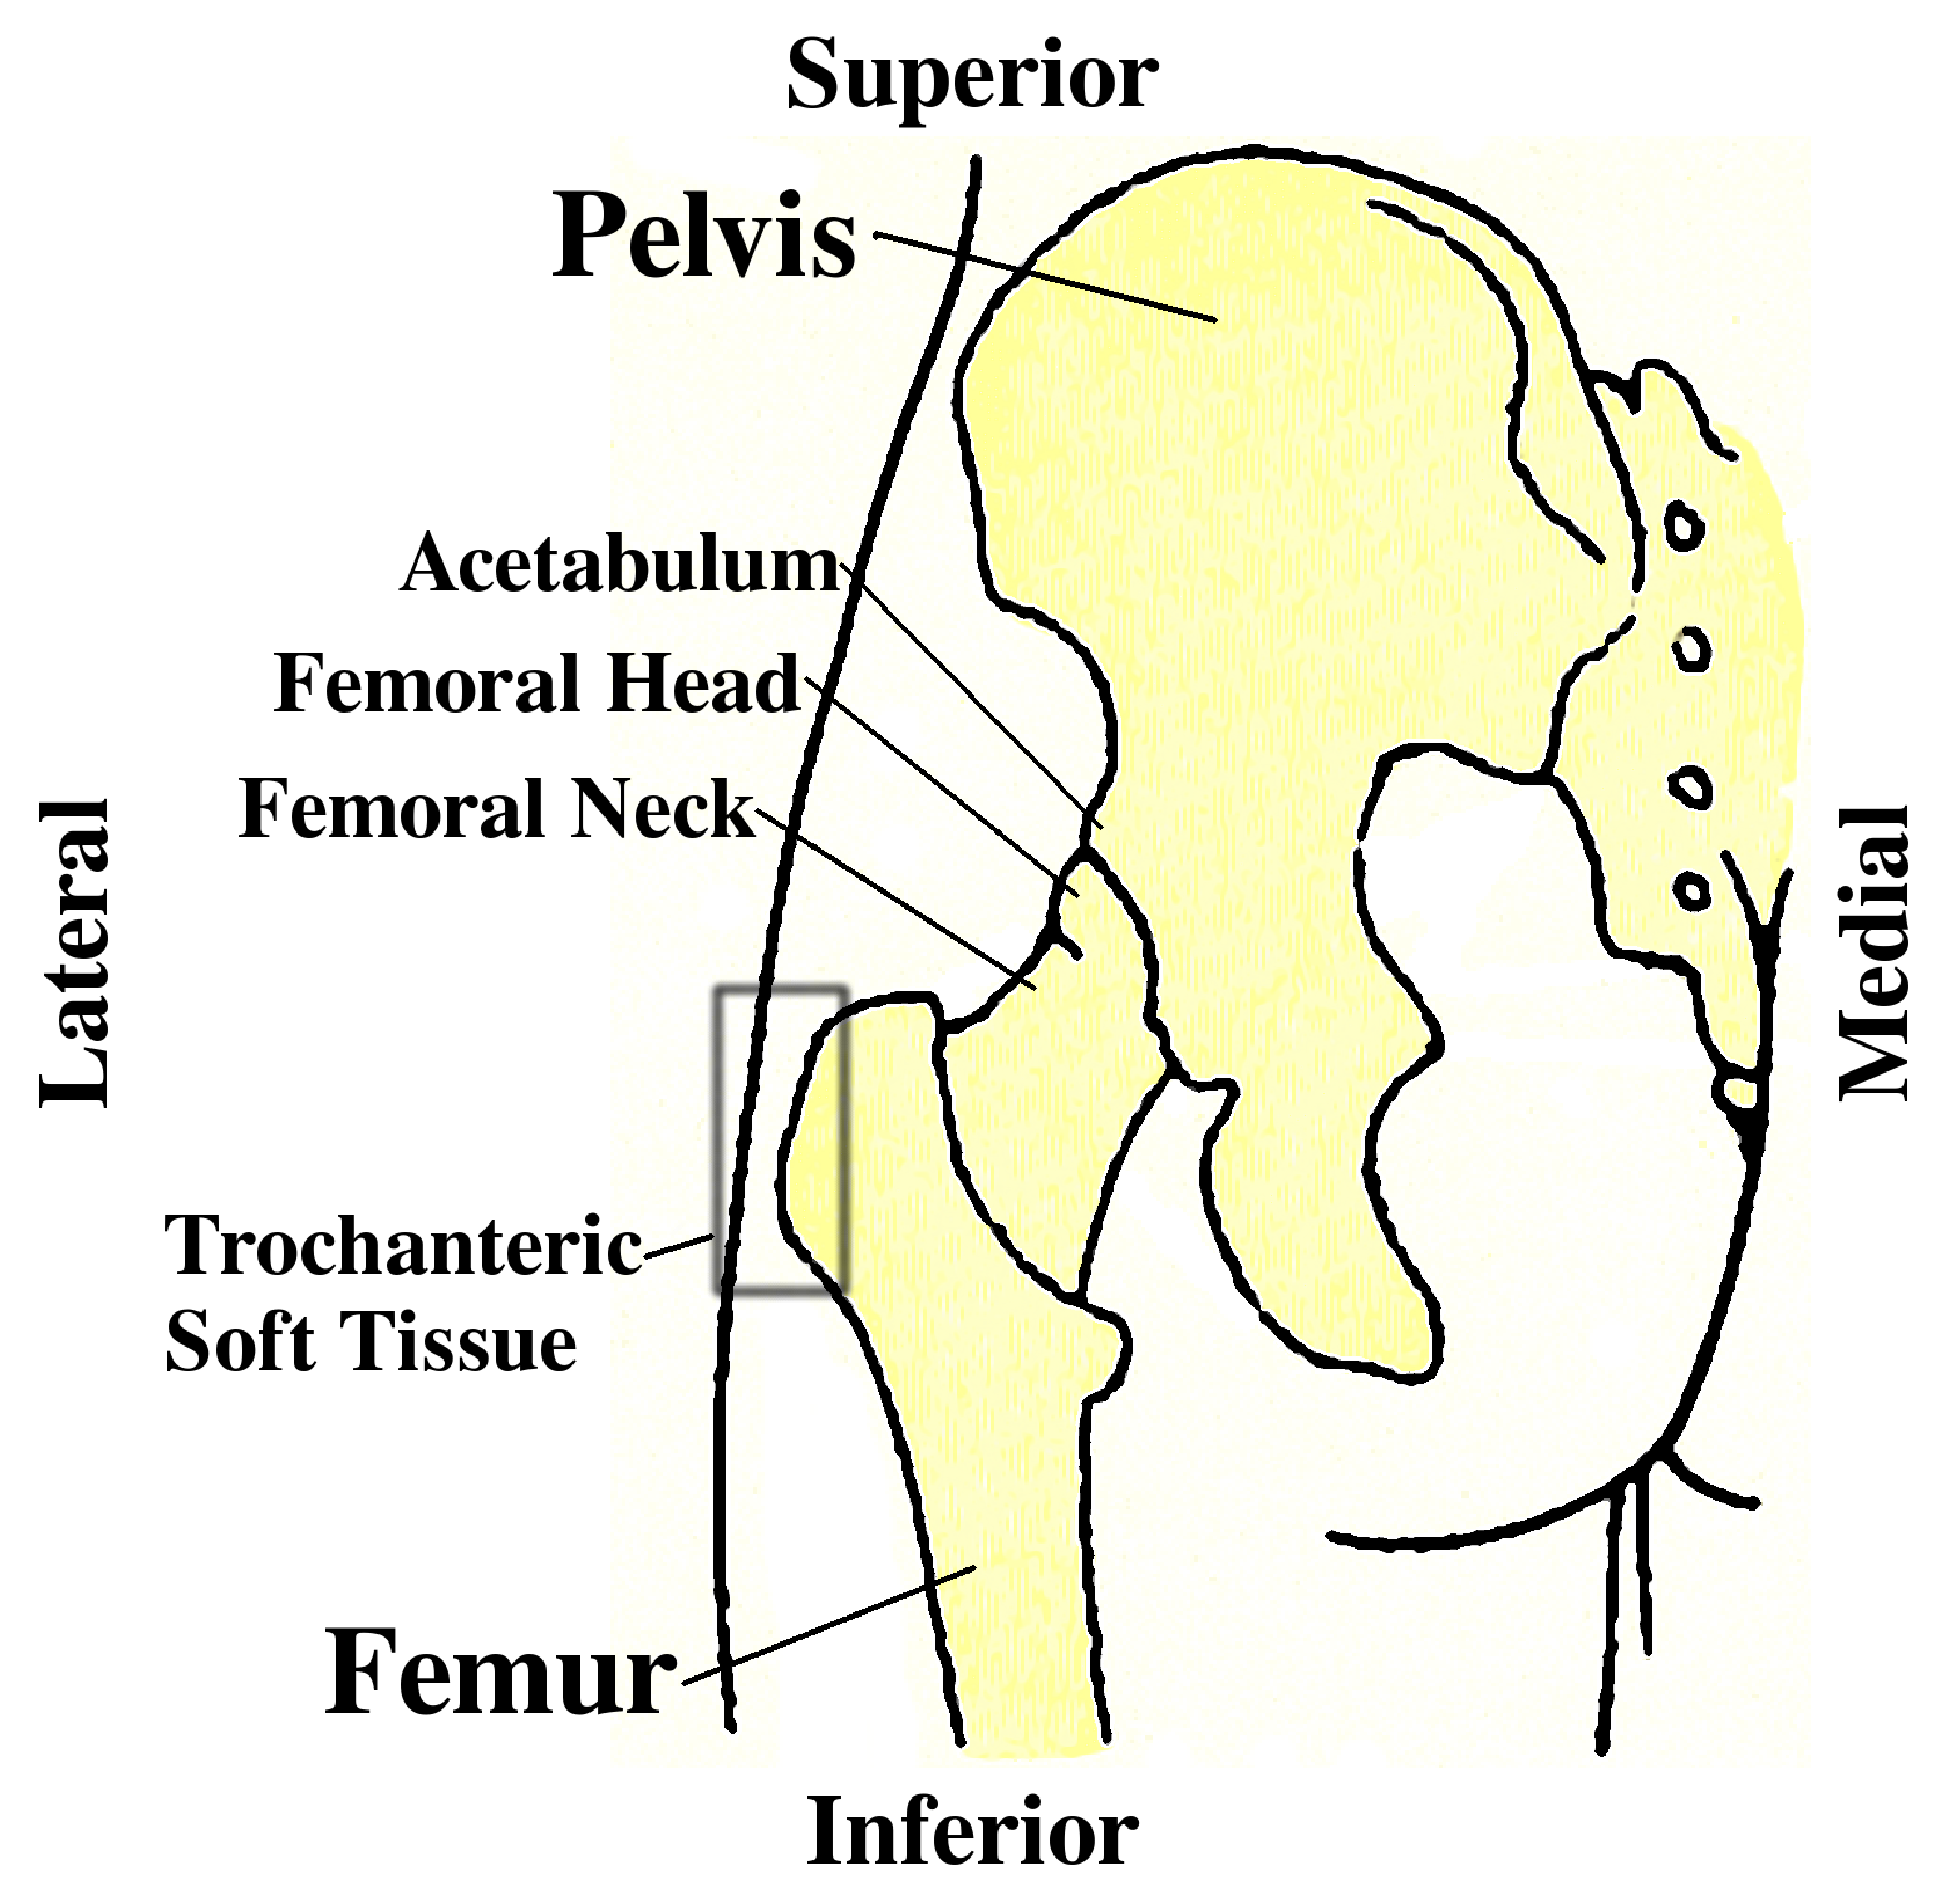
\includegraphics[width=\hsize]{./intro/Figures/Hip_Grays}
\caption[The hip joint]{\textbf{The hip joint is the junction of the trunk with the lower limb. This posterior view shows the pelvis on the medial side with the proximal femur on the lateral side of the joint.} Graphic adapted from~\citet{gray_anatomy_1918} (copyright expired).}
\label{fig:Hip}
\end{figure}

\subsection{Femoral anatomy}
\label{sec:intro_hipAnat_femur}
The femur is a large bone that is crucial for locomotion.
It has many muscle attachments and bony landmarks associated with those attachments.
The largest bony landmarks on the proximal end of the femur are the \textit{greater} and \textit{lesser trochanters} (Figure~\ref{fig:Femur}).
The region between these two landmarks is called the \textit{intertrochanteric region} and is relevant clinically as the site of approximately half of hip fractures~\citep{michelson_epidemiology_1995, lyritis_epidemiology_1996, sirois_burden_2009, lefaivre_changes_2011, poole_cortical_2012}.
The intertrochanteric region has a different morphology on the anterior and posterior aspects.
On the anterior side of the intertrochanteric region is the intertrochanteric \textit{line}, which runs from the supero-lateral greater trochanter to the lesser trochanter. On the posterior side is the intertrochanteric \textit{crest}, which has a similar path to the intertrochanteric line, running from the superio-lateral grater trochanter to the lesser trochanter.
The intertrochanteric crest is more prominent than the intertrochanteric line.

\begin{figure}
\centering
\includegraphics[height=.6\textheight]{./intro/Figures/Femur}
\caption[The femur]{\textbf{The femur, anterior (left) and posterior (right). The trochanters, linea aspera and epicondyles are the insertions of the muscles of the hip and knee joints.} Graphic \textcopyright Seth Gilchrist, 2013.}
\label{fig:Femur}
\end{figure}

Along the posterior aspect of the femoral shaft is the \textit{linea aspera}, which is the insertion for a number of muscles of both the knee and the hip joints.
There are a number of landmarks on the distal end of the femur, but the important ones for the current discussion are the \textit{condyles} and \textit{epicondyles}, which are used to define the coordinate system of the femur.
The condyles of the femur are the weight bearing portions of the distal femur.
The posterior and inferior condyles are approximately aligned with the coronal and transverse planes of the body, respectively in the anatomical position (Figure~\ref{fig:Planes_body}).
The epicondyles of the femur are associated with the colateral ligaments of the knee and are approximately aligned with the coronal plane of the body.

The coordinate system of the femur consists of two anatomical planes, with the third plane defined as orthogonal to the others (Figure~\ref{fig:Planes})~\citep{gray_anatomy_1918}.
The primary plane of reference is the \textit{femoral plane}, which is determined by the three most posterior points on the bone, typically the posterior condyles and trochanter, and is roughly parallel to the coronal plane of the body.
This plane can be thought of as the surface of a table when the bone is placed, posterior down, on the table.
Intraoperatively it is sometimes defined using the epicondyles rather than the posterior condyles, but the correlation between the two definitions is high and the difference small, with an average value of~2$^\circ$~\citep{dorr_comparison_2009}.

\begin{figure}
\begin{subfigure}{0.60\linewidth}
	\centering
	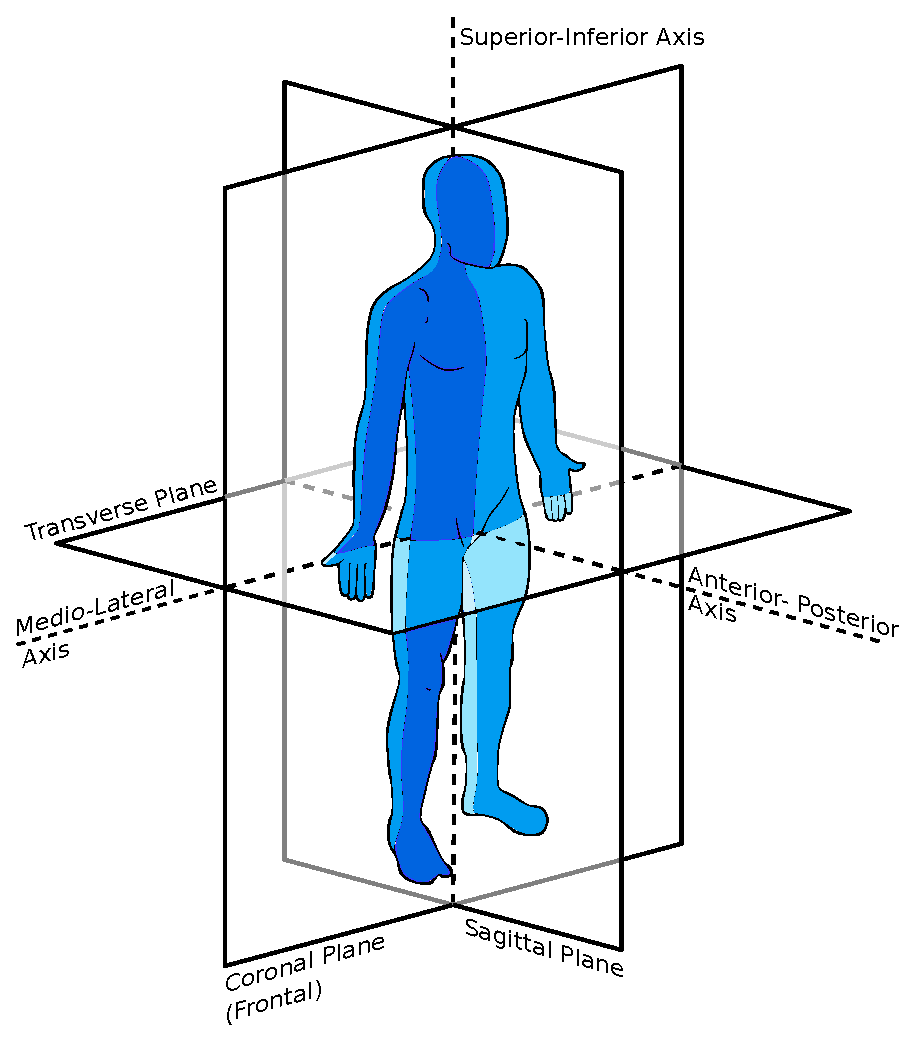
\includegraphics[width=\linewidth]{./intro/Figures/Anatomical-Planes-en}
	\caption{\textbf{Body} Graphic \citet{edoarado_anatomical_2011} (Creative Commons 3.0).}
	\label{fig:Planes_body}
\end{subfigure}
\begin{subfigure}{0.36725\linewidth}
	\centering
	
\includegraphics[width=\linewidth]{./intro/Figures/FemoralPlanes}
	\caption{\textbf{Femur} Graphic \textcopyright Seth Gilchrist, 2013.}
	\label{fig:Planes_femur}
\end{subfigure}
\caption[Anatomical and femoral geometrical references]{\textbf{Anatomical planes and directions for the body and femur. In (b), the femoral and condylar planes are labelled, and the mechanical plane is shown with transparency.} }
\label{fig:Planes}
\end{figure}

The second plane is the \textit{condylar plane}, and is defined as perpendicular to the femoral plane, and in contact with the inferior condyles.
It is roughly parallel to the transverse plane of the body.
The \textit{mechanical plane} is defined as perpendicular to the other two planes, passing through the centre of the femoral head, and is approximately parallel to the sagittal plane of the body.
This plane contains the mechanical axis of the femur, running from the centre of the femoral head to the point between the femoral condyles.

The femur has natural curves and twists that occur along its length.
The most obvious curve is the anterior bow of the femur~\cite{gray_anatomy_1918}, which is a bending of the shaft along its length, and occurs predominantly in the third plane.
A more subtle feature is the orientation of the femoral neck to the femoral plane, called \textit{femoral twist} or \textit{femoral version} (Figure~\ref{fig:Version}).
When the neck extends anteriorly to the femoral plane the bone is said to be anteverted, and if it extends posteriorly to the femoral plane it is said to be retroverted.
The femoral version can be measured in a number of different ways using different aspects of the neck to define its orientation.
Using the transverse mid-point of the lateral femoral neck and the centre of the femoral head is called the Kingsley-Olmsted method~\citep{kingsley_study_1948}, considered the clinical standard for version definition.
Other methods of measurement particular to modern imaging systems have also been devised, one example being the use of the anterior surface of the femoral neck as observed using ultrasound~\citep{aamodt_femoral_1995}.
Using the Kingsley-Olmsted method, the normal population has an anteversion angle of (mean(SD)) 9.73$^\circ$(9.82$^\circ$)~\citep{toogood_proximal_2009}.

\thisfloatsetup{floatwidth=0.5\textwidth,capbesidewidth=sidefil,capposition=beside,capbesideposition={top,right}}
\begin{figure}
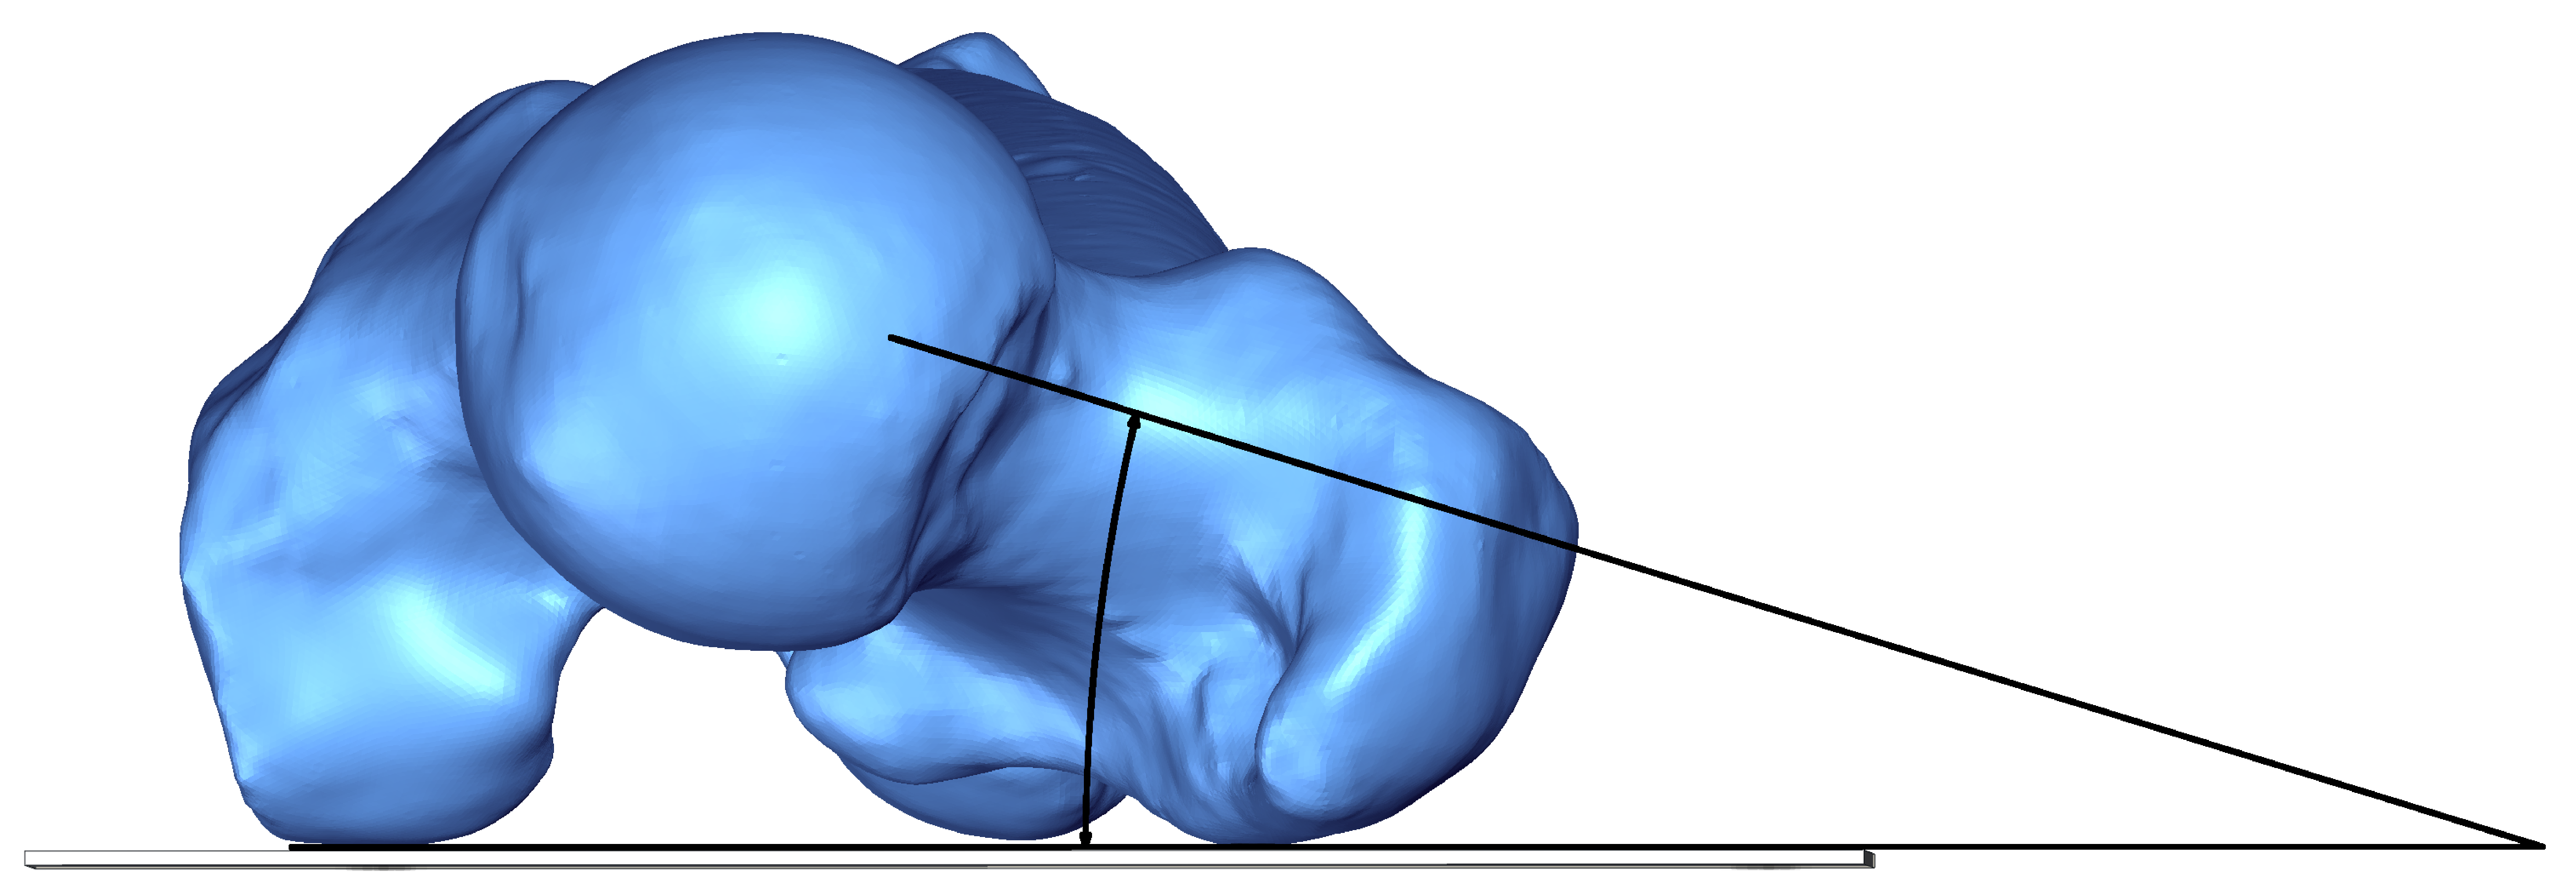
\includegraphics[width=\hsize]{./intro/Figures/Version}			
\caption[Femoral version]{\textbf{Femoral version is the acute angle between the neck and the femoral plane. It is measured by observing the angle from the superior aspect. This images shows the neck axis as defined using the Kingsley-Olmsted method~\cite{kingsley_study_1948}, where the midpoint of the lateral femoral neck is identified from the supero-lateral aspect and is connected to the centre of the femoral head. This specimen is anteverted by an angle of 15.2$^\circ$.} Image \textcopyright Seth Gilchrist, 2013.} 
\label{fig:Version}
\end{figure}

\subsection{Bone anatomy}
\label{sec:intro_boneAnat}
The bones of the body are important organs, with roles in support and movement as well as physiological homoeostasis.
They are composite structures with material types and properties that very spatially and in time.

At a material level, bone is made up of a collagen mesh that is mineralized by hydroxyapatite, and organized in a laminar fashion, making it strong and stiff.
At a structural level bone is classified into two types: cortical and cancellous (Figure~\ref{fig:bone_cancellous}).
Cortical bone (\acs{aka} compact bone) is primarily found in the shaft (or diaphysis) of long bones, and also makes up the exterior shell of irregular bones.
Cancellous bone (\acs{aka} spongy, or trabecular bone) is a low density network, consisting of columns and plates of bone that form a cellular solid.
It is found in the ends (or epiphyses) of long bones, and in the interior of most irregular bones.

\begin{figure}
\begin{subfigure}{0.49\linewidth}
	\centering
	\includegraphics[width=\linewidth]{./intro/Figures/Ascenzi_proximal}
\end{subfigure}
\begin{subfigure}{.49\linewidth}
	\centering
	\includegraphics[width=\linewidth]{./intro/Figures/Ascenzi_trabec}
\end{subfigure}
\caption[Cortical and cancellous bone images in the proximal femur]{\textbf{Left: A section of the proximal femur. Cortical bone serves as the exterior envelope of the organ, with cancellous bone in the interior. Right: Close up view of the cancellous bone showing plate-like (A) and rod-like (B) trabeculae.} Images adapted from~\citet{ascenzi_variation_2011} (with permission).}
\label{fig:bone_cancellous}
\end{figure}

There are two types of cortical bone, with names that refer to the organization of the collagen network: woven and lamellar.
\textit{Woven} bone is characterized by an unorganized, tangle of collagen Type-I fibres, and is mechanically weak.
In adults, woven bone is transient, created after injury where quick reinforcement is needed, and replaced by lamellar bone as healing progresses.

\textit{Lamellar} bone is characterized by long, laminarly organized, mineralized, collagen Type-I fibres.
Two subtypes of lamellar bone are commonly found in the appendicular skeleton: osteonal and interstitial.
Osteonal lamellar bone is contained within osteons (also called Haversian systems) which are concentric rings of lamellar bone that surround a central nutrient-transport canal (Figure \ref{fig:Compact_bone}).
The collagen fibres in the bone of the Haversian systems are oriented in roughly the same direction, but can be as much as 90$^\circ$ off from adjacent layers (both running 45$^\circ$ from the osteon axis).
Interstitial lamellar bone consists of fragments of lamellar bone that fill the gaps between Haversian systems.

\thisfloatsetup{floatwidth=0.5\textwidth,capbesidewidth=sidefil,capposition=beside,capbesideposition={top,left}}
\begin{figure}
\includegraphics[width=\hsize]{./intro/Figures/Compact_bone}			
\caption[Cortical bone cross-section]{\textbf{A cross-section of cortical bone at high resolution. The concentric rings are lamellar bone (each about 5~\ac{micro-m} thick), organized into Haversian systems. The spaces between the Haversian systems contain interstitial lamellar bone.}. Image courtesy of~\citet{konrad_compact_2009} (public domain).}
\label{fig:Compact_bone}
\end{figure}

Cortical bone is quantified using either density (\acs{g}/\acs{cm}$^3$), or \acf{bv/tv} in conjunction with beam section properties such as the second area moment of inertia.

Cancellous bone is also made up of lamellar bone; however, the mesioscale (\acs{ie}, between micro- and macroscale) organization of cancellous bone gives it significantly different structural properties.
It has an open cell structure that is made up of discrete rod- and plate-like trabecular elements (Figure \ref{fig:bone_cancellous}).
This structure means that cancellous bone is much softer and better at absorbing energy than cortical bone.
The organization of the cellular matrix is critical to the behaviour of the material, and quantification of this structure is done in a number of ways (Table \ref{tab:cancellous}).

% % Define a new command to allow for multiple rows in one cell
% command def from http://tex.stackexchange.com/questions/83757/aligning-text-in-a-table
\newcommand{\lbCell}[2][c]
{ 
\begin{tabular}[#1]{ c }
	#2
\end{tabular}
}

\begin{table}
\footnotesize
\centering
\caption[Trabecular quantification]{Trabecular quantification measures. Many more that have been proposed, but these are the most common.}
\label{tab:cancellous}
\begin{tabular}{l c c m{7cm}}
\toprule
Quantity & Measure  & Units & Description \\
\midrule
Density 	& \lbCell{Bone Volume Ratio \\ (\acs{bv/tv} or V$_V$)} 		& $\frac{mm^3}{mm^3}$  & Ratio of bone volume to total volume in a given \ac{roi}.\\ \hline
Surface Area& \lbCell{Surface Volume Ratio \\  (\acs{bs/tv} or S$_V$)}	& $\frac{mm^2}{mm^3}$ & Ratio of bone surface area to total volume in a given \ac{roi}.\\  \hline
\multirow{2}{2cm}{Trabecular Dimensions}
		& \lbCell{Trabecular Thickness \\ (\acs{tbth})}	& $mm$ & Average trabecular thickness calculated in a random, \ac{2d} slice. \\[1EX] 
			& \lbCell{Trabecular Spacing \\ (\acs{tbsp})} 	& $mm$ & A measure of spacing between trabeculae, derived using a parallel-plate, theoretical model of trabecular morphology. \\ \hline
Anisotropy & \lbCell{Mean Intercept Length \\ (\acs{mil})}	& $mm$ & A measure of the material fabric orientation, derived from \ac{2d} sections, which indicates the number of intersections along a projection from a randomly selected point. Provides a tensor, with the first and third Eigenvectors indicating the maximum and minimum material directions.\\ \hline
\multirow{3}{*}{Topology}
		& \lbCell{Trabecular Number \\ (\acs{tbn})} 		& $\frac{1}{mm}$ & A measure indicating the number of trabeculae in a given volume. Derived using a parallel-plate, theoretical model of trabecular morphology.\\
		& \lbCell{Connective Density \\ (\acs{connd})}	& $\frac{1}{mm}$ & A measure of the number of trabecular intersections. \\
		& \lbCell{Structure Model Index \\ (\acs{smi})}	& unitless  & A measure of morphology as more rod or plate like. An ideal rod structure has an \acs{smi} of 0 and an ideal plate structure has an \acs{smi} of 3.\\
\bottomrule
\end{tabular}
\end{table}

An especially important cancellous bone measurement for the current discussion is the \ac{mil}, which quantifies the orientation of the trabecular network and is important when evaluating material anisotropy.
The \ac{mil} is determined from \ac{2d} sections on which lines at various angles are drawn. The average distances between trabeculae on the lines are recorded at each angle (Figure~\ref{fig:Odgaard_MIL}).
This measurement yields a tensor which defines the fabric properties in any given cut of the bone.
The Eigenvectors and Eigenvalues of the tensor can then be used to determine the principal directions, in much the same way that principal stresses can be determined from the Eigenvectors and values of a stress tensor (Figure~\ref{fig:Eigenvectors}).

\thisfloatsetup{floatwidth=0.5\textwidth,capbesidewidth=sidefil,capposition=beside,capbesideposition={top,right}}
\begin{figure}
\includegraphics[width=\hsize]{./intro/Figures/Odgaard_MIL}
\caption[Determination of \acs*{mil}]{\textbf{A bone cross-section showing the lines used to determine the \acs{mil}. The average distance between the trabeculea along the lines is recorded at various values of the angle $\omega$. An image slice in a perpendicular direction will give the \ac{mil} in the out-of-image dimension.} Graphic adapted from \citet{odgaard_three-dimensional_1997} (with permission).}
\label{fig:Odgaard_MIL}
\end{figure}

\thisfloatsetup{floatwidth=0.5\textwidth,capbesidewidth=sidefil,capposition=beside,capbesideposition={top,left}}
\begin{figure}
\includegraphics[width=\hsize]{./intro/Figures/Ascenzi_trabec_eigenvectors}
\caption[\acs*{mil} of a \acs*{2d} section]{\textbf{Eigenvectors are a mathematical tool for identifying important directions in systems described by tensors. In the case of fabric tensors, like those used for \ac{mil}, the first Eigenvector will point in the direction where most of the bone is oriented. The second and third Eigenvectors will be perpendicular to the first (and each other) and will point in the directions of the other two main material directions. In this \acs{2d} depiction, the first Eigenvector points along the strongest trabeculae and the second points in the perpendicular direction, along transverse supports.} Image adapted from~\citet{ascenzi_variation_2011} (with permission).}
\label{fig:Eigenvectors}
\end{figure}

\section{Fractures of the proximal femur}
\label{sec:intro_fractures}
Fractures of the proximal femur are an important social and clinical problem in Canada and around the world.
They constitute a large proportion of all orthopaedic injuries, with some studies reporting more than 20\% of orthopaedic beds being occupied by hip fracture patients at any given time~\citep{torgerson_letter:_2000}.
While research has shown a trend of decreasing fracture rates in recent years~\citep{lefaivre_changes_2011}, the total incidents of fracture is increasing as the population ages~\citep{wiktorowicz_economic_2001}, and the hospital admissions are becoming more complex, with increasing number of comorbidities~\citep{sirois_burden_2009}.

Fractures are thought to be caused in two ways.
The first, and likely the most common, is as a result of a fall to the side; the second, and less common, is a spontaneous fracture due to extreme bone fragility.
While both types of fractures are important, the focus of the current work is on fractures due to falls as they are thought to constitute upwards of 95\% of hip fracture cases~\citep{parkkari_majority_1999}.

The financial impact of the fractures on the health care system is difficult to overstate.
The 1-year cost of an individual fracture in Canada has been put in the range of CDN\$29,065 -- \$60,013 (\citep{wiktorowicz_economic_2001}, corrected to 2013 dollars by the Bank of Canada~\citep{bank_of_canada_inflation_2013}).
Lifetime costs of a single hip fracture in the US are as high as US\$107,193 (\citep{braithwaite_estimating_2003}, corrected to 2013 dollars by the US Bureau of Labor Statistics~\citep{bureau_of_labor_statistics_cpi_2013}).
All together, these fractures cost the Canadian system CDN\$659M/year (\citep{tarride_burden_2012}, corrected to 2013 dollars by the Bank of Canada~\citep{bank_of_canada_inflation_2013}), and this value could more than double by 2040~\citep{wiktorowicz_economic_2001}.

Considerable work has been performed by the research community to understand and prevent hip fractures.
This section will describe the clinical procedures and burdens of hip fracture, and the research that has been conducted to reduce that burden.

\subsection{Clinical considerations}
\label{sec:fractures_clinic}
Hip fracture is a significant clinical problem, and an understanding of the needs and requirements of the clinical situation is key to developing a meaningful treatment or mitigation strategy.
Clinical interventions begin with screening and, if indicated, continue with prophylactic prescription of either drugs or biomechanical devices, such as hip protectors.
If screening and prevention fail, and a hip fracture results, the most common clinical treatment is surgical repair using plates, screws or full joint components.
There are a variety of surgical options depending on the details of the fracture.

\subsubsection{Early risk assessment}
\label{sec:fractures_clinic_risk}
The primary risk factors for hip fracture are age, falling, and bone density~\citep{cummings_risk_1995}.
Risk assessment and clinical treatment targets are therefore geared towards assessing and addressing these factors.
There are a number of preventative interventions that have shown some success, such as pharmacological~\citep{hodsman_bisphosphonates_2002}, lifestyle~\citep{moayyeri_association_2008} and to some degree hip protectors~\citep{haines_hip_2006}.
The first step to implementing one of these possible treatments is identification of individuals at risk of hip fracture through screening.
The gold standard screening technique is \acf{dxa} to quantify \acf{bmd}, which is then used to evaluate osteoporosis state.

Osteoporosis is a clinical diagnosis of low \ac{bmd}.
It is not a disease in itself, but a condition caused by a number of possible aliments, including vitamin-D deficiency, hormone deficiency, or physiological ageing~\citep[Ch.12]{avioli_metabolic_1998}.
Two metrics exist for rating an individual's bone density.
The \textit{T-score} shows where an individual's \ac{bmd} falls in comparison to a sex and race match young adult population (Equation \ref{equ:tscore}), and the \textit{Z-score} shows where an individual's bone density falls in relation to a sex, race and age-matched population (Equation \ref{equ:zscore})~\citep{orwoll_osteoporosis_2011}.
The definition of osteoporosis state, as given by the \ac{who}, uses the T-score (Table \ref{tab:op}).

\begin{eqnarray}
	\label{equ:tscore}
	T &=& \frac{BMD_{patent} - \overline{BMD}_{lifetime\; peak}}{\acs*{sd}_{lifetime\; peak}} \\ [1em]
	\label{equ:zscore}
	Z &=& \frac{BMD_{patent} - \overline{BMD}_{age-matched}}{\acs*{sd}_{age-matched}}
\end{eqnarray}

\begin{table}
	\caption[\acs*{who} osteoporosis definitions]{\acs*{who} definition of osteoporosis state~\citep{who_study_group_assessment_1994}.}		
	\label{tab:op}
	\begin{tabularx}{0.9\textwidth}{l X}
		\toprule
		\textbf{Classification} & \textbf{Description} \\ \midrule
		Normal                  &  \ac{bmd} greater than 1~\acs{sd} below the young adult average ($T > -1$). \\
		Osteopenia              &  \ac{bmd} between 1 and 2.5~\acs{sd} below the young adult average ($-1 \geq T > -2.5 $).\\
		Osteoporosis            &  \ac{bmd} less than 2.5~\acs{sd} below the young adult average ($T \leq -2.5$).\\ \bottomrule
	\end{tabularx} 
\end{table}

\ac{dxa} is an x-ray imaging technique that provides a measure of mineralized bone content between the x-ray source and collector.
Since a \ac{2d} image is created, the output of the technique is commonly called the \ac{abmd}, in which the \ac{bmc} is normalized by the projected area, and is quantified in units of~$\acs{g}/\ac{cm}^2$.
To measure \ac{bmc}, the \ac{dxa} method breaks the human body into two components: soft tissue and bone mineral.
The soft tissues of the body all have approximately the same x-ray attenuation, which is significantly lower than that of bone mineral.
With only two components, the amount of each can be found by simultaneously solving the Beer-Lambert relation at two energy levels (Equations~\ref{equ:dxa1} and~\ref{equ:dxa2})~\citep{jacobson_x-ray_1964, gustafsson_x_1974}.

\begingroup
\setlength{\abovedisplayskip}{-2ex}
\begin{eqnarray}
\label{equ:dxa1}
	I_1 = I_{0,1} \cdot e^{-(\mu_{1,t} \cdot x_t + \mu_{1,b} \cdot x_b)} \\ [1ex]
\label{equ:dxa2}
	I_2 = I_{0,2} \cdot e^{-(\mu_{2,t} \cdot x_t + \mu_{2,b} \cdot x_b)} 
\end{eqnarray}
\endgroup

\acused{n/eng} \acused{i/eng} \acused{mu/attn} \acused{x/dxa} \acused{t/dxa} \acused{b/dxa} % acronyms that are spelled out below

\ac{i/eng}$_{0,n}$ and \ac{i/eng}$_n$ are the incident and transmitted x-ray intensities at energy level $\ac{n/eng}$, respectively.
\ac{mu/attn}$_{n,t}$ and \ac{mu/attn}$_{n,b}$ are the linear attenuation coefficients at energy level \ac{n/eng} for the \acf{t/dxa} and \acf{b/dxa}, and \ac{x/dxa}$_t$ and \ac{x/dxa}$_b$ are the path lengths in the \acl{t/dxa} and \acl{b/dxa}.
The transmitted and incident energy levels, as well as the absorption coefficients, are known \textit{a priori}, and therefore the path lengths can be solved.
The product of the known density of bone mineral ([\ac{kg}/\ac{m}$^3$]) with the calculated path length ([\ac{m}]) is \ac{abmd} ([\ac{kg}/\ac{m}$^2$]).

Modern \ac{dxa} machines include internal calibrations of known path lengths to ensure accuracy~\citep{guillemot_pelvic_1997}; however, there are a number of issues that must be considered when calculating \ac{abmd} using \ac{dxa}~\citep{bolotin_patient-specific_2003}.
To begin with, data from \ac{dxa} machines cannot be readily compared across manufacturers~\citep{genant_universal_1994}.
Each manufacturer creates a custom database of population \acp{abmd}, making it possible to compare T- and Z-scores. However, direct comparison of \ac{abmd} values must be corrected based on a standard calibration performed on each machine~\citep{genant_universal_1994}.

Secondly, the changes in bone quality can happen in either the cancellous or cortical compartments.
Cancellous bone, by its very nature, has a lower projected density than cortical bone, and therefore makes up a smaller portion of the $x_b$ in Equations \ref{equ:dxa1} and \ref{equ:dxa2}.
In the early stages of bone loss, cancellous bone changes can be more pronounced than cortical bone changes, but may not be detected by \ac{dxa} screening~\citep{guglielmi_osteoporosis:_1994}.

Third, spurious calcification of the bones and/or adjacent structures can interfere with \ac{dxa} measurements.
Osteophytes (calcification of bone in non-load-bearing regions) are common in the elderly~\citep{rand_impact_1997}, and have a significant effect on \ac{abmd} readings~\citep{rand_impact_1997}.
Adjacent structures can be ossified ligaments and cartilage or calcium deposits in the aorta, which runs adjacent to the spine~\citep{smith_aortic_1999}.
Calcification of these structures will increase the derived \ac{abmd} and lead to an inappropriate osteoporosis classification.

The final problem is caused by projection issues due to the size of the bone being scanned, versus the average size of the bone in the reference population.
In the projection of an object, the volume increases faster than its projected area as its characteristic length increases.
This can lead to bones that are significantly larger than the reference population having higher \ac{abmd}, which may be mistaken for higher \ac{bmc}~(see \S\ref{sec:support_abmd} for an example calculation).

In order to address some of these limitations, the \ac{who} developed the \ac{frax} which can be used either in conjunction with \ac{bmd} measurements, or as an independent analysis~\citep{kanis_fraxtm_2008}.
The \ac{frax} score is based on twelve risk factors and provides a 10~year probability of spine, humerus or wrist fracture, as well as a 10~year probability of hip fracture (Table~\ref{tab:frax}).

\begin{table}
\caption[Inputs to the \acs*{frax} model]{Inputs into the \acs*{frax} model. The inclusion of \ac{bmd} is optional~\citep{kanis_fraxtm_2008, van_den_bergh_assessment_2010}.}
\label{tab:frax}
\begin{tabularx}{0.75\textwidth}{>{\centering\arraybackslash}X >{\centering\arraybackslash}X}
\toprule
\textbf{Risk Factor} & \textbf{Data} \\ 
\midrule
 Age & Years \\ 
 Gender & Male or Female \\ 
 Weight & \ac{kg} \\ 
 Height & \ac{cm} \\ 
 Previous Fracture & Yes or No \\ 
 Parent Fractured Hip & Yes or No \\ 
 Current Smoking & Yes or No \\ 
 Glucocorticoids & Yes or No \\ 
 Rheumatoid Arthritis & Yes or No \\ 
 Secondary Osteoporosis & Yes or No \\ 
 Alcohol $\geq$3 units per day & Yes or No \\ 
 Femoral Neck \ac{bmd} & T-score or Z-score \\ 
\bottomrule 
\end{tabularx} 
\end{table}

The \ac{frax} tool must be calibrated for each population for which it is used, as the weighting of each risk factor cannot be generalized.
Once it has been calibrated, \ac{frax} can help identify those at risk of fracture.
The efficacy of the tool is dependent on the probability cutoffs used.
For example, if a 10~year fracture probability of 20\% is used as a cutoff, nearly 30\% of those who will suffer a fracture can be identified~\cite{leslie_fracture_2011}.
While identification of 30\% of individuals is high, it is only moderately higher than the 28\% that can be identified by osteoporosis score alone~\citep{stone_bmd_2003}, and has been shown to be no better than using only \ac{bmd} + age and neglecting the other ten risk factors~\citep{van_den_bergh_assessment_2010}.
A major strength of the \ac{frax} tool is that an initial assessment can be conducted without the need for a \ac{dxa} scan, and if the individual is found to be in an intermediate risk group, a \ac{dxa} scan can be performed and the person's risk level re-evaluated~\citep{kanis_frax_2009}.

Keeping these limitations in mind, \ac{frax} and \ac{dxa} provide simple, fast and useful clinical tools.
\ac{dxa} provides a single number (in the case of \ac{abmd}) or designation (in the case of osteoporosis state) that indicates a clinical course of action.
\ac{frax} can be used as a pre-screening tool for \ac{dxa} scanning and can refine the individual risk if \ac{dxa} scanning is indicated.
The \ac{who} recommends screening women over the age of 65, which is a significant screening burden, and while uptake is high, it is not 100\%~\citep[p.~101]{who_study_group_assessment_1994}.
The \ac{who} also recognizes the fact that many individuals who are screened using these tools and found to be free from osteoporosis will still go on to fracture~\citep[p.~99]{who_study_group_assessment_1994}.
		
\subsubsection{When screening fails}
\label{sec:fractures_clinic_fail}
Even for those who undergo screening, falls cannot always be avoided, and hip fracture cannot always be prevented.
Depending on the fracture type, location, and any comorbidities, there are a number of treatment options available to clinicians -- most of them surgical.

Patients that present with hip fracture due to fagility are typically older and female~\citep{cummings_epidemiology_2002}.
After initial assessment has indicated a possible hip fracture, anterior-posterior x-rays of the hip are used to classify of the fracture type, which guides treatment.

Fracture classification is hierarchical and helps to indicate the appropriate intervention.
The highest level is intracapsular vs.\ extracapsular fracture, which references the fracture location in terms of whether it is located inside or outside the joint capsule (Figure~\ref{fig:HipCapsule}).
Intracapsular fractures are fractures of the femoral neck and are further classified into basicervical, cervical or subcapital fractures (Figure \ref{fig:NeckFractues}).
Basicervical fractures occur in the femoral neck, at the junction with the trochanter; cervical fractures occur somewhere along the length of the neck; and subcapital fractures occur at the base of the femoral head.

\begin{figure}
\centering
\includegraphics[width=0.7\linewidth]{./intro/Figures/HipCapsule}
\caption[The hip joint capsule]{\textbf{Posterior view of the hip showing the hip joint capsule. The capsule comprises the blue membrane, which has been distended in this view for visualization.} Graphic adapted from~\citet{gray_anatomy_1918} (copyright expired).}
\label{fig:HipCapsule}
\end{figure}

Extracapsular fractures are sub-classified into intertrochanteric, trochanteric, or subtrochanteric (Figure~\ref{fig:ExtracapFractues}).
Intertrochanteric (\acs{aka} pertrochanteric) fractures run between the greater and lesser trochanters, just lateral to the line of a basicervical fracture; trochanteric fractures involve only one of the trochanters; and subtrochanteric fractures involve the femoral diaphysis, distal to the lesser trochanter. 
The proportions of each fracture type are roughly 45\% intracapsular, 55\% extracapsular; however, that ratio seems to be changing, with a tendency to fewer intracapsular fractures~\citep{haleem_mortality_2008}.

\begin{figure}
	\centering
	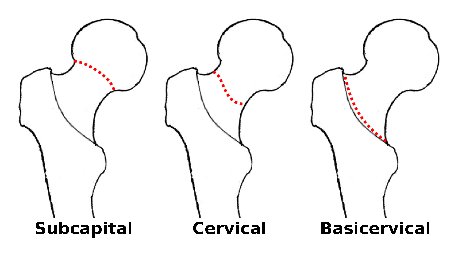
\includegraphics[width=0.7\linewidth]{./intro/Figures/NeckFractues}
	\caption[Intracapsular fractures]{\textbf{Intracapsular fractures of the proximal femur.} Graphic \copyright Seth Gilchrist, 2013.}
	\label{fig:NeckFractues}
\end{figure}

\begin{figure}
	\centering
	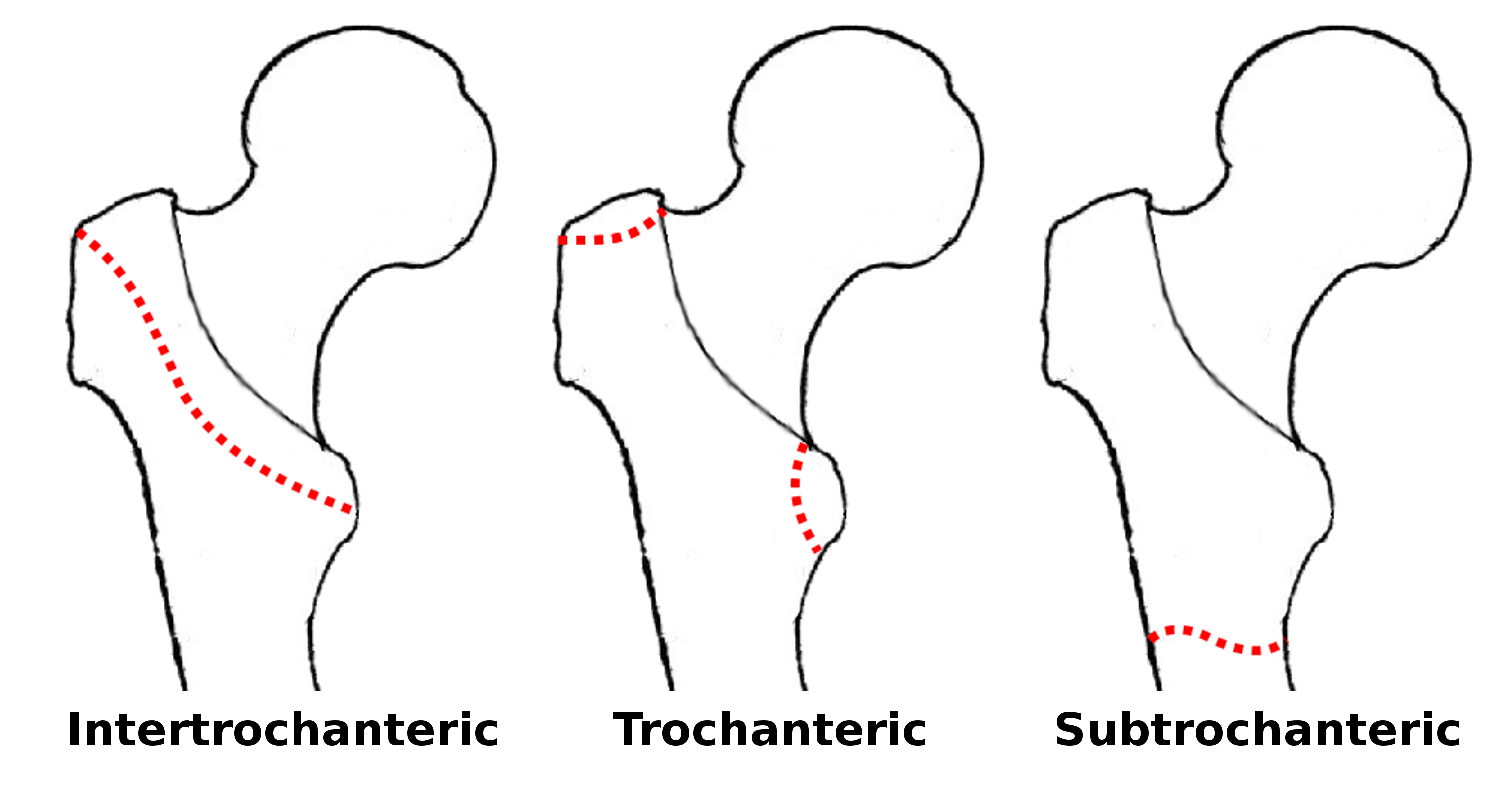
\includegraphics[width=0.7\linewidth]{./intro/Figures/ExtracapFractues}
	\caption[Extracapsular fractures]{\textbf{Extracapsular fractures of the proximal femur.} Graphic \copyright Seth Gilchrist, 2013.}
	\label{fig:ExtracapFractues}
\end{figure}

There are two surgical strategies for hip fracture treatment: repair and replacement.
Surgical repair of proximal femur fractures involves reduction and fixation, while surgigal replacement includes hemiarthroplasty, and \ac{tha}.
Reduction is the process of aligning fractured fragments, which are then secured in place using fixation, typically utilizing plates, rods screws and/or nails.
Reduction can be either \textit{open}, in which the fragments are dissected, and oriented manually, or \textit{closed}, where external pressure and traction are used to align fragments.
\ac{tha} involves resection of the femoral head and neck, reaming of the acetabular cup, and replacement of these components with a stem and ball on the femoral side and an articulating cup on the pelvis side.
In hemiarthoplasty, this procedure is done only on the femoral side and the acetabular anatomy is left in place.

The indications for the type of surgical solution can be quite complex~\citep{simon_emergency_2011, browner_skeletal_2002}.
They rely on the location of the fracture~\citep{bray_femoral_1997, delamora_introduction_2002}, the angle of the fracture line~\citep{bray_femoral_1997}, the age of the patient~\citep{shah_algorithms_2002,bhandari_internal_2003}, time since fracture~\citep{bray_femoral_1997, delamora_introduction_2002}, and any comorbidities~\citep{shah_algorithms_2002, bhandari_internal_2003}.
Depending on the severity and type of comorbidities, surgery may not be an option, in which case non-operative treatment may be required.
Non-operative treatment of hip fracture has shown poor outcomes and is not common~\citep{heim_nonoperative_2002}.
It requires an extended period of non-weight bearing ($\sim$6~weeks), which can exacerbate existing bone quality issues, and has been seen to have poorer long-term outcomes compared to repair or replacement strategies~\citep{heim_nonoperative_2002}.

Hip surgery has a high success rate~\citep{heim_nonoperative_2002, bhandari_internal_2003, browner_skeletal_2002}, and is the preferred treatment option for hip fracture.
That said, hip fracture is a very serious injury and can result in a decrease in quality of life, extended morbidity, and even mortality.
\citet{wiktorowicz_economic_2001} found 38.4\% of community dwelling individuals who suffered hip fractures were discharged into either assisted living (27.1\%), or died (11.3\%).
This is corroborated by another study that found 26\% of community dwelling individuals were discharged to assisted living after hip fracture~\citep{cooper_crippling_1997}.
Additionally, hip fracture patients spend more time in assisted living than age-matched controls -- an average of 237 more days than a typical 80 year old~\citep{braithwaite_estimating_2003}.

Mortality following hip fracture is also high.
While death generally isn't directly attributable to the fracture, hip fracture patients fare much worse than their age-matched controls due to a range of systemic deleterious health effects~\citep{cooper_crippling_1997}. 
In the three months following hip fracture, patients have a mortality \ac{or} of 2.8 over age-matched controls~\citep{richmond_mortality_2003}.
This gradually decreases back to an \ac{or} of 1.4 at two years, but mortality rates remain higher than age-matched controls for at least five years post fracture~\citep{cooper_crippling_1997}.
In actual percentages of patients, one year post fracture, up to 21.6\% of patients have died~\citep{wiktorowicz_economic_2001}.

This section has discussed the clinical screening, treatment and discharge paths of hip fracture patients.
The treatment and discharge sections show just how important screening is.
Research conducted to improve screening efficacy is of clear benefit to patients and society.
Only with accurate screening abilities will we be able to concentrate our prevention efforts -- be they pharmacological, lifestyle or surgical strengthening -- on the most vulnerable people. 

\section{Mechanical behaviour of bone}
\label{sec:intro_boneBehaviour}
Before addressing hip fracture test methods and models, the mechanical behaviour of the materials that comprise the proximal femur need to be understood.
In Section~\ref{sec:intro_hipAnat} I discussed the anatomy of the femur and the bone were discussed.
This section builds on that knowledge by outlining the mechanical behaviours of these materials based on anatomical and morphological differences.
Following this discussion of the mechanical behaviours, the different methods for modelling hip fracture will be discussed, in which the material level behaviours will be important.

The bones of the body are complex organs that are made up of multiple materials serving a variety of functions.
The principal load bearing material is named after the organ itself and is called \textit{bone}.
Bone material is inhomogeneous, anisotropic and viscoelastic.
This means that its mechanical properties vary with location, loading direction, and loading speed.
These facts make determination of bone mechanical properties challenging.

Mechanical characterization of bone is done using traditional materials testing methods in which specimens are formed into regular geometries and stretched, compressed or sheared.
Cortical bone is typically milled into dog-bone specimens for tensile testing, and either cuboidal or cylindrical specimens for compression testing~\citep{currey_effects_1975, reilly_elastic_1975, evans_response_1992}.
In cortical bone, the ``orientation" of the specimen is determined by how the loading axis is aligned with the axis of the predominate Haversian system.
Bone is a linearly elastic material, and as such can be characterized in the elastic loading regime using the modulus of elasticity.
The modulus of elasticity of cortical bone varies depending on the orientation of loading (Table \ref{tab:bone_behave}).
It is highest in the longitudinal direction (aligned with the collagen fibrils), and lowest in the transverse direction.

\begin{table}[t]
\caption[Elastic properties of bone]{Approximate cortical and cancellous bone material properties~\citep{reilly_elastic_1975, lotz_mechanical_1991, rincon-kohli_multi-axial_2009}. Longitudinal is along the principal material direction, which is defined by the Haversian system in cortical bone and the first Eigenvector of the \ac{mil} tensor in cancellous bone. Transverse is perpendicular to the Haversian system in cortical bone, and along the third Eigenvector of the \ac{mil} tensor in cancellous bone.}
\label{tab:bone_behave}
\begin{tabularx}{0.8\textwidth}{l l >{\centering\arraybackslash}X >{\centering\arraybackslash}X }
\toprule
				&					& 	\multicolumn{2}{c}{Bone Type}	\\
Modulus (GPa)	& Direction			& Cortical 			& Cancellous	\\	\midrule
Tensile			& Longitudinal		& 17.9				& 2.0			\\
 				& Transverse		& 10.1 				& 0.2			\\[1EX]
Compressive		& Longitudinal		& 18.2				& 9.5			\\
				& Transverse		& 11.7 				& 5.5			\\[1EX]
Shear 			& Transverse		& 3.5				& 0.017			\\
\bottomrule			
\end{tabularx}
\end{table}

Cancellous bone is typically milled into cuboidal or cylindrical specimens for testing~\citep{helgason_mathematical_2008}, with the orientation often given in a site-specific manner~\citep{carter_compressive_1977, fyhrie_failure_1994, nazarian_densitometric_2007}.
For example, the testing direction for cancellous bone of the femoral neck will be given as parallel or perpendicular to the femoral neck axis.
It is becoming more common to also report the orientation with reference to fabric properties, such as \ac{mil}~\citep{rincon-kohli_multi-axial_2009}.
Using the anatomical reference, longitudinal loading is along the direction of the site-specific principal length (\ac{eg}, along the femoral neck); however, using the fabric properties, longitudinal loading is along the first Eigenvector of the fabric tensor~(Figure~\ref{fig:Eigenvectors}.
Transverse loading is perpendicular to the longitudinal direction.
When used with site-specific reference the term \textit{transverse} does not give any information regarding the direction in the plane perpendicular to the principal length in which the loading is taking place.
For example, transverse loading of a femoral neck specimen would be radial loading of the femoral neck bone; however, the direction of the radial (\ac{eg}, anterior-posterior) would not be given.
When fabric properties are used, researchers will normally give the Eigenvector along which they are loading, rather than using term transverse. For example, a specimen subjected to transverse compression would be loaded along the second or third Eigenvector.

The modulus of elasticity and strength of cancellous bone react to changes in orientation similarly to cortical bone (Table \ref{tab:bone_behave}).
Loading along the first Eigenvector of the \ac{mil} tensor yields the highest modulus and strength.
Loading along the third Eigenvector of the \ac{mil} tensor yields the lowest modulus and strength.
In addition to the material orientation variations, the density of the cancellous bone influences the strength, stiffness and post yield behaviour~\citep{carter_compressive_1977, rincon-kohli_multi-axial_2009}.

Both cortical and cancellous bone have been shown to be viscoelastic, meaning that their material properties change with strain rate.
In both types of bone, stiffness has been shown to increase with strain rate~\citep{crowninshield_response_1974, evans_response_1992, pithioux_comparison_2004, carter_compressive_1977, carter_bone_1976, currey_effects_1975}.
In cortical bone loaded in compression, stress at a fixed strain shows a logarithmic relationship with strain rate~\cite{mcelhaney_dynamic_1966}, following the equation $\sigma_\varepsilon = 4200 \log (\dot{\ac{eps}}) + 33,000$ where \acs{sigma}$_\varepsilon$ is the stress at a given strain, and $\dot{\ac{eps}}$ is the strain rate.
Loaded in tension, the modulus of elasticity of cortical bone shows much less variation, being almost invariant with strain rate up to strain rates of 100\ac{eps}/\ac{s}~\citep{crowninshield_response_1974}.

For cancellous bone in compression, researchers have shown that stiffness follows a power-law relationship with strain rate~\citep{carter_compressive_1977, linde_mechanical_1991}.
In one set of tests, the stiffness of de-fatted cancellous bone was proportional to $ \dot{\ac{eps}}^{0.06} $~\citep{carter_compressive_1977}, and in another it was found to be proportional to $ \dot{\ac{eps}}^{0.047} $~\citep{linde_mechanical_1991}.
Importantly, this relationship broke down when the marrow was left \textit{in situ}.
When compression tests were performed on cancellous bone cores with marrow and fat still present, there was a sharp increase in stiffness at the highest strain rates tested (10/\ac{s})~\citep{carter_compressive_1977}.
There were too few specimens in this group to obtain a good fit, but qualitatively an increase in stiffness of about 3x can be seen in the plots presented by \citet{carter_compressive_1977}.
High-rate tension testing of cancellous bone has never been done, so the nature of the relationship is currently unknown.

Generally speaking, cortical and cancellous bone can be said to be stiffest in compression along their principal directions, weakest in shear, with tension in the middle.
Additional considerations for cancellous bone are that stiffness can vary with density and structure.
Effective measures of bone behaviour will take into account the type of bone, the amount present, its orientation to the loading vector, and the rate of force or strain application.

\section{Determinants of bone strength}
\label{sec:intro_boneStrength}
Bone strength refers to the ability of the material to support a given load.
While this definition may sound simple, examination of the details yields a more nuanced view.
As a multiphase, polymorphic, composite material, bone has the ability to behave in a highly ductile manner, a highly brittle manner, or anywhere in between~\citep{hayes_biomechanics_1997}.
Cortical bone tends to behave in a brittle manner, and as such, ultimate load or stress is often given as the strength of the bone~\citep{hayes_biomechanics_1997, reilly_elastic_1975}.
Cancellous bone is more ductile in its failure modes, and ultimate properties would not tell as complete of a story.
For this reason, cancellous bone failure information is often given as both yield and ultimate properties~\citep{turner_fabric_1990,lotz_mechanical_1991, williams_properties_1982, rincon-kohli_multi-axial_2009}.

The strength of cortical bone is most closely linked to loading direction (Table \ref{tab:bone_fail}).
Cortical bone is stronger in compression than tension, and weakest in shear~\citep{reilly_elastic_1975}. 	
As with the measurement of modulus of elasticity, the organization of the lamellar bone into linear Haversian systems gives the failure properties of cortical bone a distinct directionality.
Changing orientation from longitudinal to transverse decreases the ultimate stress, but increases the ultimate strain (note that~\citet{reilly_elastic_1975} reported difficulty in determining exact compressive failure strain in the transverse direction, which may have led to the high value shown in the Table \ref{tab:bone_fail}).

\afterpage{
\begin{landscape}
\begin{table}
\caption[Failure properties of bone]{Approximate cortical and cancellous bone failure properties~\citep{turner_fabric_1990, lotz_mechanical_1991, williams_properties_1982, reilly_elastic_1975, rincon-kohli_multi-axial_2009}.}
\label{tab:bone_fail}
\begin{tabular}{l l|c c c }
\toprule
					&					& 	\multicolumn{3}{c}{Bone Type}				\\
Measure (MPa)			& Direction			& Cortical (Ultimate)	& Cancellous (Yield)	& Cancellous (Ultimate)	\\	\midrule
Tensile	Stress		& Longitudinal		& 135					& 3.4					&	4.0	\\
					& Transverse		& 53	 				& 2.0					& --\\ [2EX]
Tensile	Strain		& Longitudinal		& 3.1					& 0.68					& 1.4	\\
 					& Transverse		& 0.7 					& --					& --\\	[2EX]		
Compressive	Stress	& Longitudinal		& 205					& 9.0					& 10.2	\\
					& Transverse		& 131 					& 1.0					& --\\	[2EX]
Compressive	Strain	& Longitudinal		& 1.9					& 1.5					& 2.3	\\
					& Transverse		& 5.0 					& --					& --\\							
\bottomrule			
\end{tabular}
\end{table}
\end{landscape}
} %afterpage

The failure behaviour of cancellous bone is more complex.
The primary determinants of cancellous bone failure are loading direction in relation to the principal fabric directions and density.
Table \ref{tab:bone_fail} gives approximate values for failure in different modes, but differences in bone and trabecular density can change any of the numbers by a factor of 5 or more~\citep{odgaard_fabric_1997, goulet_relationship_1994, carter_compressive_1977} (Figure \ref{fig:trabec_loading}).
In addition to density, the structure and composition of the trabecular network has been shown to be significant.
Bone with more plate-like trabecular members (as measured by \ac{smi}) has been shown to be stronger than bone with rod-like members; \ac{connd} has been shown to correlate with increased strength; and \ac{bs/tv} has also shown to be a predictor of strength~\citep{nazarian_interaction_2006}.

\begin{figure}
\centering
\includegraphics[width=\linewidth]{./intro/Figures/Keaveny_2001_trabec}
\caption[Cancellous bone failure properties]{\textbf{Multiaxis and multidirectional testing of trabecular bone shows the large range of properties based on direction and density. The \acf{sar} is the ratio of the longitudinal and transverse metric in each graph. An \ac{sar} different from unity indicates a different behaviour between the two directions.} Graphic from~\citet{keaveny_biomechanics_2001} (with permission).}
\label{fig:trabec_loading}
\end{figure}

When loaded in compression, cancellous bone behaves in a ductile manner.
It follows a stress-strain profile that is common for cellular solids, which begins with a linear, elastic region, followed by a strain softening region, and finally densification, where the pores have been removed and the bone material itself is being compressed (Figure \ref{fig:cancellous_stressStrain})~\citep{fyhrie_failure_1994, carter_compressive_1977}.
This same profile is not seen for tensile loading, in which separation of the trabecular members after fracture allows the stress to drop to zero~\citep{carter_tensile_1980}.
Interestingly, cancellous bone has also been shown to be able to recover a large portion of its original height after compression past yield~\citep{fyhrie_failure_1994}.
When subjected to 15\% strain, human vertebral bone recovered to at least 96\% of its original height -- a rebound of nearly 75\%.

\begin{figure}
\centering
\includegraphics[width=0.6\textwidth]{./intro/Figures/Fyhrie_1994_stressStrain}
\caption[Cancellous bone stress-strain curve]{\textbf{Compressive stress strain behaviour of cancellous bone showing the elastic, strain softening and densification regions. The bone samples recover to at least 96\% of their original height after compression to 85\% of their original height.} Graphic from~\citet{fyhrie_failure_1994} (with permission).}
\label{fig:cancellous_stressStrain}
\end{figure}

Along with it's viscoelastic properties, bone also has rate-dependent failure modes.
There is some discrepancy between studies as to the effects of strain rate on the failure of cortical bone.
Early research indicated that increasing strain rate increased the ultimate strength and decreased the ultimate strain~\citep{carter_bone_1976, crowninshield_response_1974, wright_tensile_1976}, making the bone more brittle.
More recent research has indicated that the situation may be more complex, with post yield behaviour showing a more quadratic shape~\citep{evans_response_1992, hansen_effect_2008, zioupos_microcracking_2008, currey_effects_1975} in which ultimate stress and strain increase with strain rate at moderate rates, then decrease at high rates.
Additionally, one research group found that while cortical bone brittles at high rate, it also weakens (however, they did not measure strain rate directly, reporting only test machine cross-head speed)~\citep{pithioux_comparison_2004}.

The differences seen in the viscoelasticity tests may have to do with the changes in fracture toughness associated with high testing rates.
Fracture toughness is the ability of a material to resist crack growth and is important in brittle fracture.
Materials with a high fracture toughness tend to fail in a ductile manner, rather than through crack growth.
Researchers examining tensile fracture toughness of cortical bone found that yield strength increased with increasing strain rate, but at the same time, fracture toughness decreased~\citep{kulin_effects_2011}.
A follow up study found that crack growth resistance (called the \textit{R}-curve) was lower in high rate tests due to a lack of microcracking, ligament bridges and plastic zone formation~\citep{kulin_loading_2011}.
The differences seen in post failure behaviour of cortical bone may indicate that there are complex reactions to loading and displacement rates; however, these results could also be confounded by the lack of a standard testing protocol.
\textit{R}-curve behaviours are known to be sensitive to specimen geometry~\citep[Chapter~5]{gdoutos_fracture_2005}, which could have contributed to the differences seen in the previous literature.

Failure rate effects of cancellous bone have shown more agreement between researchers, with increased strain rates moderately increasing the ultimate stress and strain~\citep{carter_compressive_1977, linde_mechanical_1991}.
The relationships were fairly weak, with ultimate strength showing power-law relationships of $ \acs{sigma}_{ult} \propto \dot{\ac{eps}}^{0.073} $~\citep{linde_mechanical_1991} and $ \dot{\ac{eps}}^{0.06} $~\citep{carter_compressive_1977}, and ultimate strain showing a relationship of $ \acs{eps}_{ult} \propto \dot{\ac{eps}}^{0.03} $~\citep{linde_mechanical_1991}.
However, there was a significant limitation that may reduce the validity of the correlations \textit{in-vivo}: the power-law relationships were determined using specimens with marrow removed.
Other tests performed with marrow \textit{in-situ} showed that the power law relationships, like the ones discussed in \S\ref{sec:intro_boneBehaviour}, held for low to moderate strain rates.
However, the relationships diverged from the power-law fit quickly at higher strain rates, with strength increasing by approximately 4x between strain rates of 1/\ac{s} and 10/\ac{s}~\citep{carter_compressive_1977}.

Failure behaviour of bone, similar to mechanical behaviour, is influenced by bone type, loading direction, and loading rate.
The anisotropic behaviour of bone material makes the response of a structure made of multiple types of bone (\ac{eg}, the metaphysis of a long bone) too difficult to predict.
To address all of these factors, accurate and complete experimental models, reproducing the loading conditions \textit{in-vivo} as closely as possible, are needed.

\section{Age related changes in bone}
\label{sec:intro_boneAge}
A final aspect of bone behaviour that is of particular importance to hip fracture are the changes that occur during the normal course of ageing.
Throughout life, bone is remodelled on a continuous basis, with old bone being absorbed by cells called osteoclasts and new bone being laid down in its place by osteoblast cells.
This process, while normal and healthy, can be subject to errors that decrease the quality of the bone structure.
Additionally, the properties of the new bone change as a person ages, with bone from older people exhibiting lower strength and toughness.
The cortex undergoes a process of thinning and trabecularization, and trabecular structures (including the trabecularized cortex) are thinned and perforated (Figure \ref{fig:bone_age})~\citep{parfitt_age-related_1984}.
The amount of bone (measured using \ac{dxa}) changes in a site and gender specific manner~\cite{burger_association_1994}, and the quality and type of bone changes, leading to an overall decrease in strength~\citep{mccalden_age-related_1997}.

\begin{figure}
\begin{subfigure}{0.49\linewidth}
\centering
\includegraphics[width=\linewidth]{./intro/Figures/Parfitt_1984_trabecPerf}
\end{subfigure}
\begin{subfigure}{.49\linewidth}
\centering
\includegraphics[width=\linewidth]{./intro/Figures/Parfitt_1984_cortexThinning}
\end{subfigure}
\caption[Age related changes in bone]{\textbf{Left: Cancellous bone is progressively thinned and perforated with age, resulting in less connectivity and decreased volumetric density. Right: Cortical bone is trabecularized on the endosteal surface, which is then subjected to the same processes as cancellous bone, resulting in a thinner cortex.} Graphics from~\citet{parfitt_age-related_1984} (with permission). }
\label{fig:bone_age}
\end{figure}

Research investigating the quality of bone throughout life has shown that, after reaching adulthood, cortical and cancellous bone stiffness, ultimate stress, and ultimate strain decrease with age~\citep{mosekilde_age-related_1988, mccalden_age-related_1993, courtney_age-related_1996, mccalden_age-related_1997, zioupos_changes_1998, ohman_compressive_2011}.
Work on cortical bone has shown that increased age correlates with a decrease in fracture energy~\citep{zioupos_changes_1998, mccalden_age-related_1993}, fracture toughness, and energy per unit of crack growth~\citep{zioupos_changes_1998}.
Yield strain was seen to be invariant with age~\citep{mccalden_age-related_1993, ohman_compressive_2011}, but the decreases in ultimate stress and strain led to a decrease in energy to failure~\citep{mccalden_age-related_1993}.
These data are indicative of a general decrease in bone quality with age, which may be linked to an increase in micro-porosity and degenerative remodelling~\citep{mccalden_age-related_1993}.

Remodelling is the name given to the process of bone modification throughout life.
It is a multi-step process that is thought to begin with a stimulus to remodel, such as micro-cracking or disuse, which induces osteoclast cells to removed mineralized bone (known as bone resorption).
Following resorption, osteoblast cells fill in the cavities created by the osteoclast cells with new bone.
In the final stages of remodelling, the osteoblasts are either enclosed by bone and turn into osteocytes, or are on the surface and turn into lining cells.
When the process is proceeding normally, it is driven by mechanical stimulation and leads to a bone structure that reflects the directions of the principal stresses. This process, known as Wolf's law~\citep{wolff_law_1986}, is thought to influence the structure of many bones; however, its exact mechanism and relationship to stresses and strains remains somewhat controversial~\citep{skedros_mathematical_2007}.
Degenerative remodelling occurs when structures that are important for load bearing are altered in such a way that their ability to resist load and absorb energy is affected.

\citet{parfitt_trabecular_1987} investigated the remodelling of cancellous bone and found that there is dimensional overlap between the depths of cavities created by osteoclast cells during resorption and the thickness of a trabecular member.
This means that during resorption some trabecular members will be disconnected and eventually fully resorbed, decreasing connectivity and potentially bone density.
These disconnected trabeculi cannot be reconnected by osteoclast cells, and the damage becomes permanent and degenerative in nature.
This process is referred to as the \textit{resorption hypothesis} which states that bone structure quality decreases with age due to errors in the resorption portion of remodelling.

Compressive testing of cancellous bone along the weight bearing axis showed a decrease in ultimate stress with increased age~\citep{mccalden_age-related_1997}.
Associated with this change was a decrease in apparent density, surface density, trabecular plate thickness, and trabecular plate density, as well as an increase in trabecular separation and a decrease in \ac{connd} (as measured using ``objects per field")~\citep{mccalden_age-related_1997}.
These changes are consistent with the resorption hypothesis.
Research on the trabecular bone of vertebral bodies showed a decrease in the number of horizontal trabeculae, and an increased thickness of vertical trabeculae with age~\citep{mosekilde_age-related_1988}.
Combining this result with the findings of~\citet{fyhrie_failure_1994}, who showed that horizontal trabeculae fracture and absorb energy during axial loading, one can speculate that the decrease in horizontal trabeculae would result in a decrease of post yield energy absorption.

These changes in bone throughout life directly influence a person's susceptibility to hip fracture.
While we can observe the nature of the changes, researchers have yet to draw a direct causal link between any of the specific changes and hip fracture risk.
Increased understanding of the roles of these physical and behavioural changes could allow researchers to devise new screening techniques which would be driven by bone structure, rather than bone quantity.

This section discussed the material and mesoscale structural changes that occur in bone with age.
The way these changes manifest themselves in whole bone behaviour is somewhat unpredictable as the geometries of whole bones are complex and subject to considerable variation.
The next section discusses human injury and experimental methods for quantifying its likelihood.
Following that, methods for modelling hip fracture, both experimentally and computationally will, be addressed.

\section{Understanding fractures of the proximal femur}
\label{sec:intro_understanding}
On the surface, the problem of hip fracture appears fairly straightforward: a load is applied to the bone which exceeds its load bearing capacity.
That said, one does not have to try very hard to find examples that contradict this notion.
For example, in previous sections we have seen that \ac{abmd} is a strong determinant of hip fracture on a population level, yet when we look at the fracture and non-fracture clinical populations, there is considerable overlap in \acp{abmd}~\citep{faulkner_simple_1993, greenspan_fall_1994}.
Additionally, clinical admission rates show that only 28\% of those admitted with hip fracture had osteoporosis and 51\% had osteopenia~\citep{stone_bmd_2003}.
To understand what additional aspects play a role and influence the fracture, researchers have produced models that aim to replicate the forces at the time of injury, allowing observation and study of the failure progression, and testing of bone parameters for importance.
In addition to identifying important bone parameters, the models have aided in the development of fracture tolerances that are used to evaluate potential biomechanical interventions like hip protectors and compliant floorings.

\subsection{Human injury tolerance}
\label{sec:intro_understanding_tolerance}
Evaluation of human injury tolerance is a large field, encompassing hard and soft tissues of all types, with many different failure mechanisms and definitions of tolerance.
The injury tolerance of a whole bone is typically given as an ultimate force, whereas for soft organs it is more often given as a strain (in the case of connective tissues, \ac{eg}, liver), or acceleration (in the case of neural tissue).
On a tissue level, injury tolerance is almost always given as a strain to failure.
Regardless of what is used, research is required to identify the appropriate metric and how it should be applied.

Generally speaking, injury tolerance can be done at two levels: organ and tissue.
Organ level injury tolerance is determined using an isolated organ of interest~\citep{courtney_age-related_1996}, or a whole cadaver from which the organ can be dissected after an injurious event~\citep{cavanaugh_biomechanical_1990}.
In this sense, a whole or partial femur would constitute an organ.
The lab environment is used to replicate the loading conditions of an injurious event, during which researchers can observe either the injury progression, or a binary injury/no-injury classification.

Tissue level injury tolerance is determined using isolated tissue samples, on which traditional mechanical tests can be performed, similar to what was discussed in~\S\ref{sec:intro_boneBehaviour} and~\S\ref{sec:intro_boneStrength}.
Examples of these tests would include making dog-bone or other geometry specimens of bone for testing in a materials testing machine~\citep{zioupos_microcracking_2008}, and dissecting liver tissue for shear testing in a rheometer~\citep{liu_large_2002}.

The organ and tissue level methods have different applications.
Organ level tolerances are typically applied to injury scenario evaluation and device design and evaluation.
For example, design and evaluation of a collapsing steering column in a car to prevent chest and trunk injuries may use the frontal loading tolerances of the body~\citep{viano_biomechanics_1989} as a design criteria.
The frontal loading tolerances are taken from laboratory tests in which the whole cadavers (\ac{ie}, organ level samples) are subjected to loading replicating a frontal collision, with observations of force and fracture.
These injury data are then processed into two evaluation metrics: i) a sigmoid probability curve for failure as a function of force or deflection~\citep{viano_biomechanics_1989, beason_bone_2003}, and/or ii) a corridor of force response as a function of time~\citep{viano_biomechanics_1989} (Figure~\ref{fig:corridors_sigmoid}).
The sigmoid curves can be used to evaluate if a new design will prevent injury, and the corridors are used to evaluate if a new test or model is providing reasonable or similar results.

\begin{figure}
\centering
\includegraphics[width=\linewidth]{./intro/Figures/Viano_corridors_sigmoid}
\caption[Response corridors and injury curves]{\textbf{Response corridor and sigmoid injury curve for the human chest subjected to an impact on the sternum. The force-displacement corridor (left) shows the range of responses seen in the tests, and the sigmoid curve (right) shows the likelihood of injury based on percent chest compression.} Graphics adapted from~\citet{viano_biomechanics_1989} (with permission).}
\label{fig:corridors_sigmoid}
\end{figure}

Tissue level tolerances are typically used in computational (\ac{ie}, \acf{fe}) modelling.
In \ac{fe} models, a load is applied to a computer simulation of a structure and determination of failure is made using the highest measured stress or strain within the structure -- information that is not available in organ level laboratory testing.
The material properties for the model (\ac{eg}, the elastic modulus and anisotropy) are taken from laboratory tests of isolated biological materials (such as those discussed in \S\ref{sec:intro_boneBehaviour}), as are failure metrics like stress and strain to failure (like those discussed in \S\ref{sec:intro_boneStrength}).
Often, the \ac{fe} model force-time and failure responses are compared to the force-time or force-displacement corridors from an organ level test to evaluate the validity of the model.

The tests discussed in this thesis were organ level tests of isolated bones.
They compared the mechanical responses of the whole bones in two different loading conditions and used this information to gain insight into material level behaviours in each condition.
This technique is unique in that it aims to identify tissue level behaviour changes while testing at the organ level.
This is justified due to the complex nature of bone tissue behaviour.
As described in~\S\ref{sec:intro_boneBehaviour} and~\S\ref{sec:intro_boneStrength}, bone tissue behaviour depends on many properties that vary with loading direction, loading rate, and density, all of which vary spatially (and not necessarily with C$^2$ continuity), making tissue level determination of the material response to a given organ level load very difficult.

\subsection{Modelling falls to the side}
\label{sec:intro_understanding_modelling}
Modelling the response of the proximal femur during a fall to the side has been done using two modelling methods, both of which were mentioned in the preceding text: laboratory and computational.
Laboratory models are done in two ways: the first is using surrogate biological material such as isolated bones or cadavers; the second uses biofidelic materials, such as custom plastics, rubbers and foams, which are designed to mimic the geometry and response of a real organ under certain conditions.
In bone testing, the most common biological surrogate is an isolated specimen of the bone being examined, obtained post-mortem from consenting donors.
The most common biofidelic surrogates are foam-filled plastic bones, such as Sawbones\texttrademark~(Vashon, WA) which were developed to have representative behaviours in the elastic stress-strain region, but are not to replicate failure behaviours.

Computational models are numerical representations of structures and loadings and there are two general forms which can be implemented depending on the information desired.
The most common computational model is the \acf{fe} model, in which external loads or displacements are applied to a discretized representation of a structure, and the stresses and strains are calculated for all points within the structure.
Another kind of computational model is the \ac{mbd} model (\ac{eg}, \citet{van_den_kroonenberg_dynamic_1995}), in which forces and motions are described, but internal stresses and strains are not.
Sometimes a mixed model is used, in which an \ac{mbd} model is used to determine forces between bodies that are not of interest, and an integrated \ac{fe} model is used to analyse a structure of interest.

While it is not the intent of this thesis to cover both laboratory and computational modelling, an understanding of each is important to understand the basis of the methods and the rational for certain decisions that I made in the course of this research.
The experiments designed in the process of completing this thesis used information from both techniques, so a thorough understanding of their limitations and interactions is essential for the context of this work.
Additionally, data and analyses from the experiments were documented and gathered in a way that was specifically meant to foster collaboration with the \ac{fe} modelling community.
More information on that process is given in Chapter~\ref{ch:modelling}.

One aspect that defines the interaction of laboratory and computational models is validation.
Validation is the process of affirming that the model provides meaningful results in the context which it is being used.
For laboratory models, this means that the \acfp{bc} replicate the loading scenario in question and produce results that are consistent with what is seen in real life.
This involves a conceptual design phase, in which the \acp{bc} are evaluated and aspects such as posture, impact direction, and impact location are determined, and a verification phase in which the injury produced by the model is compared to injuries seen by clinicians.
For \ac{fe} and \ac{mbd} models validation means that a laboratory test has been performed that has very similar -- if not identical -- \acp{bc} and gives similar results in terms of the desired outcome variable.

It is important to note the limits of validation for each type of model~\citep{babuska_verification_2004}.
Laboratory models are valid only for the \textit{specific scenario for which they have been validated}, and computational models are valid only for the \textit{outcome variables that have been validated}.
The first limitation is perhaps intuitive: if one designs a model of a fall to the side, the same model cannot be used to evaluate a bicycle crash as the loading directions and magnitudes are different.
The latter limitation is a bit more difficult to grasp and apply but is important to understand.
An example would be a computational model designed to replicate force for a given impact.
This model gives accurate force-time traces for different impacts, but may -- or may not -- give an accurate displacement.
The displacement would have to be independently validated to determine if it is accurate.

For these reasons, laboratory models tend to be more versatile in terms of identifying what independent variables are important, because for a given input, an arbitrary response of the specimen can be examined.
On the other hand, computational models are versatile in determining the effects of different inputs on a given output variable, because for a fixed output a more-or-less arbitrary input can be examined (as long as one stays within the limits of the material property validations).

\section{Laboratory models of hip fracture}
\label{sec:intro_understanding_modelling_lab}	
Laboratory models of hip fracture are done in two ways, testing two different fracture scenarios.
The first is a standing model, in which the forces are applied in an way that reproduces the forces of walking and other mobility-related activities~\citep{holzer_hip_2009, keyak_relationships_2000, lochmuller_mechanical_2002, juszczyk_human_2011}.
These models are meant to investigate spontaneous fractures, \ac{ie}, fractures that happen due to the fragility of the bone being such that failure occurs while conducting normal daily living activities.
The second type of model is one that is meant to replicate the forces on the proximal femur in a fall to the side~\citep{backman_proximal_1957, beckmann_femoroplasty--augmentation_2007, boehm_prediction_2008, bouxsein_ultrasound_1995, cheng_prediction_1998, cheng_assessment_1997, courtney_age-related_1995, courtney_effects_1994, de_bakker_during_2009, eckstein_reproducibility_2004, ford_effect_1996, heini_femoroplasty-augmentation_2004, keyak_relationships_2000, leichter_optical_2001, lochmuller_mechanical_2002, lotz_use_1990, manske_femoral_2006, manske_cortical_2008, okuizumi_effect_1998, pinilla_impact_1996, pulkkinen_experimental_2008, sutter_biomechanical_2010, turner_biomechanics_2005, weber_proximal_1992}.
These models are meant to investigate traumatic fractures which occur in part due to fragility, but with the stimulus of an impact event.
The model discussed in this thesis is a sideways fall model, and the discussion of laboratory models will focus on research conducted on the same.

The discussion of the model will be broken down into three aspects:	
\begin{inparaenum}[(i)]
	\item \label{itm:orient} orientation,
	\item \label{itm:constrain} constraint, and
	\item \label{itm:method} method of force application.
\end{inparaenum}

Orientation and constraint are geometric variables that were initially determined through trial and error, and more recently through motion tracking of human volunteers in a fall.
The method of force application has seen little change over the years and has been done using either displacement control in a materials testing machine or, in three cases, inertial impact.

\subsection{Development of orientation and constraint}
\label{sec:intro_understanding_modelling_lab_orient_constraint}
Orientation of the bone in a fracture model is important because of the anisotropic and inhomogeneous nature of bone material.
As discussed in~\S\ref{sec:intro_boneBehaviour} and~\S\ref{sec:intro_boneStrength}, the mechanical behaviour and failure characteristics of bone depend on loading direction.
Incorrect orientation could artificially change the load path, thereby altering the material behaviour as locations of high deformation and high strain rate change.

The first laboratory hip fracture model was developed in~\citeyear{backman_proximal_1957} by~\citet{backman_proximal_1957}.
In this work, dried femora were subjected to displacement-controlled and impact loading from a variety of different directions, with the fracture pattern as the outcome variable.
In the 30 years that followed the work of~\citet{backman_proximal_1957}, hip fracture research was conducted primarily using clinical data and methods.
Conducting and publishing \textit{ex-vivo} experiments resumed in the 1990's, at which time a standard orientation was proposed, and modelled of the work of~\citet{backman_proximal_1957}.
By selecting the orientation that resulted in the most clinically relevant fracture patterns, an initial guess of the orientation of the femur at impact was obtained.
The orientation was defined such that, when viewed from the direct posterior, the femoral shaft and femoral neck both made a 30$^\circ$ angle with the applied load~\citep{lotz_use_1990}.

Shortly after this orientation was used for the first time, video data of volunteer fall subjects became available~\citep{van_den_kroonenberg_hip_1996}, which led to the reduction of the adduction angle from 30$^\circ$ to 10$^\circ$, and the redefinition of neck position as 15$^\circ$ internal rotation from the load vector~\citep{courtney_effects_1994} (Figure~\ref{fig:constraint_orient}).

The internal rotation angle of the femoral neck is difficult to determine from fall videos, and without a good reason to change it, it has remained at 15$^\circ$.
That said, there is some evidence that this angle is valid.
Anatomical data~\citep{toogood_proximal_2009} and more recent fall video analysis~\citep{feldman_reducing_2007} can be used to show that the assumed internal rotation angle from the impact vector is likely to be close to the actual angle from the impact vector, or at least within 1~\acl{sd} (see \S\ref{sec:support_orientation}).

Constraint of the femur has also remained the same since it was defined in detail in the early 1990's~\citep{lotz_use_1990, courtney_effects_1994}.
The standard constraints consist of free rotation about the distal end of the shaft in the coronal plane and free motion in the sagittal plane, with all other degrees of freedom removed (Figure~\ref{fig:constraint_orient}).

\begin{figure}
	\centering
	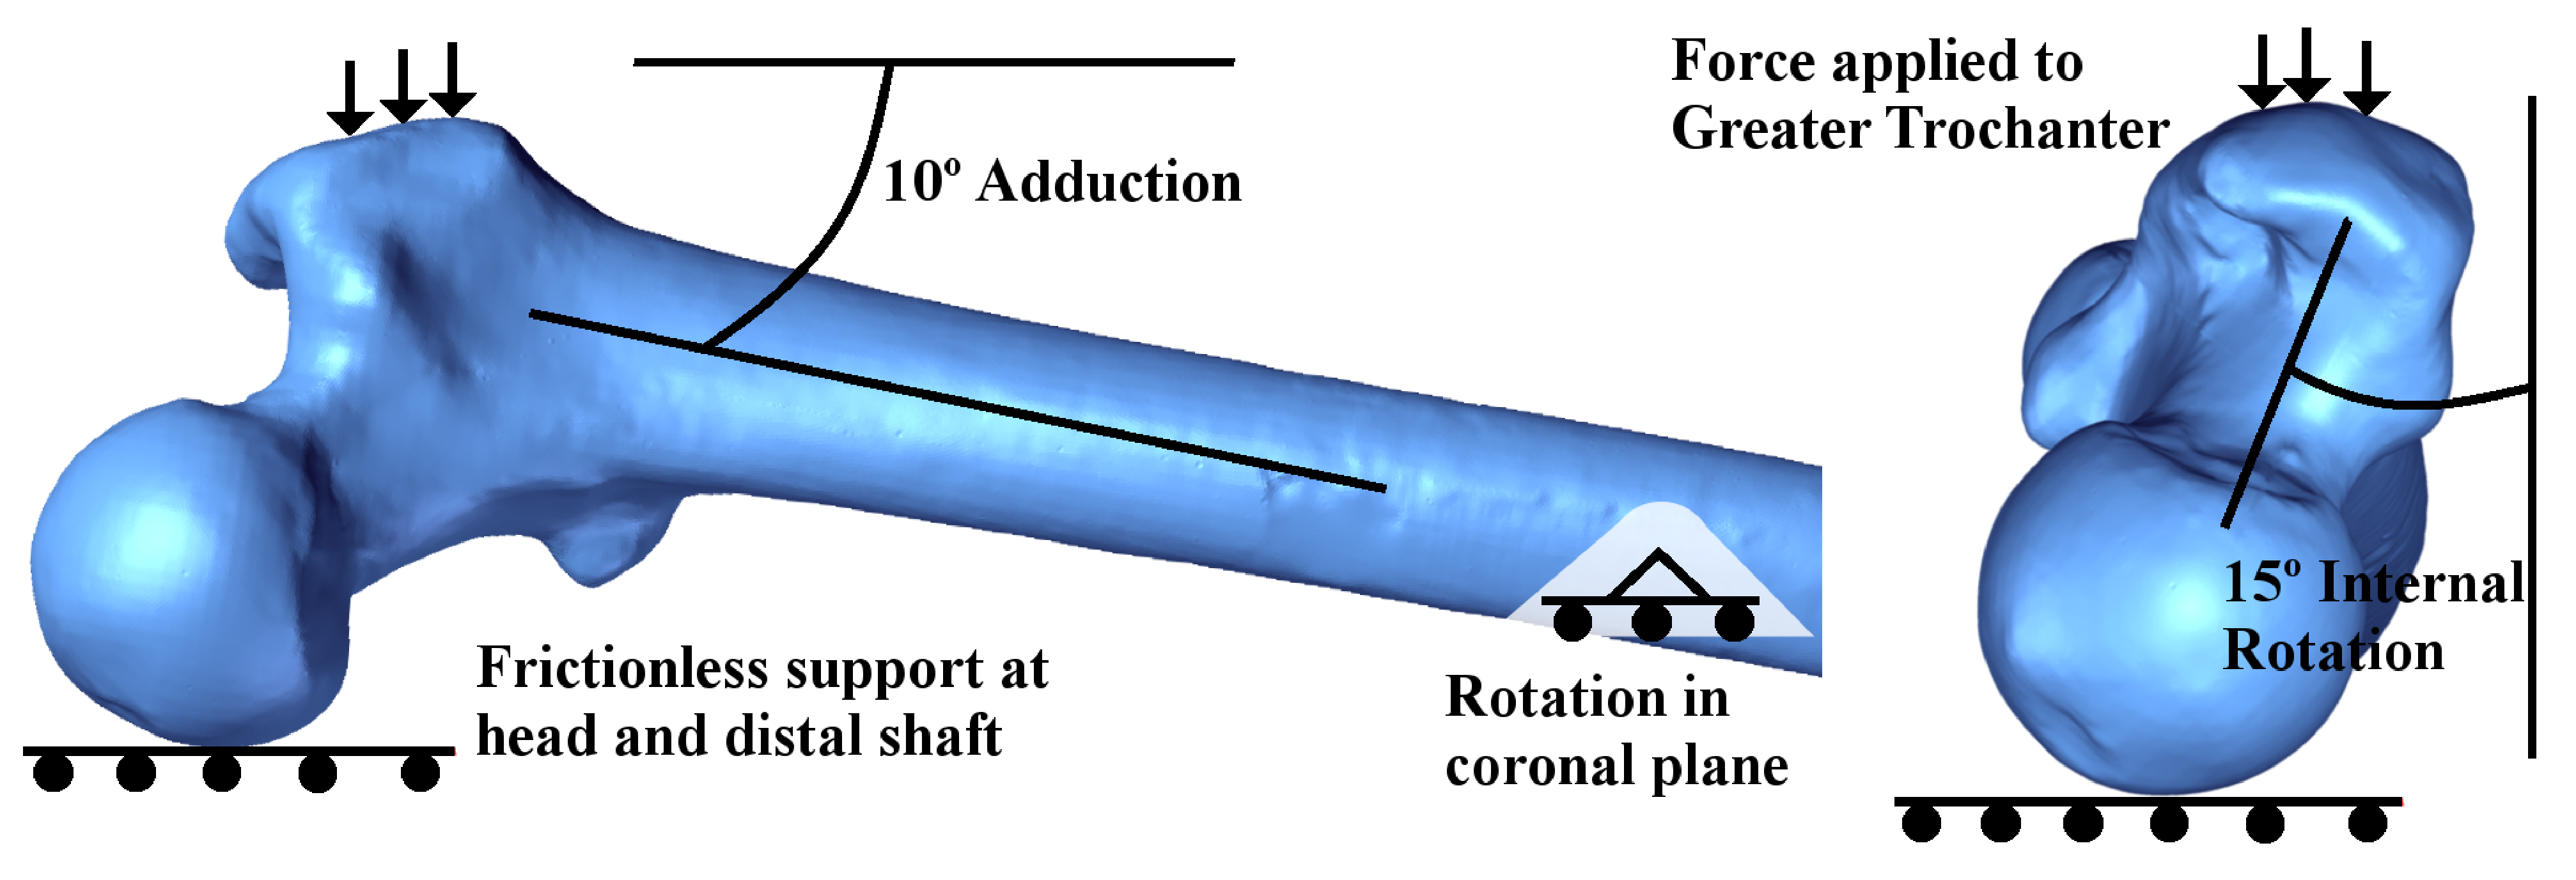
\includegraphics[width=1\linewidth]{./intro/Figures/FEM_Constraints}
	\caption[Proximal femur loading and orientation constraints]{\textbf{Constraints and orientation of the proximal femur in laboratory testing. Anterior view (left) and superior view (right).} Graphic \copyright Seth Gilchrist, 2013.}
	\label{fig:constraint_orient}
\end{figure}
	
\subsection{Application of force}
\label{sec:intro_understanding_modelling_lab_force}
The method used to apply force to the bone in a laboratory model can influence fracture because it changes loading and displacement rates.
The resulting loading and displacement rates could, in turn, affect the material properties due to the viscoelastic nature of bone, as discussed in~\S\ref{sec:intro_boneBehaviour}.
As the material in the bone fails, a progressive change in loading path and strain rates could then change the mechanics of the failure as discussed in~\S\ref{sec:intro_boneStrength}, such that erroneous force application could change the resulting failure and fracture patterns.

Force is applied to the lab models using either a constant displacement rate, or in some cases, an impact using a dropped mass.
\Citet{backman_proximal_1957} did not see any difference in fracture patterns between bones loaded at a constant compression rate and those loaded by impact.
Additionally, work examining bone tissue response to loading rate~\citep{carter_bone_1976, currey_effects_1975} showed a weak influence of strain rate to mechanical properties.
These two facts led early hip fracture researchers to use low, constant displacement rate at the greater trochanter~\citep{lotz_use_1990}.

Knowing that bone material is viscoelastic, researchers saw the application of the force using a low displacement rate as a possible weakness of the testing method, leading them to investigate the effects of increasing the displacement rates.
\Citet{courtney_effects_1994} used a materials testing machine to apply constant-rate displacements on donor-match pairs of femurs at 2~and 100~\ac{mm}/\ac{s}.
This work showed that increasing the displacement rate significantly increased the stiffness and energy to failure, and moderately increased the load to fracture.
In the years following this paper, many experiments have been carried out using a constant displacement rate of 100~\ac{mm}/\ac{s} at the greater trochanter~\citep{de_bakker_during_2009, manske_cortical_2008, manske_femoral_2006, sutter_biomechanical_2010}.
Displacement rate was not seen to influence positive correlation with \ac{abmd}, and results from lower rate tests are still considered valid.
Interestingly, the effects seen by \citet{courtney_effects_1994} were much stronger than would be predicted by isolated bone testing alone (\S\ref{sec:intro_boneBehaviour}).
If one assumes that the strain rate is directly proportional to displacement rate, one might expect an increase in displacement rate of 50x to increase the stiffness by approximately 20-30\%, and likely decrease the energy to failure~\citep{mcelhaney_dynamic_1966, carter_compressive_1977, linde_mechanical_1991}.
\Citet{courtney_effects_1994} found that femurs compressed at high displacement rates were approximately 100\% stiffer than those compressed at low rate and absorbed more energy to fracture, further illustrating the complexity in deriving organ level behaviours based on the behaviour of tissues.

Not all research has been conducted using constant velocity.
Three researchers~\citep{backman_proximal_1957, weber_proximal_1992, okuizumi_effect_1998} have utilized impacts to apply loads to specimens.
\citet{backman_proximal_1957} showed no difference in fracture pattern between impact and constant displacement rate loading.
However, his experiments were performed on dried femora and lacked the ability to accurately measure force or displacement, so were unable to evaluate biomechanical response to the different loadings.
\citet{weber_proximal_1992} used an impact at 4~\ac{m}/\ac{s} with an energy of 360~J (approximately 2-3x the current estimated energy in a fall to the side~\citep{robinovitch_distribution_1997, feldman_reducing_2007}) and found similar results to \citet{courtney_effects_1994}, in which all mechanical metrics increased as displacement rate increased.
\citet{okuizumi_effect_1998} investigated the effects of different hip protectors on the failure strength of proximal femurs using a dropped mass.
However, the impact mass, velocity and energy were not biomechanically justified and not compared to more traditional methods, so the influence of this protocol on the outcome is unknown.

\subsection{Lessons learned from laboratory models}
\label{sec:intro_understanding_modelling_lab_results}
As mentioned in \S\ref{sec:intro_understanding_tolerance}, once a laboratory model is validated for a certain scenario it can be used to examine any independent variable such as tissue displacement, force response, or yes/no injury classification.
Taking advantage of this aspect of laboratory models, many different properties of the proximal femur loaded in the fall configuration have been examined (Table \ref{tab:model_results}).

\let\thempfootnote\thefootnote
\def\arraystretch{1.5}

\begin{table}
\caption[Laboratory model results summary]{Important results and references for laboratory tests.}
\label{tab:model_results}
\begin{tabularx}{\textwidth}{l X p{4cm}}
\toprule
Aspect & Influence & Reference(s) \\ \midrule

Orientation & Increased internal rotation lowers ultimate strength. Standing vs.\ falling orientation changes strength, but ratio of the strengths depend on the definitions of ``standing" and ``falling". & \citep{pinilla_impact_1996, turner_biomechanics_2005, keyak_relationships_2000, lochmuller_mechanical_2002} \newline \citep{ford_effect_1996, keyak_effect_2001}\footnotemark  \\

Compression rate & Increased compression rate leads to increased stiffness, ultimate load and energy to failure. & \citep{courtney_effects_1994, weber_proximal_1992, okuizumi_effect_1998, backman_proximal_1957} \\

\ac{bmd} and \ac{abmd} & Higher \ac{bmd} leads to increased strength. & \citep{boehm_prediction_2008, bouxsein_ultrasound_1995, cheng_prediction_1998, cheng_assessment_1997, lochmuller_mechanical_2002, lotz_use_1990, roberts_comparison_2010, manske_cortical_2008, manske_femoral_2006, pulkkinen_experimental_2008, leichter_optical_2001} \\

Cancellous bone & Cancellous bone important in a fall, less so in standing. & \citep{manske_femoral_2006, manske_cortical_2008, holzer_hip_2009, pulkkinen_experimental_2008, blain_cortical_2008} \\

Cortical bone & Thin cortex is indicative of reduced strength. & \citep{lochmuller_mechanical_2002, manske_femoral_2006, manske_cortical_2008, crabtree_intracapsular_2001, de_bakker_during_2009, de_bakker_hip_2006, mayhew_relation_2005, blain_cortical_2008} \\

Age & Increased age relates to decreased \ac{bmd} and strength. & \citep{courtney_effects_1994, courtney_age-related_1995} \\

Side & Side-to-side strength in the same person differs on average by 19\% and 16\% for women and men, respectively. & \citep{eckstein_reproducibility_2004} \\

Geometry & Certain geometrical features, such as a long or narrow femoral neck, relate to increased fracture risk. & \citep{cheng_assessment_1997} \\

Failure location & Failure typically initiates in the anterior-superior neck. & \citep{de_bakker_hip_2006, de_bakker_during_2009} \\

Femoroplasty & Augmentation by femoroplasty (\ac{ie}, injection of bone cement to strengthen cancellous bone) increases strength of osteoporotic femurs, but makes revision surgery difficult or impossible. & \citep{heini_femoroplasty-augmentation_2004, beckmann_femoroplasty--augmentation_2007, sutter_biomechanical_2010, de_bakker_hip_2006} \\

\bottomrule
\end{tabularx}
\footnotetext[1]{Computational studies}
\end{table}

\def\arraystretch{1}

Orientation has been shown to influence femoral strength, with an increased internal rotation relating to a decrease in the strength of the specimen~\citep{pinilla_impact_1996, ford_effect_1996}.
Changing the orientation from a standing model to a side impact model showed a difference in one study~\citep{keyak_relationships_2000}, but not a second one~\citep{lochmuller_mechanical_2002}.
However, these two studies used different orientations to model a side impact, with~\citet{keyak_relationships_2000} using a rather extreme neck internal rotation of 70$^\circ$, which would be predicted to significantly lower the strength of the specimens~\citep{pinilla_impact_1996, ford_effect_1996, keyak_effect_2001, ford_effect_1996}.
	
\ac{bmd} has been included as a variable in many tests, and the data have consistently shown that a higher \ac{bmd} (or \ac{abmd}) leads to an increase in stiffness and ultimate load.

The independent roles of cancellous and cortical bone are known to some degree, but their relative roles are a bit more difficult to determine.
Cancellous bone has been shown to be important in a fall~\citep{manske_femoral_2006, manske_cortical_2008, pulkkinen_experimental_2008}, and less important in standing strength~\citep{holzer_hip_2009}.
Researchers who have compared the relative roles of cancellous and cortical bone in failure scenarios have shown that both have important roles to play, with relative importance varying by failure location~\citep{manske_cortical_2008, pulkkinen_experimental_2008}.

A decrease in strength of specimens loaded in a fall configuration has been shown to be correlated with increasing age; however that change was concurrent with a decrease in \ac{bmd}, which may have accounted for the decrease in strength~\citep{courtney_age-related_1995, courtney_effects_1994}.

Side-to-side strength in the same donor was seen to be  19~($\pm$13)\% (mean~($\pm$\ac{sd})) different in females and 16~($\pm$12)\% different in males~\citep{eckstein_reproducibility_2004}.
This result is important when considering the results of many of the comparative studies listed in Table \ref{tab:model_results}, because results from those studies were often analysed using matched-pairs statistics on donor-matched pairs of femurs.
\citet{eckstein_reproducibility_2004} showed that matched-pairs statistics on donor-matched (left \ac{vs} right) femurs is likely insufficient for statistical significance, as there is considerable variability in strength that is unexplained by \ac{bmd}.

Geometry has been thought to be a promising clinical screening tool, as it can be evaluated using planar x-rays.
As such, it has been predominately studied using clinical methods~\citep{dincel_association_2008, el-kaissi_femoral_2005, faulkner_simple_1993, wang_women_2009}.
Femoral neck length, measured from the medial head to the lateral cortex of the greater trochanter, shows the highest correlation with fracture load~\citep{cheng_assessment_1997}, however this correlation is much lower than that of \ac{bmd} with fracture load.
Clinical evaluations showed that femoral neck length, and hip axis length (which is defined as the distance from the medial border of the pelvis, adjacent to the acetabulum, to the lateral cortex of the greater trochanter along the femoral neck) both correlate with hip fracture risk, but are most powerful when used in conjunction with \ac{bmd}~\citep{faulkner_simple_1993, dincel_association_2008}.

Failure location has been experimentally confirmed in only one study~\citep{de_bakker_during_2009} (and an associated thesis~\citep{de_bakker_hip_2006}).
Fractures were seen to typically originate in the superior or anterior femoral neck, regardless of fracture type (\ac{eg}, cervical or trochanteric).
That said, trochanteric fractures appeared to originated in the lateral neck, whereas neck fractures originated in the sub-capital region.

Femoroplasty is a technique in which \ac{pmma} (\ac{aka}\ bone cement) is injected into the proximal femur as a way to reinforce the senile trabecular structure.
Studies on femoroplasty have shown that it significantly increases strength and energy to failure~\citep{de_bakker_hip_2006, heini_femoroplasty-augmentation_2004, sutter_biomechanical_2010}.
These benefits are currently outweighed by complications in dealing with large quantities of \ac{pmma}, which include the highly exothermic reaction as it sets~\citep{de_bakker_hip_2006, heini_femoroplasty-augmentation_2004}, and difficulty with revision surgery due to the hardness of the material~\citep{beckmann_femoroplasty--augmentation_2007}.
	
\subsection{Limitations of laboratory models}
\label{sec:intro_understanding_modelling_lab_limits}
The data gathered in laboratory experiments are of great importance to an understanding how the proximal femur behaves during a fall to the side.
However, there are limitations to the current laboratory models which must be understood in order to apply the results.
One of the principal limitations is the lack of a biofidelic, dynamic model of the fall.
Previously published models attempt to apply loads representative of a fall by applying a constant-rate compression of 100~\ac{mm}/\ac{s}.
This compression rate has never been validated as a reasonable value, and therefore must be taken with caution -- especially given the influence it has on the behaviour of the bone.

The majority of the models use materials testing machines to apply compression to the lateral trochanter, and continue compression until fracture is attained.
This method of creating fractures ignores the fact that the bone is not loaded in constant displacement rate.
Rather, it is loaded by the inertia of a falling mass (\ac{ie}, the body) and mediated by deformable elements (\ac{eg}, pelvis, skin and fat).
This means that the loading conditions (such as displacement rate) will be a function of the fall characteristics and the properties of the proximal femur itself. 
Additionally, the energy of the mass in the fall is limited and fracture is not guaranteed.
In fact, fracture is seen in only $\sim$5\% of real-world falls in the elderly~\citep{masud_epidemiology_2001, nachreiner_circumstances_2007}.

The results of the laboratory models are also at odds with the epidemiology.
Laboratory fracture models have failed to identify any significant predictor of fracture besides \ac{bmd}.
Studies of fractures in the general population show a considerable overlap of \acp{bmd} between fracture and non-fracture patients~\citep{greenspan_fall_1994, faulkner_simple_1993}.
As few as 22\% of hip fractures patients have \acp{bmd} that would classify as osteoporotic, and 42\% that would classify as osteopenic or osteoporotic~\citep{stone_bmd_2003}.
This could be due to the use of ultimate load as the criteria for fracture resilience, and also may be influenced by the constant displacement rate, rather than inertial impact, testing method.		

\subsection{Summary}
\label{sec:intro_understanding_modelling_lab_summary}
Laboratory models of hip fracture have been used extensively to determine the influence of different aspects of the proximal femur on its strength.
The primary focus of the modelling has been to understand the strength in a fall to the side, and in this respect researchers have developed methods that have shown the influence of many physical characteristics.
Even with all of this effort and knowledge, there are still gaps between what is being modelled and the real world.
A potential next step in laboratory testing is to refine the model of a fall to the side, increasing its biofidelity to allow researchers to understand the inputs and results of real world falls.

\section{Computer models}
\label{sec:intro_understanding_modelling_comp}
Computer models are performed using the \acf{fe} and \acf{mbd} techniques.
Most of the information about the mechanism of hip fracture gleaned from computer models has come from \ac{fe} models because they are capable of providing stresses, strains and potential failure locations.
This section focuses on the contributions and limitations of \ac{fe} models.
There have been few \ac{mbd} models that have provided insight into hip fracture, focusing primarily on determining the fall conditions, which are discussed more thoroughly in Chapter \ref{ch:fall_sim_design}.

\subsection{Contributions of \acs*{fe} models}
\label{sec:intro_understanding_modelling_comp_use}
\ac{fe} models are, in most cases, based on a laboratory model that can be used as a validation.
Once an \ac{fe} model is validated, it can be used to examine a number of different aspects of the failure event, including the role of soft tissue~\citep{majumder_simulation_2007}, fall modelling~\citep{majumder_effects_2008}, non-invasive strength estimation for an arbitrary bone~\citep{keaveny_femoral_2008, srinivasan_relationship_2011, viceconti_automatic_2004}, and fracture risk estimation~\citep{orwoll_finite_2009, srinivasan_relationship_2011, tanck_predictive_2009}.

In addition to all of these uses, \ac{fe} models have been used to understand the fracture itself.
Multiple researchers have used \ac{fe} models to estimate the location where fractures begin and what conditions lead to fracture~\citep{keyak_prediction_2001, keyak_prediction_2000, keyak_prediction_1998, nawathe_microstructural_2013, lotz_fracture_1991, lotz_fracture_1991-1, lotz_stress_1995, ota_fracture_1999, tanck_predictive_2009, verhulp_comparison_2006, verhulp_load_2008, bryan_use_2009}.
Data from these models have increased the understanding of the conditions in the femur leading up to fracture, but there are significant limitations to the models that can affect interpretation of their results.
	
\subsection{Limitations of \acs*{fe} models}
A primary limitation of \ac{fe} models relates to the experimental models used to determine their validity.
As discussed in \S\ref{sec:intro_understanding_modelling_lab}, the displacement rate used to load a proximal femur can influence its mechanical and failure behaviours.
It is thought that these changes in organ level behaviour originate from changes at the bone material level (see~\S\ref{sec:intro_boneBehaviour} and~\S\ref{sec:intro_boneStrength}).
The experiment used to validate an \ac{fe} model should replicate the boundary and loading conditions applied in the model, and also have the similar material properties as those applied in the model.
Failing to meet these requirements can lead to validation uncertainty.

The material properties applied to a model are often determined from tissue level tests conducted at low strain rate, while the validation experiment is an organ level test conducted at high displacement rate (\ac{eg}, 100~mm/s).
As a result, it is possible that significant differences exist in bone properties in the tissue and organ level tests.
If the \ac{fe} model agrees with the organ level test, it could be due to an error in the model (such as an inappropriate constraint), rather than accurate representation of the experiment.

It is possible that the displacement rate does not affect the desired outcome variable, making the selection of a validation experiment essentially arbitrary.
However, if there is a dependence on experimental method, \ac{fe} researchers must be sure to select material properties that are in agreement with their validation experiments.
Currently, there is no standard for what experiment should be used to validate a given \ac{fe} outcome variable and therefore special attention should be paid to possible interplay between materials definitions and model validation.

In addition to validation challenges, selecting appropriate material properties for the \ac{fe} model can be complicated.
As we have seen in previous sections, bone is a highly complex material at all length scales, making simplifications for computational applications necessary.
The majority of \ac{fe} models use relatively simple material definitions that lack the anisotropy and viscoelasticity discussed in \S\ref{sec:intro_boneBehaviour}.
This lack of fidelity in the material model may influence how load is transferred and how failure is determined given that ultimate strain is a function of strain rate.
Additionally, they use a single phase, neglecting the flow of bone marrow, which has been shown to be important at high strain rates~\citep{carter_compressive_1977}.
A final limitation of the material definitions in current \ac{fe} models is the use of a highly simplified post yield behaviour model.
After yield, bone behaviour is dependent on the bone type~\citep{hayes_biomechanics_1997}, loading direction~\citep{hansen_effect_2008}, and loading rate~\citep{hansen_effect_2008, kulin_effects_2011, kulin_loading_2011}, making computational modelling very difficult.
There are efforts to address this final limitation using plastic material models for post yield behaviour~\citep{derikx_implementation_2011, verhulp_micro-finite_2008, bayraktar_comparison_2004}.
However, those models are still simple, modelling both tension and compression in the same manner, and lacking the non-linearity of post-yield strain with strain rate seen in the bone core tests described in \S\ref{sec:intro_boneStrength}~\citep{derikx_implementation_2011, bayraktar_comparison_2004}.

Another limitation of \ac{fe} models of biological systems is that they are deterministic in nature, \ac{ie}, each model has only one solution, even though there are many probable outcomes for a given loading scenario in the physiological situation.
This limitation has been addressed using Monte Carlo simulations for material and geometry, which provide a distribution of strains or stresses for a given element, in a given loading scenario~\citep{bryan_use_2009, taddei_finite-element_2006, laz_incorporating_2007}.
These statistical simulations attempt to address the uncertainly regarding material properties and geometry, but do not address uncertainly in fluid flow, or changes in material properties due to deformation, strain rate, or loading direction.
	
One final but important note relating to the interpretation of the results of \ac{fe} models is that many predict failure in the cancellous bone~\citep{bryan_use_2009, keyak_prediction_2001, keyak_prediction_2000, keyak_prediction_1998, lotz_fracture_1991, lotz_stress_1995, nawathe_microstructural_2013, verhulp_comparison_2006, verhulp_load_2008}.
This result is intriguing, but one must remember computational models are only valid for output variables that have been validated.
Since the deformation of the cancellous bone cannot be directly measured in experimental tests, it has never been validated, and this necessarily limits the scientific reliability of these data.
To fully trust the results that are given for internal strains, a method needs to be devised and implemented to experimentally determine the actual internal deformations for comparison and validation.

\subsection{Applications of models to fracture prevention}
\label{sec:intro_understanding_application}
Modelling results have been applied to the development of a number of different biomechanical technologies that are intended to prevent hip fracture.
The most advanced in terms of development and assessment are hip protectors, which are soft or hard pads that are positioned over the greater trochanters using special undergarments.
Hip protectors have been shown to decrease the impact force~\citep{choi_effect_2010,laing_force_2008, van_schoor_biomechanical_2006}, but have not proven effective in the real-world~\citep{kiel_efficacy_2007, parker_effectiveness_2006}.

Another more recent development is compliant flooring, which modifies the landing surface in order to decrease the impact force~\citep{laing_effect_2006, li_comparison_2013}.
This technology is currently in the development and proving stage~\citep{clinicaltrials.gov_flooring_2012}, but shows promise as a passive strategy to protect individuals against fracture in a way that is effective immediately and not compromised by lack of compliance -- the two main problems with pharmacological remedies (which can take years to become effective) and hip protectors (which are often not worn at the time of a fracture).

Both of these technologies use data from modelling of hip fracture to determine the target maximum forces in their simulated falls.
Some tests also use knowledge of where fractures are likely to occur to determine effectiveness for a particular injury~\citep{laing_force_2008}.

\chapter{Objective and research questions}
\label{sec:intro_goals}
The objective of this thesis is to quantitatively compare the mechanical and failure behaviours of hip fracture in constant displacement rate loading with the behaviours in impact fall simulation.
Specifically, this research will determine if experimental constant displacement rate models of hip fracture produce force-displacement, strain, failure and fracture results that are similar to those observed in impact fall simulation.
Any differences observed in the behaviours of the bones between these two experimental models will inform a decision matrix.
This matrix can be used as a guide by \textit{ex vivo} and \ac{fe} modellers to select the most appropriate experiment for their outcome variables or validation needs.

\section{Research questions}
\label{sec:intro_goals_questions}
In pursuit of these objectives, I have identified three research questions:
\begin{enumerate}
\item Does the force-displacement mechanical response of a proximal femur differ when it is loaded using constant displacement rates \ac{vs} impact fall simulation?
\item Does the surface strain field of the proximal femur differ when it is loaded using constant displacement rates \ac{vs} impact fall simulation?
\item Do the locations of initial failure and final fracture change when the proximal femur is loaded using constant displacement rates \ac{vs} impact fall simulation?
\end{enumerate}

\section{Method of investigation}
\label{sec:intro_method}
To answer the research questions, an inertially driven fall simulator with elements modelling the body, pelvis, and soft tissues over the greater trochanter has been built.
Its design and development are discussed in Chapter \ref{ch:fall_sim_design}.
This fall simulator was used in conjunction with a materials testing machine to determine if the mechanical, strain and failure  behaviours of the proximal femur are similar or divergent between the quasi-static and impact loading methods.

\subsection[Force-displacement behaviour]{Does the force-displacement behaviour differ between constant displacement rate and impact fall simulation testing?}
\label{sec:intro_method_behave}
This question was addressed by comparing the sub-failure, force-displacement response of proximal femurs loaded using quasi-static, constant displacement rates in a materials testing machine and the response of the same femurs loaded to failure in the impact fall simulator.
Single specimens were loaded to 50\% of their \ac{abmd} predicted failure load in a materials testing machine, and the behavioural metrics of force, displacement, stiffness, and energy to maximum applied load were measured.
The same bones were then transferred to the impact fall simulator and loaded to failure.
The same metrics measured in the quasi-static tests were measured in the fall simulation tests and compared to the quasi-static results at the the maximum load applied in the materials testing machine.
This research is presented in Chapter~\ref{ch:behave_fail}.

\subsection[Strain behaviour]{Does the surface strain differ between constant displacement rate and impact fall simulation testing?}
\label{sec:intro_method_fail}
This question was addressed using stereo \acf{dic} of the anterior-superior surface of the femoral neck. % during quasi-static, constant displacement rate loading in a materials testing machine and impact fall simulation.
Stereo, \ac{3d} \ac{dic} data were collected on the anterior-superior femoral neck of single specimens loaded to 50\% of their \ac{abmd} predicted failure loads in a materials testing machine, followed by loading to failure in the impact fall simulator.
The \ac{3d} surface profiles measured by the \ac{dic} software were aligned, and the minimum principal strains on the surfaces were compared to determine if there was a difference in strain magnitude or distribution between the two loading protocols.
This work is presented in Chapter~\ref{ch:fracture}.

\subsection[Failure behaviour]{Do the failure locations and final fracture types differ between constant displacement rate and impact fall simulation testing?}
\label{sec:intro_method_fracture}
This question was addressed using two groups of specimens, one group loaded to failure in a materials testing machine under quasi-static, constant displacement rates and another group loaded to failure in the impact fall simulator.
Fracture locations were determined from high-speed videos of the experiments and final fracture types were classified by an orthopaedic surgeon and compared between the two groups.
This research is presented in Chapter~\ref{ch:fracture}.

%    Main body
%% This is the impactor chapter for my UBC PhD Dissertation
%% The parent document is called thesis.tex

\chapter{Design of a fall simulator}
\label{ch:fall_sim_design}
Before the behaviour of the proximal in a simulated fall can be compared to the behaviour in quasi-static loading, a validated impact fall simulator must be developed.
Impact fall simulation has been used by the hip protector design community for many years, however, the particular requirements of testing human material makes adaptation of a pre-existing fall simulator impossible.
In this chapter, the rational, design and justification for a drop tower apparatus that simulates a human fall to the side from standing, is presented.

This chapter was published as a peer reviewed paper in ASME Journal of Biomechanical Engineering~\citep{gilchrist_development_2013} and is reprinted here with permission.

\section{Introduction}
\label{sec:fall_sim_design_intro}
Hip fracture is a devastating injury associated with high morbidity and mortality in the elderly as well as high treatment cost~\citep{braithwaite_estimating_2003, forsen_survival_1999,wiktorowicz_economic_2001}.
In order to prevent or improve treatment of these injuries, researchers have conducted extensively laboratory studies, with previous \textit{ex vivo} models of hip fracture establishing the role of posture~\citep{pinilla_impact_1996, ford_effect_1996}, compression rate~\citep{courtney_effects_1994, weber_proximal_1992}, and bone density~\citep{lotz_use_1990, lochmuller_mechanical_2002, manske_cortical_2008} in the strength of the femur.
Bone density has been shown to correlate to the strength of a proximal femur loaded in a fall posture, and constant compression rates ranging from 0.7~\ac{mm}/\ac{s}~ to 100~\ac{mm}/\ac{s}~\citep{courtney_effects_1994, weber_proximal_1992} have been used to prove that the proximal femur's mechanical properties depend on compression rate magnitude.

In all of the previous studies, tests were conducted using materials testing machines to apply loads to either the head or lateral trochanter of the femur~\citep{boehm_prediction_2008, courtney_effects_1994, de_bakker_during_2009, lochmuller_mechanical_2002, lotz_use_1990, manske_cortical_2008, roberts_comparison_2010, weber_proximal_1992, keyak_relationships_2000}.
While compression rate varied from experiment to experiment, in each case it was fixed and constant throughout testing, and the final result was fracture of the bone.
Only two researchers have conducted tests at high compression rates~\citep{weber_proximal_1992, backman_proximal_1957}, potentially representative of rates that would be experienced in a fall, but they tested the femur in isolation, neglecting the influence of surrounding tissues and structures.

Falls are by definition dynamic, inertia-driven events in which compression rates are not constant, and in some portions of the event may be as high as 3000~\ac{mm}/\ac{s}~\citep{feldman_reducing_2007}, although in individuals that are able to react quickly, fall speeds are often slowed due to an extended hand or other protective action~\citep{van_den_kroonenberg_dynamic_1995, feldman_reducing_2007}.
Additionally, fracture is not prescribed in a fall, with only $ \sim $5\% of falls resulting in fracture~\citep{nachreiner_circumstances_2007}.
In a fall to the side, the compression rate of the proximal femur is dependent on the contact velocity with the ground, properties of the overlying soft tissue, stiffness and mass of the pelvis, mass of the body, and the stiffness of the proximal femur itself.
The stiffness of the proximal femur is of primary importance to its resulting behaviour and is itself a function of compression (strain) rate~\citep{mcelhaney_dynamic_1966, crowninshield_response_1974, saha_instrumented_1974, currey_effects_1975, carter_bone_1976, robertson_compressive_1978, linde_mechanical_1991, courtney_effects_1994, pithioux_comparison_2004, hansen_effect_2008, zioupos_microcracking_2008, weber_proximal_1992}.
The recursive nature of this process means that the compression rate of the femur will not be constant during the impact event and in only a subset of bones will result in fracture.
Modelling the compression rate of the lateral femur as a constant, and deterministically imposing fracture, is a significant limitation of the previous experiments, and may limit their ability to inform researchers about the mechanics of the fracture and how to identify the specific bones that are susceptible to fracture.

In addition to these biomechanical observations, epidemiological research has shown that a discrepancy exists between what is expected from lab results and what is seen in the general population.
Lab and epidemiology results~\citep{borissova_femoral_2011, cauley_risk_2009} have shown that bone density is an important factor that is correlated to fracture load, but we also see that more than two-thirds of fractures occur outside the low bone density population~\citep{stone_bmd_2003, siris_bone_2004, greenspan_fall_1994}
This indicates that other factors (\ac{eg}, structural) may be involved~\citep{singh_changes_1970, naylor_use_2012, bouxsein_bone_2003}.

No researchers have explicitly modelled the fall and observed the resulting bone behaviour, which would dependent recursively on both fall mechanics and the bone's response, as described above.
Understanding these behaviours may illuminate potential screening targets, helping inform and improve biomechanical (\ac{eg}, hip protectors) and clinical (\ac{eg}, pharmaceutical) hip fracture prevention.
Thus, in an effort to bridge the gap between current \textit{ex vivo} hip fracture models and \textit{in vivo} fractures, this research comprises two related aims: a) develop an impact-based testing apparatus to model a physiological fall to the side, including representations of the surrounding anatomic structures; b) validate quantitative methods for analysing loading mechanics using high speed imaging and surface strain analysis.

The mechanics of hip fracture are influenced by the structures and tissues (referred to as \emph{elements}) surrounding the femur.
These elements are, on the medial side, the pelvis and body, and on the lateral side, the soft tissue over the trochanter.
Previous efforts have been made to understand the behaviour of these elements in isolation, and in some cases researchers have incorporated them into tests to evaluate the effectiveness of biomechanical devices such as hip protectors or compliant flooring~\citep{robinovitch_hip_2009, laing_force_2008,laing_effect_2006}.
In the following sections, research surrounding each element will be considered and representative properties will be chosen for inclusion in our laboratory model.
Finally, the behaviour of the model during a simulated fall will be compared to the behaviour of published human volunteer tests to evaluate the biofidelity of the apparatus.

In addition to the above device development, a quantitative method of evaluating the strain on the bone surface will be validated.
Researchers have traditionally used strain gauges to evaluate the strain state of the proximal femur during loading to fracture~\citep{cristofolini_vitro_2007}.
It is known from finite element analyses~\citep{verhulp_comparison_2006} and from research on the experimental error of strain gauges~\citep{cristofolini_vitro_1997} that strain gradients on bones can be high.
This has two primary consequences for their use for strain measurement: 1) it is difficult to compare two models of the same event (\ac{eg}, comparing a fracture experiment to a subject-specific finite element model), and 2) placement of gauges in locations where meaningful strain is "guaranteed" to occur is impossible.
In an experiment complementary to the development of the fall simulator, we will directly compare strain measurements from \acf{dic}, which is a method for full field strain measurement, to the gold standard strain rosette.
Our goal is to validate the use of \ac{dic} for measurement of strain on the surface of a proximal femur so that future experiments can use it in lieu of strain rosettes.

\section{Materials and methods}
\label{sec:fall_sim_design_methods}
A drop tower-based fall simulation apparatus was developed and its loading mechanics were compared to the response of volunteer, as well as human cadaver hip and pelvis tests.
In addition to the apparatus development, low compression rate, sub-failure tests were conducted on human bone specimens to validate the use of digital image correlation for surface strain measurement on the femoral neck.
These techniques will be used in future experiments to determine the loading and fracture mechanics of human proximal femora loaded in a fall configuration.

	\subsection{Fall simulator apparatus}
	\label{sec:fall_sim_design_methods_apparatus}
	Due to the dynamic nature of a fall to the side, the tissues and structures surrounding the proximal femur must be included for accurate biofidelic modelling.
	These structures are, on the lateral side of the femur, skin and soft tissue over the trochanter, and on the medial side, the pelvis and body.
	The biological scenario was simplified to a lumped parameter model (Figure \ref{fig:MassModel}) which was characterized using a state-of-the-art plastic bone surrogate for consistency (3rd Gen.\ Large Femur, Sawbones\texttrademark, Vashon, WA).
	The following sections contain a literature review and justification for the properties selected for each element.
	
	\begin{figure}
		\centering
		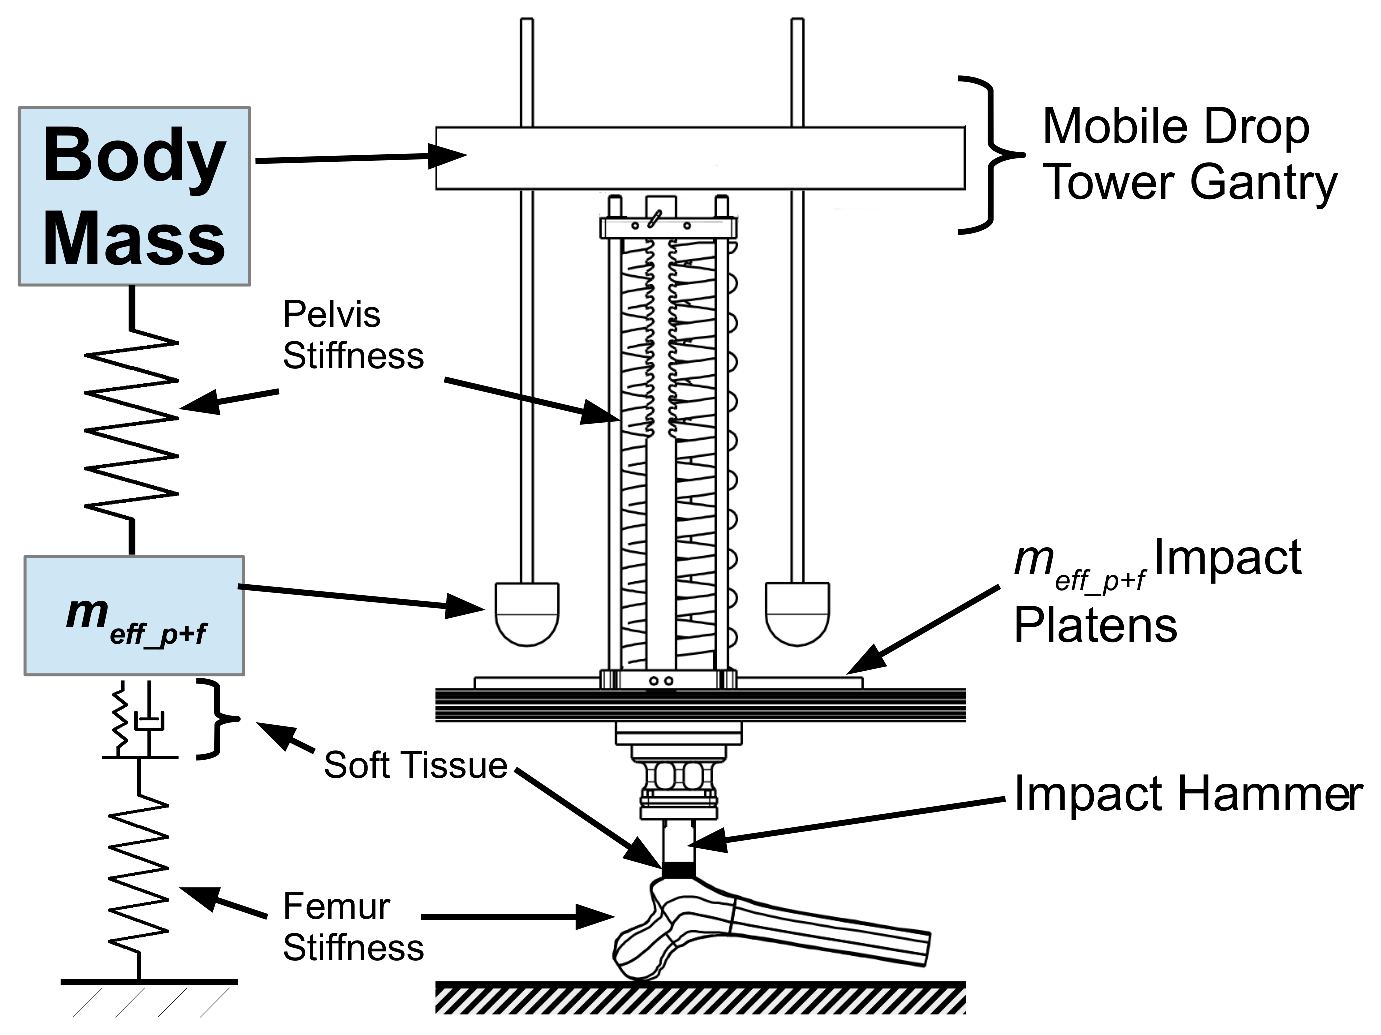
\includegraphics[width=.7\linewidth]{./impactor/figures/MassModel.eps}
		\caption[Schematic of the fall simulator]{\textbf{Schematic of the fall simulator showing the mass and spring of structures that influence loading a fall to the side.
		$m_{eff\_p+f}$ is the effective mass of the lateral pelvis and femur.}}
		\label{fig:MassModel}
	\end{figure}

		\subsubsection{Effective body mass}
		\label{sec:fall_sim_design_methods_apparatus_body}
		The selection of the body mass determines (along with the pelvis and soft tissue stiffnesses) the peak force and (along with the impact velocity) the energy delivered during the impact.
		Body habitus, measured using BMI, has been shown to correlate negatively with hip fracture risk~\citep{orwoll_finite_2009, parker_association_2008, nguyen_abdominal_2005, nguyen_identification_2005, minns_are_2007}, indicating that increased body mass can be protective.
		There is, however, also some evidence to the contrary, especially that very high body mass can increase fracture risk~\citep{nielson_bmi_2011}.
		To quantify how body mass influences the loading parameters during a fall, researchers have mathematically modelled falls using link assemblies~\citep{van_den_kroonenberg_dynamic_1995}, and performed pelvis drop experiments on young, university-student volunteers~\citep{robinovitch_prediction_1991, laing_characterizing_2010}.
		
		In a fall to the side the effective body mass impacting the trochanter is less than the total body mass of the person falling.
		Conceptually, this is because some of the body mass would be supported by the feet and lower extremities.
		Experimentalists and computational modellers have put this so-called \emph{effective body mass} at approximately half body weight~\citep{van_den_kroonenberg_dynamic_1995, robinovitch_prediction_1991}.
		Additionally, direct measurement of the effective mass in young volunteers has provided a range of 24.1--50~\ac{kg}~\citep{robinovitch_prediction_1991, van_den_kroonenberg_dynamic_1995, robinovitch_distribution_1997, laing_force_2008} with a cross-study average for human tests subjects of 31.9~\ac{kg}.
		The cross-study average for the computational models was higher, and more variable depending on the assumptions made in the model.
		The cross-study average of human subjects did not show the same variability due to model design, or dependency on assumptions, and was taken as the value of the effective body mass.
		A value of 32~\ac{kg} was selected for the fall simulator, which is within one standard deviation of 50\% body weight of hip fracture cases~\citep{armstrong_body_2011, orwoll_finite_2009, bouxsein_contribution_2007, nielson_trochanteric_2009}.

		\subsubsection{Effective mass of the femur and lateral pelvis}
		\label{sec:fall_sim_design_methods_apparatus_pelvis}
		The two main mass components that govern the loading of the proximal femur in a fall are: a) the body mass, whose impact is attenuated by the compliance of the pelvis, and the selection of which was discussed above; and b) the mass of the lateral pelvis and proximal femur, whose impact is attenuated only by the compliance of the femur and overlying soft tissue (Figure \ref{fig:MassModel}).
		Previous work on pelvis fracture in automotive, side-impact accidents performed impacts of osteoligamentous pelvises at $\sim$4.5~\ac{m}/\ac{s}~\citep{beason_bone_2003}.
		In these experiments, an impact hammer was instrumented with a load cell and dropped on to the greater trochanter of the femur.
		In the resulting force-time traces a force spike was seen early in the loading history, before deformation of the pelvis started (Figure \ref{fig:CompBeason}).
		This force spike was created by the inertia of the mass close to the impact surface.
		
		To better understand the origin of this pulse, consider that in an impact, the velocity of the impact hammer and the contact point on the object being impacted must become equal, creating a force due to the inertia of the mass near the contact point.
		In the case of a fall to the side, before the pelvis can compress, the proximal femur and lateral pelvis must go from moving 3~\ac{m}/\ac{s}, to being stationary against the ground.
		This happens very quickly, requiring a high acceleration, and creating a force pulse at the interface between the ground and the trochanter.
		This behaviour has been documented in head-first impact studies, where a force pulse is generated as the head is stopped before compression of the neck begins \citep{nightingale_dynamic_1997, saari_cervical_2011}.
		In the fall to the side, as one moves medially from the contact point, the pulse is attenuated due to the compliance of the tissues between the ground and the location under consideration.
		Because they are relatively stiff and close to the impact surface, the lateral trochanter and femoral neck will see a considerable portion of this force pulse.
		Since the magnitude can be quite high, as seen in Figure \ref{fig:CompBeason}, it must be accounted for in the test apparatus.
		Once the velocity of femur and lateral pelvis have gone to zero, force in the proximal femur is generated by the body compressing the pelvis.
		
		The effective combined mass of the lateral pelvis and proximal femur ($m_{(eff\_p+f)}$) during an impact was determined using a momentum analysis of the osteoligamentous pelvis impacts~\citep{beason_bone_2003}.
		The momentum equation is $\int Fdt = m_{(eff\_p+f)}\cdot \varDelta V$ and the desired quantity is the effective mass of the lateral pelvis and femur.
		The force time traces were numerically integrated to determine $\int Fdt$, and optical tracking data from markers attached to the greater trochanter were used to determine $\varDelta V$.
		The quotient of $ \frac{\int Fdt}{\Delta V} $ gave the effective mass of the lateral pelvis and proximal femur in these tests.
		This analysis yielded an effective mass (average $\pm$ \ac{sd}) of 0.97$\pm$0.52~\ac{kg}.
		
		\begin{figure}
			\centering
			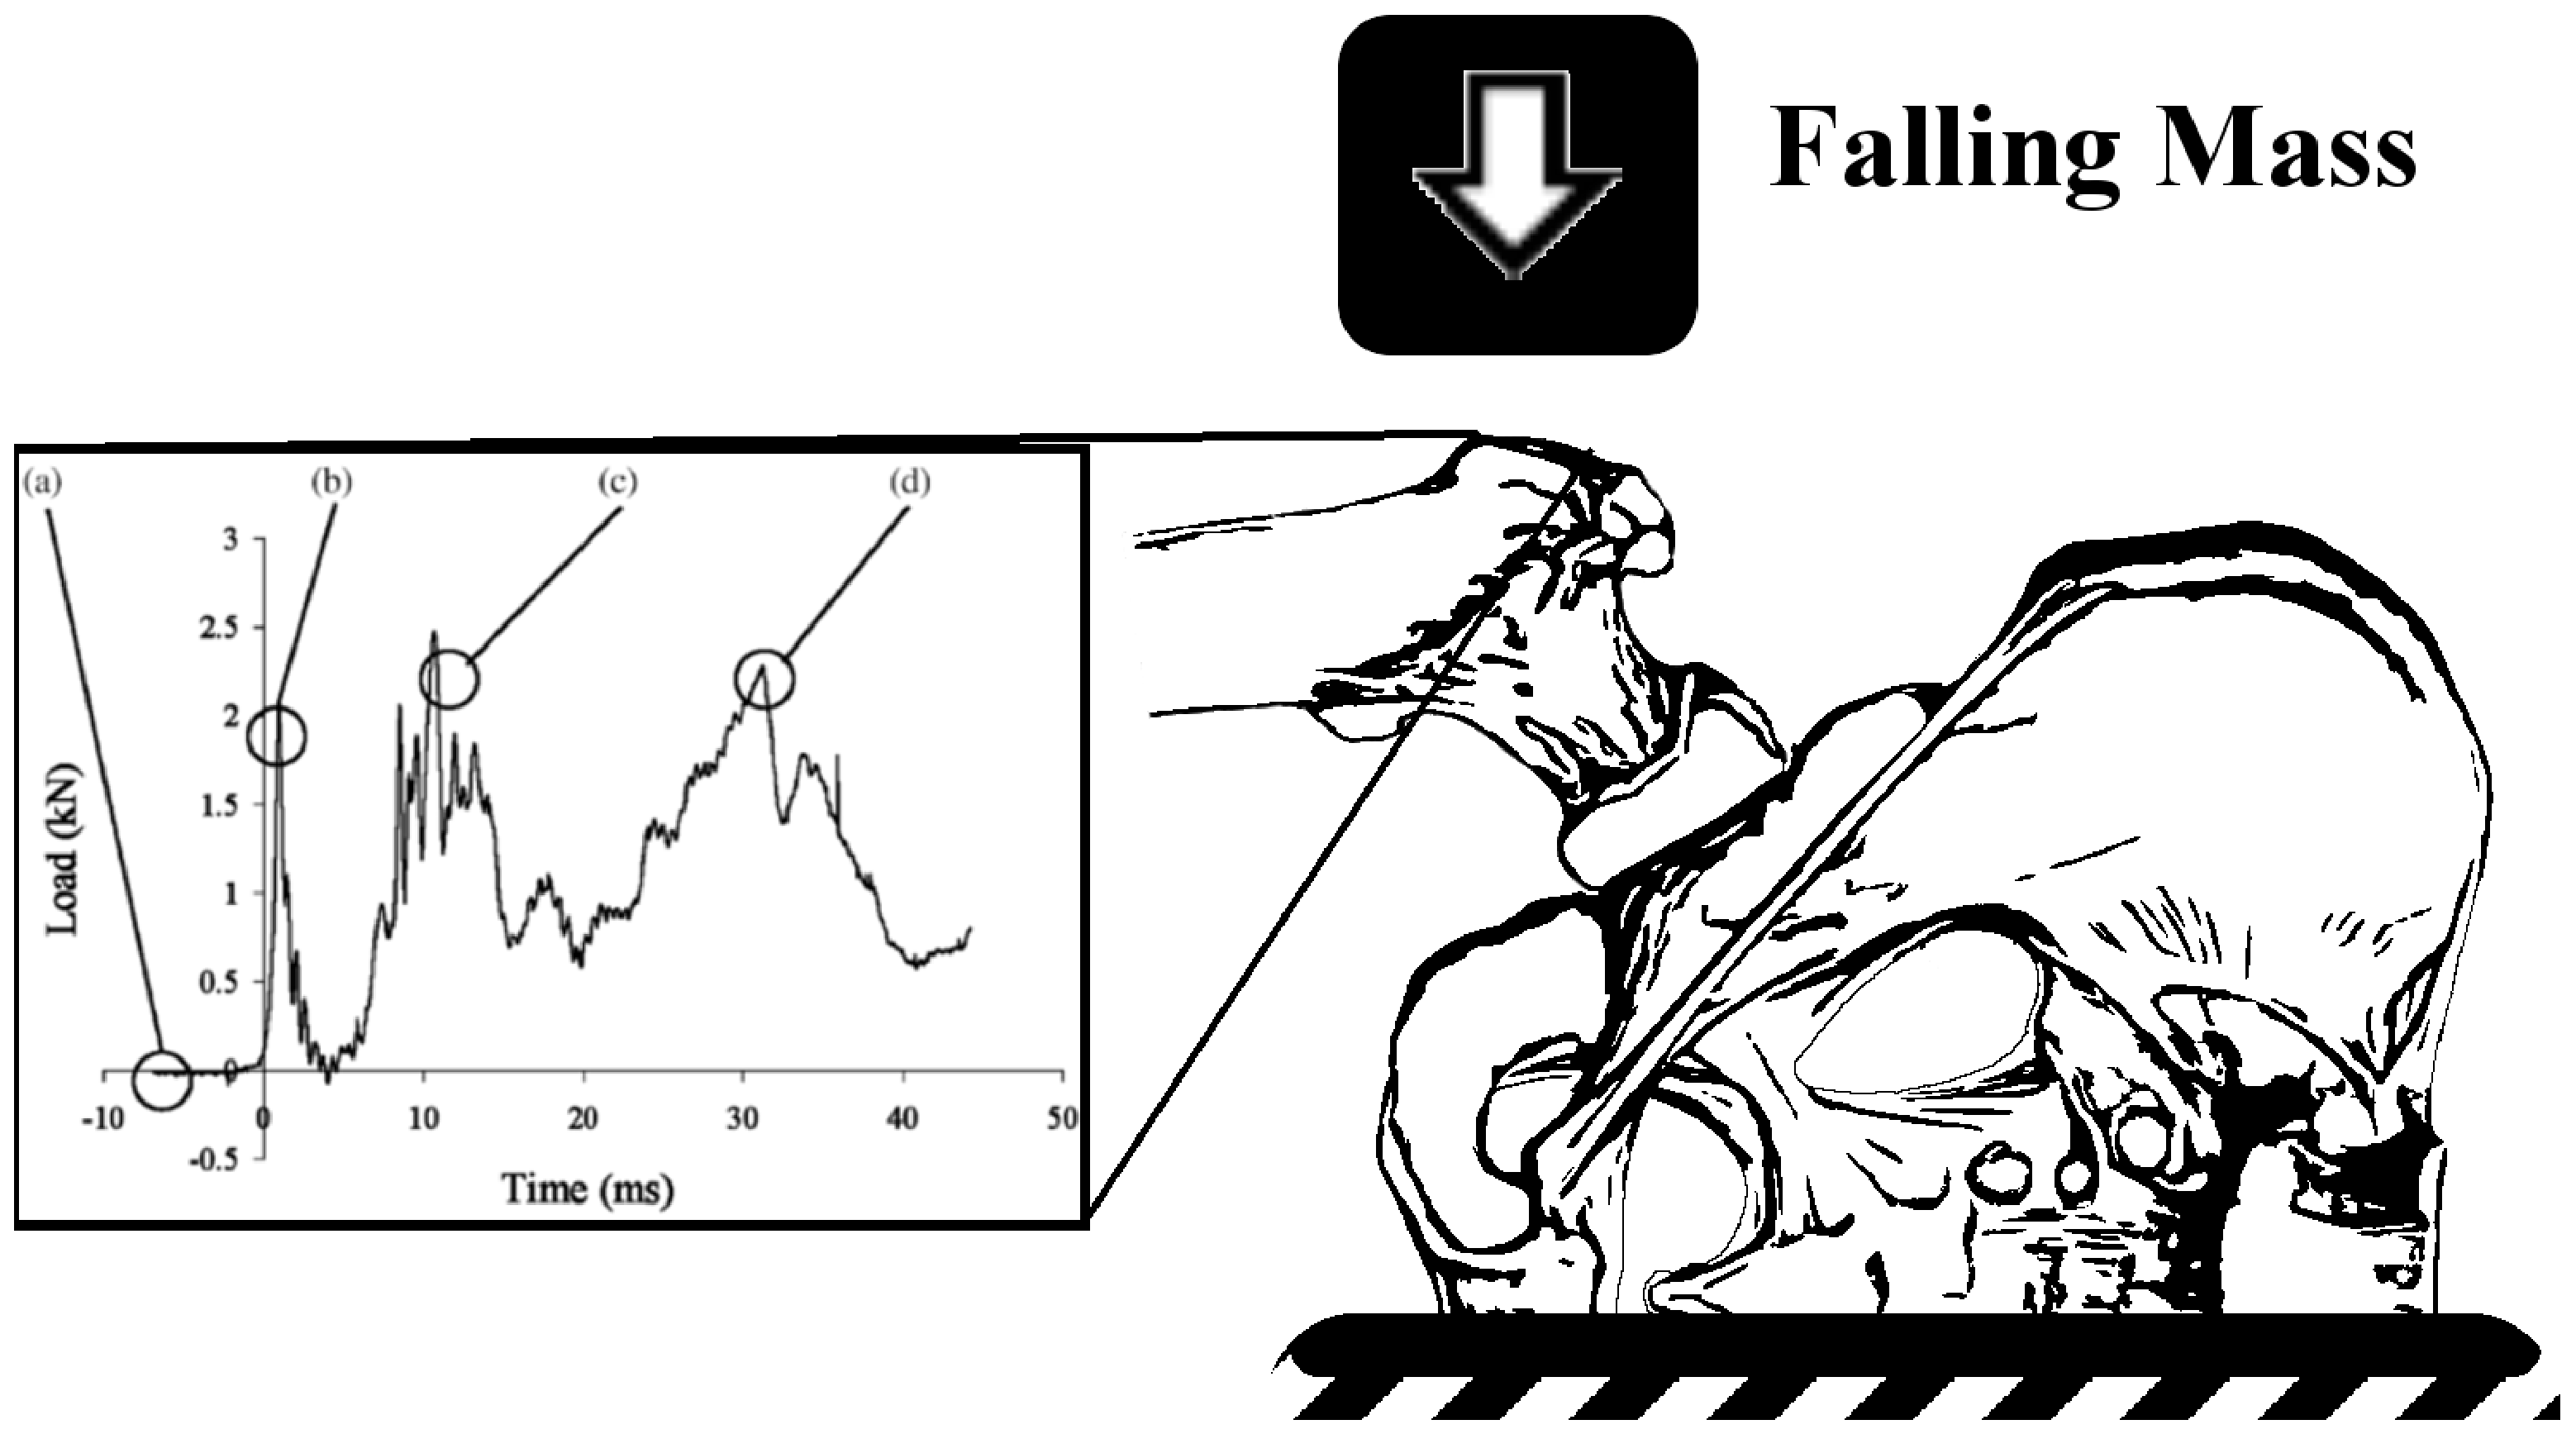
\includegraphics[width=1\linewidth]{./impactor/figures/BeasonComparison}
			\caption[Explanation of femur and lateral pelvis mass]{\textbf{In previous tests on osteoligamentous pelvises an instrumented impactor was dropped on the greater trochanter at 4.5~\ac{m}/\ac{s}.
			When the impactor came into contact with the trochanter a force spike was seen before deformation of the pelvis had begun, as indicated by peak (b) in the inset graph (adapted from \citet{beason_bone_2003}, with permission).
			This spike was created by the acceleration of the mass of the lateral pelvis and femur.}
			Illustrations adapted from \citet{gray_anatomy_1918}, copyright expired.}
			\label{fig:CompBeason}
		\end{figure}
		
		In the current apparatus, $m_{(eff\_p+f)}$ impacts a platen that is rigidly attached to a component used to hold and stabilize other parts of the apparatus (Figure \ref{fig:MassModel}).
		The mass of this stabilizing component influences the impulse delivered to the bone, and as such, the final value of $m_{(eff\_p+f)}$ needed to be tailored to the apparatus.
		The \textit{ex-vivo} value determined from the momentum analysis described above was used as a starting point for this process, and the mass was increased incrementally until the force delivered by the impulse matched a published, impact-velocity scaled, human volunteer test~\citep{laing_characterizing_2010}.
		The impact-velocity scaling was done by multiplying the human test by the ratio of (current experiment impact velocity)/(volunteer experiment impact velocity) which can be shown to be effective using impulse and vibration analysis.
		The final value for the pelvis mass was 1.98~\ac{kg}.

		\subsubsection{Pelvis stiffness}
		\label{sec:fall_sim_design_methods_apparatus_stiff}
		The pelvis has a finite stiffness, the value of which determines the duration of the impulse delivered by the effective body mass.
		This stiffness is not only a function of bone structure, but also body position at impact~\citep{robinovitch_distribution_1997, van_den_kroonenberg_hip_1996}, which must be taken into account when selecting the stiffness.
		Human volunteer experiments to characterize the stiffness of the pelvis~\citep{robinovitch_prediction_1991, robinovitch_distribution_1997, laing_characterizing_2010} have measured values ranging from 20.9 to 90~\ac{kn}/\ac{m}, depending on experimental protocol, and have shown its value to be constant above a compressive force of 300~\ac{n}~\citep{robinovitch_prediction_1991, laing_characterizing_2010}.
		Researchers used vibrational mechanics with various boundary conditions to determine the effective body mass and lateral stiffness of the pelvis~\citep{robinovitch_distribution_1997,laing_characterizing_2010} of human volunteers.
		The value of the effective body mass derived from one experimental condition~\citep{robinovitch_distribution_1997} was 32.8~\ac{kg}, which is similar to the effective body mass selected for the current experiment, and the corresponding pelvic stiffness was 35.4~$\pm$14.7~\ac{kn}/\ac{m}.
		This was selected as a base value for the current experiment, and was then modified to account for body position during the impact.
		
		Videos of volunteers falling have shown that people flex their trunks away from the ground at impact~\citep{van_den_kroonenberg_hip_1996, feldman_reducing_2007}, which increases the stiffness of the pelvis~\citep{robinovitch_distribution_1997}.
		To account for this, a spring with a rate of 50~\ac{kn}/\ac{m} was selected, corresponding to one standard deviation above the average stiffness for our base condition.
		The value of 50~\ac{kn}/\ac{m} also agreed with the recommendations of the international consensus statement for hip protector testing~\citep{robinovitch_hip_2009}.
		
		With the afore mentioned effective body mass and pelvis stiffness, the maximum anticipated deflection of the pelvis spring was 8~\ac{cm}.
		A steel spring with an outside diameter of 10~\ac{cm}, a free length of 35~\ac{cm}, and a maximum linear deflection of 18.6~\ac{cm} was used.
		A ratchet system with a tooth spacing of 9~\ac{mm} was incorporated to prevent rebound, as return of the stored energy post test was undesirable.

		\subsubsection{Soft tissue model}
		\label{sec:fall_sim_design_methods_apparatus_soft}
		Soft tissue over the greater trochanter is thought to protect the hip and prevent fractures in a sideways fall~\citep{majumder_effects_2008, robinovitch_prediction_1991, robinovitch_force_1995}.
		Researchers have shown that increasing the thickness of the soft tissue increases its ability to absorb and dissipate energy, thereby decreasing the potential for hip fracture.
		Computational work~\citep{majumder_effects_2008} showed a power-law relationship of $ Impact \; force \propto Thickness^{-0.2011}$.
		Experimental results from volunteer pelvis drop tests also showed a power-law trend of decreasing peak force with increased soft-tissue thickness, with a Spearman's $\rho$ = -0.71~\citep{robinovitch_prediction_1991}, and results from impact tests of cadaveric soft tissue~\citep{robinovitch_force_1995} showed that a 1~\ac{mm} increase in soft tissue thickness related linearly to a decrease in peak force of 70~\ac{n}.
		In the latter experiments, peak forces exceeded typical fracture forces for the proximal femur even for their highest tissue thickness of 45~\ac{mm}.
		
		Despite this understanding of how soft tissue attenuates impact force, epidemiological evidence of the protective nature of soft tissue is limited.
		Studies that have investigated the thickness of the soft tissue over the greater trochanter in fracture cases~\citep{bouxsein_contribution_2007, nielson_trochanteric_2009, minns_are_2007} have provided a pooled average and standard deviation of 29.4$\pm$15.6~\ac{mm}.
		Only a single study investigated the mechanical properties of the trochanteric soft tissue~\citep{laing_force_2008}, and showed that, while the stiffness of the tissue in the hip region of elderly individuals varied greatly with measurement location, they were typically around 20--35~\ac{kn}/\ac{m} over the greater trochanter when measured at a compressive stress of 100--140~kPa.
		
		For use in our fall simulator, a thickness one standard deviation below the average of fracture cases was selected in order to model an at-risk person.
		Due to material thickness availability, a final thickness of 19~\ac{mm} (0.75~inch) was chosen.
		This value also falls within the range recommended in the standardized hip protector testing protocol~\citep{robinovitch_hip_2009}.
		The material chosen had a stiffness of 26.5~\ac{kn}/\ac{m} at 95~kPa compressive stress (Evazote, Zotefoams Plc, Croydon, England), which was in the range of stiffnesses measured experimentally in the trochanteric region~\citep{laing_force_2008}.

		\subsubsection{Impact velocity}
		\label{sec:fall_sim_design_methods_apparatus_velocity}
		Impact velocity during a fall from standing is governed by two things.
		Firstly, the height of the person falling~\citep{van_den_kroonenberg_dynamic_1995}, and secondly any reactions, such as extending an arm to break the fall~\citep{feldman_reducing_2007}.
		Computational models~\citep{van_den_kroonenberg_dynamic_1995} of falls from standing have put the impact velocity at between 3.35 and 4.34~\ac{m}/\ac{s}.
		These values are higher than those observed in experimental tests where volunteers impacted their hips at a mean$\pm$SD of around 3$\pm$0.6~\ac{m}/\ac{s}~\citep{feldman_reducing_2007, van_den_kroonenberg_hip_1996}.
		
		An impact velocity of 3.0~\ac{m}/\ac{s} was selected based on the average of the volunteer tests~\citep{feldman_reducing_2007}.
		The specimen was placed stationary in the fall simulator (fall posture described below) and the effective body and pelvis+femur mass was dropped onto it.
		The effective body mass impacted the top of the pelvis spring, while $m_{(eff\_p+f)}$ bypassed the spring and contacted loading platens connected to the specimen through the soft-tissue model.
		To time these events so that they occurred coincidentally, $m_{(eff\_p+f)}$ was separated into two equal parts and suspended from the effective body mass by linear guide rods of length equal to the free length of the pelvis spring (Figures \ref{fig:MassModel} and \ref{fig:DT_setup}).
		This arrangement ensured that $m_{(eff\_p+f)}$ delivered a shock load at impact, and the effective body mass delivered a load mediated by the pelvis spring.

		\subsubsection{Specimen placement}
		\label{sec:fall_sim_design_methods_apparatus_placement}
		The surrogate bone was placed in the literature standard orientation for a fall to the side from standing.
		This orientation was, 10$^\circ$ adduction of the shaft and 15$^\circ$ internal rotation of the neck~\citep{courtney_effects_1994, de_bakker_during_2009, manske_cortical_2008, lochmuller_mechanical_2002}.
		Polymethylmethacrylate (PMMA, Bosworth Co, Skokie, IL) was used to make caps for the femoral head and lateral greater trochanter to prevent local crushing and also to provide even mounting surfaces.
		Each cap consisted of 20~\ac{g} of PMMA, formed by hand into a disk approximately 3.5~\ac{cm} in diameter, and moulded so that the head and trochanter loading surfaces were parallel.
	
	\subsection{Data collection and processing}
	\label{sec:fall_sim_design_methods_data}
	A six-axis load cell (Denton 4366J, Humanetics, Plymouth, MI), with an axial force capacity of $\pm$13.34~\ac{kn}, and non-linearity of $<$130~\ac{n}, recorded loads on the greater trochanter, between the pelvis spring and the specimen.
	
	Displacements of the greater trochanter and impact hammer were measured using a high speed video camera (Phantom v9, Vision Research, Wayne, NJ) imaging at 9216 frampes per second (fps) and a resolution of 576x288~\ac{px} (spatial resolution of 5~\ac{px}/\ac{mm}).
	Displacements were calculated from the video data using TEMA Automotive (v3.0, Image Systems, North Hollywood, CA).
	To determine the accuracy of this measurement, a validation study was carried out in which a bone surrogate (model 1130-21, Sawbones, Vashon, WA) was moved in a cyclic manner in the field of view of the displacement measurement camera.
	A dial gauge was recorded showing the displacement of the surrogate at any given time, and the results of the TEMA calculations were compared to the dial gauge at randomly selected times.
	The uncertainty of this measurement was determined to be $\pm$0.043~\ac{mm} ($\pm$\ac{sd}).
	
	Forces were recorded using a PCI-6040E (National Instruments, Austin, TX), 12~bit data acquisition board, and custom LabView software at a sampling rate of 20~\ac{khz}, with hardware anti-aliasing filtering at 10~\ac{khz}.
	The load cell outputs were amplified such that voltage saturation was attained at $\pm$6~\ac{kn}, giving a force resolution of 3~\ac{n}/bit.
	Imaging data was synchronized by recording a camera trigger signal generated by the drop tower gantry closing a switch as it fell.
	
	All data were forward and reverse, low-pass filtered using MatLab (2010b, The Mathworks, Natick, MA) with a -3~dB cut off at 500~\ac{hz}.
	Force data were processed with a fourth-order Butterworth filter and displacement data were processed with a second-order Butterworth filter.
	The cut off frequency of 500~\ac{hz} was chosen to remove high frequency ringing of the drop tower while retaining important impact events.
	The final fall simulator arrangement is shown in Figure \ref{fig:DT_setup}.
	
	\begin{figure}
		\centering
		\includegraphics[width=1.0\linewidth]{./impactor/figures/DT_setup2.eps}
		\caption[Photo of the fall simulator]{\textbf{A photo of the fall simulator showing each element of the model}}
		\label{fig:DT_setup}
	\end{figure}

	\subsection{Digital image correlation verification}
	\label{sec:fall_sim_design_methods_dic}
	A separate experiment was carried out to validate the use of \ac{dic} on the bone of the proximal femur for surface strain measurement.
	Subsequent tests in the fall simulator will use \ac{dic} strain measurement exclusively.
	
	Twenty human femoral specimens (3 normal, 11 osteopenic, 6 osteoporotic) were cleaned of soft tissue and periosteum, and a strain rosette (FRA-2-11-3LT, Tokyo Sokki Kenkyujo Co., Tokyo, Japan) was glued on the anterior-superior femoral neck using cyanoacrylate and a standard protocol~\citep[Chapter:~Strain gauge analysis of hard tissues: factors influencing measurements]{little_experimental_1992}.
	The femoral neck, including the strain gauge, of each specimen was painted with a white-on-black speckle pattern using an airbrush (VL, Paasche, Chicago, IL).
	The specimens were placed in a materials testing machine (8874, Instron, Norwood, MA) in the fall configuration~\citep{de_bakker_during_2009} discussed in \S\ref{sec:fall_sim_design_methods_apparatus_placement} and loaded to 50\% of their total aBMD predicted fracture load~\citep{boehm_prediction_2008}, at a constant compression rate of 0.5~\ac{mm}/\ac{s}.
	
	Force was output by the materials testing machine using a voltage scaling to provide 4~V at the target maximum load.
	Displacement was output with a constant scaling of 0.35~\ac{mm}/V.
	Three channels of strain data were collected at 20~\ac{khz} from the the strain rosettes using an SCXI-1520 strain gauge input module (National Instruments, Austin, TX) connected to the PCI-6040E, with hardware anti-alias filtering at 10~\ac{hz}.
	Two high speed video cameras (Phantom v12.1), recording at 100~fps and a resolution of 1280x800~\ac{px} (spatial resolution of approximately 17~\ac{px}/\ac{mm}), were used to observe the anterior-superior femoral neck including the strain gauge.	
	The video and voltage data were synchronized by recording the camera trigger signal which was emitted by the materials testing machine.
	The video images were imported into commercially available \ac{dic} software (StrainMaster, LaVison, G\"{o}ttingen Germany) for analysis.
	The \ac{dic} data were analysed using an iterative approach in which erroneous displacement vectors were identified as those that were \textgreater1.5~\ac{sd} from their immediate neighbours.
	These vectors were replaced by an average of their neighbours and reanalysed.
	After this second round of analysis, the strain field was filtered using a 3x3 median filter.
	The strain gauge data were taken as a gold standard measurement and the \ac{dic} data were compared to them in order to determine the \ac{dic}'s accuracy and precision.
	Comparisons were made using minimum principal strain since it is known to correlate to compressive failure~\citep{bayraktar_comparison_2004}.

\section{Results}
\label{sec:fall_sim_design_results}
The force-time profile of the fall simulator was compared to the same velocity-scaled human volunteer data discussed in \S\ref{sec:fall_sim_design_methods_apparatus_pelvis}.
The fall simulator and velocity-scaled human volunteer profiles were seen to be similar in timing and magnitude (Figure \ref{fig:CompareToLaing}).
The initial force peak in the fall simulator was 40\% higher than in the volunteer data and delayed by 5.2~\ac{ms}.
The average loading rate up to the initial peak was the same in both data sets, with a value of 122.4~\ac{kn}/\ac{s} in the fall simulator and 121.7~\ac{kn}/\ac{s} in the scaled volunteer data.
The force of the initial peak was observed to be increased by internal vibration of the pelvis spring, which can be seen as a sinusoidal variation throughout loading.
A Fourier analysis of the impact event showed that the amplitude of spring component was approximately 13\% of the dominant frequency component, however, its timing created a discrepancy in force equal to 80\% of the volunteer data at 16~\ac{ms} post impact.
The global peak force in the fall simulator was within 5~\ac{ms} of the volunteer data.
The rapid decrease in the fall simulator force after 50~\ac{ms} was due to the engagement of the ratchet, preventing rebound of the spring.

\begin{figure}
	\centering
	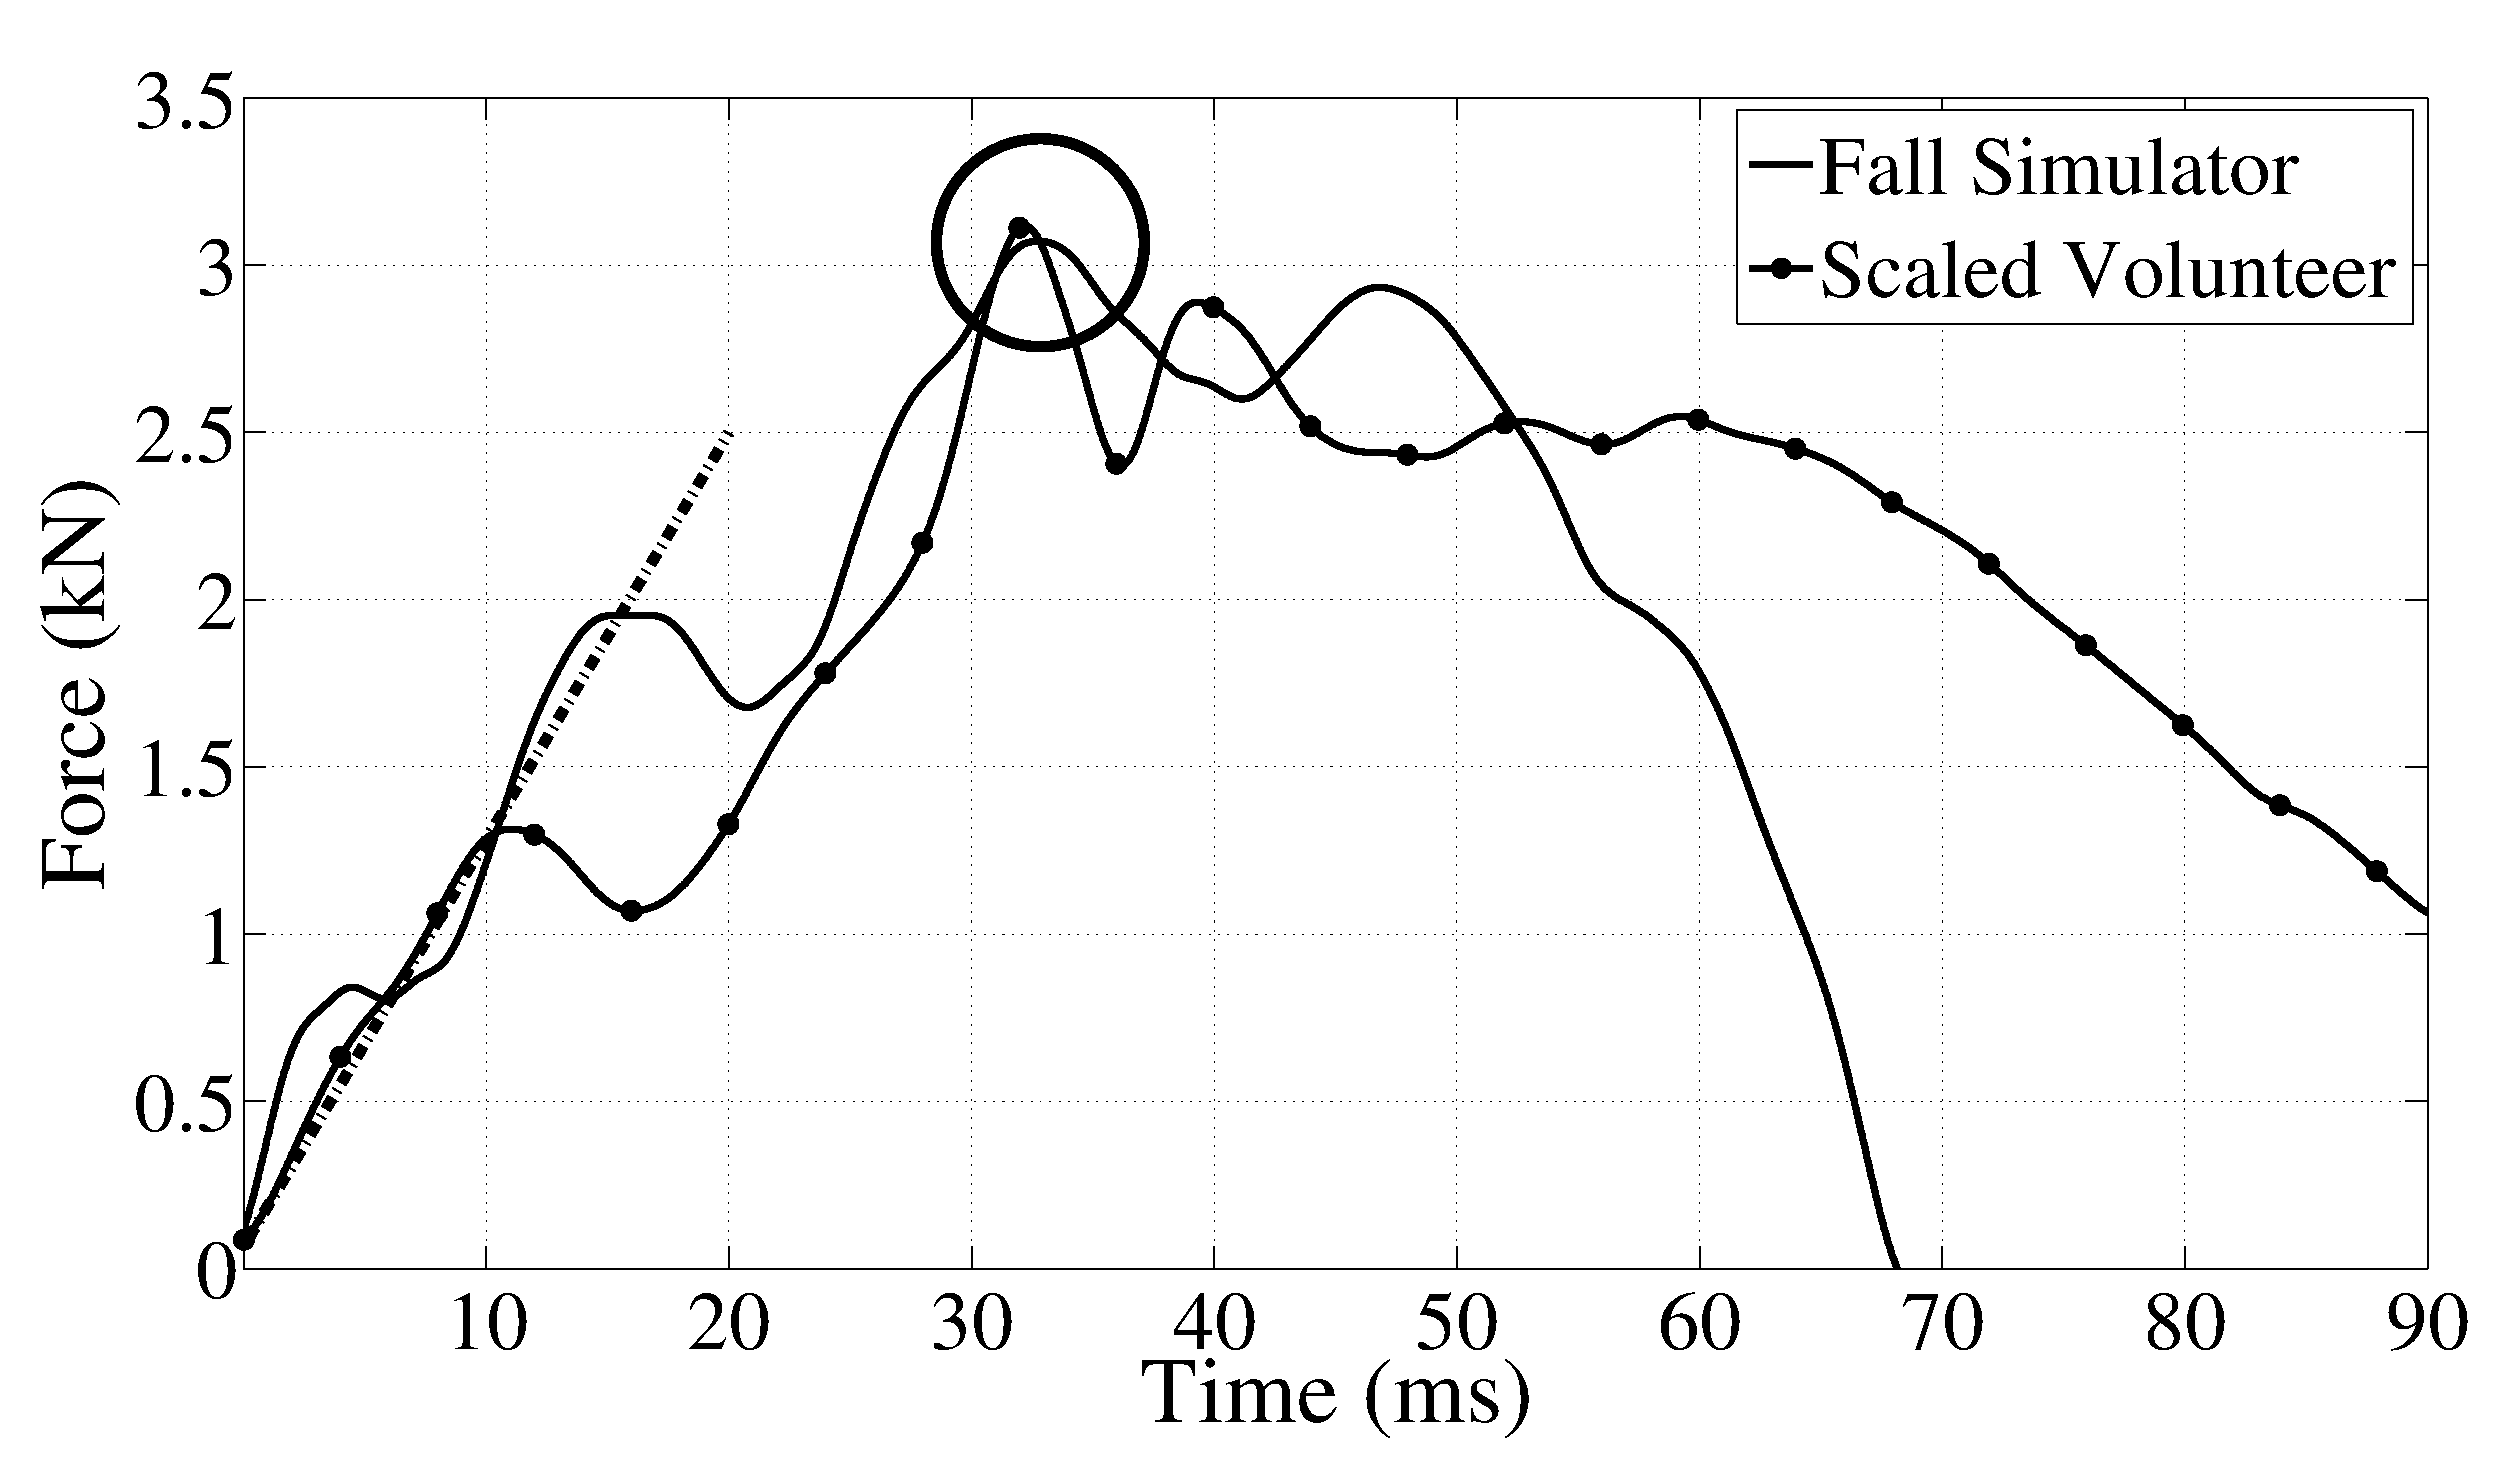
\includegraphics[width=1\linewidth]{./impactor/figures/CompareToLaing2010_VelocityScaled.eps}
	\caption[Fall simulator data compared to a human volunteer]{\textbf{An example response of the fall simulator plotted with human pelvis drop data~\citep{laing_characterizing_2010}.
	The dashed line indicates the initial loading slope of the scaled volunteer data and the circle indicates the location of the peak forces.
	The human data was scaled by the ratio of the impact velocities.}}
	\label{fig:CompareToLaing}
\end{figure}

In the \ac{dic} verification experiment, minimum principal strains from the \ac{dic} and the strain rosettes were well correlated (Figure \ref{fig:StrainErrors}).
The \ac{dic} result contained image-to-image noise (Figure \ref{fig:ExampleStrain}), the amplitude of this noise was found to be normally distributed and the frequency spectrum had no peaks in the range of 0-50~\ac{hz} (the Nyquist frequency), indicating that it was likely random in nature.
Three data sets (5, 8 and 10 in Figure \ref{fig:StrainErrors}) were subjected to camera vibration.
It is thought that one of the tripod legs was contacting the table supporting the materials testing machine, transferring vibrations associated with the hydraulic pump to the camera.
Identification of the faulty data sets was trivial, as strain would change by more than 1000~\ac{micro-eps} from frame to frame.
Excluding the datasets thus affected, the \ac{rms} average difference was 127~\ac{micro-eps} (range: [-375, 336]), and the standard deviation was 239~\ac{micro-eps}.

\begin{figure}
	\centering
	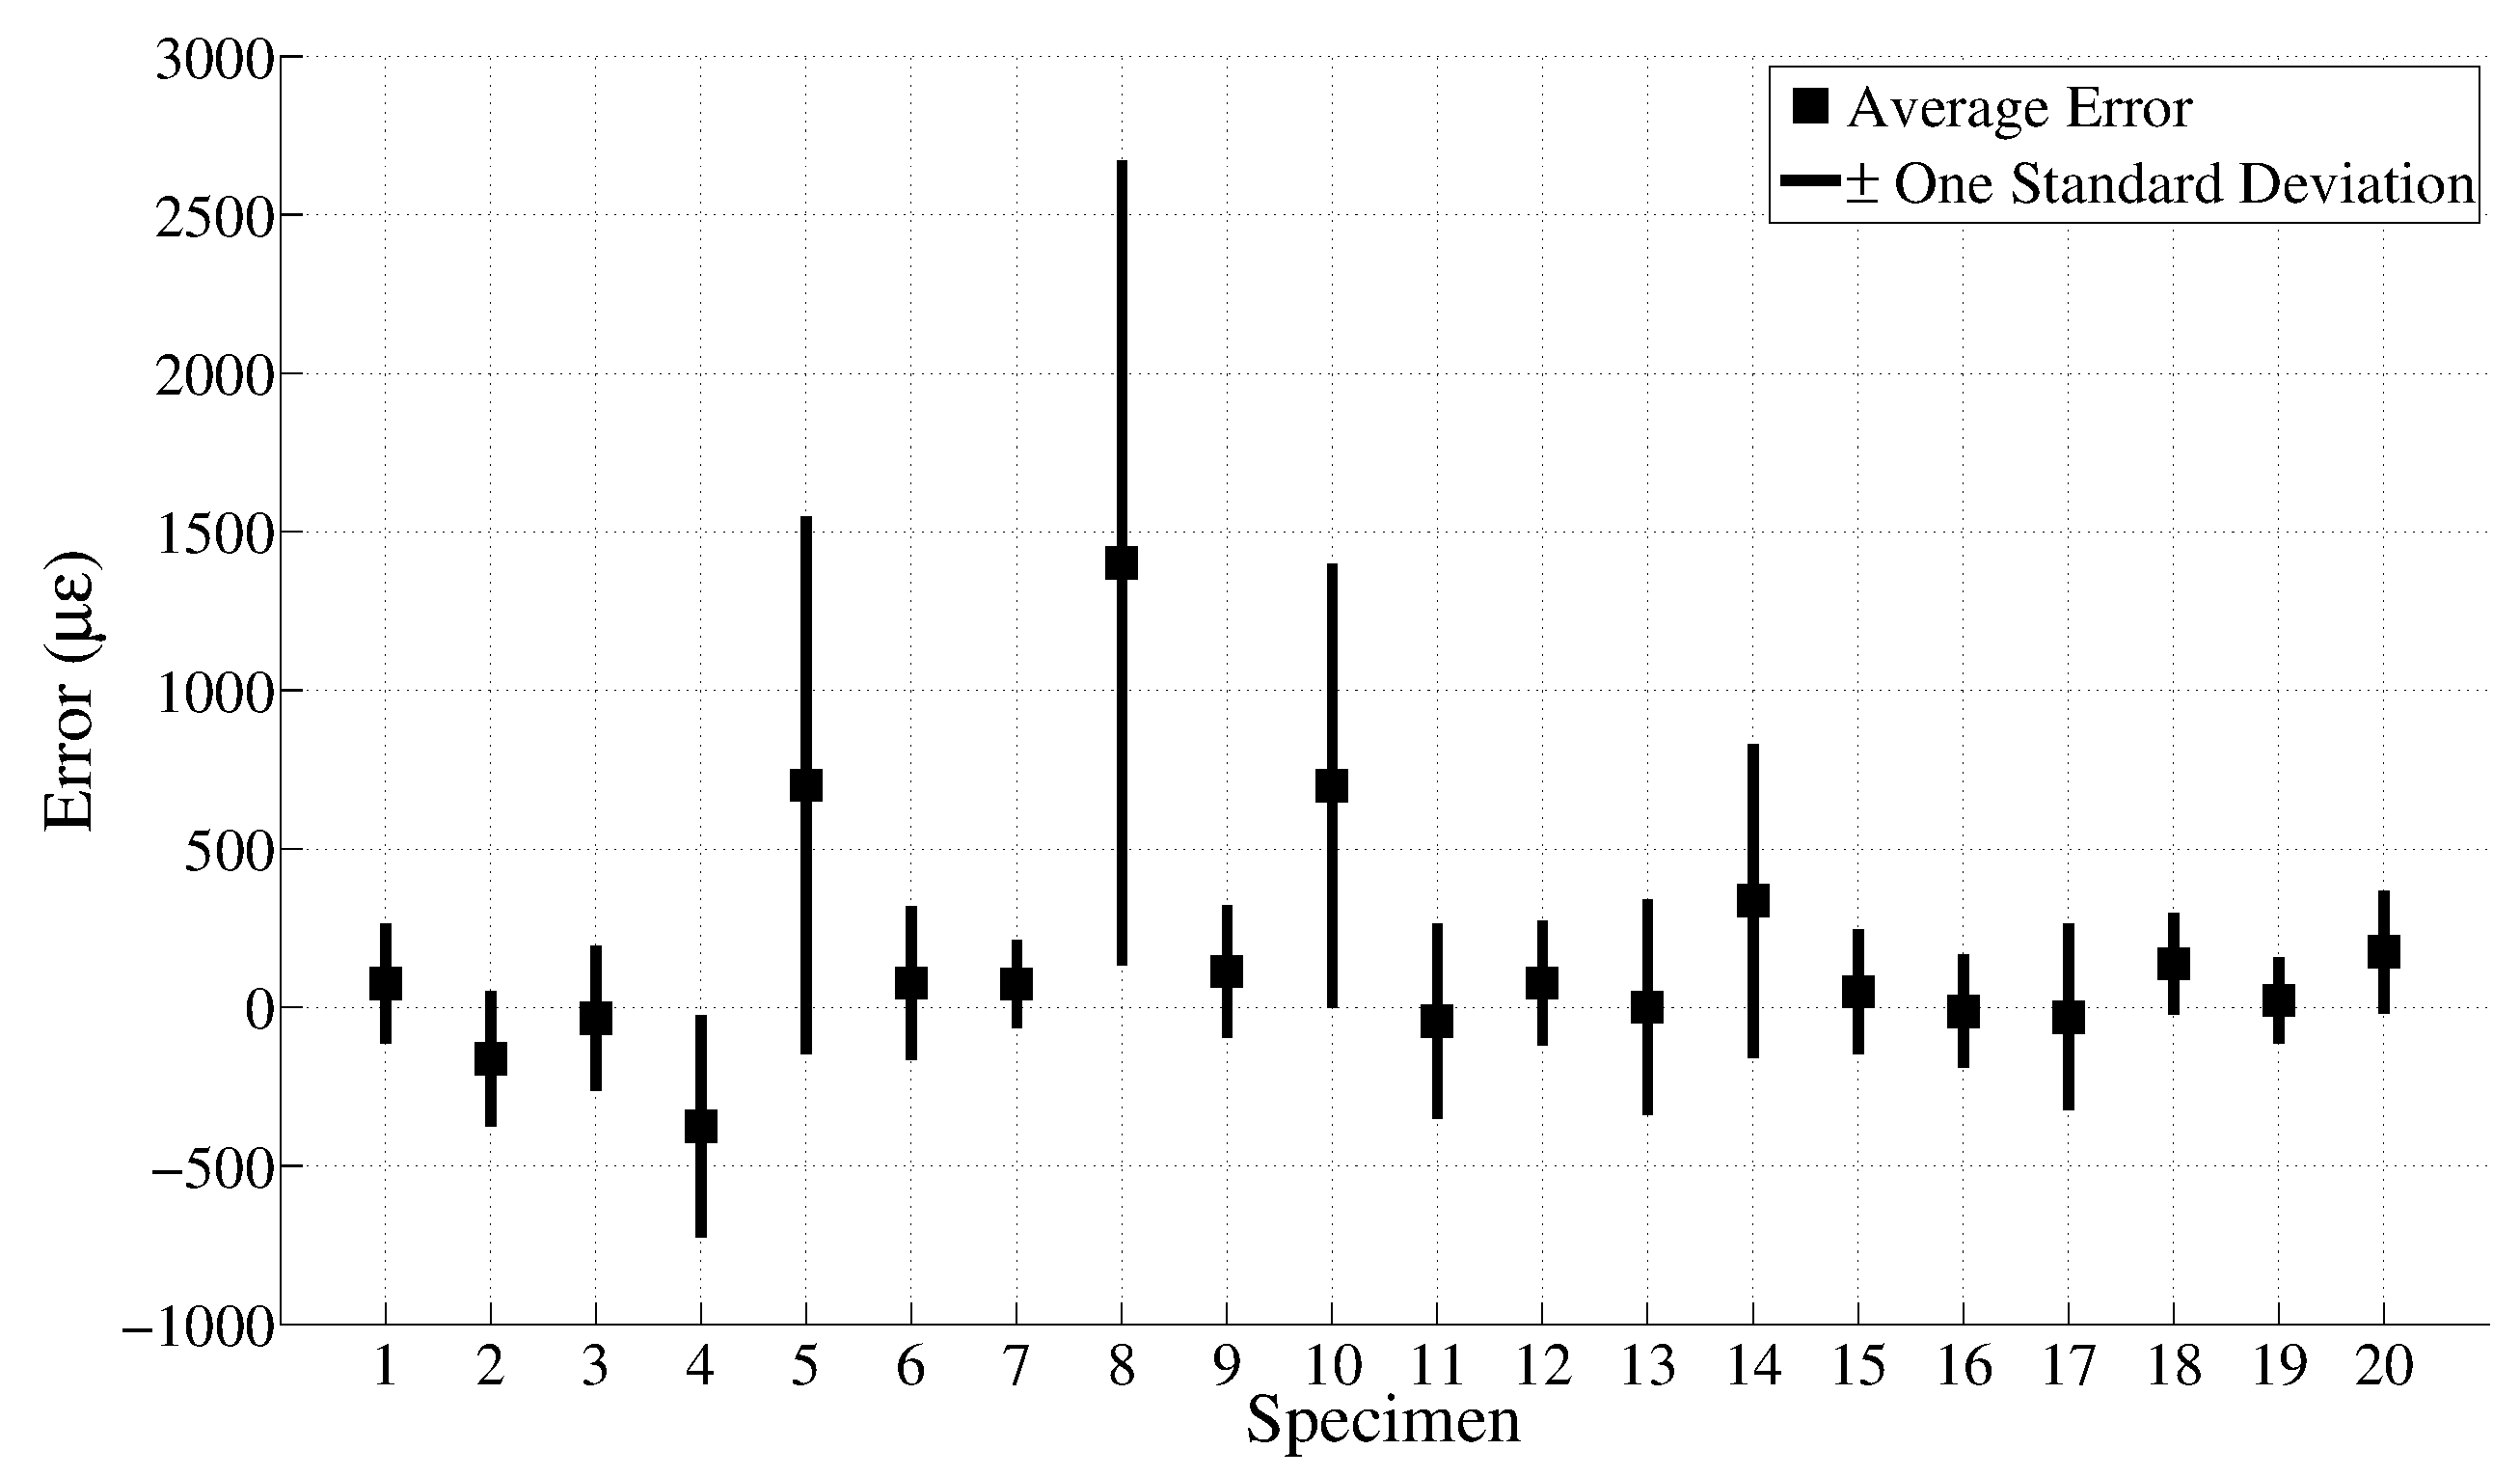
\includegraphics[width=1\linewidth]{./impactor/figures/StrainError.eps}
	\caption[Validation of \acf*{dic} on the femoral neck]{\textbf{The average and standard deviation of the strain errors measured for each specimen.
	Three specimens, 5, 8, and 10, were subjected to camera vibration, leading to incorrect \ac{dic} strain readings.}}
	\label{fig:StrainErrors}
\end{figure}

\begin{figure}
	\centering
	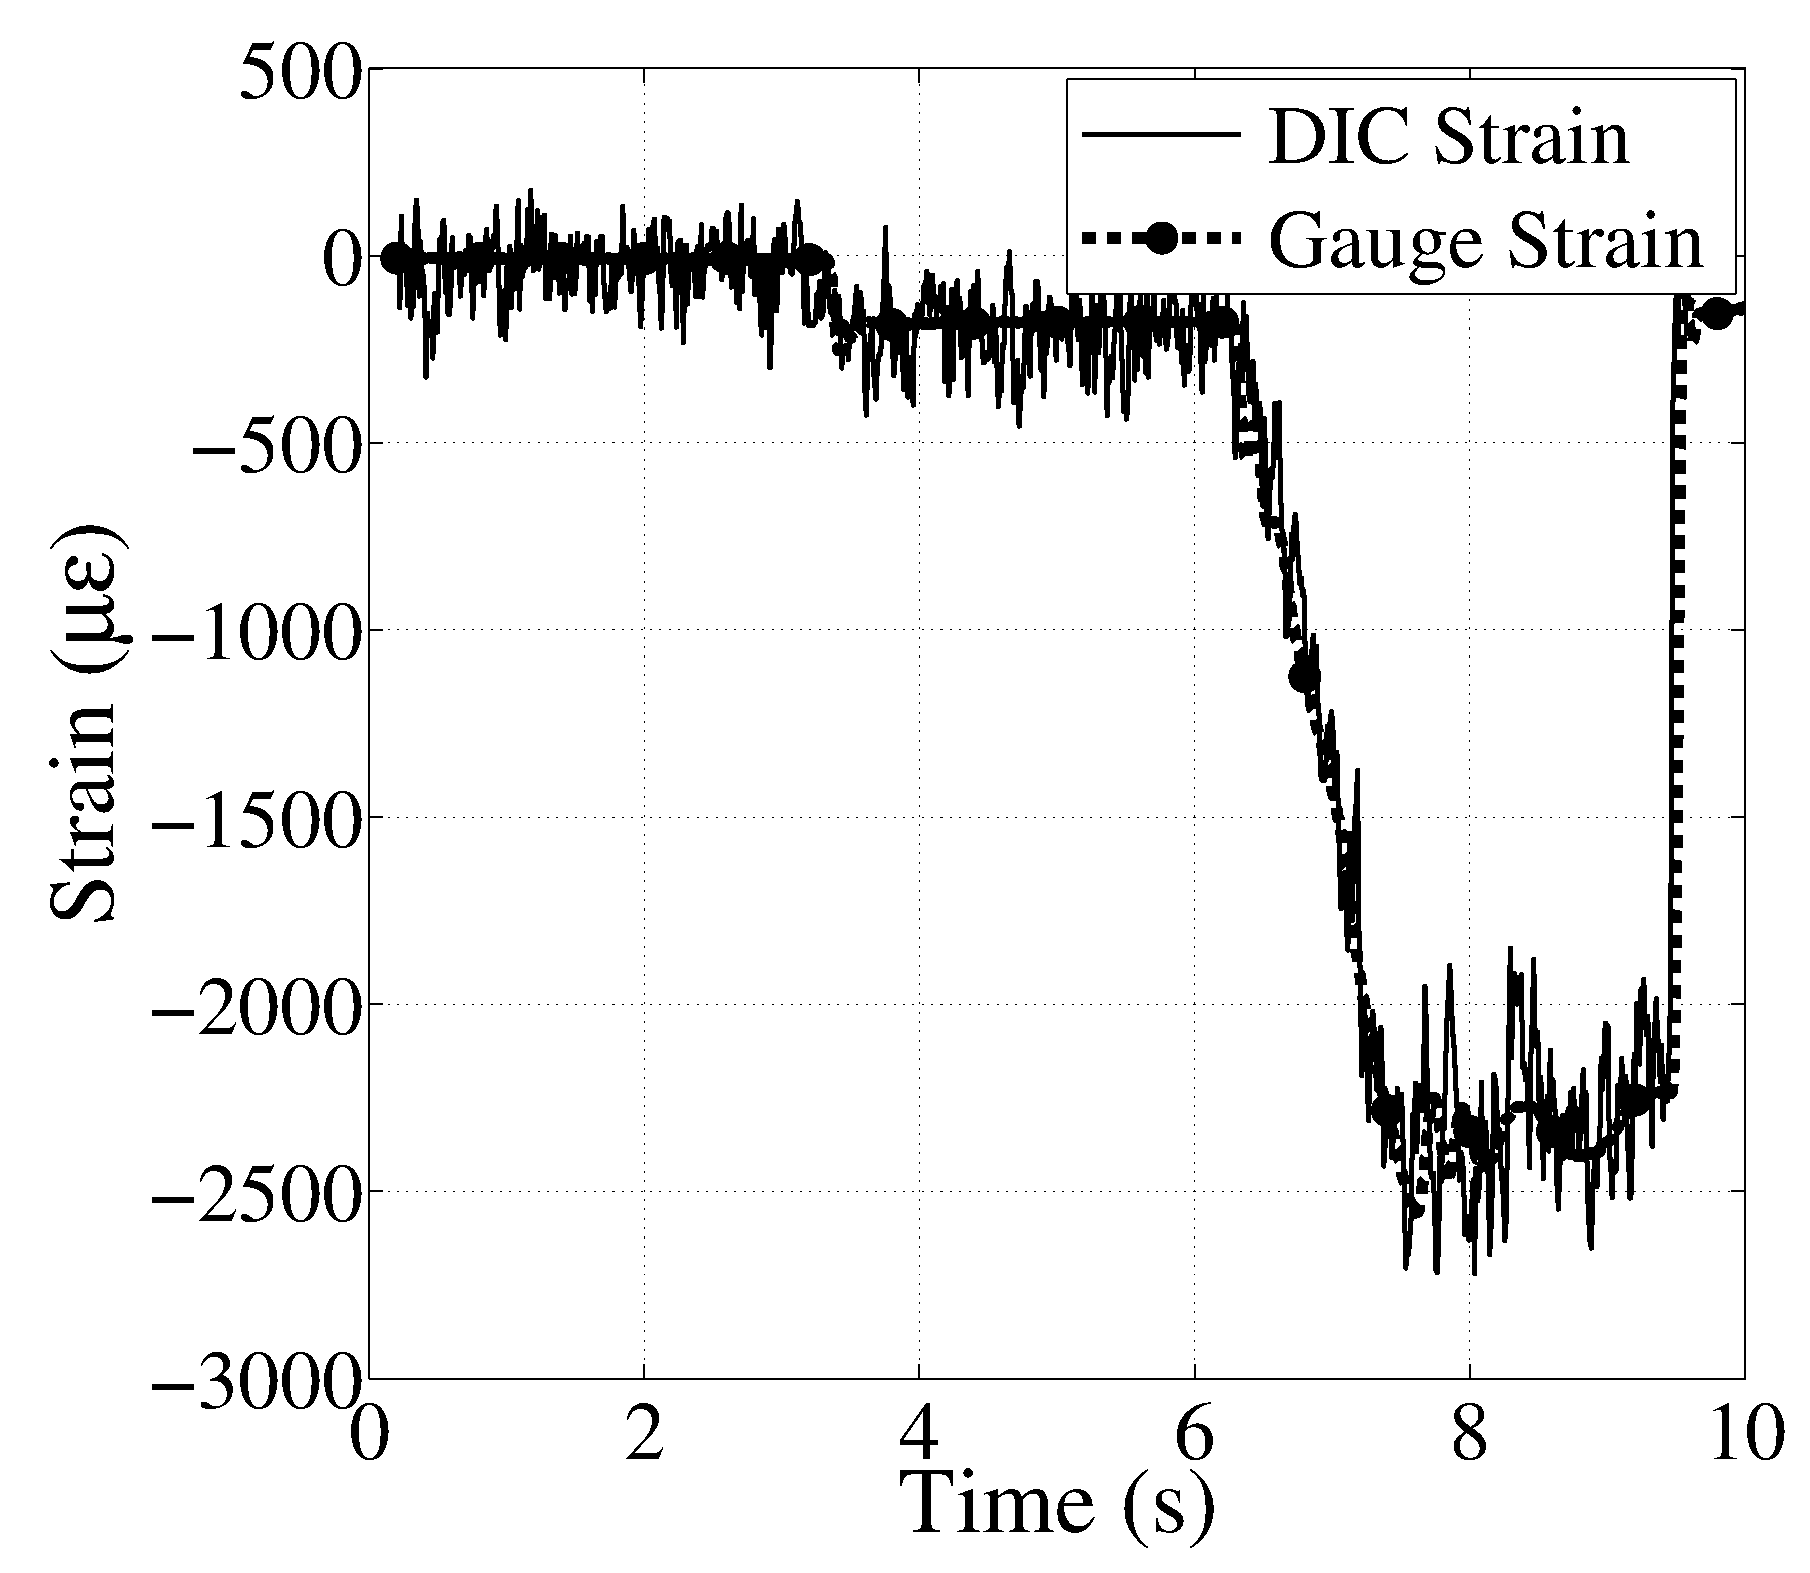
\includegraphics[width=0.7\linewidth]{./impactor/figures/StrainExample/StrainsTogether}
	\caption[Example \acs*{dic} strain and strain gauge data]{\textbf{Example data from the \ac{dic} analysis plotted with the strain gauge data. Time vs.\ strain plot for specimen 16 shows the character and magnitude of the random noise.}}
\end{figure}

\begin{figure}
	\centering
	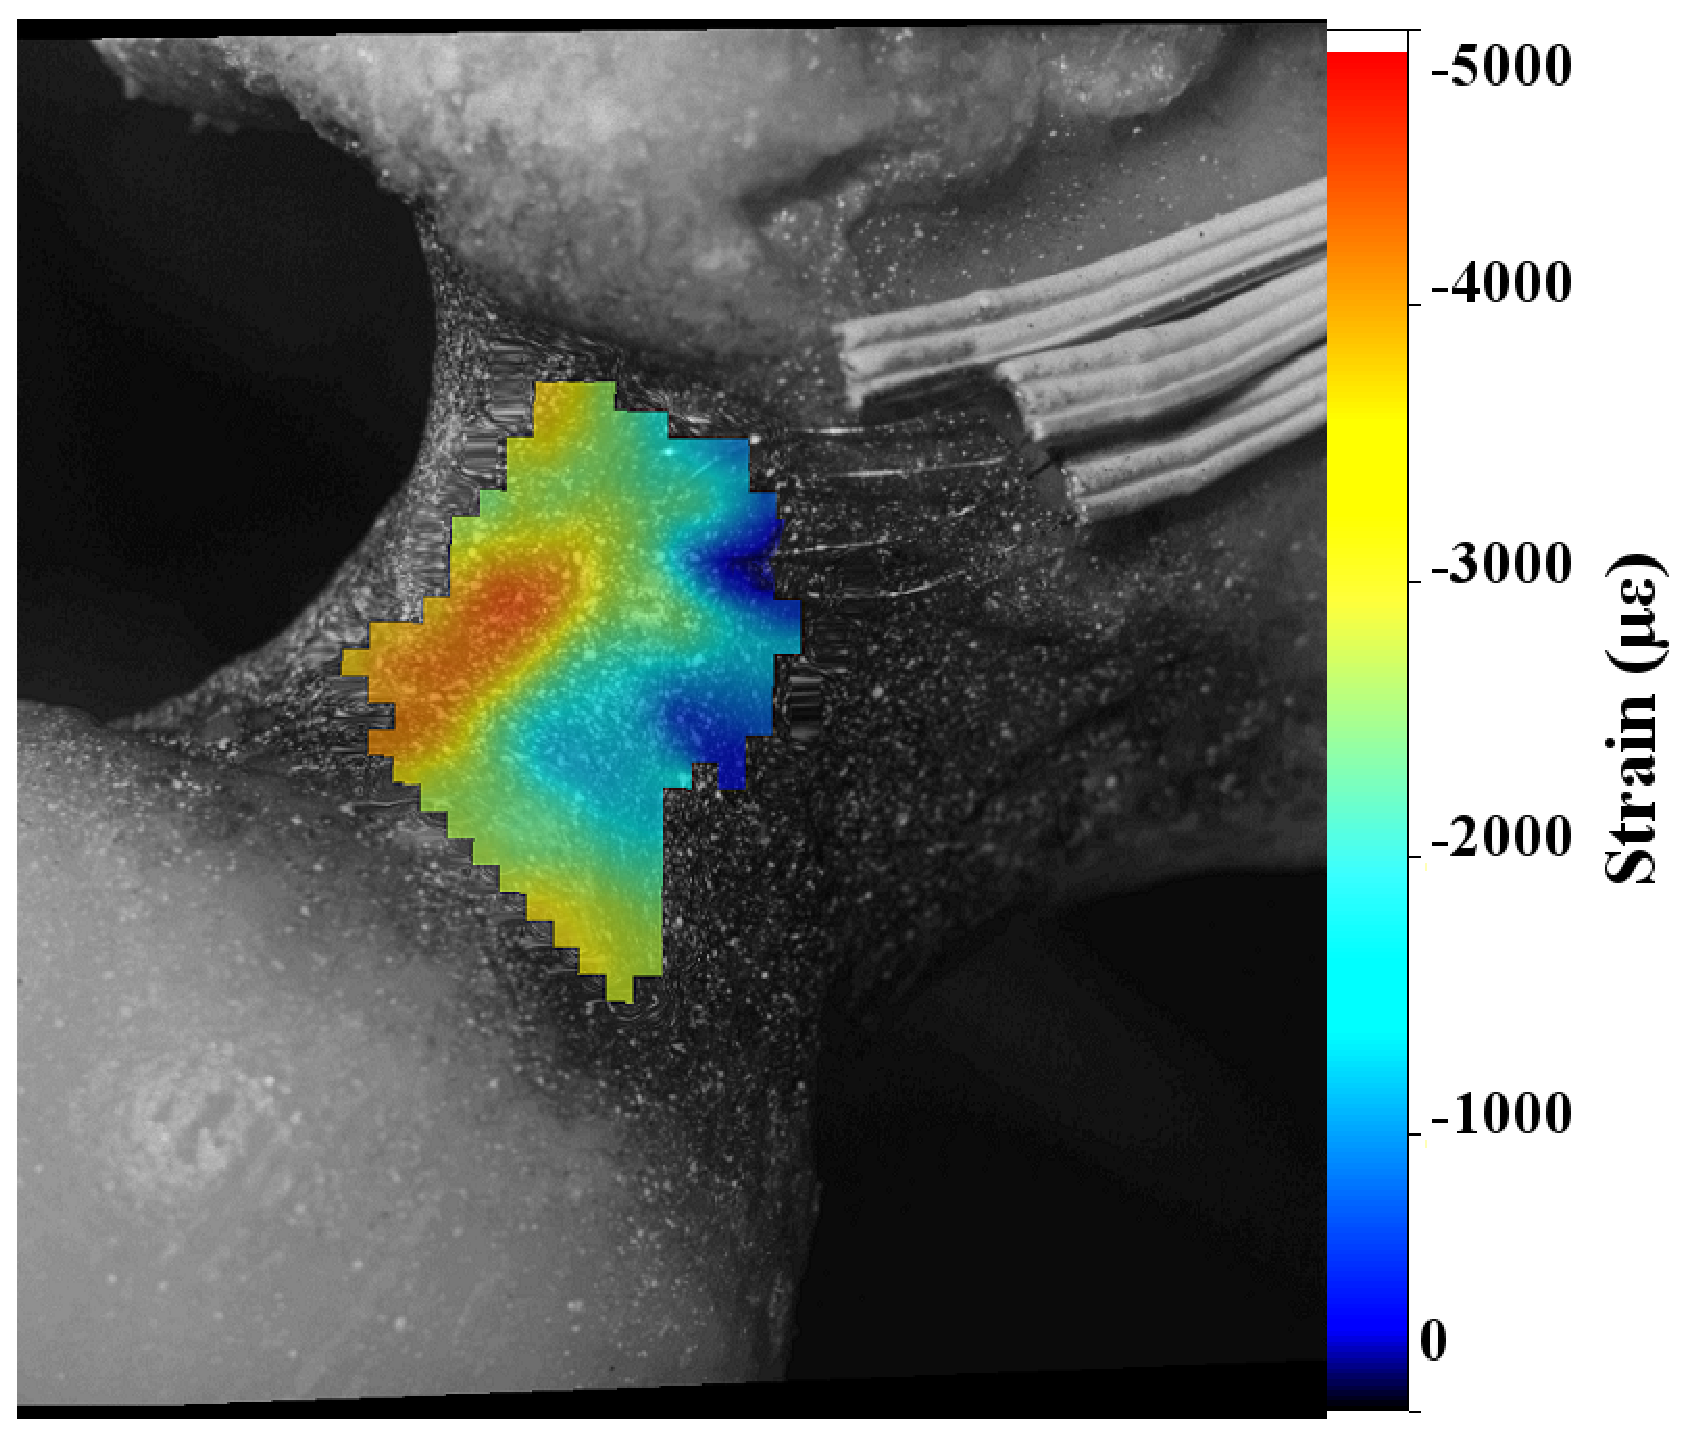
\includegraphics[width=0.7\linewidth]{./impactor/figures/StrainExample/H1376L_max_mod}
	\caption[Example surface strain data from the \acs*{dic} analysis]{\textbf{An example \ac{dic} strain contour map (b) shows how the strain varied over the surface of the bone at the maximum applied load. The bone is oriented such that superior is to the left and lateral to the top. The head of the femur is in the lower left and the trochanter occupies the upper portion of the image with the strain gauge wires visible on the right of the image.}}
	\label{fig:ExampleStrain}
\end{figure}

\section{Discussion}
\label{sec:fall_sim_design_discussion}
A method to simulate a fall to the side, impacting the greater trochanter of the femur, was developed.
A lumped parameter model of the human pelvis and hip joint, with the properties of each structure represented by literature values, was used.
Additionally, a method for full field strain analysis was validated on the neck of the proximal femur.

Previous researchers have developed models of the pelvis and body for use in hip protector testing~\citep{robinovitch_prediction_1991, robinovitch_hip_2009, laing_force_2008}, but a model appropriate for testing of cadaveric tissue has not been implemented.
The selected body mass and pelvis stiffness were similar to those selected by the previous researchers, which was reflected in the time to peak force being similar between our apparatus and theirs.
\citeauthor{robinovitch_force_1995}~\citep{robinovitch_force_1995, robinovitch_hip_2009} reported a time to peak force for their apparatus between 30 and 45~\ac{ms} post contact; our apparatus had a peak force at 32~\ac{ms}, with a plateau until $\sim$50~\ac{ms} due to oscillations of the pelvis spring.
The use of the ratchet to prevent rebound does not have an analogue in the previous literature because research on hip protectors used metal or plastic femur surrogates, which were not at risk of fracture during the test.
This change represents an adaptation required for testing of human material to obtain physiological fractures.

Another adaptation for physiological testing was changing the pelvis spring from mobile to stationary.
\citet{robinovitch_hip_2009} proposed two methods for fall simulation to test hip protectors, one of which used a moving linear spring, dropped in a drop tower similar to the current apparatus.
Our experiments using such an arrangement, in which the pelvis spring is dropped on the specimen, during the development of the current fall simulator, showed that the inertia of the spring's free-end was large enough to fracture a proximal femur before compression of the spring even began.
While the impulse due to the spring's mass may not be important for hip protector testing, which aims to attenuate the global force peak, it is important when testing cadaveric specimens.

One principal difference between the current fall simulator and the previous models, was the inclusion of the effective mass of the lateral pelvis and proximal femur.
Previous models neglected this mass and used signal filtering to remove artefacts created by shock loading and oscillations of the pelvis spring~\citep{robinovitch_force_1995, robinovitch_hip_2009}.
As discussed in $\S$\ref{sec:fall_sim_design_methods_apparatus_pelvis}, the impulse delivered by the effective mass of the lateral pelvis and proximal femur is physiologic and should be modelled.
This impulse creates a situation in the initial milliseconds of the impact of a high loading rate, which may change the behaviour of a human bone specimen in ways that are difficult to predict~\citep{mcelhaney_dynamic_1966, crowninshield_response_1974, robertson_compressive_1978, courtney_effects_1994, pithioux_comparison_2004, hansen_effect_2008, zioupos_microcracking_2008}.
The model showed that the magnitude of this impulse is determined more by the soft tissue mechanics than the stiffness of the bone.
A linear mathematical model of the current apparatus showed that the sensitivity of the impulse to the selected mass was low, with a 25\% increase in the mass changing the impulse magnitude by 6\%.
We believe that inclusion of this high loading rate portion of the curve may be important to gain an understanding of how the failure of the proximal femur is initiated and how it progresses.

The soft-tissue model in the current apparatus is minimal compared to those used in hip protector testing, in which researchers typically model the entire lateral trunk~\citep{laing_force_2008}.
Modelling of the trunk is a requirement for accurate fitting of the hip protectors but removes the possibility of observation of the femoral deformation.
The current apparatus required access to the femoral neck and trochanter for video observation.
A fall from standing might allow some of the energy to be dissipated to the surrounding tissues, however, an impact on the greater trochanter in a low BMI individual would likely have little energy dissipation into the surrounding tissues due to the prominence of the bony landmark.
Our fall simulator is modelling, in effect, the scenario that hip protectors are meant to address.

The impact velocity selected for the fall simulator was the average velocity from previously publish fall volunteer experiments~\citep{feldman_reducing_2007}.
This value is lower than the value of 3.4~\ac{m}/\ac{s} recommended by the international consensus statement on hip protector testing~\citep{robinovitch_hip_2009}.
The principal goal of the tests preformed for hip protector testing is to model a fall that would almost certainly create a fracture and see if it could be prevented through use of a biomechanical device.
The goal of the current research was not to model a severe fall, but to model a physiological fall that may, or may not result in fracture.
As mentioned in the introduction, previous hip fracture research tested all bones to failure.
The fall simulator described in this paper has the potential to identify bones that do not fracture in a fall to the side from standing, allowing further investigation of what is protective or detrimental to bone strength.

The orientation of the bone in the apparatus was selected based on preceding literature.
This placement is set by shaft angle from the vertical (adduction angle) and rotation of the neck (internal neck rotation).
Previous researchers selected the orientation by reviewing fracture studies and selecting adduction and neck rotation angles that created clinical fracture types~\citep{lotz_use_1990, backman_proximal_1957}.
The adduction angle was later modified to a more physiologic angle after video of human fall volunteers became available~\citep{courtney_effects_1994}.
The neck rotation angle has remained the same as it is difficult to evaluate its value in volunteers.
\Citet{feldman_reducing_2007} measured the angle of the contact point with the ground, around the circumference of the hip, in human volunteers who fell from standing height (the \emph{hip proximity angle}).
They found this angle to be an average angle of 8$^\circ$ posterior from directly lateral.
Combination of this value with the average femoral anteversion in the human population of 9.73$^\circ$~\citep{toogood_proximal_2009} gives an impact angle of 17.7$^\circ$, which is close to the and current value of 15$^\circ$.

Data processing for the current fall simulator differs from that proposed in previous work on hip protector testing.
Hip protector testing has used low pass filtering to clean unwanted artefacts from the signal by cutting off the signal at either 100~\ac{hz}~\citep{robinovitch_force_1995} or 50~\ac{hz}~\citep{robinovitch_hip_2009}.
The dynamics of the impulse delivered to the lateral trochanter, which we propose are seen by the proximal femur, are filtered out using such low cut-off frequencies.
We selected a value that retains the impulse at the trochanter and also retains the oscillations of the pelvis spring.
The filter cut-off frequency of 500~\ac{hz} provided us with a meaningful, but clean force-time trace, showing dynamical events that we believe are important to biofidelic modelling of physiologic falls to the side from standing.

Strain fields were obtained using \ac{dic} and verified at one location, using a triaxial strain rosette.
\ac{dic} has been used to measure the surface stains on porcine mandibles~\citep{yasuyuki_relationship_2009}, mouse tibiae~\citep{sztefek_using_2010} and on the surface of a plastic surrogate femur model~\citep{dickinson_experimental_2011}.
The magnitudes of strains measured on the mouse tibiae were compared with strain gauge measurements in similar locations on different specimens, but were not directly compared.
Due to the inhomogeneity of strain on the surface of the mouse tibiae, this comparison method has limited utility as a validation.
In the case of the plastic femur surrogate, \ac{dic} calculated strains were compared to a finite element model and found to agree in shape and magnitude.
However, the strain field on the plastic model was more uniform and did not display the high strain gradients seen in both our tests and those conducted on the mouse tibiae.
Our validation expanded upon both of these techniques by using a strain gauge, at the same time and location as \ac{dic}, to evaluate accuracy and precision of the \ac{dic} measurement on a human bone specimen.
The noise level of 230~\ac{micro-eps} is only 2.0\% of low rate yield strain, and 5.9\% of high rate yield strain of cortical bone in compression~\citep{hansen_effect_2008}.
Strain fields calculated by \ac{dic} in our experiments exhibited steep strain gradients, potentially due to the inhomogeneity of the bone in the human specimens.
This is similar to the strain fields seen in previous research~\citep{sztefek_using_2010}, and justifies the utility of \ac{dic} over point strain measurements.

We have developed a method to simulate a fall to the side from standing that addressed several limitations of previous fall models.
Our goal was to increase the biofidelity of physiologic fall modelling and we have included many aspects of the anatomy and impact that were previously omitted.
In light of these advances, there are notable limitations to discuss.
Firstly, the pelvis stiffness model included a spring which had a large mass and exhibited its own vibrations, influencing the overall loading pattern.
A number of different avenues for elimination of this artefact were investigated, including rubber dampening, as well as composite and elastomer springs.
Each of these came with its own limitations of either increasing the mass of the spring further, being difficult to characterize or being highly non-linear.
The limitation of a non-ideal spring (\ac{ie}, a spring with mass) is nearly impossible to eliminate, however, it was mitigated through the use of the ratchet system and by starting the test with the spring stationary.
We believe that the advantages of the drop tower method, namely free response of the specimen and biofidelic loading, outweigh the limitation imposed by the spring.
Secondly, the pelvis model lacks a damping element, which in life is the consequence of the soft tissues surrounding the pelvis.
Previous literature examined the potential range of damping of the pelvis and found a average value of 520$\pm$340~\ac{n}\ac{s}/\ac{m}~\citep{robinovitch_distribution_1997}.
Using fundamental vibrational mechanics, and our chosen mass, spring and initial velocity, inclusion of this damping would change the peak force by between 0.3\% and 6.3\%, with an average change of 2.2\%.
We believe this variation is acceptable in the context of human variability.
Third, the soft tissue model used in the current fall simulator is limited by the need to visualize the bone throughout the impact, and does not allow for transfer of force and energy to tissues that, in life, would surround the proximal femur.
In effect, our apparatus simulates individuals that are slender and have prominent trochanters, which are a target population for hip fracture prevention~\citep{nguyen_identification_2005}.
We feel the limitation of only modelling a subset of individuals based on soft tissue thickness is outweighed by the benefit of fracture visualization.
Fourthly, the impact model developed includes only the effective mass of the body that is active in the lateral direction.
In a fall to the side there are other important masses and inertias at play, namely the \ac{s-i} constraint on the femoral head by the mass of the body, and the rotational, mass, and friction constraints on the distal leg.
The \ac{s-i} constraint on femoral head will likely affect the final fracture lines produced more than the mechanical and failure behaviours of the bone.
Relaxed constraint of the lower leg would allow the orientation of the bone to change throughout the impact and could lead to different mechanical behaviours.
The added biofidelity of the latter change could lead to highly complex dynamics that would be difficult to analyse and reproduce, decreasing the consistency of the experimental boundary conditions.
Finally, fixed parameters for each of the elements in the apparatus reduces the ability to model a subject-specific fall for each femoral specimen.
A subject-specific design, allowing variation of the body mass, soft tissue thickness, and possibly, pelvis stiffness and $m_{(eff\_p+f)}$ would increase the biofidelity of the model.
However, the current level of understanding of how the parameters would vary based on body morphology is limited, and making appropriate changes would be difficult.
Additionally, changing all the experimental parameters in this manner would reduce the statistical power of a given set of experiments and greatly increase the required number of specimens.
The current arrangement of a set apparatus, with the only variable between experiments being the specimen, provides a way to identify specimens of interest in a manner that is efficient and statistically powerful.

Our method, which is driven by the energy of a free falling mass representing a person falling from standing, removes artificial imposition of trochanteric displacement rate and allows each specimen to deform based on local response and failure, permitting visualization of a specimen's physiologic failure progression.
In future experiments, we plan to test a multitude of specimens using this apparatus, characterize the fracture progression and compare the free response behaviour to the behaviour seen in previous fixed displacement rate experiments.
We believe that understanding how the mechanics change under dynamic loading will allow us to better understand hip fracture, eventually leading to improved prevention, detection and treatment of this debilitating condition.


\acused{fs}
\acused{QS}
\acused{qs}
\acused{sim}
\acused{vs}
\acused{pt}
\acused{pw}
\acused{r2}
\chapter{Impact and constant displacement rate loading change the mechanical response of the femur in sideways fall simulation}
\label{ch:behave_fail}
To address the research questions outlined in \S\ref{sec:intro_method_behave} and \S\ref{sec:intro_method_fail}, specimens were loaded to sub-failure forces using quasi-static, constant displacement rate methods, and then loaded to failure in the fall simulator.
The behaviour in the sub-failure and failure loading were compared at the same force in terms of stiffness, energy, and point strain.
The specimens were then compared to two previously fractured specimen groups that were tested at 2~\ac{mm}/\ac{s}~\citep{nishiyama_proximal_2013} and 100~\ac{mm}/\ac{s}~\citep{de_bakker_during_2009} in terms of stiffness, energy to failure and maximum force.

The research presented in this chapter has been submitted for publication in the Journal of Biomechanics~\citep{gilchrist_mechanics_2013}.

\section{Introduction}
Hip fracture is a devastating injury associated with high mortality, morbidity, and high economic costs, on both personal and social levels \citep{braithwaite_estimating_2003, wiktorowicz_economic_2001}.
One of the critical avenues for reducing the burden of hip fracture has been early identification of potential hip fracture patients~\citep{johnell_predictive_2005, kanis_frax_2009, van_den_bergh_assessment_2010}.
Clinically, early identification is done using \acf{abmd} as measured by \acf{dxa}, but this technique has been shown to capture fewer than 30\% of those who suffer a hip fracture~\citep{stone_bmd_2003}.
One factor that may contributes to this discrepancy is a lack of understanding of the mechanism of hip fracture.
Increased understanding of the fracture mechanics of the proximal femur could aid the development of specific and sensitive tools for identifying people at risk of hip fracture.

Biomechanical researchers have utilized mechanical testing and computational modelling to study how the proximal femur fails in a fall to the side~\citep{keyak_prediction_1998, keyak_prediction_2000, verhulp_comparison_2006, verhulp_load_2008, srinivasan_relationship_2011, koivumaki_ct-based_2012}.
These researchers have identified the roles of bone density \citep{lotz_use_1990, courtney_age-related_1995, leichter_optical_2001, lochmuller_mechanical_2002, eckstein_reproducibility_2004, boehm_prediction_2008, manske_cortical_2008, de_bakker_during_2009, pulkkinen_experimental_2008}, posture \citep{pinilla_impact_1996}, displacement rate \citep{ weber_proximal_1992, courtney_effects_1994}, geometry \citep{cheng_assessment_1997}, and loading configuration \citep{keyak_prediction_1998, keyak_relationships_2000}.
While these data have contributed greatly to the current understanding of hip fracture, they were conducted using constant displacement rate protocols.
There may be differences in the mechanics of the proximal femur in an impact loading situation that would be important for understanding and interpreting the previous results.

In a fall to the side, the displacement rate~(\ac{mm}/\ac{s}) of the proximal femur is not prescribed or constant.
Instead, it is dictated by the dynamics of the fall and the response of the body under impact.
The femur acts as a compliant member in a spring-mass system which includes the body, the pelvis, and soft tissues surrounding the femur.
During the fall, the instantaneous value of a femur's compliance influences its displacement and loading rates~(\ac{n}/\ac{s}), which in turn alter the bone's mechanical behaviour in a rapid and complex way \citep{carter_compressive_1977, linde_mechanical_1991}.
We believe that the recursive nature of this relationship makes it essential to model the fall in order to measure, and visualize, the actual progression of failure of the proximal femur.
Because the femur has not been studied under these conditions previously, it is not known if the behaviour or mechanics of the femur are different between the historical laboratory simulations and real-world falls to the side.

The objectives of this research were to determine if: i) femoral deformation in constant displacement rate and impact testing are different; ii) femoral failure characteristics are different between the two loading methods; and iii) to characterize the free-response force and displacement curves in a biofidelic impact.
We hypothesized that the proximal femur's sub-failure force-displacement and strain behaviours would be different between low displacement rate loading, and inertia-driven fall simulation.
Further, we hypothesized that the proximal femurs' failure mechanics would be different between fixed displacement rate and fall simulation failure tests. 
We also characterized the loading and displacement rates in the fall simulation tests, and examined their relationships with specimen stiffness.

\section{Materials and methods}
Three groups of specimens were used in this analysis.
These were the specimen groups used by \citet{de_bakker_during_2009} and \citet{nishiyama_proximal_2013}, tested in our lab under constant displacement rates, and an additional 21 specimens that were tested in the combined high sub-failure + inertial fall simulation protocol (Table~\ref{tab:summary}).
The specimens will be referenced by how displacement was applied to each; those from \citet{nishiyama_proximal_2013} will be referred to as the \textit{slow} group; those from \citet{de_bakker_during_2009} will be referred to as the \textit{fast} group; and the specimens in the current test will be referred to as the \textit{fall} group because they were failed using the fall simulator.
Each specimen in the fall group was subjected to two test conditions, a quasi-static, constant displacement rate, sub-failure test (fall:\ac{QS}) and an inertially-driven, fall simulation failure test (fall:\ac{fs}).

\begin{table}
\centering
\begin{threeparttable}
\caption[Specimen groups]{Specimen groups showing identifying characteristics. The slow~\citep{nishiyama_proximal_2013} and fast~\citep{de_bakker_during_2009} groups are discussed in more detail in previous publications. The specimens in Fall:\ac{QS} and Fall:\ac{fs} are from the same specimen group, but include different specimens based on data availability. Comparisons between these two groups were restricted to specimens tested using both methods. Numbers are shown as mean~(standard deviation).}
\label{tab:specimens}
\begin{tabularx}{\textwidth}{>{\centering\arraybackslash}X >{\centering\arraybackslash}X >{\centering\arraybackslash}X >{\centering\arraybackslash}X >{\centering\arraybackslash}X >{\centering\arraybackslash}X}
\toprule
\multirow{2}{*}{Group}	&
\lbCell{Age \\ (Years)}	&
\lbCell{Number and \\ Gender}  &
\lbCell{\acs{abmd} \\ (\acs{g}/\acs{cm}$^2$)}	&
\lbCell{Displacement \\ Rate (\acs{mm}/\acs{s})}	&
\lbCell{Loading \\ Rate (\acs{kn}/\acs{s})} \\ \midrule
Slow		& 77 (13) & 4M, 14F & 0.613 (0.164)	& 2 				& 0.5 (0.16)\tnote{*} \\
Fast		& 84 (7)  & 6M, 5F  & 0.763 (0.150)	& 100				& 33 (8)\tnote{*} \\
Fall:\acs{QS}		& 77 (10) & 1M, 19F	& 0.707 (0.108) & 0.5 				& 0.22 (0.16)\tnote{*}\\
Fall:\acs{fs} 	& 77 (11) & 2M, 15F & 0.694 (0.113) & 114 (53)\tnote{*}	& 150 (35)\tnote{*}\\
\bottomrule
\end{tabularx}
\begin{tablenotes}
\item[*] {\footnotesize These results are presented here to illustrate the differences between groups}
\end{tablenotes}
\end{threeparttable}
\end{table}

\begin{figure}
\centering
\includegraphics[width=\linewidth]{./behave_fail/Figures/DTvsIns.eps}
\caption[Materials testing machine and impact simulator images]{\textbf{Left, the materials testing machine used for the fast, slow and fall:\ac{QS} loading experiments. Right, the fall simulator used to test the fall:\ac{fs} group showing the components and locations high-speed cameras used for displacement and \ac{dic} measurements.} Image \textcopyright Seth Gilchrist, 2013.}
\label{fig:DTvsIns}
\end{figure}

All specimens considered in this study were fresh frozen human proximal femora.
The slow and fast groups' specimen preparations were discussed in their respective publications.
The specimens in the fall group were cleaned of soft tissue and periosteum, and a white-speckle on black-background pattern was painted onto the anterior-superior neck using an airbrush (VL, Paasche, Chicago, IL) to facilitate \ac{dic} measurement of surface strains~\citep{gilchrist_development_2013}.
The specimens were imaged using \acf{dxa} (QRD 4500W, Hologic, Bedford, MA) with 4~\ac{kg} rice to simulate soft tissue~\citep{sran_accuracy_2004}, and high-resolution, planar X-ray (FCR Capsula X, Fujifilm, Tokyo, Japan).

The fall:\ac{QS} tests were sub-failure, quasi-static, constant displacement rate tests performed to characterize the mechanical behaviours of the femurs in a scenario similar to the tests performed in the previously published literature (Figure~\ref{fig:DTvsIns}, left).
The tests were carried out in the standard fall configuration of 10$ ^\circ $ adduction, and 15$ ^\circ $ internal rotation of the femoral neck~\citep{courtney_effects_1994, de_bakker_during_2009, manske_cortical_2008}, with the distance from the pivot to the farthest point on the specimen in the range of 290--305~\ac{mm}.
Two \acl{pmma} (\acs{pmma}, Bosworth Co, Skokie, IL) caps were made, one for the lateral trochanter, and one for the medial femoral head, formed to have parallel surfaces.
A materials testing machine (8874 Instron, Norwood, MA) was used to apply a 100~\ac{n} preload over 5~\ac{s}, which was held for 0.5~\ac{s}. Then the specimens were loaded to 50\% of their total-\ac{abmd} predicted failure loads~\citep{boehm_prediction_2008} at 0.5~\ac{mm}/\ac{s}, held for 2~\ac{s}, then unloaded.
After testing, the bones were imaged with the planar X-ray.
Force and displacement data were collected at 20~\ac{khz} (PCI-6040E, National Instruments, Austin, TX).
Force was scaled to give 4~\ac{v} at the target maximum load, with a constant displacement scaling of 0.35~\ac{mm}/\ac{v}.
Two high-speed video cameras (Phantom V12.1, Vision Research, Wayne, NJ) viewed the anterior-superior femoral neck for stereo \ac{dic}.
Video data were collected at 100~\ac{fps}, with an in-plane resolution of 1280x800~\ac{px} (17~\ac{px}/\ac{mm}).
The cameras were synchronized to the force and displacement data using the camera trigger signal.

The fall:\ac{fs} tests were conducted to failure in the same orientation, mounting apparatus, and potting as the fall:\ac{QS} tests, in a fall simulator (Figure~\ref{fig:DTvsIns}, right) which we have previously described in detail \citep{gilchrist_development_2013}.
Briefly, the simulator consisted of a drop tower with elements to replicate the mechanical effects of various anatomical elements surrounding the proximal femur including the body mass (32~\ac{kg}), mass of the lateral pelvis and proximal femur (1.98~\ac{kg}), pelvis stiffness (50~\ac{n}/\ac{mm}), and trochanteric soft tissue (19~\ac{mm} foam).
Force data were collected at 20~\ac{khz} from a $\pm$13.34~\ac{kn}, six axis load cell (Denton 4366J, Humanetics, Plymouth, MI), with a full range non-linearity of $<$130~\ac{n}.
The force was amplified such that voltage saturation would be obtained at 6~\ac{kn}, giving a measurement precision of 3~\ac{n}/bit.
Data were collected at 20~\ac{khz} using the PCI-6040E.
Displacements were obtained using a high speed camera (Phantom V9, displacement camera in Figure~\ref{fig:DTvsIns}) recording at 9216~\ac{fps}, and an in plane resolution of 576x288~\ac{px} (5~\ac{px}/\ac{mm}) that imaged both the impact hammer, and the potting over the greater trochanter.
Two high speed video cameras (Phantom v12.1) recorded the anterior superior neck, similarly to the quasi-static tests, with a resolution of 1024x800~\ac{px} (15~\ac{px}/\ac{mm}) and a frame rate of 10,000~\ac{fps} for \ac{dic}.
Finally, a single high speed camera (Phantom V9) observed the posterior aspect of the femur for qualitative fracture observation at 6006~\ac{fps}, and a resolution of 480x480~\ac{px}.

Specimen displacement was corrected for machine compliance.
The compliances of the materials testing machine and the fall simulator were measured directly by applying known loads to the frames and measuring the resulting displacements.
For slow, fast and fall:\ac{QS} groups, specimen displacement was calculated by subtracting machine displacement from the loading platen displacement. 
For the fall:\ac{fs} group, a first order, single degree of freedom, dynamic model of the drop tower was used to estimate machine displacement, which was subtracted from the (image analysis based) trochanter displacement.
The dynamic model was used because static calculation overestimated the displacement in the initial milliseconds of the impact test.
To compare strains between the fall:\ac{fs} and fall:\ac{QS} tests, minimum principal strain was measured in a location on the lateral, anterior-superior neck visible in both tests.
Minimum principal strain was selected as a metric since it is known to correlate with compressive failure~\citep{bayraktar_comparison_2004}.
Strain measurement was done with \ac{dic}, using commercially available software (StrainMaster, LaVison, G\"{o}ttingen Germany), and a previously validated technique~\citep{gilchrist_development_2013}.

In the slow, fast and fall:\ac{QS} groups, stiffness was calculated as the slope of the force \ac{vs} displacement curve between 25\% and 75\% of the yield load.
In the fall:\ac{fs} group, stiffness was calculated between 25\% and 90\% of the yield force, where yield was defined as the point at which the force-displacement curve first deviated from linear.
These ranges were chosen because they reliably captured the linear region of the force-displacement curves for all specimens.
In the fall:\ac{QS} group energy was calculated as the area under the force-displacement curve up to maximum applied force.
In the slow, fast and fall:\ac{fs} groups energy was calculated as the area under the force-displacement curve up to the yield force.
For the fall:\ac{fs} group, energy was also calculated as the area under the force-displacement curve up to the maximum force applied in the fall:\ac{QS} test.
Loading and displacement rates were calculated as the average slopes of the force-time and displacement-time curves from the start of the impact to yield (Figure~\ref{fig:Force_DispExp}).

The energies, strains and stiffnesses of each specimen in the fall:\ac{QS} and fall:\ac{fs} tests were compared at the same force using matched pairs statistics.
Specimens that had data for only one condition (\ac{ie}, only Fall:\ac{fs} or only Fall:\ac{QS}) were not analysed.
Additionally, each specimen was classified by its relative behaviours in the two tests (\ac{eg}, fall:\ac{QS} stiffer \ac{vs} fall:\ac{fs} stiffer) and tested to determine if total \ac{abmd} was different between the classifications.

Yield force, energy to yield, and stiffness in the fall:\ac{fs} group were compared to the slow and fast groups.
The fall:\ac{QS} group was not compared to the fast or slow groups, because the measurements for the fall:\ac{QS} group were all sub-failure.
The sub-failure force at which fall:\ac{fs} and fall:\ac{QS} were compared was selected in a specimen specific manner, and selection of a force for comparison to the fast and slow groups would not have been possible.
Linear regressions of fracture force with total \ac{abmd} were examined by comparing the slope of the regression lines using Student's t-tests.

For all tests, if the data were normally distributed when examined on a Q-Q plot, Students t-tests, with $\alpha = 0.05$, were used, and are denoted by $p_t$. Otherwise, non-parametric, Wilcoxon tests, with $\alpha = 0.05$, were used, and denoted by $p_w$. All p-values were corrected for multiple comparisons within groups using Holm's method.

\section{Results}
Data for some of the specimens were unavailable (Table~\ref{tab:summary}).
There were 17 tests for which fall simulator data were available, 20 for which quasi-static data were available and 16 for which both were available.
Examination of the X-rays by an orthopaedic surgeon (author PG) taken after the sub-failure tests showed no indication of fracture, and the force-displacement curves showed low hysteresis, further indicating no damage.

Stiffness and maximum force were correlated with \ac{abmd} in the fall:\ac{fs} group (\ac{r2}$ = 0.23$, \ac{pt}$ = 0.051$ and \ac{r2}$= 0.39$, \ac{pt}$ < 0.01$, respectively), as well as the fall:\ac{QS} group (\ac{r2}$ = 0.19$, \ac{pt}$ = 0.058$ and \ac{r2}$ = 0.94$, \ac{pt}$ < 0.001$, respectively).

\afterpage{
\begin{landscape}
\begin{table}
{\tiny
\renewcommand{\arraystretch}{1.5}
\captionsetup{justification=raggedright,singlelinecheck=off}
\caption[Specimen and Data Summary]{Summary of specimen data and results. Osteoporosis status was based on WHO guidelines and calculated from \acs{abmd}.}
\label{tab:summary}
\begin{tabular}{|c|c|c|c|c|c|c|c|c|c|c|c|c|c|c|c|c|}
\hline
Specimen &
Side &
Age &
Gender &
\lbCell{Total \acs{abmd}\\(\acs{g}/\acs{cm}$^2$)} &
\acs{op} Status &
\lbCell{\acs{f}$_{\acs{qs}}$\\(\acs{n})} &
\lbCell{\acs{f}$_{\acs{sim} \_ \acs{fx}}$\\(\acs{n})} &
\lbCell{\acs{eps}$_{\acs{qs}}$\\($\mu$\acs{eps})} &
\lbCell{\acs{eps}$_{sim}$\\($\mu$\acs{eps})} &
\lbCell{\acs{eng}$_{\acs{qs}}$\\(\acs{j})} &
\lbCell{\acs{eng}$_{\acs{sim}}$\\(\acs{j})} &
\lbCell{\acs{eng}$_{\acs{sim} \_ \acs{fx}}$\\(\acs{j})} &
\lbCell{\acs{k}$_{\acs{qs}}$\\(\acs{kn}/\acs{mm})} &
\lbCell{\acs{k}$_{\acs{sim}}$\\(\acs{kn}/\acs{mm})} &
\lbCell{$\dot{\acs{disp}}_{\acs{sim}}$ \\(\acs{mm}/\acs{s})} &
\lbCell{$\dot{\acs{f}}_{\acs{sim}}$ \\ (\acs{kn}/\acs{s})} \\ \hline
% Specimen		 &age &sex& DXA   & OP Status		& F-QS	& F-Max & st QS	& st FS	& EngQS	& EngFS	& EngFX	&k QS	&k FS
\hline 1 & L & 50 & F & 0.841 & Normal 			& 1793 	& 3076	& -2029  & --	  & 0.659	& .166	& 1.96	& 2.42	& 3.86 & 38.8 & 161	\\

\hline 2 & R & 73 & M & 0.813 & Osteopenia 		&  1693 &  3724 &  -2035 &  -4500 & 0.584   & 0.256 &  3.18 &  2.45 & 3.17 & 73.7 & 219	\\

\hline 3 & R & 75 & F & 0.777 & Osteopenia		& 1516 	& --	& -2287	 & --	  & 0.256	& --	& --	& 7.33	& -- & -- &	--	\\

\hline 4 & R & 91 & M & 0.526 & Osteoporosis	& --	& 1767	& --	 & --	  & --	    & --	& 0.546	& --	& 3.31	 & 43.5 & 127 \\

\hline 5 & L & 86 & F & 0.666 & Osteopenia 		&  1362 &  2006 &  -3834 & --     & 0.681   & 0.514 &  2.49 &  1.49 &  1.37  & 120  & 134	\\ 

\hline 6 & R & 71 & F & 0.644 & Osteopenia		& 1227	& --	& -3691  & --	  & 1.04	& --	& --	& 1.07	& --  & -- &	--		\\ 

\hline 7  & R  & 71 & F & 0.638 & Osteoporosis 	&  1312 &  1739 &  -2932 &  -1777 & 0.508   & 0.755 &  2.30 &  1.76 &  0.97  & 143 & 113	\\ 

\hline 8  & R  & 73 & F & 0.839 & Normal		&  1724 &  3241 &  -2048 &  -2393 & 0.770 & 0.362 &  2.77 &  1.92 &  2.95  & 88.6 & 206 \\ 

\hline 9  & R  & 84 & F & 0.698 & Osteopenia	& 1344	& --	& -1431	& --	& 0.652	& --	& --	& 1.87	& -- & -- &	-- \\

\hline 10 & R & 70 & F & 0.606 & Osteoporosis &  1204 &  1558 &  -2975 &  -1909 & 0.625 & 0.256 &  2.10 &  1.29 &  1.41  & 114 & 100 \\ 

\hline 11 & L & 69 & F & 0.601 & Osteoporosis &  1230 &  2584 &  -1759 &  -1229 & 0.467 & 0.150 &  2.09 &  1.54 &  2.72  & 76.2 & 165 \\

\hline 12 & R & 83 & F & 0.750 & Osteopenia		& 1458	& --	& -2473	& --	& 0.580	& --	& --	& 2.71	& -- & -- &	-- \\

\hline 13 & R & 79 & F & 0.793 & Osteopenia &  1635 &  2991 &  -3084 &  -1925 & 0.763 & 0.406 &  3.41 &  1.85 &  2.23  & 106 & 185 \\

\hline 14 & R & 76 & F & 0.833 & Normal &  1738 &  2759 &  -2328 &  -1703 & 0.784 & 0.601 &  2.55 &  1.89 &  2.33  & 88.6 & 163 \\

\hline 15 & R & 78 & F & 0.621 & Osteoporosis &  1305 &  2361 &  -2369 &  -2046 & 0.409 & 0.503 &  2.92 &  1.97 &  1.33  & 111 & 144 \\

\hline 16 & L& 83 & F & 0.782 & Osteopenia &  1611 &  2390 &  -3435 &  -3134 & 0.549 & 1.467 &  5.18 &  2.38 &  0.86  & 226 & 136 \\

\hline 17 & L & 79 & F & 0.683 & Osteopenia &  1433 &  2044 &  -2540 &  -2179 & 0.467 & 1.540 &  3.78 &  2.29 &  0.64  & 218 & 120 \\

\hline 18 & R & 80 & F & 0.627 & Osteoporosis &  1261 &  1407 &  -1571 &  -1764 & 0.669 & 0.597 &  1.86 &  1.23 &  1.20 & 125 & 102 \\

\hline 19 & R & 71 & F & 0.834 & Normal &  1756 &  2993 &  -1908 &   -456 & 0.481 & 0.193 &  2.17 &  3.24 &  3.86  & 58.7 & 185 \\

\hline 20 & R & 92 & F & 0.545 & Osteoporosis &   991 &  2428 &  -2105 &  -1372 & 0.322 & 0.131 &  5.39 &  1.48 &  1.20  & 167 & 142 \\

\hline 21 & L & 96 & F & 0.546 & Osteoporosis &  1021 &  2096 &  -1887 &  -1963 & 0.368 & 0.309 &  2.77 &  1.44 &  1.22  & 132 & 130 \\
\hline
\end{tabular}
}% tiny
\end{table}
\end{landscape}
} %afterpage

Aggregate comparison of the fall:\ac{fs} and fall:\ac{QS} data showed no significant differences in energy (\ac{pt}$ = 1$), stiffness (\ac{pt}$ = 1$), or strain (\ac{pt}$ = 0.672$).
Separating fall group specimens by relative behaviour in the \ac{fs} and \ac{QS} conditions showed that those that were stiffer in the \ac{fs} condition had a higher total \ac{abmd}, with a difference in the medians of 0.20~\ac{g}/\ac{cm}$^2$ (Figure~\ref{fig:DXA_DeltaStiff}, \ac{pw}$ = 0.048$).
No differences were seen in the fall group \acp{abmd} when specimens were separated based on relative energy and strain (\ac{pw}$ = 1$, for both groupings).

\begin{figure}
\centering
\includegraphics[width=\linewidth]{./behave_fail/Figures/DXA_DeltaStiff}
\caption[\acs*{abmd} grouped by relative stiffness]{\textbf{Fall group specimens that were stiffer in the fall:\ac{fs} condition than the fall:\ac{QS} condition had significantly higher \ac{abmd}. The cause of this phenomenon is thought to be increased hydrodynamic stiffening~\citep{carter_compressive_1977} due to decreased marrow space in bones with more trabeculi.} Graphic \copyright Seth Gilchrist, 2013.}
\label{fig:DXA_DeltaStiff}
\end{figure}

Examining the load-displacement curves when specimens were grouped by their relative stiffness in the \ac{fs} and \ac{QS} conditions showed that the specimens that were stiffer in the \ac{QS} condition had lower yield forces (which agrees with their lower \ac{abmd}), and displayed extended post yield, plastic deformation regions (Figure~\ref{fig:Force_Disp_GroupedStiff}).
Examination of the failures using the high speed videos showed that the specimens stiffer in the \ac{QS} condition tend to fail in a progressive manner, starting with crushing of the greater trochanter, and progressing medially to the neck.
Those that were stiffer in the \ac{fs} condition deformed elastically before failing catastrophically in the neck or trochanteric regions.

\begin{figure}
\centering
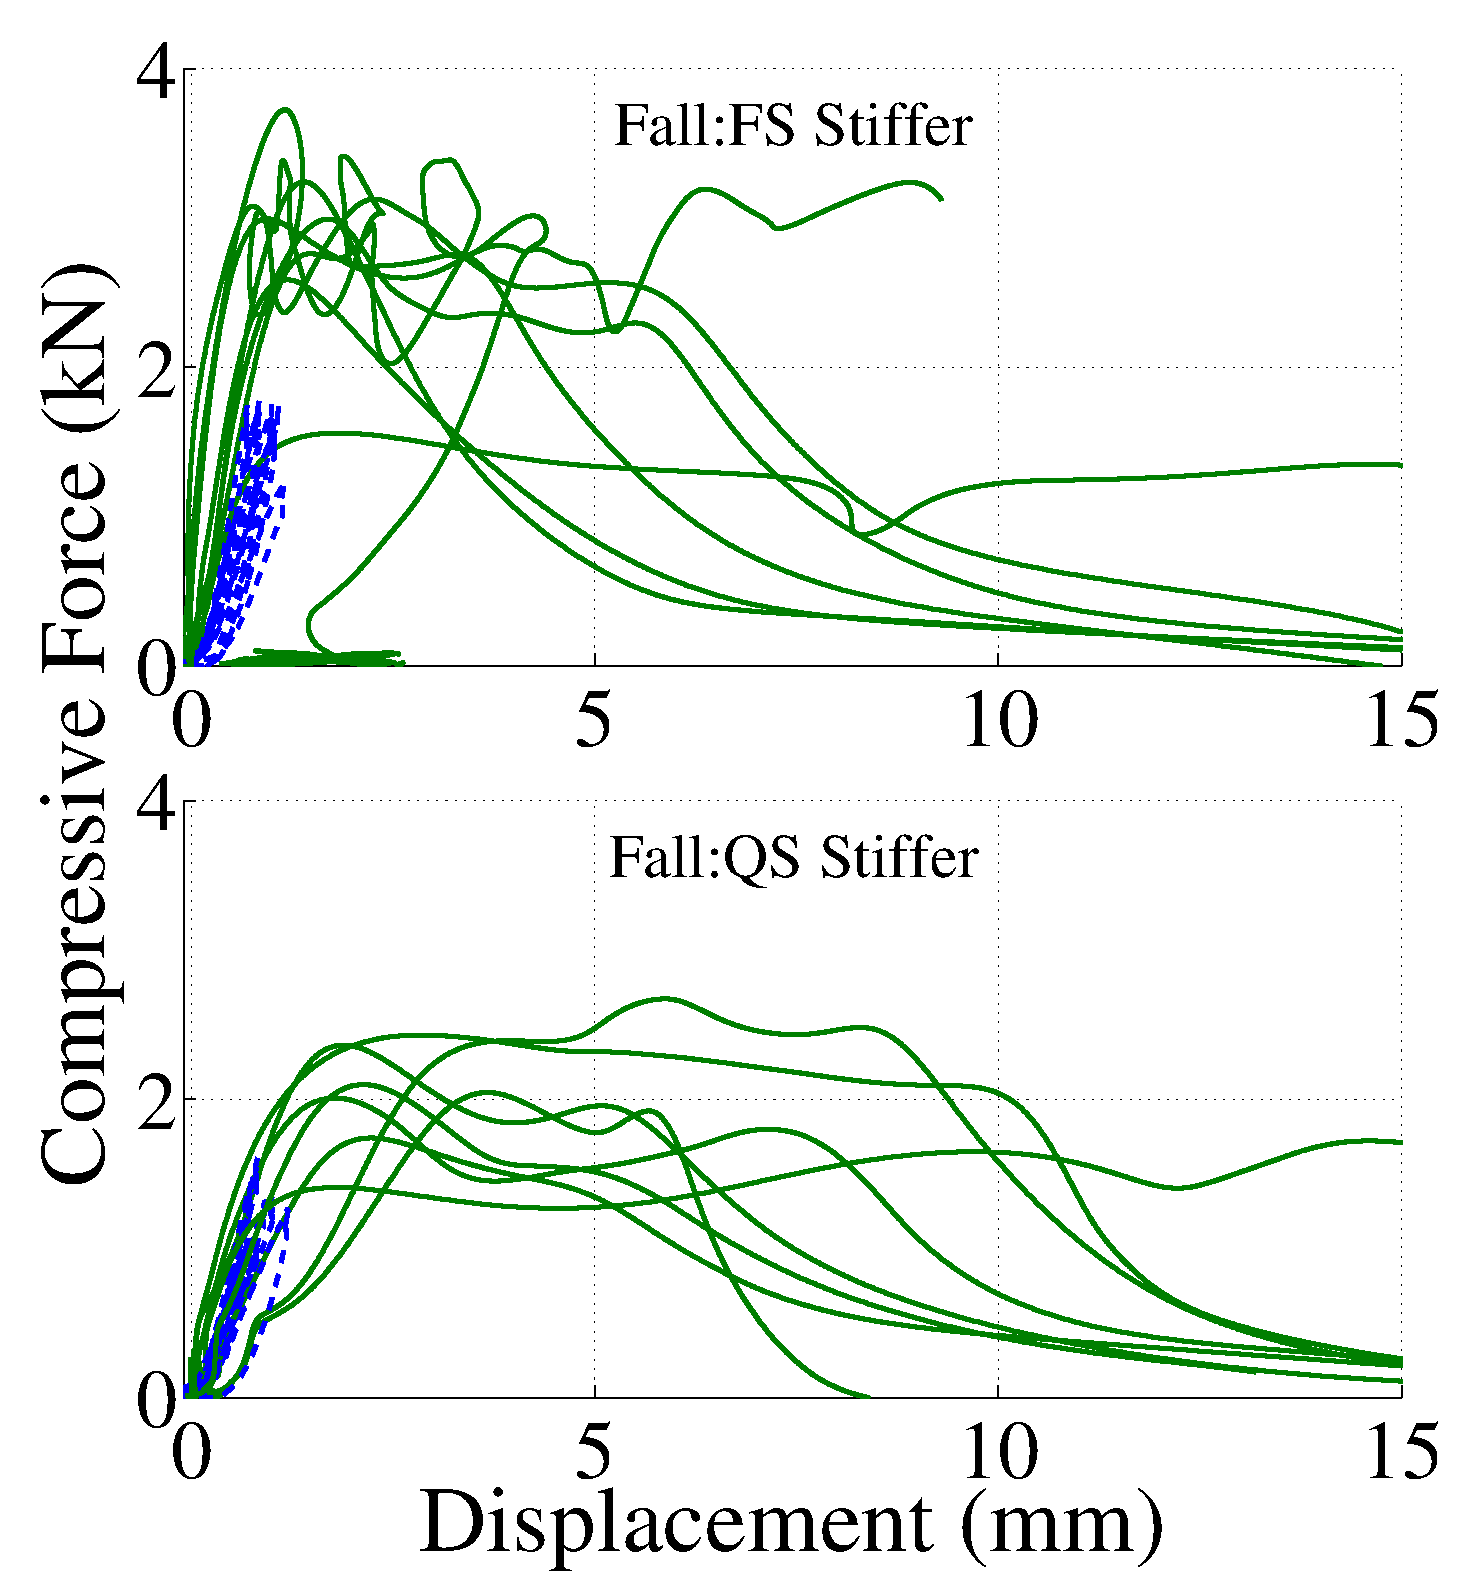
\includegraphics[width=\linewidth]{./behave_fail/Figures/Force_Disp_GroupedStiff}
\caption[Force-displacement behaviours grouped by relative stiffness of fall:\acs*{fs} and fall:\acs*{QS}]{
\textbf{Force-displacement curves for specimens, grouped by relative behaviour in the \ac{fs} and \ac{QS} conditions. Those that were stiffer in the \ac{QS} condition failed at a lower force, but displayed extended post yield behaviours. Dashed blue lines show the \ac{QS} loading response, and solid green lines are the \ac{fs} response.} Graphic \copyright Seth Gilchrist, 2013.}
\label{fig:Force_Disp_GroupedStiff}
\end{figure}

Yield force, stiffness and energy to fracture in the fall:\ac{fs} group were all significantly different from fast group (Table~\ref{tab:failData}).
The fall:\ac{fs} group was 24\% weaker, 160\% stiffer, and absorbed only 27\% of the energy before yielding.

\begin{table}
\centering
\begin{threeparttable}
\caption[Data for failure groups]{Data from the fall:\ac{fs}, fast and slow failure groups given as median (minimum, maximum) for non-normal data, and mean (standard deviation) for normally distributed data.}
\label{tab:failData}
\begin{tabular}{lccc}
\toprule
Measure 					& Fall:\ac{fs} 			& Fast				& Slow 					\\ \midrule
Yield Force (\ac{n})			 	& 2.39 (1.41, 3.72)	& 3.15 (2.17, 5.30)\tnote{*}	& 2.42 (1.46, 4.44)		\\ 
Stiffness (\ac{kn}/\ac{mm}) 			& 1.92 (1.20) 		& 0.74 (0.25)\tnote{*} 		& 1.66 (0.52)	 		\\ 
Energy (\acs{j}) 					& 2.55 (0.545, 5.39)& 9.33 (5.46, 15.4)\tnote{*}	& 4.38 (1.14, 12.2)\tnote{*}		\\
\bottomrule
\end{tabular}
\begin{tablenotes}
\item[*]{\footnotesize $p \leq 0.01$ compared to fall:\ac{fs}}
\end{tablenotes}
\end{threeparttable}
\end{table}

Energy in the fall:\ac{fs} group was significantly different from the slow group, absorbing only 58\% of the slow group's average before yield, but no differences were observed in yield force (\ac{pw}$ = 0.85$) or stiffness (\ac{pt}$ = 0.82$).

\begin{figure}
\centering
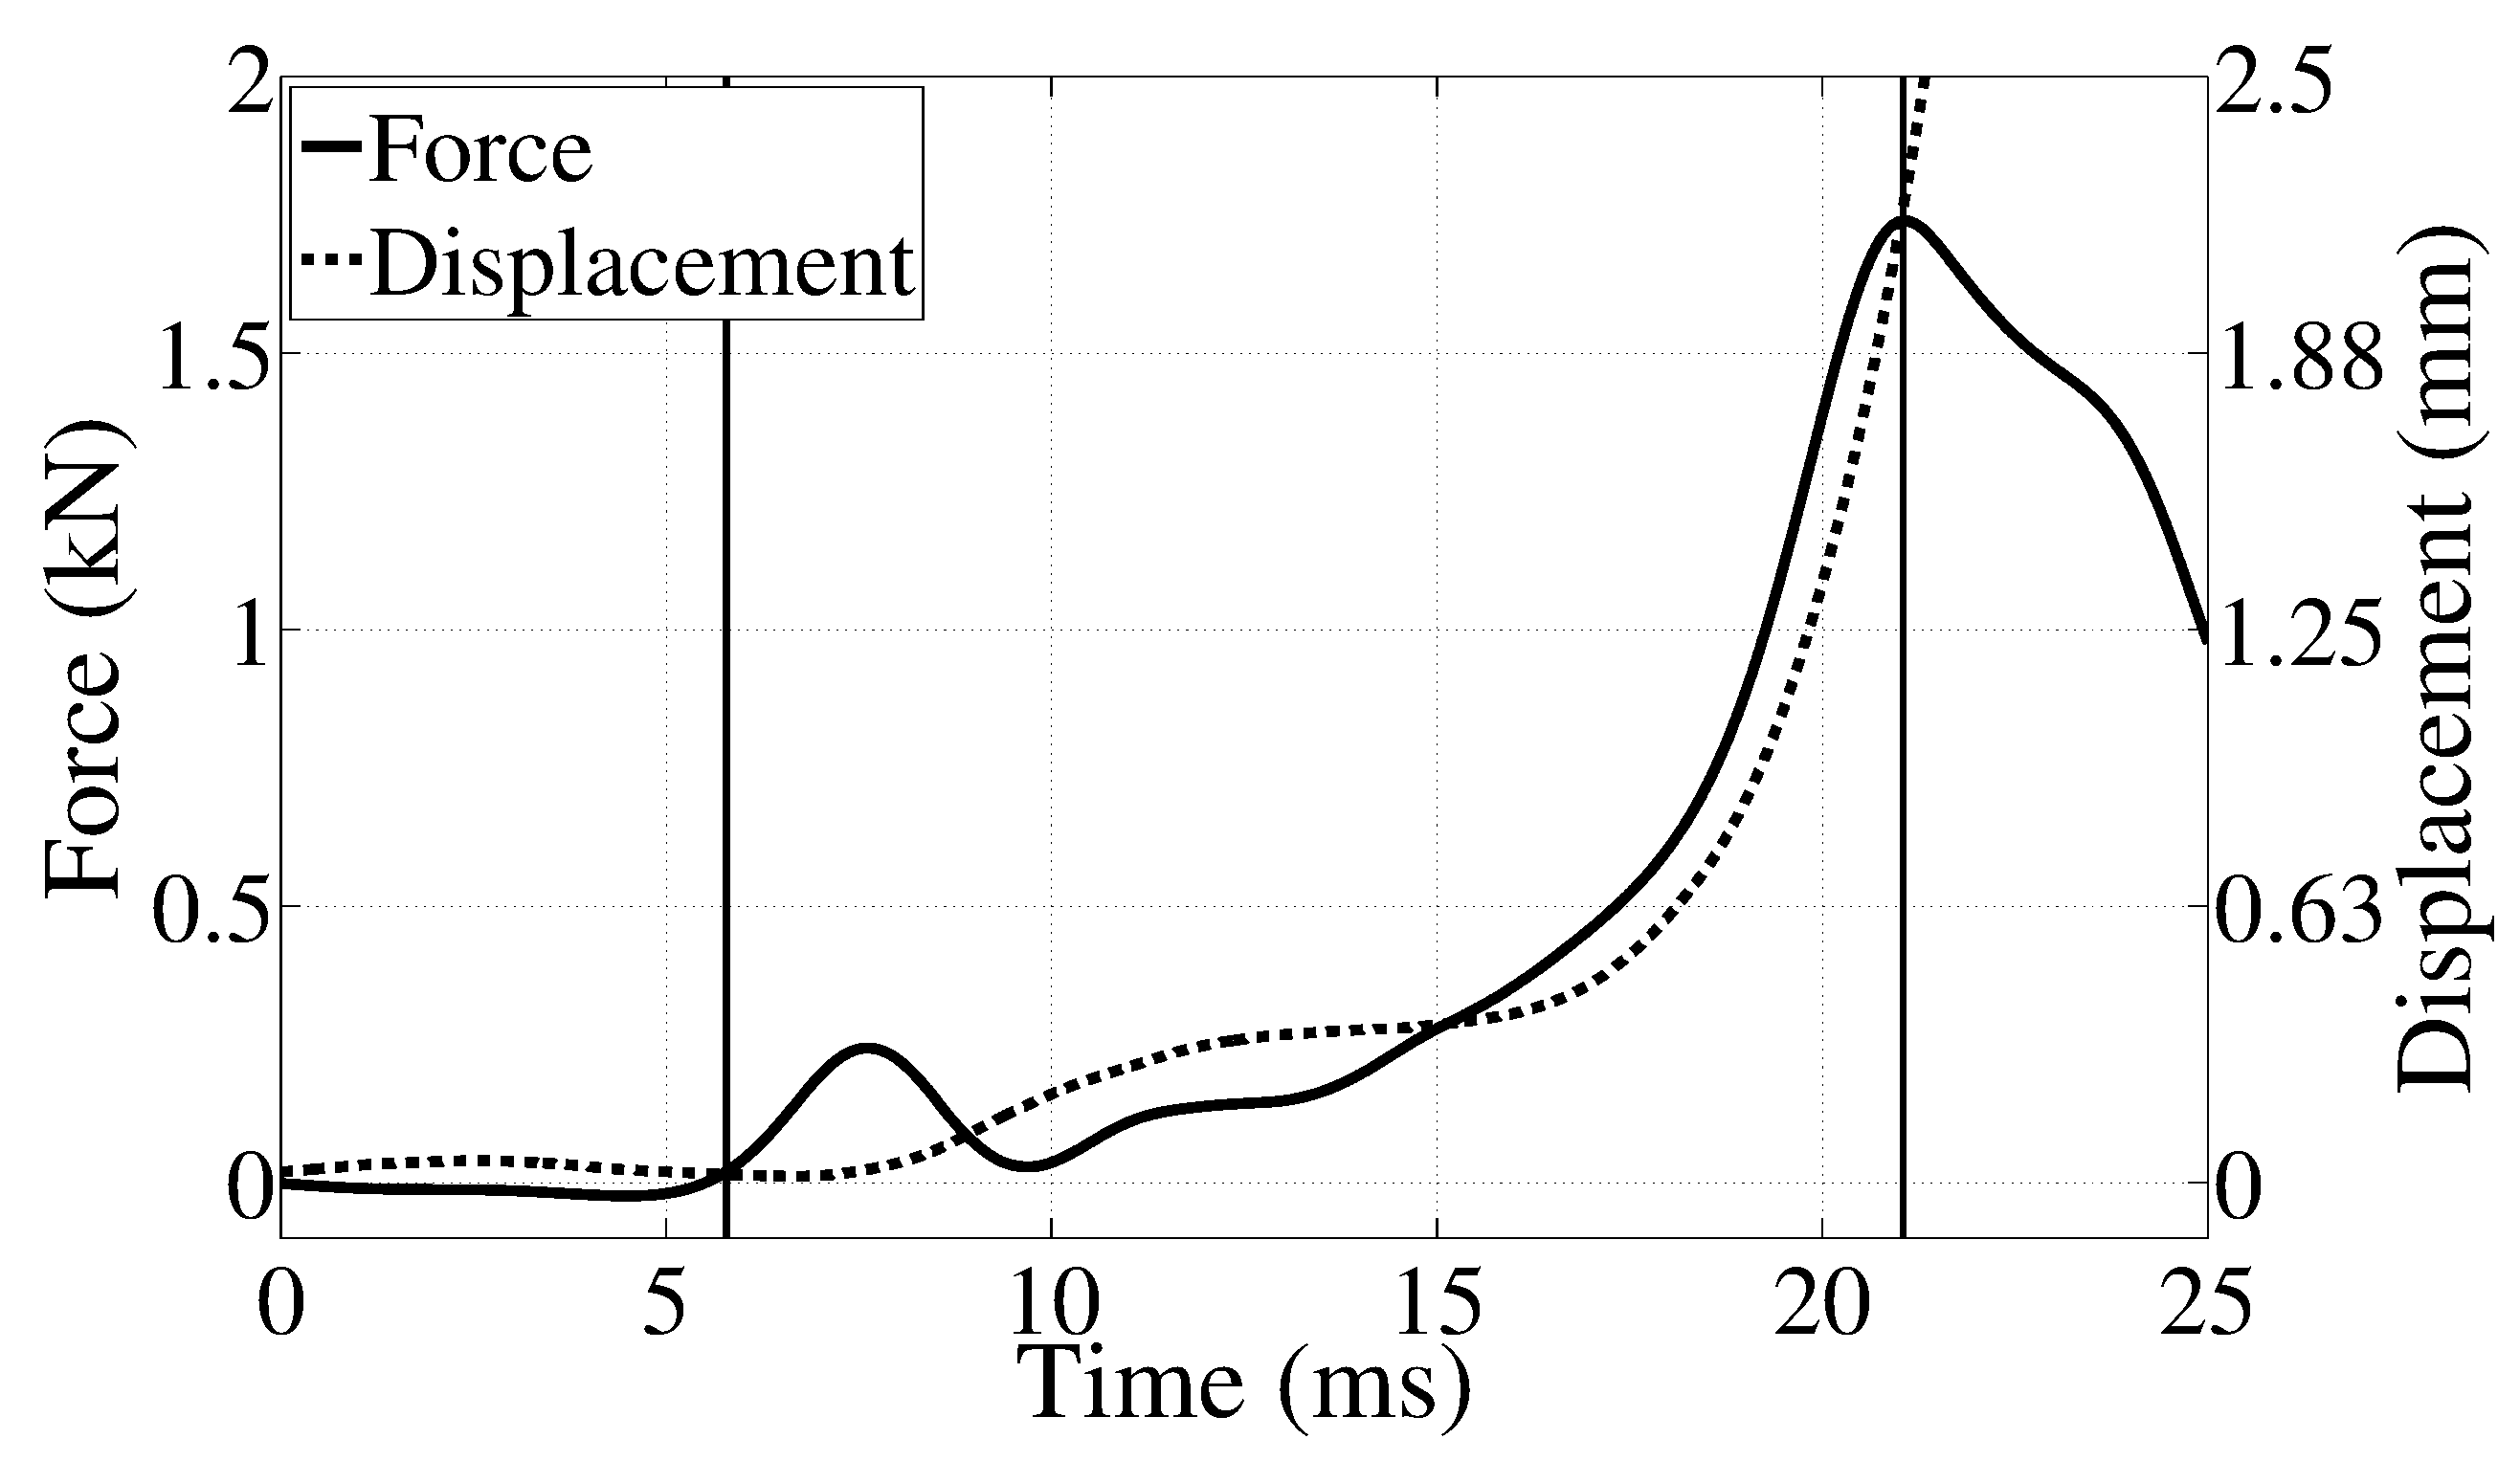
\includegraphics[width=\linewidth]{./behave_fail/Figures/Force_Disp_TimeExp}
\caption[Force and displacement \acs*{vs} time example]{\textbf{An example force and displacement \ac{vs} time plot. The vertical lines indicate the beginning of the impact (force $>$ 20~\ac{n}) and yield. Loading rate was defined as the average slope of the force-time curve from when the force exceeded 20~\ac{n} to yield. Likewise, displacement rate was the average slope of the displacement-time curve from when the force exceeded 20~\ac{n} to yield. These data are for specimen 7 and display the non-constant loading and displacement rates.} Graphic \copyright Seth Gilchrist, 2013.}
\label{fig:Force_Disp_TimeExp}
\end{figure}

The fall:\ac{fs} group displayed a variety of loading and displacement rates, both of which correlated with specimen stiffness (Table~\ref{tab:summary} and Figs.~\ref{fig:Force_Disp_TimeExp},~\ref{fig:StiffVsRate_HighRes} and~\ref{fig:Force_DispExp}).
As stiffness increased, loading rate increased (\ac{pt}$ < 0.01$) and displacement rate decreased (\ac{pt}$ < 0.01$).
Additionally, stiffness and yield force were proportionally related (\ac{pt}$ < 0.01$, \ac{r2}$ = 0.391$).
Finally, loading rate was correlated to maximum force (\ac{r2}$ =0.92$, \ac{pt}$ < 0.001$), but no correlation with displacement rate was observed (\ac{pt}$ = 0.16$).

\begin{figure}
\centering
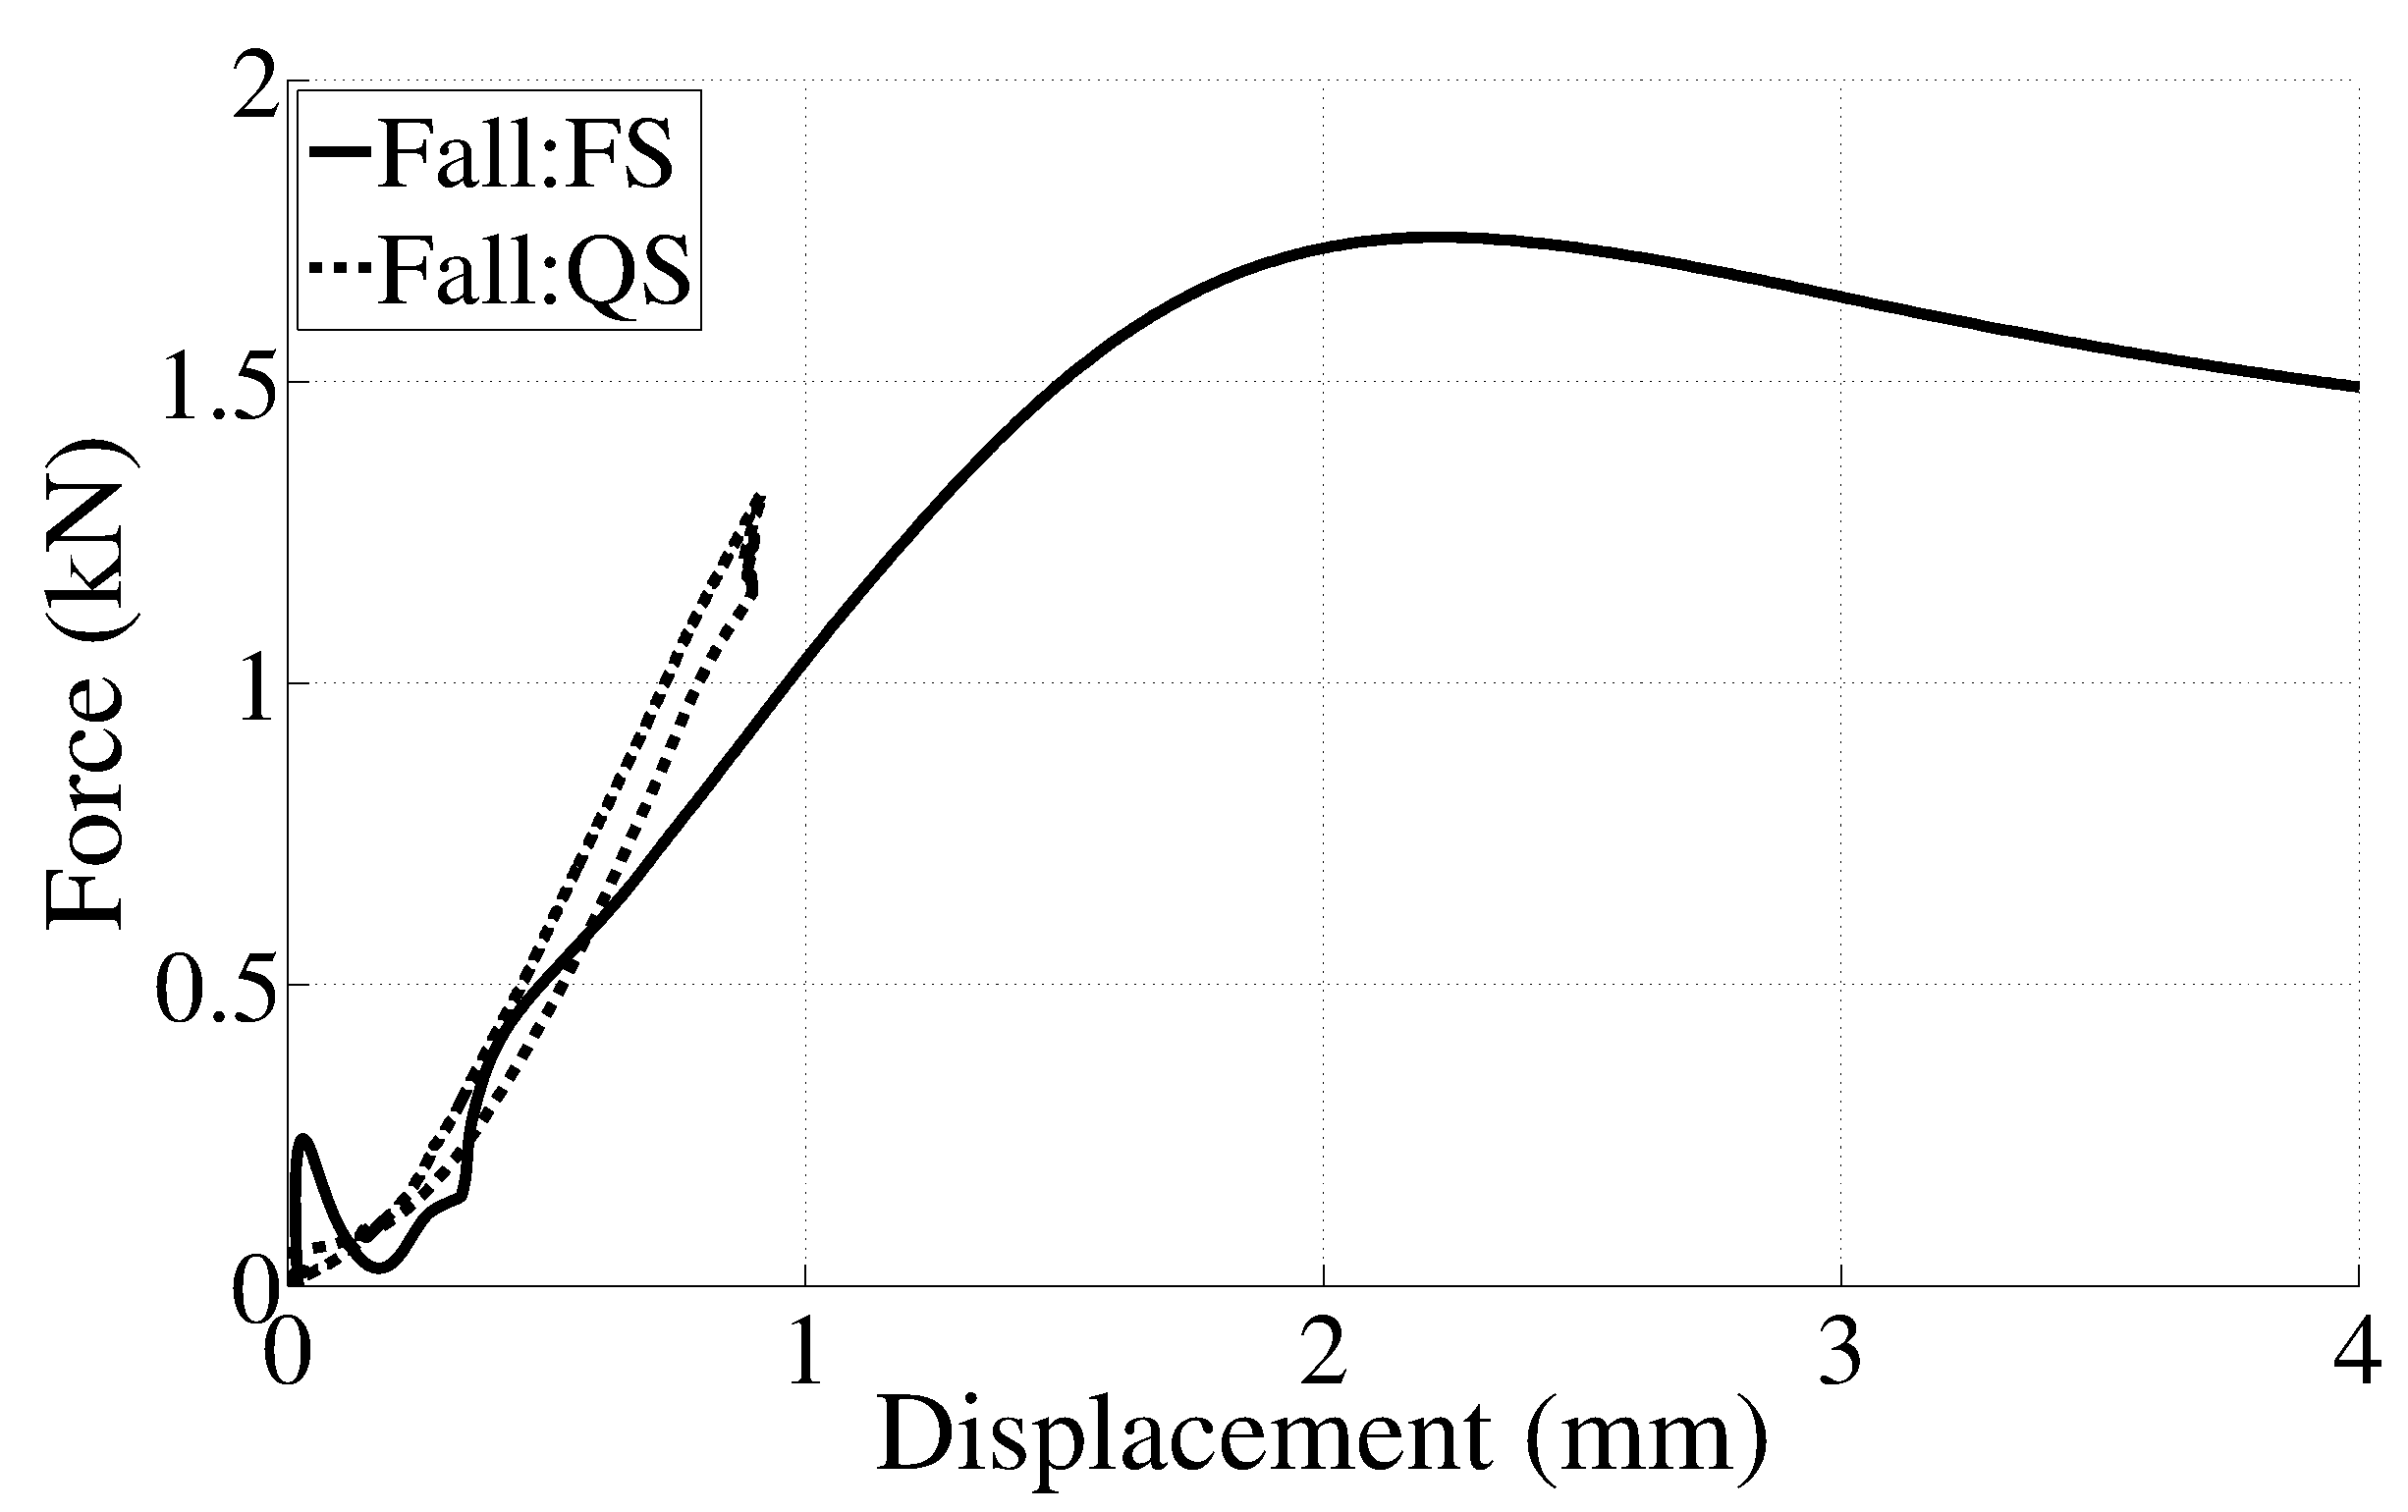
\includegraphics[width=\linewidth]{./behave_fail/Figures/Force_DispExp}
\caption[Force \acs*{vs} displacement example]{\textbf{An example force \ac{vs} displacement plot. In this case the quasi-static test had a higher stiffness than the fall simulation. These data are for specimen 7.} Graphic \copyright Seth Gilchrist, 2013.}
\label{fig:Force_DispExp}
\end{figure}

\begin{figure}
\centering
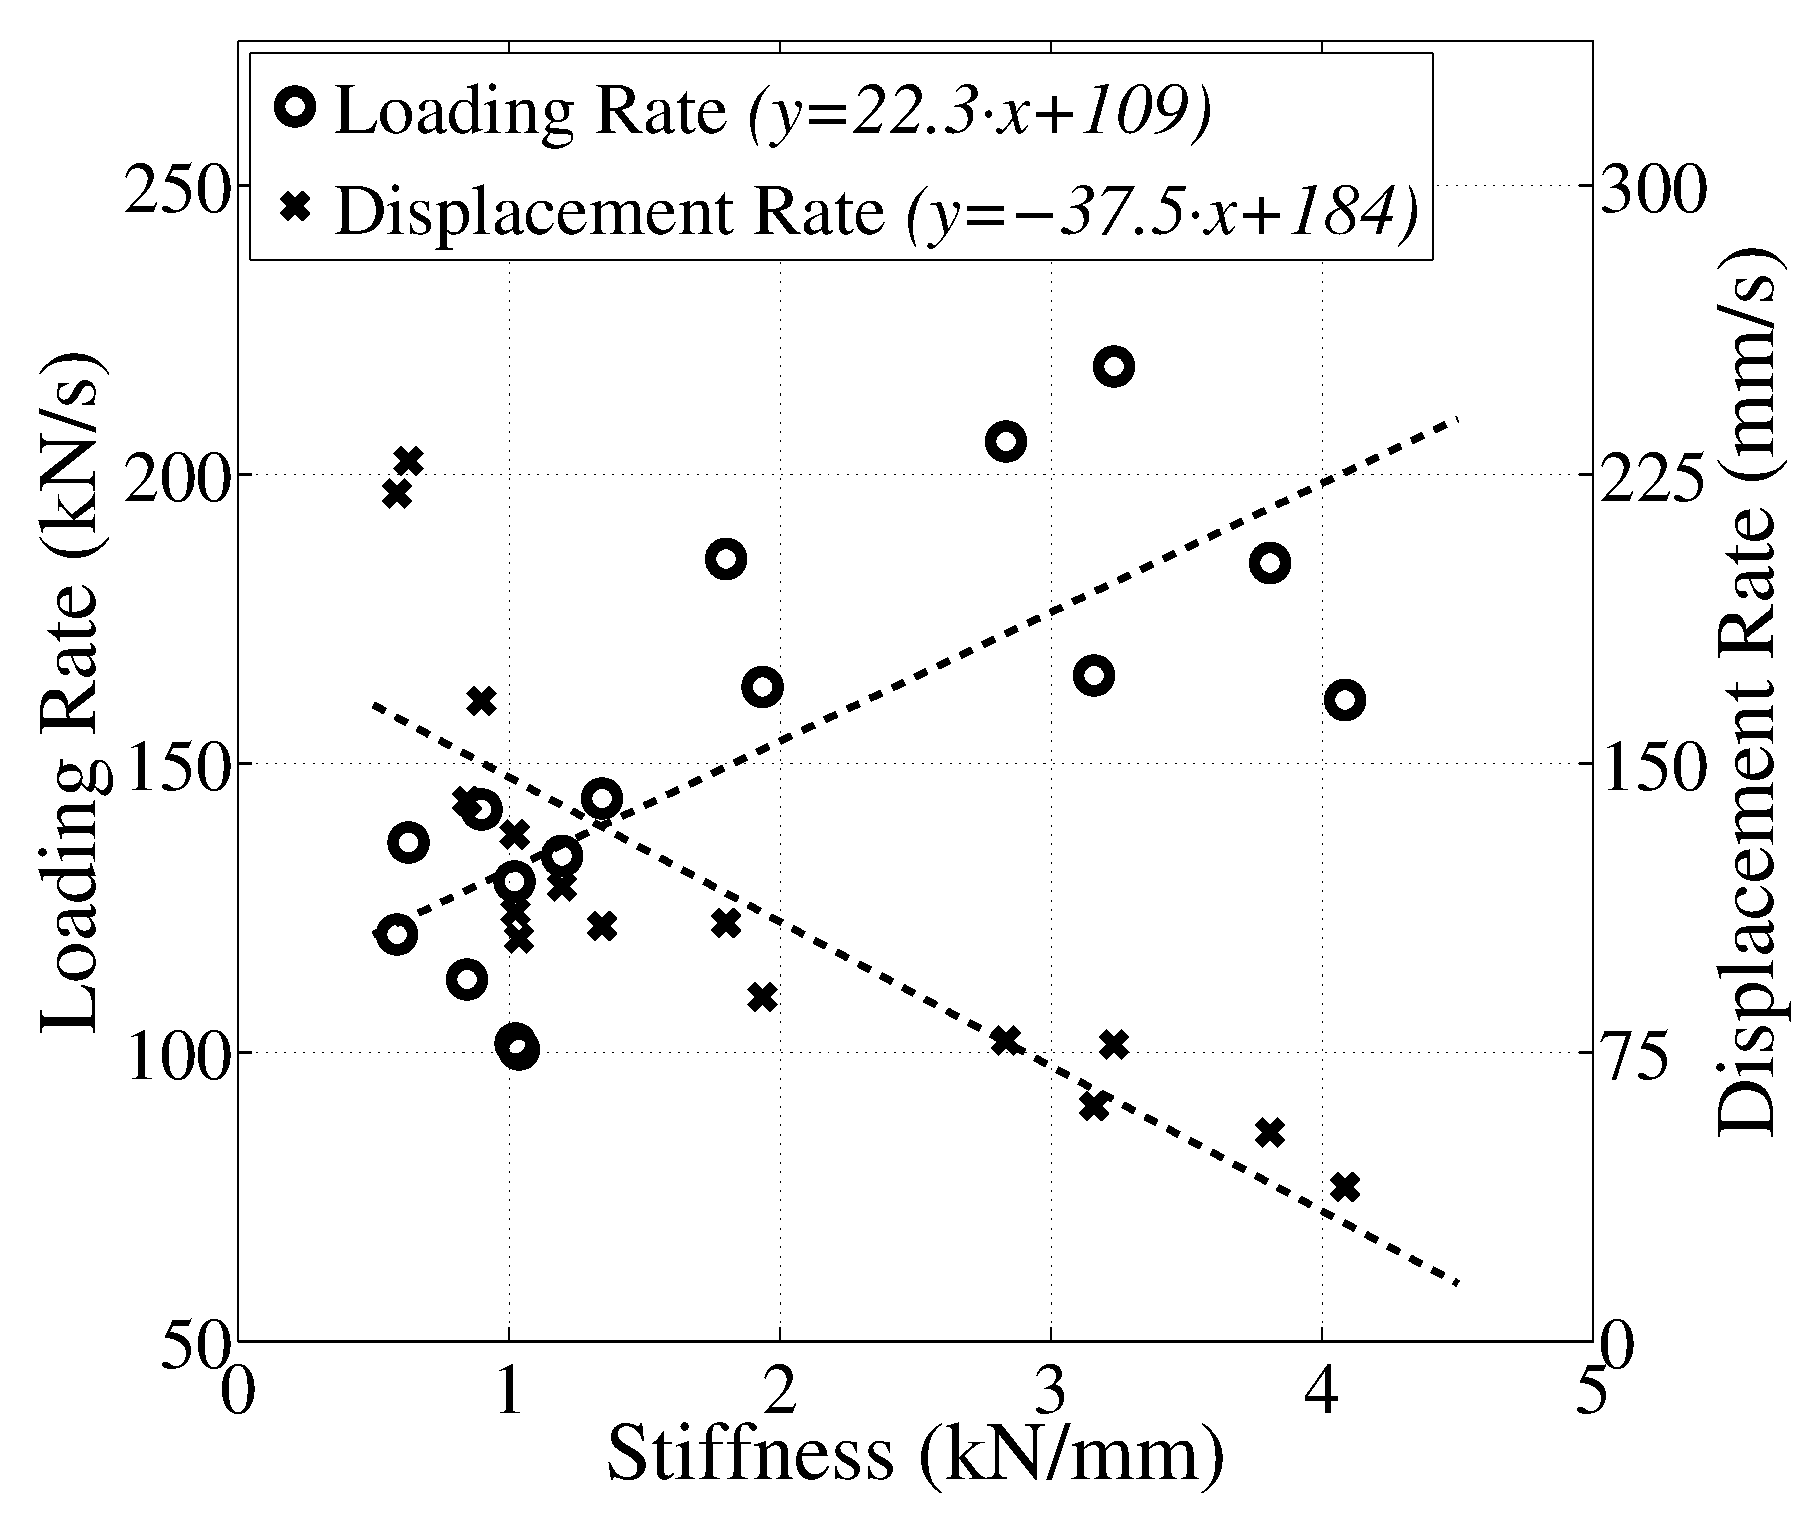
\includegraphics[width=\linewidth]{./behave_fail/Figures/StiffVsRate_HighRes}
\caption[Stiffness \acs*{vs} loading and displacement rates]{\textbf{Fall:\ac{fs} loading and displacement rates as functions of stiffness. Data points and regression lines for loading rate (\ac{r2}$ = .53$), and displacement rate (\ac{r2}$ = 0.66$) are shown.} Graphic \copyright Seth Gilchrist, 2013.}
\label{fig:StiffVsRate_HighRes}
\end{figure}

There were no differences in the slopes of the yield force \ac{vs} total \ac{abmd} regression lines between the fast, slow and fall:\ac{fs} groups (\ac{pt}$ = 0.88$ and \ac{pt}$ = 0.46$ for \citet{de_bakker_during_2009} and \citet{nishiyama_proximal_2013}, respectively). 

\section{Discussion}
\label{sec:behave_fail_discssion}
The goals of our experiments were three fold: i) to determine if there were differences in behaviour between quasi-static, constant displacement rate and fall simulation loading conditions; ii) to determine if there were differences in failure characteristics between constant displacement rate loading and fall simulation; and iii) to characterize the variation in loading and displacement rates as a function of specimen stiffness in the fall simulation tests.
Our fall:\ac{QS} \ac{vs} fall:\ac{fs} results dictate that we accept the null hypothesis that the sub-failure mechanical behaviour is the same between these test conditions.
However, the results of the constant displacement rate failure \ac{vs} fall simulation failure loading showed significant differences, requiring us to reject the null hypothesis of no difference between quasi-static and impact fall simulation failure characteristics.
In the fall simulation tests we found that the average displacement rate decreased with specimen stiffness, while the average loading rate increased.

\subsection{Fall group viscoelasticity}
\label{sec:behave_fail_discssion_relating}
The lack of differences in the fall:\ac{QS} \ac{vs} fall:\ac{fs} strain, energy and stiffness data is in contrast to previous work in hip fracture~\citep{weber_proximal_1992, courtney_effects_1994}, and could be seen to run counter to studies that have shown that bone, as a material, is viscoelastic~\citep{fois_study_2001, carter_compressive_1977}.
However, studies examining bone have shown that the viscoelastic effects are limited, and if bone viscoelasticity alone were responsible for the increase in stiffness seen by \citet{courtney_effects_1994}, the change in stiffness from 2 to 100~\ac{mm}/\ac{s} would be on the order of 25\%, rather than the 100\% observed.
The result in this study of increased \ac{abmd} being predictive of changes in stiffness could indicate that bone marrow space, which is presumably less in specimens with more trabecular bone, might be responsible for the changes in stiffness.
The material level studies suggest that the viscoelastic response of bone is connected to the organic matrix present~\citep{fois_study_2001}, which is unknown for the current specimen groups, and to hydrodynamic effects of bone marrow at high strain rates~\citep{carter_compressive_1977}.
In the fall simulation tests, the displacement rates were lower at the beginning of the test than at the end (Figure~\ref{fig:Force_DispExp}), but were still two orders of magnitude higher than for the fall:\ac{QS} group.
Therefore, our results suggest that our specimens were not exhibiting strong viscoelastic behaviour under these displacement rates, and this is the reason for the similar stiffnesses, energies and strains measured.

To examine the role of viscoelasticity, an idealized model (Figure~\ref{fig:ImpactModel}) was used to evaluate anticipated behaviours.
If the impact dynamics of the drop tower gantry and top of the spring are ignored, the initial velocity, $v(0)$, of Mass 1 can be calculated to be 2.9~\ac{m}/\ac{s} using energy methods (\S\ref{sec:support_mass1_velocity}).
The soft tissue model significantly influences the shape of the force pulse, $f(t)$, delivered to Mass 2 and since the soft tissue is omitted in this model, a representative sinusoidal pulse of 250~\ac{n} over 5~\ac{ms} $ \left( f(t) = 250 \sin(\frac{2\pi}{0.01} \cdot t)\right) $ was used.
If the damping of the proximal femur is given a value of 0, and the pelvis spring is given its laboratory measured stiffness of 50~\ac{kn}/\ac{m}, the response of the system is similar to that seen in the actual tests (Figs.~\ref{fig:StiffVsRate_HighRes} and~\ref{fig:stiffVsRatesIdeal}). Computer code for this model can be found in \S\ref{sec:code_ideal_fs}.

\begin{figure}
\centering
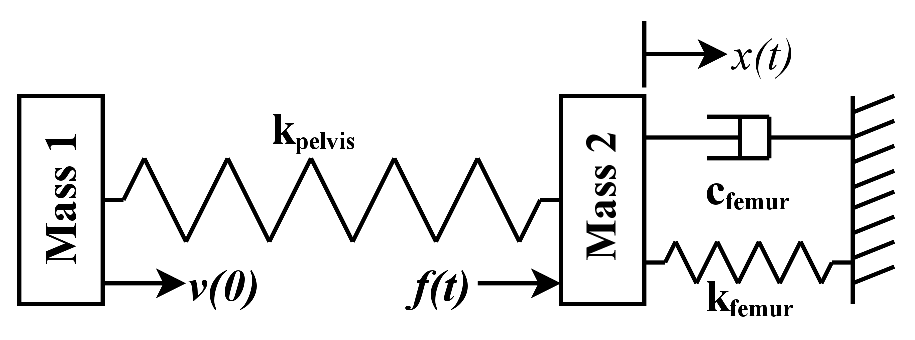
\includegraphics[width=\linewidth]{./behave_fail/Figures/ImpactModel}
\caption[Idealized model of the fall simulator]{\textbf{The impact fall simulator can be idealized using a series of two springs. This model is a 2~degree of freedom, second order model. It omits the soft tissue and models the pelvis spring as an ideal spring, and the femur as a spring and damper in parallel. Mass 1 is the combination of the body mass and the top third of the spring mass, and Mass 2 is the combination of the apparatus, bottom third of the spring, and the pelvis mass.} Graphic \copyright Seth Gilchrist, 2013.}
\label{fig:ImpactModel}
\end{figure}

\begin{figure}
\centering
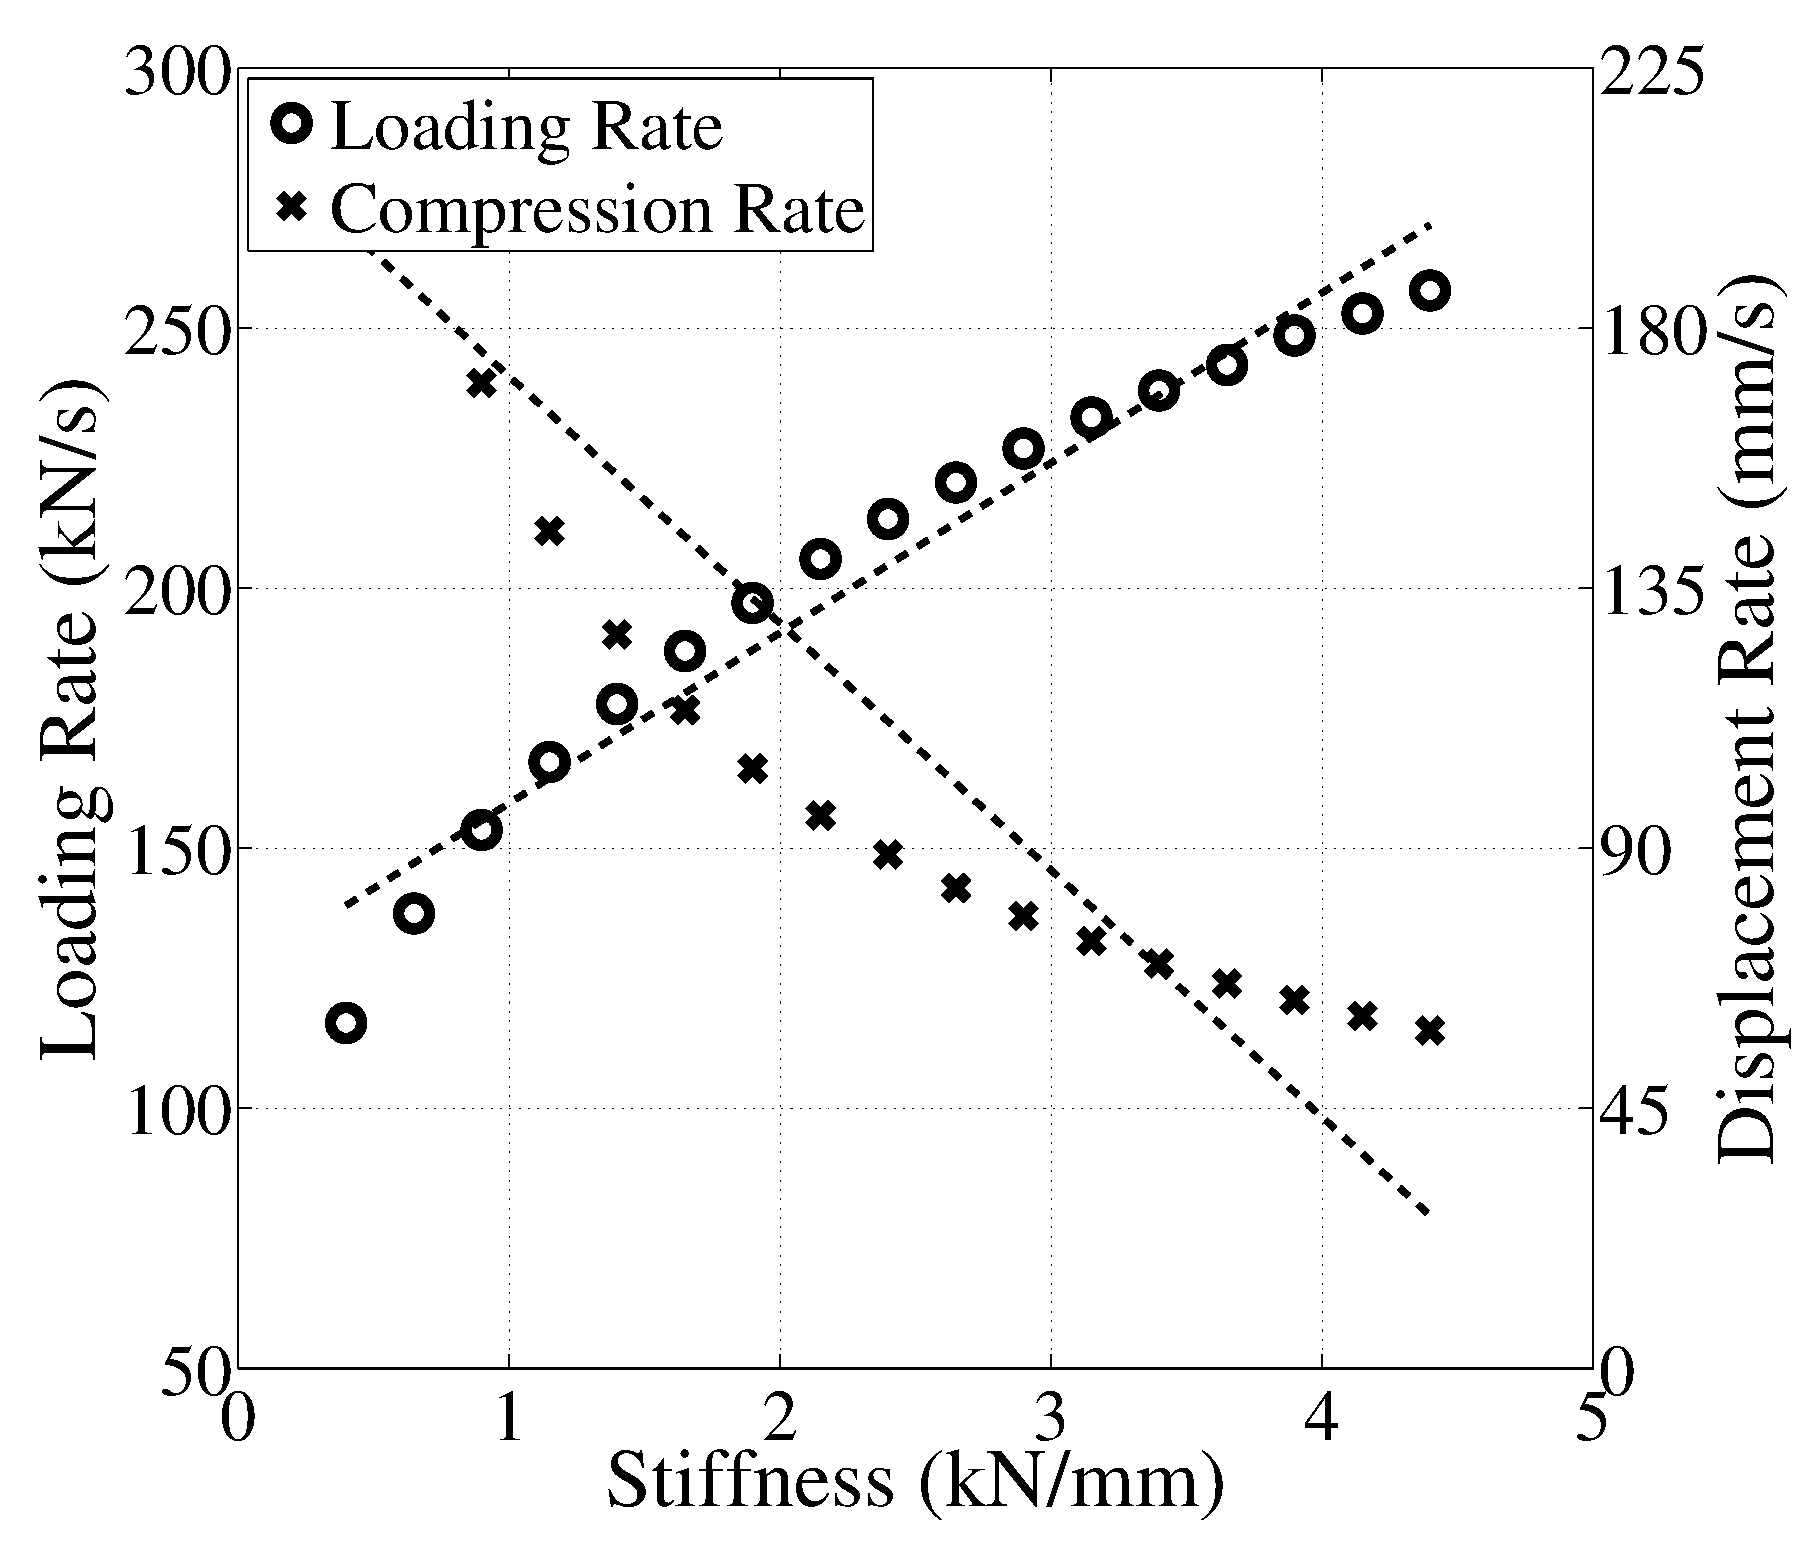
\includegraphics[width=0.7\linewidth]{./behave_fail/Figures/stiffVsRatesIdeal}
\caption[Ideal loading and compression rates \acs*{vs} stiffness]{\textbf{A plot for comparison to Figure~\ref{fig:StiffVsRate_HighRes} that shows the loading and compression rates \ac{vs} stiffness for an ideal spring-mass system up to 1500~\ac{n} of compressive force. The trend lines in this plot behave in the same manner to those in the experimental data, indicating that the system is behaving in a spring-like fashion.} Graphic \copyright Seth Gilchrist, 2013.}
\label{fig:stiffVsRatesIdeal}
\end{figure}

The question then becomes, what would the system look like if damping was increased, simulating high bone viscoelasticity?
The same model as above was used, however the force on Mass 2 was omitted because oscillations due to the force pulse were seen to dominate loading and displacement \ac{vs} stiffness plots at high damping levels.
Since none of the specimens were fractured by the initial force pules, the artefact created by it would obfuscate the important signals in the plots.
Therefore, the initial conditions were set to $v(0) = 2.9$~\ac{m}/\ac{s} and $f(0) = 0 $, and a number of different damping values were tested (Figure~\ref{fig:ratesVsDamping}).

\begin{figure}
\centering
\includegraphics[width=\linewidth]{./behave_fail/Figures/ratesVsDamping}
\caption[Ideal loading and displacement rates as a function stiffness and damping]{\textbf{Loading and displacement rates \acs{vs} stiffness, plotted for four different damping levels. The number in the upper left of each plot gives the value of $c_{femur}$.} Graphic \copyright Seth Gilchrist, 2013.}
\label{fig:ratesVsDamping}
\end{figure}

Increased damping has a large effect on the shape of the displacement rate curve, tending to flatten it out and decrease its overall value.
This shape change is due to the viscous element preventing compression of the spring element.
In specimens with low stiffness velocity tends to increase rapidly in the absence of damping, leading to high displacement rates.
However, in situations where the viscous response dominates, high compressions are never achieved.
Increasing the damping decrease the value of the loading rate curve and, at higher damping levels, flattens out the response.
This flattening of the load and displacement rate curves at high damping levels occurs because the system is over damped.
In the over damped scenario, the loading rate tends towards a constant value, determined by the compression rate of the pelvis spring, and the displacement rate tends to a value of zero.

In the test results (Figure~\ref{fig:StiffVsRate_HighRes}) the loading rate fit line has a positive slope, and the displacement rate fit line has a negative slope, leading us to draw the conclusion that viscoelastic response is likely minimal.

So how does this fit in with the work of \citet{courtney_effects_1994}?
The change in stiffness reported by \citet{courtney_effects_1994} for old femurs was an increase of 92\% when increasing the displacement rate from 2~to 100~\ac{mm}/\ac{s}.
These data can be used to estimate the damping coefficient of their specimens.
Modelling the system used by \citet{courtney_effects_1994} as a spring and damper in parallel, driven by a constant displacement rate (Figure~\ref{fig:courtneyModel}), we can estimate the damping coefficient needed to double the stiffness to a given compressive force (equations for this analysis cab be found in \S\ref{sec:support_courtney_response}).

\begin{figure}
\centering
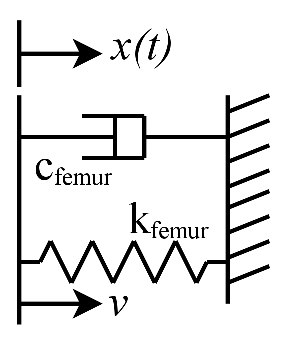
\includegraphics[width=0.3\linewidth]{./behave_fail/Figures/courtneyModel}
\caption[Idealized \citet{courtney_effects_1994} model]{\textbf{An idealized version of the test setup used by \citet{courtney_effects_1994}. The stiffness of the construct is the combination of the baseline femur stiffness and the resistance due to the damping.} Graphic \copyright Seth Gilchrist, 2013.}
\label{fig:courtneyModel}
\end{figure}

Using a baseline femoral stiffness of 1.5~\ac{kn}/\ac{mm} (which is similar to the 2~\ac{mm}/\ac{s} value measured by \citet{courtney_effects_1994}) and calculating the stiffness up to 2.4~\ac{kn} (the average strength of the current specimens) shows that to double the stiffness when displacement rate is changed from~2 to~100~\ac{mm}/\ac{s}, the damping coefficient, c$_{femur}$ would need to be approximately 12~\ac{n}\ac{s}/\ac{mm} (Figure~\ref{fig:courtneyDamping}).
If, however, the bone was acting in accordance to the strain rate to the power of 0.047-0.06~\citep{carter_compressive_1977, linde_mechanical_1991, crowninshield_response_1974}, the corresponding damping coefficient would be approximately 5~\ac{n}\ac{s}/\ac{mm}.

\begin{figure}
\centering
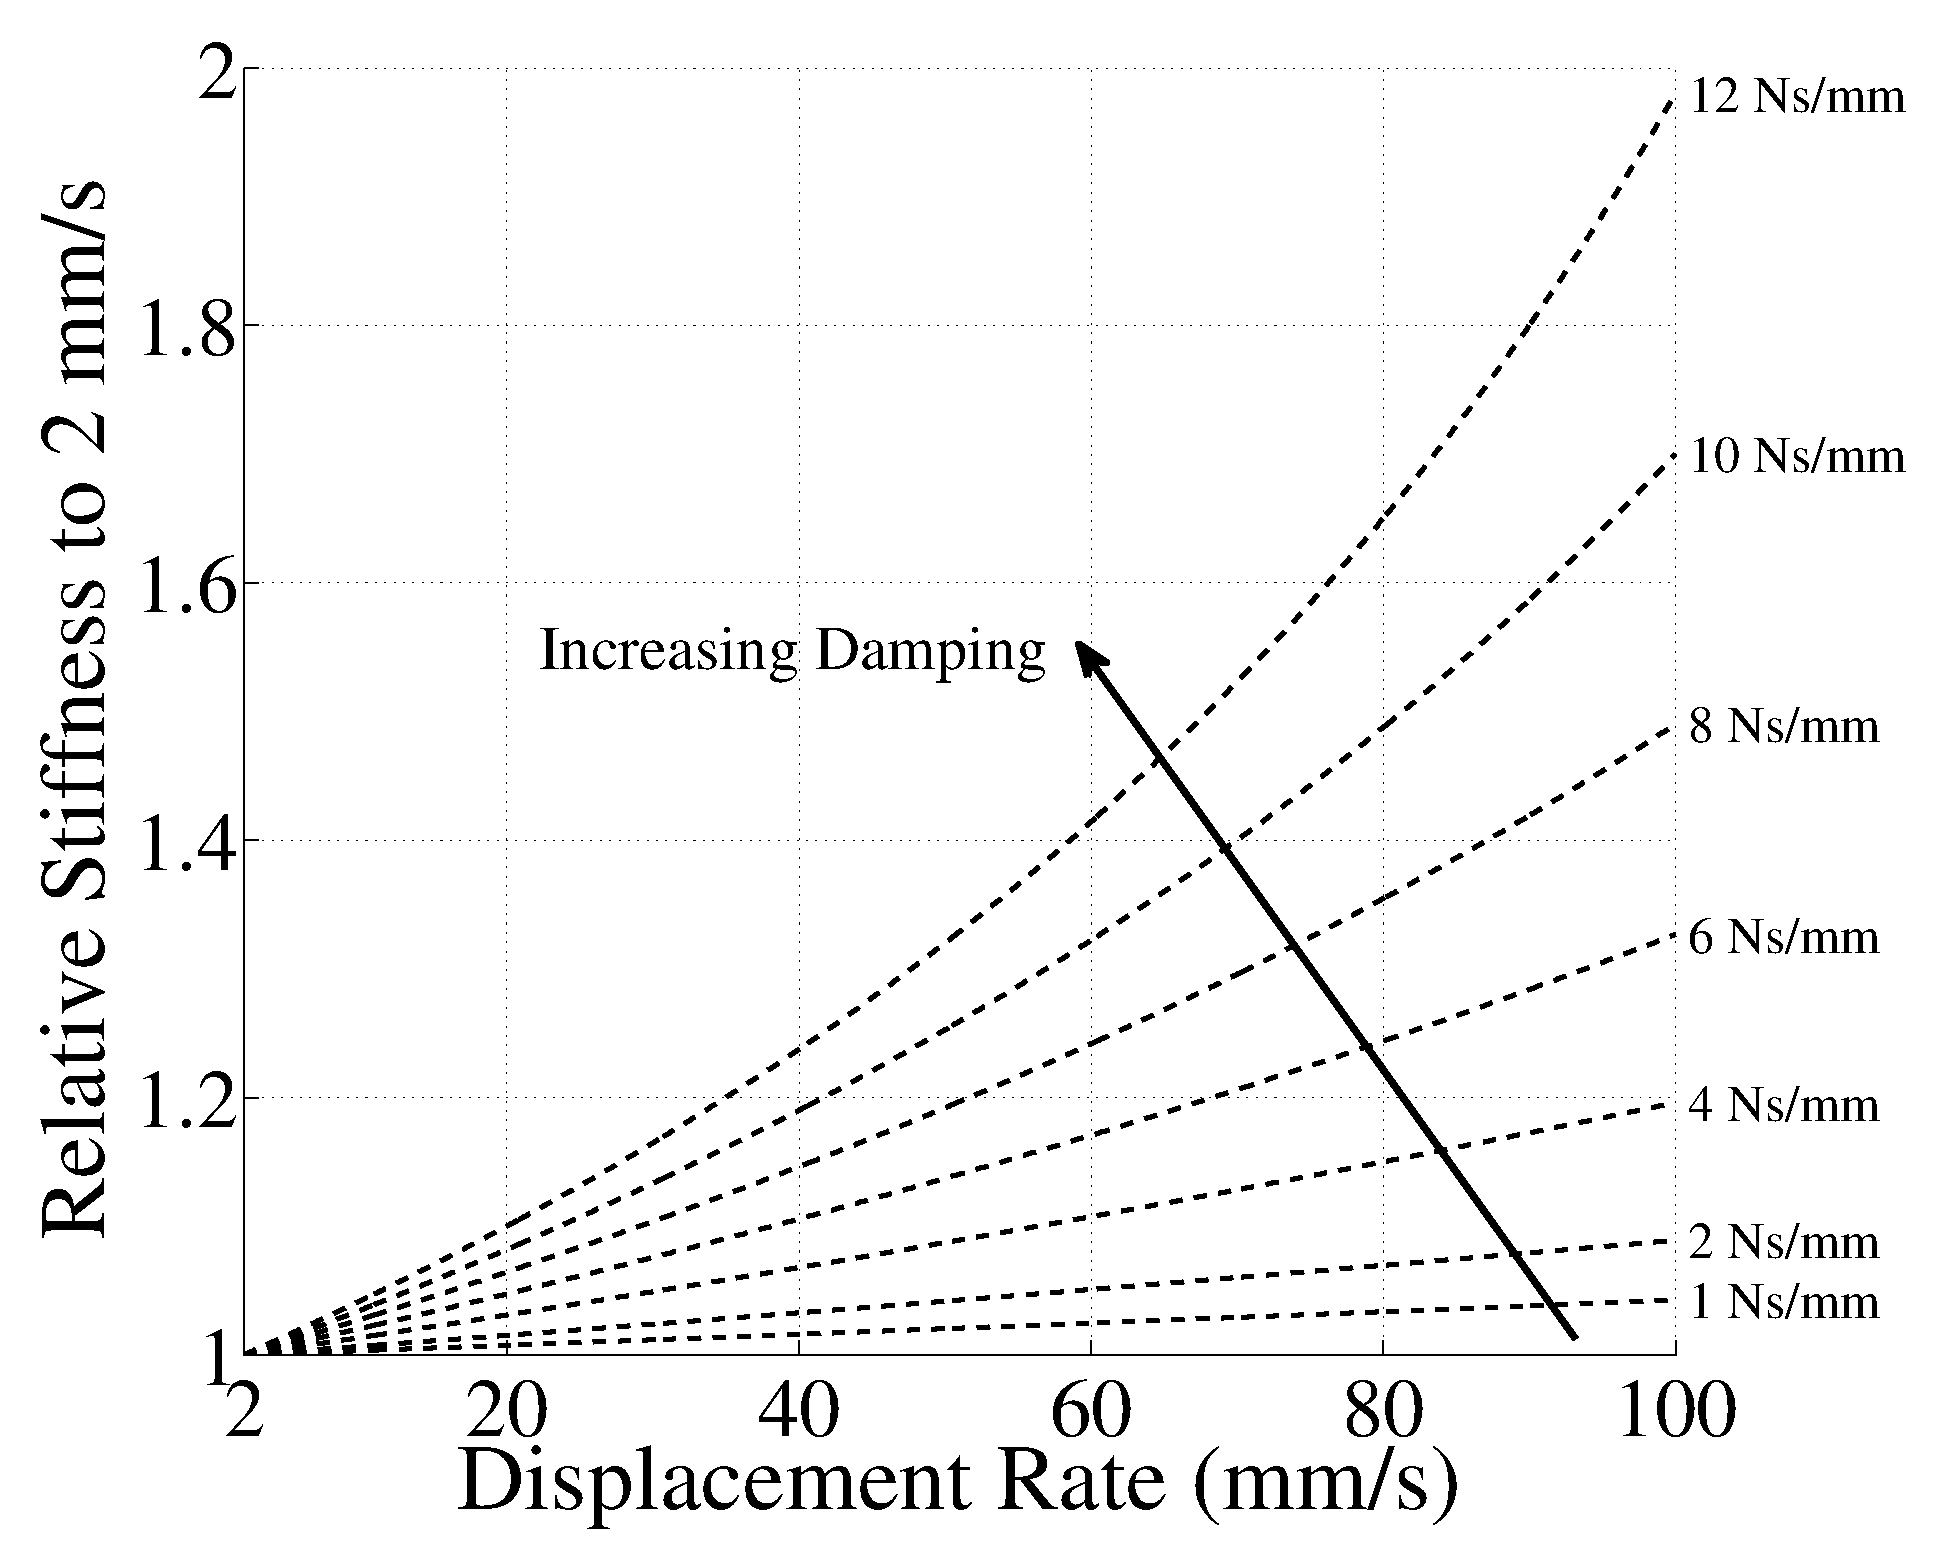
\includegraphics[width=0.7\linewidth]{./behave_fail/Figures/courtneyDamping}
\caption[Stiffness \acs*{vs} displacement rate and damping]{\textbf{Stiffness relative to the 2~\ac{mm}/\ac{s} value as displacement rate increases for various damping coefficients. Relative stiffness was calculated to a force of 2.5~\ac{kn}. Selection of target force or target displacement is important as it changes the nature of the relationship} (\S\ref{sec:support_courtney_response}). Graphic \copyright Seth Gilchrist, 2013.}
\label{fig:courtneyDamping}
\end{figure}

Returning now to the model of the current experiment, it can be seen that if the bone viscoelasticity was on the order of 5~\ac{n}\ac{s}/\ac{mm}, as proposed by \citet{carter_compressive_1977}, \citet{linde_mechanical_1991} and \citet{crowninshield_response_1974}, then it might be difficult to determine if the specimens in the current tests are acting with that level of viscoelasticity.
The model's displacement rate has a distinct negative slope, as does the experiment's, and there is considerable variation in the experiment's loading rate values, which might hide a lower slope than the fit line, similar to the model's.
However, if the specimens are acting with the level of viscoelasticity noted by \citet{courtney_effects_1994}, then one might anticipate nearly constant displacement and loading rates for all specimens, regardless of their baseline stiffnesses.
\citet{courtney_effects_1994} saw that young specimens with a higher baseline stiffness also doubled their stiffness at the higher displacement rates, indicating that their results were consistent regardless of baseline stiffness.
From this, we can conclude that the specimens may have some viscoelastic behaviour, but in the current tests it is not strong enough to heavily influence the response.

\subsection{Failure and loading responses in the fall simulator}
\label{sec:behave_fail_discssion_fail}
The fall:\ac{fs} group was significantly different from the fast group in every measure.
In absolute value terms the yield force was not much different, but the low stiffness in the fast group meant that the energy absorbed was higher.
The mechanism for these differences is not known, but the lower stiffness and higher yield force are incongruent with anticipated viscoelastic effects.

A central result of the study was observation of the variable nature of displacement and loading rates during a fall to the side.
Previous investigators have evaluated the effects of displacement rate by testing specimens to failure under multiple, fixed displacement rates~\citep{courtney_effects_1994, weber_proximal_1992}.
A consequence of fixing the displacement rate is that all specimens, even the stiff ones, are exposed to high loading rates.
The average stiffness from \citet{courtney_effects_1994} of 3.0~\ac{kn}/\ac{mm} at 100~\ac{mm}/\ac{s}, results in a loading rate of 300~\ac{kn}/\ac{s}.
Previous researchers have estimated the peak loading rate in humans falling to the side to be approximately 100~\ac{kn}/\ac{s}~\citep{laing_characterizing_2010}.
The current tests include a compliant pelvis model which acted to mitigate extreme loading rates, leading to an average rate of 150~\ac{kn}/\ac{s}.
Enforcing a high displacement rate on specimens may reduce the biofidelity when compared to free response.
While loading rates of 300 and 100~\ac{kn}/\ac{s} are the same order of magnitude, the differences could affect specimen behaviour in ways that are difficult to predict given the complex geometry and bone material response~\citep{carter_compressive_1977, robertson_compressive_1978, linde_mechanical_1991, hansen_effect_2008, zioupos_microcracking_2008}.

In the fall:\ac{fs} group, displacement rate was related to stiffness, but not to yield force.
While a statistical relationship with yield force could not be found, this could be due to a lack of power since the post hoc power of the current experiment is only 0.28.
The inverse relationship between stiffness and displacement rate contradicts the outcomes of previous research~\citep{courtney_effects_1994, weber_proximal_1992}.
This is thought to be a result of the influence of specimen stiffness on the dynamic response.
In the dynamic situation that we studied, displacement rate is related to specimen stiffness, with softer specimens experiencing higher displacement rates, which is in agreement with the fundamental mechanics of an undamped, spring-mass system.
We believe that observations of previous researchers~\citep{courtney_effects_1994, weber_proximal_1992}, who noted an increase in stiffness as displacement rate increased, were potentially an artefact of the prescribed constant loading rates on the bones.

\subsection{Conclusions}
\label{sec:behave_fail_discssion_conclusions}
Our approach here is markedly different from previous hip fracture fall simulation tests and we believe that it incorporates important improvements over the previous test methods in terms of concordance between the loading situation in real world falls and those in the experiment.
Most importantly, the new test method produces both loading and displacement rates as outcome variables that are determined by the biomechanics of the fall and bone structural material properties, rather than dictating one of these parameters a priori.
Secondly, the use of the same specimen to test two different loading conditions improves statistical power to assess the differences in mechanical behaviours.

While the advantages of the current method are important, there are also limitations with respect to comparison to previous studies.
The lack of match pairs for failure mechanics comparison reduced our ability to show differences in failure behaviours.
However, comparisons were made to two populations of specimens that were similar to the current one.
Additionally, specimens were from a non-fracture population, which may reduce the ability to identify mechanics of bones that actually fracture due to a fall.
Further, only surface strain and force-displacement behaviours were assessed, with no insight into the internal mechanics and load sharing between cancellous and cortical bone.
This final point is best addressed through the use of computational modelling, which is currently on-going.
Notably, the finite element models are developed and validated using data from the fall:\ac{QS} group.
Once the models have been validated for sub-failure loading using that data (for which no differences were seen vis-a-vis the fall:\ac{fs} group), they will be extended to model the failures observed in the fall:\ac{fs} group.

This chapter has shown that the mechanical behaviour of the proximal femur is the same in quasi-static, constant displacement rate loading as it is in impact fall simulation.
However, it has also shown that prescription of a single displacement rate at the greater trochanter for all specimens is a simplification that could significantly alter the behaviour of the specimen and may have been responsible for the viscoelasticity observed by previous researchers.
The following chapter will address the strain and failure characteristics of the proximal femur in the two loading scenarios, addressing the last two research questions outlined in Section~\ref{sec:intro_goals_questions}.
%% This is the impactor results chapter for my UBC PhD Dissertation
%% The parent document is called thesis.tex

\chapter{Impact and constant displacement rate loading change the surface strain and fractures of the femur in sideways fall simulation}
\label{ch:fracture}
Knowledge of proximal femur fracture initiation and progression could increase the ability predict who will suffer a hip fracture.
Initial failure locations could be important in the effort to increase the sensitivity of hip fracture screening techniques.
If failures start in one location, or in proximity to a certain type of structure, it may be possible to develop protocols that target these areas and identify if known morphologies that may lead to structural deficiency exist.
Additionally, knowledge of how the initial failure location influences the final fracture type may allow screening for those who could be susceptible to the most serious types of fractures.

Previous researchers have investigated failure locations~\citep{de_bakker_during_2009} and fracture patterns~\citep{backman_proximal_1957, lotz_use_1990, weber_proximal_1992, courtney_effects_1994, pinilla_impact_1996, keyak_prediction_2001, lochmuller_mechanical_2002, bell_structure_1999} in proximal femurs loaded to failure in materials testing machines.
These researchers used constant displacement rate loading techniques, some at low rates (\textless5~\ac{mm}/\ac{s}), and some at high rates (100~\ac{mm}/\ac{s}), to model a fall to the side.
While it has been shown that increasing displacement rate from 2 to 100~\ac{mm}/\ac{s} has only a modest effect on the ultimate strength of the proximal femur~\citep{courtney_effects_1994}, there are two questions that remain unanswered.
First, does 100~\ac{mm}/\ac{s} represent a real fall to the side, and secondly does the deformation of the bone, initial failure location or fracture type change when loading protocol is changed?

In Chapter~\ref{ch:behave_fail} I investigated the first of these issues, and this chapter concentrates on the questions of how the bone deforms and fails in the quasi-static, constant displacement rate and the impact fall simulations protocols.
Chapter~\ref{ch:behave_fail} investigated what loading protocol was appropriate for mechanical behaviour outcomes of the proximal femur, this chapter will inform researchers of the best protocol for investigating physical damage outcomes.
In this chapter, I investigate the strain developed on the surface of the proximal femur, as well as the changes in failure locations and final fracture types, with testing protocol as the independent variable.

Fracture of the proximal femur is preceded by the development of strain within the bone.
To assess the difference in the strain of the bone in the quasi-static, constant displacement rate apparatus and those loaded in the fall simulator, the surface strains on the anterior-superior neck of single specimens were compared between the two test conditions using \acf{dic}.

Comparison of the failure of the bones in the two tests conditions were done based on initial failure location, as well as final fracture pattern.
To compare these outcomes, two groups of similar specimens were loaded to failure, one using a quasi-static, constant displacement rate protocol, and the other using impact fall simulation.
The failure locations and fracture patterns were compared using categorical values and comparative diagrams.

A version of this chapter will be submitted to Osteoporosis International. 

\section{Introduction}
Hip fracture is a major orthopaedic burden, with reported averages of 20\% of orthopaedic beds being continuously occupied by hip fracture patients~\citep{lyritis_epidemiology_1992, borissova_femoral_2011}.
For this reason, researchers have striven to understand how fractures happen, and how those susceptible to fracture could be better identified.
Many experimental and computational tools have been developed to carry out this research, searching for clues that will enable clinicians to identify bones that are susceptible to fracture.

The experimental research has lead to correlations of fracture force with a number of different physical parameters including bone mineral density~\citep{boehm_prediction_2008, de_bakker_during_2009, lochmuller_mechanical_2002}, posture~\citep{pinilla_impact_1996, ford_effect_1996}, and displacement rates~\citep{courtney_effects_1994, weber_proximal_1992, gilchrist_mechanics_2013}.
Researchers who have investigated the influence of displacement rate on the failure load of the proximal femur saw a large increase in stiffness when the rate was changed from 2~to 100~\ac{mm}/\ac{s}, but only a small change in failure load~\citep{courtney_effects_1994}.
The small change in fracture load may be interpreted as a low dependence of failure mode on displacement rate, but failure is characterized by more than fracture load and the changes in other aspects of the failure, such as location, have never been experimentally investigated.

\sloppy
Bone is known to be viscoelastic~\citep{carter_compressive_1977, mcelhaney_dynamic_1966, crowninshield_response_1974, linde_mechanical_1991} and exhibit rate-dependent failure modes~\citep{mcelhaney_dynamic_1966, crowninshield_response_1974, carter_compressive_1977}.
Previous research into the dependence of proximal femur failure on displacement rate showed that increasing rates increased the ultimate strength of the bone in a dose dependent manner~\citep{courtney_effects_1994, weber_proximal_1992}.
No information was available on the locations of the initial fractures, but one study noted that the fracture type changed with displacement rate stating, ``there seemed to be a trend of trancervical fractures with slower loading and subtrochanteric fractures with faster loading"~\citep{weber_proximal_1992}.
\fussy

The dependence of strain development, initial fracture location and final fracture type on method of loading is yet unknown.
Previous work has demonstrated a large difference in mechanical behaviours (\ac{ie}, maximum force and energy to failure), but has not addressed changes in fracture locations or fracture types.
In this paper we aim to compare the strain fields in single specimens loaded using both quasi-static, constant displacement rate and fall simulation techniques.
We will compare \acf{dic} obtained maps of the minimum principal strain on the anterior-superior neck at the same compressive force in both techniques.
Additionally, fracture patterns and locations will be compared between two groups of specimens loaded to failure at constant displacement rate of 2~\ac{mm}/\ac{s}~\citep{nishiyama_proximal_2013}, or in a fall simulator designed to replicate the force-time response of the humna body during a fall to the side~\citep{gilchrist_development_2013}.
We hypothesized that
\begin{inparaenum}[(i)]
\item the strain fields observed on the femoral neck will be different;
\item the initial fracture locations will be different; and
\item the final fracture patterns will be different
\end{inparaenum}
between quasi-static, constant displacement rate and fall simulation testing.

\section{Materials and methods}
Twenty-four, fresh frozen human femora were acquired from consenting donors, in accordance with the ethics protocols of the University of British Columbia.
The donors had an average age of 77~(\ac{sd} = 10)~years and consisted of 19~females and 2~males.
Details of the 21 of the specimens that also had force-displacement data are available in a previously published companion paper~\cite{gilchrist_mechanics_2013}.
Three additional specimens were included for this analysis and their details are listed in Table~\ref{tab:additional_specimens}.
The specimens were cleaned of soft tissue and periosteum and a white-dot on black-background speckle pattern was applied to the anterior superior neck using an airbrush (VL, Paasche, Chicago, IL).
The black background was chosen to minimize glare and improve the \ac{dic} data quality.
The specimens were imaged using a clinical \ac{dxa} scanner (QRD 4500W, Hologic, Bedford, MA), with 4~\ac{kg} rice to simulate soft tissue~\cite{sran_accuracy_2004} to determine \ac{abmd} and osteoporosis classification.
This group of specimens will be referred to as the \textit{fall} group because they were fractured in the fall simulator.
The fall group specimens were loaded in two ways.
First, they were loaded to 50\% of their total \ac{abmd} predicted failure load~\cite{boehm_prediction_2008} in a materials testing machine, at a constant displacement rate of 0.5~\ac{mm}/\ac{s}.
These test results will be referred to as the fall:QS results, due to the quasi-static nature of the loading.
Following this, the fall specimens were loaded to failure in a fall simulator.
The results of the latter test will be referred to as the fall:FS results, due to the use of the fall simulator.

\begin{table}
\renewcommand{\arraystretch}{1.5}
\caption[Additional study specimens]{Donor information for additional specimens included in this study that are not included in~\citep{gilchrist_mechanics_2013}.}
\label{tab:additional_specimens}
\begin{tabular}{|c|c|c|c|c|c|}
\hline
Specimen & Side & Age & Gender & Total aBMD (g/cm\textsuperscript{2}) & \acs{op} Status \\
\hline
\hline
22 & R & 73 & F & 0.872 & Normal \\ \hline
23 & L & 72 & F & 0.964 & Normal \\ \hline
24 & L & 85 & F & \acs{na} & \acs{na} \\
\hline
\end{tabular}
\end{table}

In addition to the fall group, 20~fresh frozen human femora were loaded to failure at a constant displacement rate of 2~\ac{mm}/\ac{s} in a materials testing machine~\cite{nishiyama_proximal_2013}.
These specimens consisted of 20~femurs from 15~female and 5~male donors, with an average age of 77~(\ac{sd} = 13)~years, and were acquired and handled in accordance with the University of Calgary's ethics protocols.
This group of specimens will be called the \textit{slow} group because they were failed using a slow, constant displacement rate.
Soft tissue and periosteum were removed and \ac{dxa} scans were acquired using a clinical scanner (QDR4500, Hologic, Bedford, MA) to determine \ac{abmd} and osteoporosis state.
Further details of this specimen population are available in their original publication~\cite{nishiyama_proximal_2013}.

All specimens from both groups were potted in \acl{pmma}~(\acs{pmma}, Bosworth Co, Skokie, IL), in the literature-standard sideways fall orientation of 10$^\circ$ adduction and 15$^\circ$ internal rotation~\cite{courtney_effects_1994,pinilla_impact_1996,lochmuller_mechanical_2002,de_bakker_during_2009,manske_cortical_2008,manske_femoral_2006}, with 290--305~\ac{mm} from the distal pivot point to the most proximal point on the femoral head.
\ac{pmma} caps consisting of 20~\ac{g} of material formed into 3.5~\ac{cm} diameter disks, were moulded to the medial head and lateral trochanter with parallel surfaces to ensure even load application and prevent non-clinical isolated compression failures of the femoral head and lateral trochanter.

The bones in the fall group were loaded in two successive tests.
First, a materials testing machine (8874, Instron, Noorwood, MA) applied a sub-failure, quasi-static load at a constant displacement rate.
A preloaded of 100~\ac{n} was applied over 5~\ac{s} and held for 0.5~\ac{s} before loading the specimens to 50\% of their total aBMD predicted failure load~\cite{boehm_prediction_2008} at 0.5~\ac{mm}/\ac{s}.
Two high-speed video cameras (Phantom V12.1, Vision Research, Wayne, NJ) imaging at 100~\acf{fps}, and 1280x800~\ac{px} (17~\ac{px}/\ac{mm}), observed the anterior-superior femoral neck for \ac{dic}.
Following this test, the specimens were imaged using the planar X-ray to confirm no damage and transferred into the inertial fall simulator.

The fall simulator consisted of masses and springs selected to mimic the response of the body in a fall to the side.
The details of its design have described in detail elsewhere \cite{gilchrist_development_2013}, but briefly, it simulated the loading in a fall to the side using an lumped parameter model consisting of a body mass (32~\ac{kg}), a spring to replicate the pelvis (50~\ac{n}/\ac{mm}), mass to replicate the lateral pelvis and proximal femur (1.98~\ac{kg}), and closed cell foam to replicate the soft tissue over the trochanter (19~\ac{mm}).
The simulated fall was recorded by four high speed video cameras.
Two cameras observed the anterior-superior femoral neck at 10,000~\ac{fps} (Phantom V12.1), and a resolution of 1024x800~\ac{px} (15~\ac{px}/\ac{mm}) for \ac{dic} measurement.
One camera (Phantom V9) recorded the impact hammer and lateral trochanter at 9,216~\ac{fps} and 576x288~\ac{px} (5~\ac{px}/\ac{mm}) for trochanter displacement measurement, and lastly, one camera (Phatom V9) qualitatively observed the posterior of the specimen at 6,006~\ac{fps} and 480x480~\ac{px} for fracture monitoring.

The specimens in the slow group were loaded in the same materials testing machine, at a constant displacement rate at the greater trochanter of 2~\ac{mm}/\ac{s}, until fracture.
The tests were observed using two high speed video cameras (Phantom V12.1), aimed at the anterior and superior aspects of the specimens, recording at 500~\ac{fps} and 1280x800~\ac{px}.
No \ac{dic} data were acquired for the slow group.

For each specimen in the fall group, the surface topologies and minimum principal strains were measured using commercially available \ac{dic} software (DaVis v8.3, LaVision, G\"{o}ttingen, Germany).
Each specimen in the fall group had two \ac{dic} data sets consisting of the topology and minimum principal strains on the surface of the bone in the fall:\ac{QS} and fall:\ac{fs} conditions.
For each specimen in the fall group, \ac{dic}-derived strains and surfaces from both tests were extracted at the maximum force applied in the fall:\ac{QS} test.
An \ac{icp} algorithm was used to align the surface topologies, and strain data were then compared on a point-to-point basis.

Alignment of the surface topologies and analysis of the differences in strains were conducted using a custom \ac{cpp} algorithm (available in \S\ref{sec:code_dic_dic_register_compare}) utilizing the \ac{vtk} (5.10, Kitware, Clifton Park, NY).
Data were exported from DaVis, as two raster files, one with topology data, and the other with strain data.
The topology file contained (\textit{x, y}) data pairs and a \textit{z} height at each location.
The strain data file contained minimum principal strain at the same (\textit{x, y}) locations used in the topology file.
The two DaVis topology surfaces were read into memory and \ac{3d} meshes were created using Delaunay triangulation.
The strain files associated with each surface were then read in and the strain data were applied to each node in the triangulated mesh.
At this stage, two unaligned surfaces with strain data were contained in memory (Fig.~\ref{fig:OriginalPositions}).

\begin{figure}
\centering
\includegraphics[width=0.7\linewidth]{./fracture/Figures/Original}
\caption[Original positions of the \acs*{dic} surfaces]{\textbf{The original positions of the surfaces from the quasi-static and fall simulation tests, coloured by minimum principal strain.} Image \copyright Seth Gilchrist, 2013}
\label{fig:OriginalPositions}
\end{figure}

Because the radius of convergence for \ac{icp} algorithms is small, a manual pre-alignment was required.
The pre-alignment was performed in ParaView (3.98.1, Kitware, Clifton Park, New York) and consisted three translations and three Euler angle rotations, which were passed to the \ac{icp} alignment program at runtime.

\begin{figure}
\centering
\includegraphics[width=0.7\linewidth]{./fracture/Figures/Aligned}
\caption[\acs*{dic} surfaces aligned after \acs*{icp}]{\textbf{\acs{dic} surface profiles after alignment using the \acs{icp} method.} Image \copyright Seth Gilchrist, 2013.}
\label{fig:AlignedPositions}
\end{figure}

While the profiles of the two surfaces were close, they did not match exactly, meaning that the data from one could not be readily compared to the other after the registration registration (Fig.~\ref{fig:AlignedPositions}).
To overcome this issue, an extrusion method was used to transfer data from the \ac{icp} target surface (the one that was stationary throughout registration) to the transformed surface.
Since the target surface was stationary throughout the registration, it was still aligned such that there were no occluded sections when viewed along the negative \textit{z}-direction.
Taking advantage of this, the target surface was extruded in the \textit{z}-direction to create a volume that enveloped the transformed surface (Fig.~\ref{fig:InstronExtruded}).
Once the extrusion had been performed, a copy was made of the transformed surface (including the strain data).
This copy was then trimmed using the bounds of the extruded target surface volume, creating a third surface (the \textit{master} surface) that consisted of only the overlapping regions of the two original surfaces (Fig.~\ref{fig:TransferData}).

\begin{figure}
\centering
\includegraphics[width=0.7\linewidth]{./fracture/Figures/InstronExtruded}
\caption[\acs*{icp} target surface extruded]{\textbf{The \ac{icp} target surface was extruded in the z-direction, carrying all data with it. This ensured overlap with the transformed surface for data transfer.} Image \copyright Seth Gilchrist, 2013.}
\label{fig:InstronExtruded}
\end{figure}

\begin{figure}
\centering
\includegraphics[width=0.7\linewidth]{./fracture/Figures/Transfer}
\caption[Transfer of \acs*{dic} data between surfaces]{\textbf{A trimmed version of the transformed surface was used as a master surface to compile all of the strain data from both the target and transformed surface in the region of overlap.} Image \copyright Seth Gilchrist, 2013.}
\label{fig:TransferData}
\end{figure}

After creating the master surface, the nodes of the master surface were used to probe the strain data in the extruded volume.
The strains were then stored in a new, point-associated dataset on the master surface.
At this stage, the master surface consisted only the overlapping regions of the original surfaces and contained all of the strain data from the original surfaces.
Calculations and statistics were performed on a point-by-point basis on the master surface (Fig.~\ref{fig:DuplicateSurfaceswithdata}).

\begin{figure}
\centering
\includegraphics[width=0.7\linewidth]{./fracture/Figures/DuplicateSurfaceswithdata}
\caption[Surfaces to compare \acs*{dic} results]{\textbf{The fall simulator, quasi-static and master surfaces. In this image the master surface is showing the difference in strain between the fall:\ac{fs} and fall:\ac{QS} surfaces.} Image \copyright Seth Gilchrist, 2013.}
\label{fig:DuplicateSurfaceswithdata}
\end{figure}

The fall:\ac{fs} and slow group videos were reviewed to identify initial failure location, which was defined as the first location where yielding or crack formation was observed.
Initial failure locations were classified as one of,
\begin{inparaenum}[(a)]
\item superior neck,
\item inferior neck,
\item intertrochanteric,
\item trochanteric, or
\item no failure.
\end{inparaenum}
If the failure location could not be seen in the video, the specimen was not included in the statistical analysis for initial failure location.

Fracture was differentiated from failure in the analysis.
Fracture and was characterized by the loss of ability to withstand load and formation of fracture lines, whereas failure was characterized as formation of visible surface cracks, even when load was still supported.
Classifications were done by reconstructing the fragments and observations of the high speed video and were carried out by a fellowship-trained, orthopaedic trauma surgeon (author PG) and classified as,
\begin{inparaenum}[(a)]
\item \ac{neck},
\item \ac{is},
\item \ac{iu3},
\item \ac{iu4},
\item \ac{st}, or
\item \ac{nfx}.
\end{inparaenum}

The strain maps between the two loading conditions for the fall group were compared using match-pairs, Student's t-tests, where each point was considered to have two conditions, one for each loading scenario.
The fracture types and locations between the fall:\ac{fs} and slow group were compared using two-tailed Fisher Exact tests.
Additionally, initial failure locations were compared to final fracture lines to see if the initial location predicted the final fracture location.
Because the initial failure locations and fracture classifications were not comparable on a one-to-one basis, the analysis was simplified by grouping both classifications into either \textit{neck} or \textit{other} and placing the results into a 2x2 matrix with columns of initial locations and rows of final fracture location.
In the case were multiple fractures were observed, neck fractures were given precedent over trochanteric fractures, \ac{ie}, if both neck and trochanteric fractures were observed, the specimen was scored as a neck fracture.
A chi-squared test was used to determine if the initial failure location predicted the final fracture location.
Significance was set at $\alpha=0.05$ for all tests, and \textit{p}-values were adjusted for multiple comparisons using Holm's method.

\section{Results}
The fractures in the fall group showed significant variability (Fig.~\ref{fig:GilchristFractures}) and comminution, while the slow group (Fig.~\ref{fig:NishiyamaFractures}) showed relatively regular fracture lines, with little or no comminution.
In both tests crushing of the greater trochanter was seen under the \ac{pmma} pad.

Fracture types and initial location data (Tables~\ref{tab:GilchristFractures} and~\ref{tab:NishiyamaFractures}) showed that the two groups had significantly different fracture types ($p < 0.01$), but not significantly different initial failure locations ($p = 0.13$).
The fall:\ac{fs} group had more intertrochanteric fractures, which tended to be unstable.
Initial failure location predicted the final fracture location in the slow group ($p = 0.037$), but not in the fall:\ac{fs} group ($p=0.40$, Table~\ref{tab:initial_final_fast}).

The slow group specimens suffered fractures in all cases.
This is to be expected as the test protocol called for displacement of the greater trochanter well beyond the elastic range for the bones.
In the fall group, failure was seen in all cases but fracture was seen in only 22 of the 24 specimens.
In the two non-failure cases (specimens~3 and~19) cracks were observed in the video and post fracture analysis, but the specimens did not fracture, meaning that the bones retained load bearing capacity and had no open fractures.

\begin{figure}
	\centering
	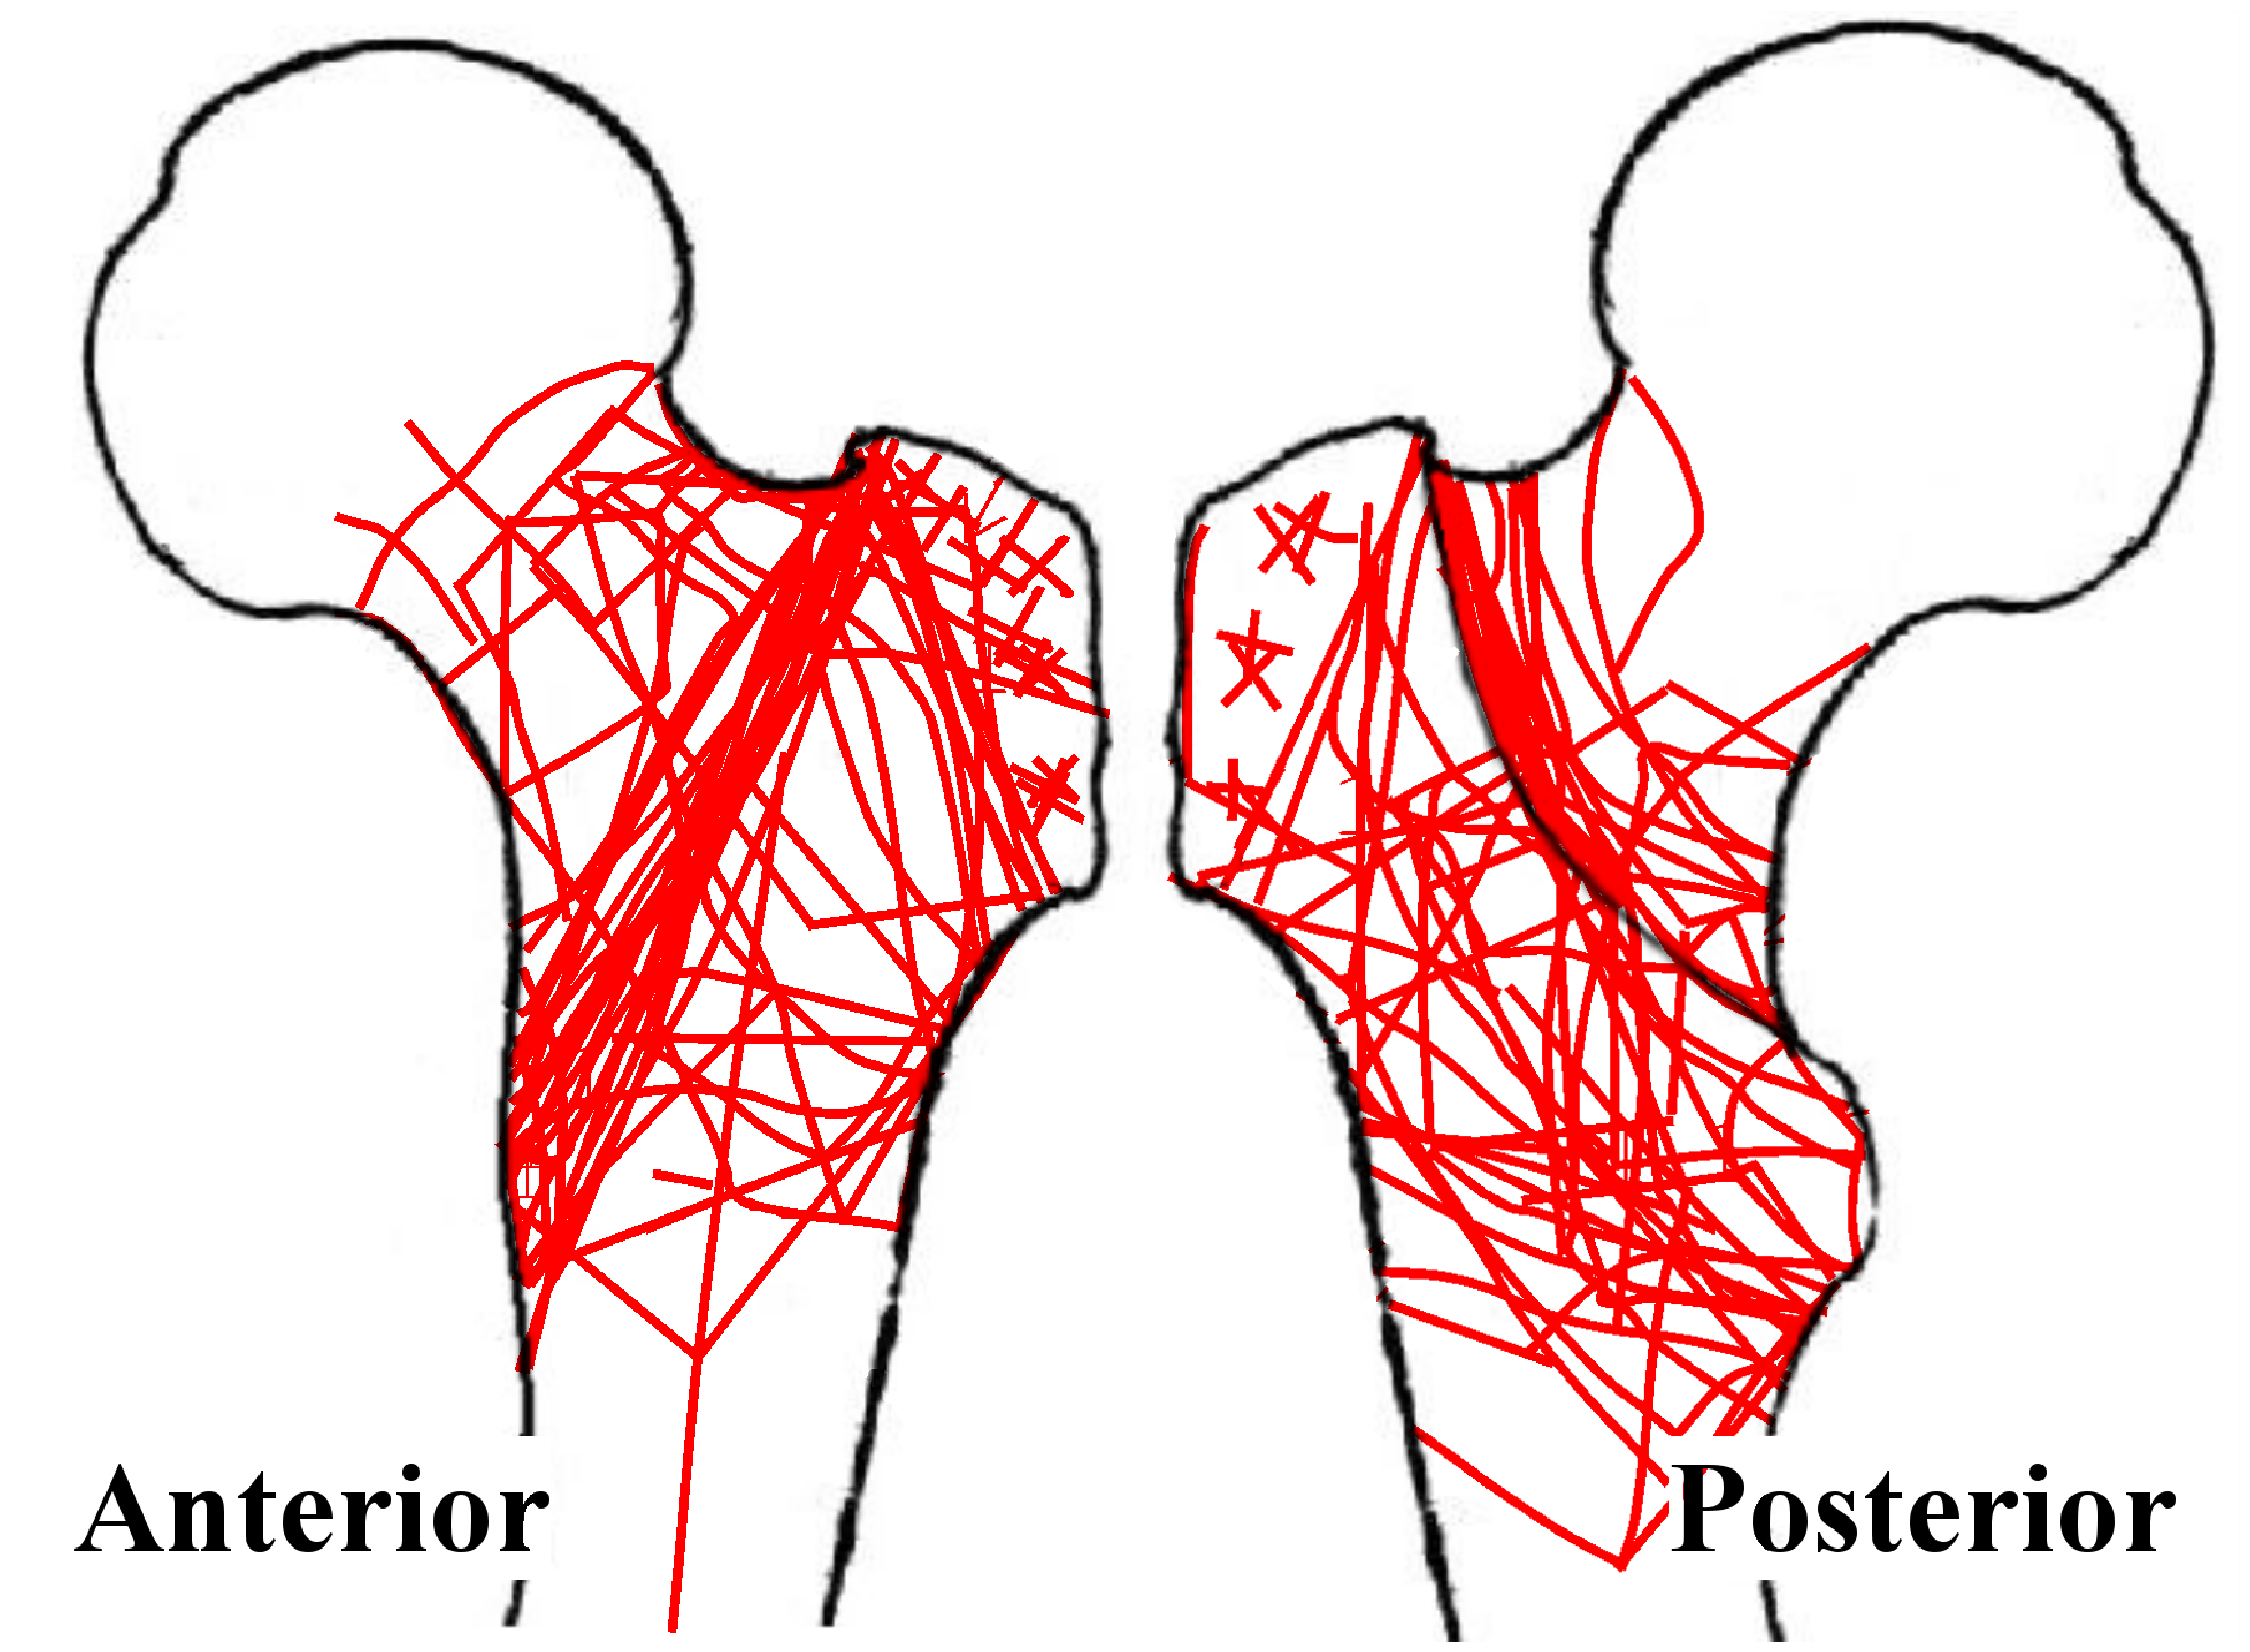
\includegraphics[width=0.7\linewidth]{./fracture/Figures/GilchristFractures.eps}
	\caption[Fall:\acs*{fs} group fracture lines]{\textbf{Fracture lines observed in the fall:\ac{fs} group compiled onto a single femur profile.} Graphic \textcopyright Seth Gilchrist, 2013.}
	\label{fig:GilchristFractures}
\end{figure}

\begin{table}
	\begin{center}
		\caption[Failure locations and fracture types for simulated group]{Initial failure locations and final fracture types for the specimens in the fall:\ac{fs} group} % N = neck, IS = intertrochanteric stable, IU3 = intertrochanteric unstable 3-part, IU4 = intertrochanteric unstable 4-part, ST = subtrochanteric, NFx = no fracture.}
		\label{tab:GilchristFractures}
		\begin{tabular}{|c||>{\centering}p{2em}|>{\centering}p{2em}|>{\centering}p{2em}|>{\centering}p{2em}|>{\centering}p{2em}|>{\centering}p{2em}|c|}
			\hline 
			\multirow{2}{*}{Specimen}	& \multicolumn{6}{c|}{Fracture Types}	 & \multirow{2}{*}{\lbCell{Initial Failure \\ Location}} \\ \cline{2-7}
		 & \ac{neck} & \ac{is} & \ac{iu3} & \ac{iu4} & \ac{st} & \ac{nfx} & \\ \hline
			\hline 1 		& \checkmark &  & & \checkmark & & 	& Intertrochanteric \\
			
			\hline 2 		&  & \checkmark &  &  &  & 			& Intertrochanteric \\
			
			\hline 3 		&  &  &  &  &  & \checkmark			& Superior Neck		\\
			
			\hline 4 		& \checkmark &  & \checkmark &  & \checkmark & 	& Trochanteric 		\\ 
			
			\hline 5 		&  &  & \checkmark &  &  & 			& Intertrochanteric \\ 
			
			\hline 6 		& \checkmark &  & \checkmark &  &  &  	& Trochanteric		\\ 
			
			\hline 7 		&  &  & \checkmark &  &  & 			& Trochanteric		\\ 
			
			\hline 8 		& \checkmark &  &  &  &  & 			& Superior Neck		\\ 
			
			\hline 9 		&  &  &  & \checkmark &  & 			& Trochanteric		\\ 
			
			\hline 10 		& \checkmark &  &  & \checkmark &  & & Trochanteric		\\
			
			\hline 11 		& \checkmark &  &  &  &  &			& Superior Neck		\\ 
			
			\hline 12 		&  &  & \checkmark &  &  &  		& Trochanteric		\\ 
			
			\hline 13 		&  &  & \checkmark &  &  & 			& Intertrochanteric	\\ 
			
			\hline 14 		&  &  &  &  &  & \checkmark			& Trochanteric		\\ 
			
			\hline 15 		&  & \checkmark &  &  &  & 			& Intertrochanteric	\\ 
			
			\hline 16 		& \checkmark &  & \checkmark &  &  & & Intertrochanteric	\\ 
			
			\hline 17 		&  & \checkmark &  &  &  & 			& Intertrochanteric	\\ 
			
			\hline 18 		& \checkmark &  & \checkmark &  &  & & Intertrochanteric	\\ 
			
			\hline 19 		&  & \checkmark &  &  &  & 			& Trochanteric		\\ 
			
			\hline 20 		&  & \checkmark &  &  &  &  		& Intertrochanteric	\\ 
			
			\hline 21		&  &  & \checkmark &  &  &  		& Trochanteric		\\ 

			\hline 22 		& \checkmark &  &  &  & \checkmark & 			& Superior Neck 	\\ 
			
			\hline 23 		& \checkmark & \checkmark &  &  &  &  			& Trochanteric 		\\ 

			\hline 24 		& \checkmark &  &  &  &  &  		& Not Available		\\ 
			
			\hline 
		\end{tabular} 
	\end{center}
\end{table}

\begin{figure}
	\centering
	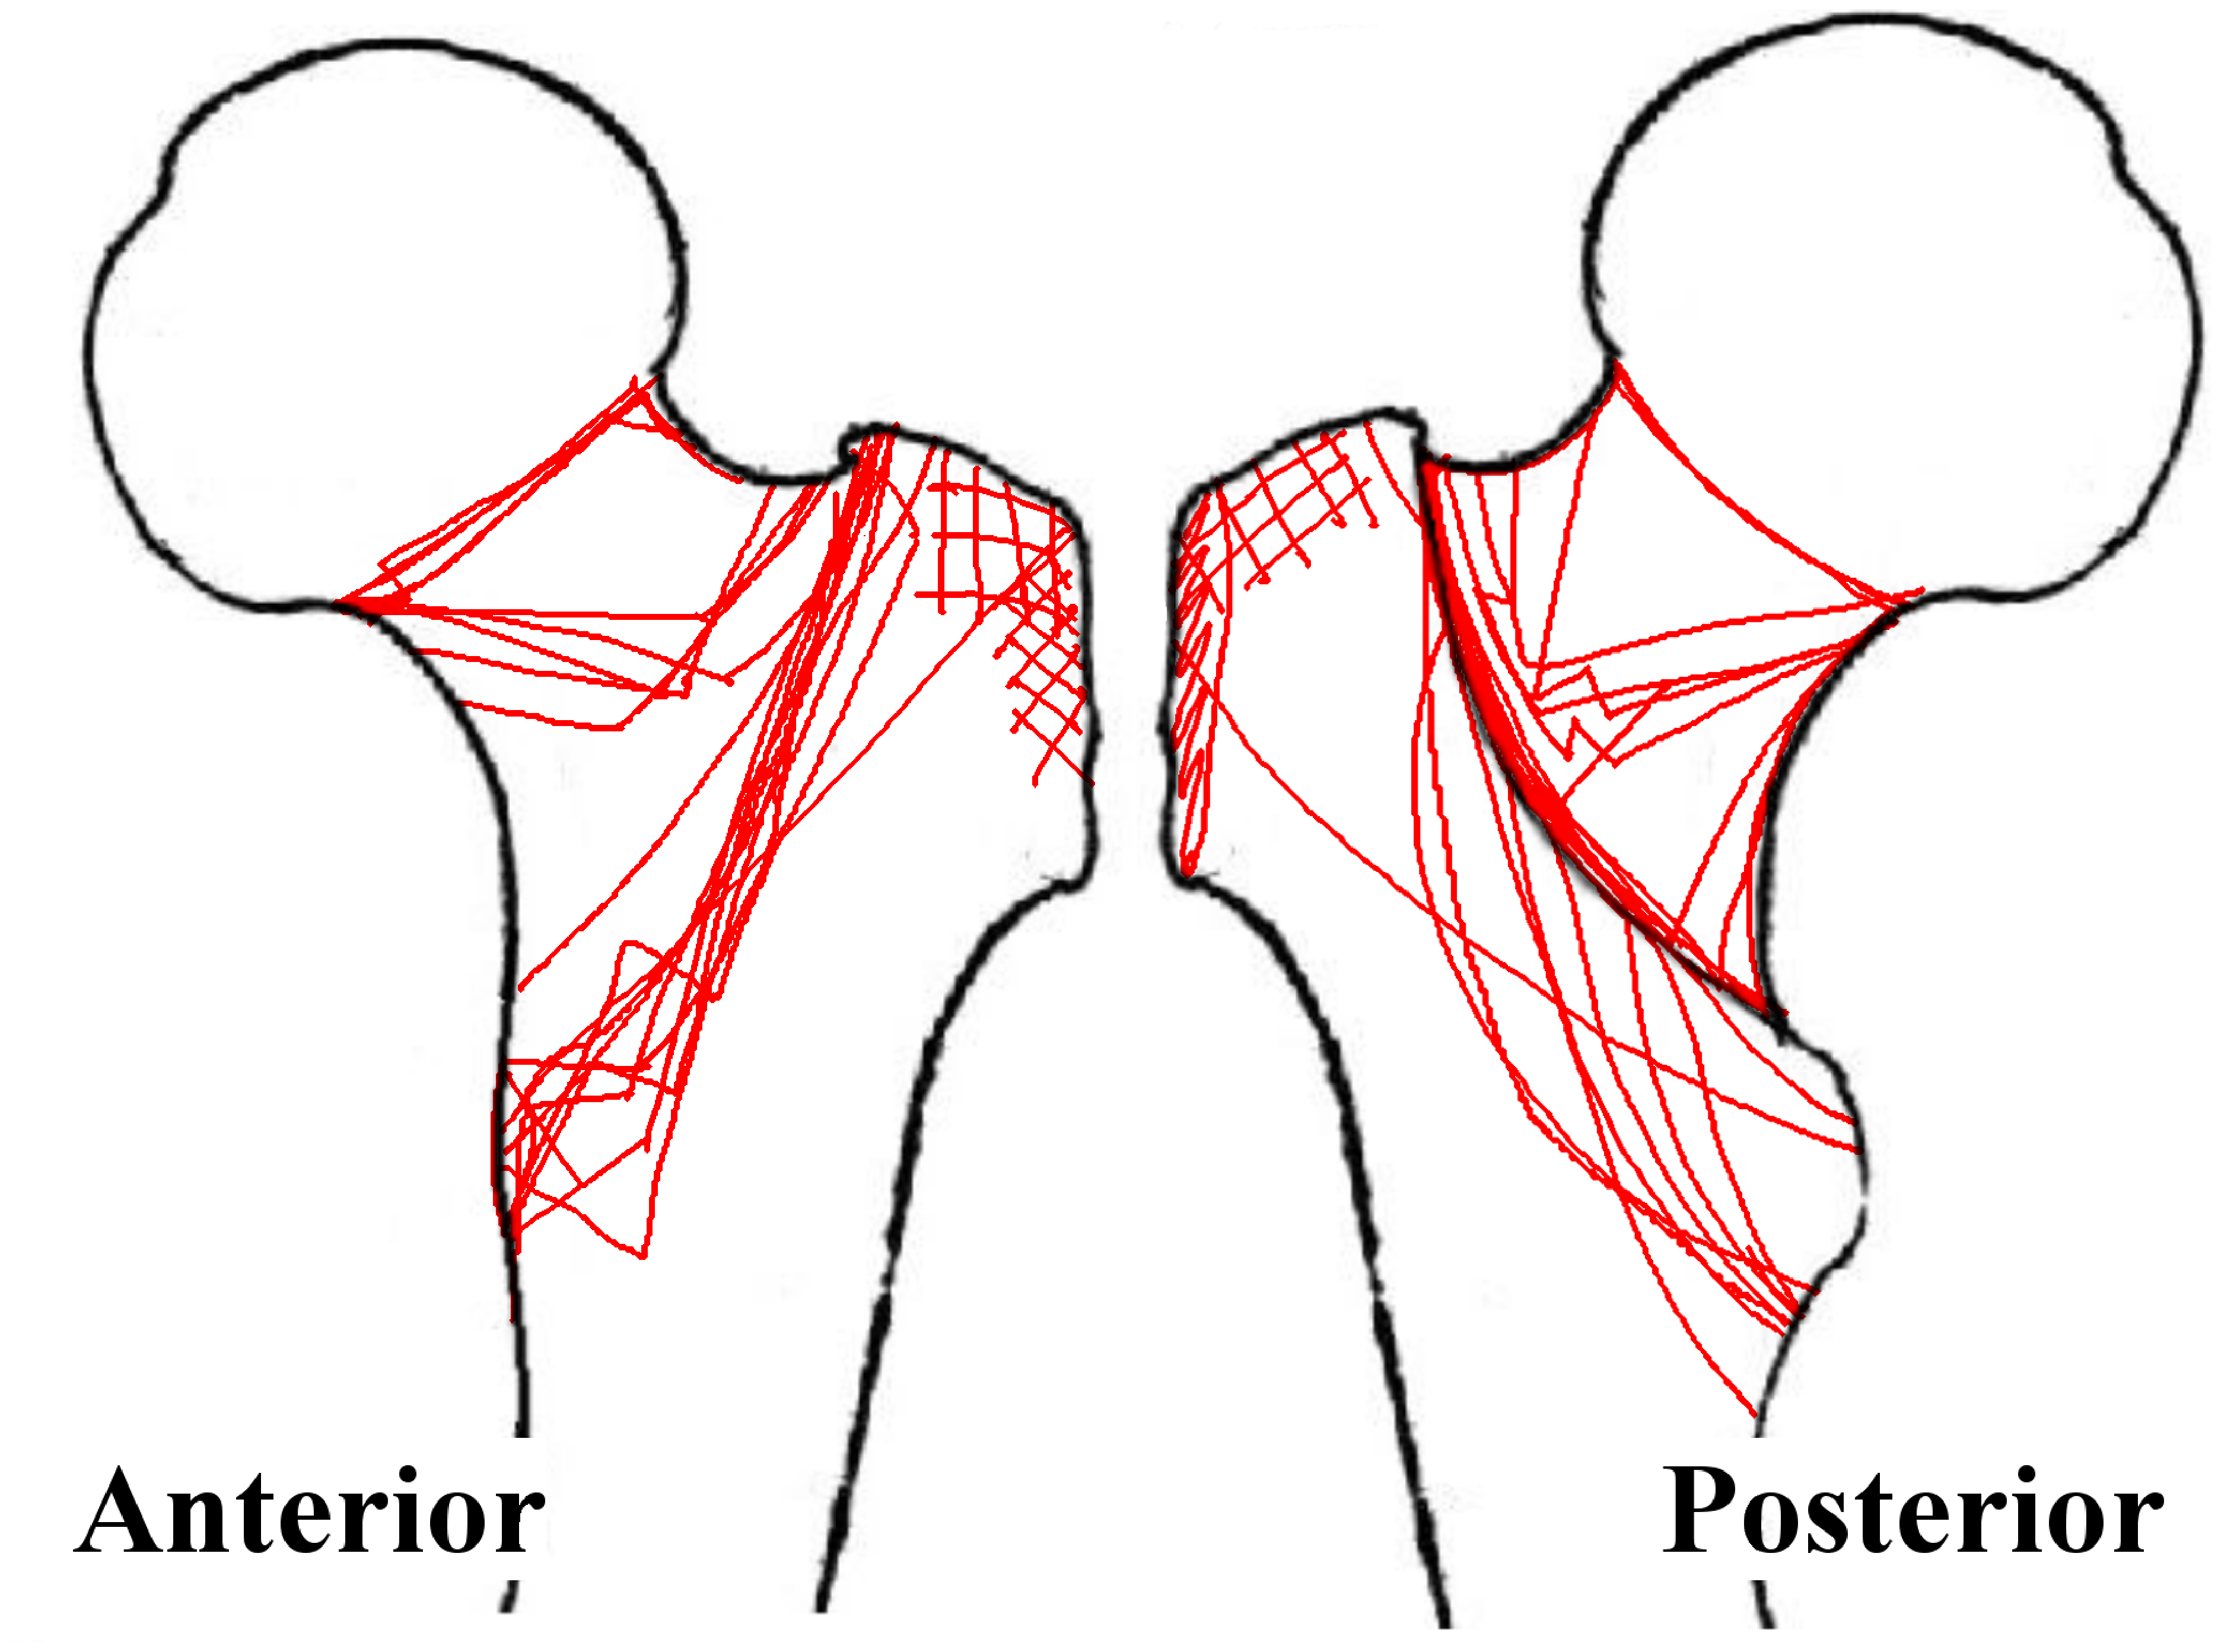
\includegraphics[width=0.7\linewidth]{./fracture/Figures/NishiyamaFractures.eps}
	\caption[Slow group fracture lines]{\textbf{Fracture lines observed in the slow group compiled onto a single femur profile.} Graphic \textcopyright Seth Gichrist, 2013.}
	\label{fig:NishiyamaFractures}
\end{figure}

\begin{table}
	\begin{center}
		\caption[Failure locations and fracture types for slow group]{Initial failure locations and final fracture types for the specimens slow group} % N = neck, IS = intertrochanteric stable, IU3 = intertrochanteric unstable 3-part, IU4 = intertrochanteric unstable 4-part, ST = subtrochanteric, NFx = no fracture. }
		\label{tab:NishiyamaFractures}
		\begin{tabular}{|c||>{\centering}p{2em}|>{\centering}p{2em}|>{\centering}p{2em}|>{\centering}p{2em}|>{\centering}p{2em}|>{\centering}p{2em}|c|}
			\hline 
			\multirow{2}{*}{Specimen}	& \multicolumn{6}{c|}{Fracture Types}	 & \multirow{2}{*}{\lbCell{Initial Failure \\ Location}} \\ \cline{2-7}
			 & \ac{neck} & \ac{is} & \ac{iu3} & \ac{iu4} & \ac{st} & \ac{nfx} & \\ \hline
			
			\hline 1		&  &  & \checkmark &  &  & 			& Intertrochanteric	\\ 
			
			\hline 2		&  &  & \checkmark &  & &			& Intertrochanteric	\\ 
			
			\hline 3		&  & \checkmark &  &  &  & 			& Intertrochanteric	\\ 
			
			\hline 4		& \checkmark &  &  &  &  &  		& Superior Neck		\\ 
			
			\hline 5		&  & \checkmark &  &  &  &  		& Unknown		\\ 
			
			\hline 6		&  & \checkmark &  &  &  &  		& Intertrochanteric	\\ 
			
			\hline 7		& \checkmark &  &  &  &  & 			& Superior Neck		\\ 
			
			\hline 8		& \checkmark &  &  &  &  & 			& Superior Neck		\\ 
			
			\hline 9		&  & \checkmark &  &  &  &  		& Intertrochanteric	\\ 
			
			\hline 10		& \checkmark &  &  &  &  & 			& Superior Neck		\\ 
			
			\hline 11		&  & \checkmark &  &  &  &  		& Unknown		\\ 
			
			\hline 12		& \checkmark &  &  &  &  & 			& Superior Neck		\\ 
			
			\hline 13		& \checkmark &  &  &  &  & 			& Intertrochanteric	\\ 
			
			\hline 14		& \checkmark &  &  &  &  & 			& Unknown		\\ 
			
			\hline 15		&  & \checkmark &  &  &  &  		& Intertrochanteric	\\ 
			
			\hline 16		& \checkmark &  &  &  &  & 			& Superior Neck		\\ 
			
			\hline 17		& \checkmark &  &  &  &  & 			& Inferior Neck		\\ 
			
			\hline 18		&  & \checkmark &  &  &  &  		& Unknown		\\ 
			
			\hline 19		&  & \checkmark &  &  &  &  		& Superior Neck		\\ 
			
			\hline 20		&  & \checkmark &  &  &  &  		& Intertrochanteric	\\ 
			
			\hline 
		\end{tabular}
	\end{center}
\end{table}

\begin{table}
\caption[Initial failure and final fracture locations]{Initial failure locations and final fracture locations in each group}
\label{tab:initial_final_fast}
\begin{subtable}{0.45\textwidth}
\centering
\caption{Fall:\ac{fs} group}
\begin{tabular}{r c c c}
 & & \multicolumn{2}{c}{Initial} \\
 & & \multicolumn{1}{|c|}{Neck} & \multicolumn{1}{c|}{Other} \\
 \cmidrule{2-4}
 \multirow{2}{*}{\rotatebox{90}{Final}} & \multicolumn{1}{c|}{Neck} & \multicolumn{1}{c|}{3} & \multicolumn{1}{c|}{7} \\
 \cmidrule{2-4}
  & \multicolumn{1}{c|}{Other} & \multicolumn{1}{c|}{1} & \multicolumn{1}{c|}{12}\\
 \cmidrule{2-4}
\end{tabular}
\end{subtable}
\begin{subtable}{0.45\textwidth}
\centering
\caption{Slow group}
\begin{tabular}{r c c c}
 & & \multicolumn{2}{c}{Initial} \\
 & & \multicolumn{1}{|c|}{Neck} & \multicolumn{1}{c|}{Other} \\
 \cmidrule{2-4}
 \multirow{2}{*}{\rotatebox{90}{Final}} & \multicolumn{1}{c|}{Neck} & \multicolumn{1}{c|}{7} & \multicolumn{1}{c|}{1} \\
 \cmidrule{2-4}
  & \multicolumn{1}{c|}{Other} & \multicolumn{1}{c|}{1} & \multicolumn{1}{c|}{7}\\
 \cmidrule{2-4}
\end{tabular}
\end{subtable}
\end{table}

The comparison of the surface strains in the fall:\ac{QS} and fall:\ac{fs} tests at the same load, and location showed that there were significant differences between the test conditions ($p < 0.01$, Fig.~\ref{fig:StrainDiffs}).
When all fall group data were pooled, the fall:\ac{QS} strain was 221~\ac{micro-eps} higher than the fall:\ac{fs} strain ($p = 0.45$, 95\%~\acs{ci}~=~(921,~-477)), which was 6.9\% of the average quasi-static strain of -3205~\ac{micro-eps}.

Comparison of the strain fields showed that they were typically correlated, but often exhibited an offset in the measured strain (Fig.~\ref{fig:StrainDiffs}).
The average \acs{rms} error in the surface matching was 5.3*10\textsuperscript{-11}~\ac{m}, indicating that the majority of the 50,000+ points in each surface were nearly coincident after the registration.
Some of the strain comparisons displayed ``branches" on the strain-strain plots (specimens 15, 24, 25 and 26), which were indicative of a redistribution of the strain field.
To illustrate this, specimen 24, which showed two branches in the strain-strain plot (Fig.~\ref{fig:StrainDiffs}), was seen to have two locations where the strains were different, one on the lateral neck and the other in the sub-capital region (Fig.~\ref{fig:H1380R_FemurOverlay}).
The locations of the differences in strain were qualitatively examined in specimens 15, 24, 25 and 26 and the redistributions did not seem systematic, rather they appeared random.

\section{Discussion}
This experiment studied the strain distributions, failure locations and fracture patterns between quasi-static, fixed displacement rate and impact fall simulation loading protocols.
The failure study showed that final fracture patterns were significantly different between the two groups, even though the initial failure locations were not.
This leads us to reject the null hypotheses that fracture types are the same between quasi-static and fall simulation testing, and accept the null hypothesis that initial failure locations are the same in both testing methods.
The strain between the two sub-failure tests conditions were significantly different on a point by point basis, but when pooled together there was no significant trend.
Therefore, testing of the hypothesis that there would be a significant difference in strain lead to two solutions, firstly, we reject the null hypothesis that there would be no difference in strain on any given proximal femur between the two testing methods, however, we accept the null hypothesis that there is no significant difference between the testing methods on a population level.

\afterpage{
\begin{landscape}
\begin{figure}
	\centering
	\includegraphics[width=\linewidth]{./fracture/Figures/StrainDiffs}
	\caption[Strain differences for specimens in the simulated group]{\textbf{Strain-strain plots comparing minimum compressive strain between the fall:\ac{QS} and fall:\ac{fs} groups.
	Each point in each plot is at the same location and load, and the \textit{p}-values are the results of a paired t-tests on all points in the point cloud.} Graphic \textcopyright Seth Gilchrist, 2013.}
	\label{fig:StrainDiffs}
\end{figure}
\end{landscape}
} % afterpage

\begin{figure}
	\centering
	\includegraphics[width=0.9\linewidth]{./fracture/Figures/H1380R_FemurOverlay}
	\caption[Strain differences overlaid on an example bone]{\textbf{Fall:\ac{QS} minus fall:\ac{fs} minimum principal strains at the same load overlaid on the specimen.
	In this case, the fall:\ac{fs} tests had higher strains in the lateral neck and lower strains along the subcapital line.
	The average strain difference for this specimen was 39~\ac{micro-eps}, with a range of [-770, 470]~\ac{micro-eps}.} Graphic \textcopyright Seth Gilchrist, 2013.}
	\label{fig:H1380R_FemurOverlay}
\end{figure}

\begin{table}
	\centering
	\caption{Published fracture locations for laboratory experiments}
	\label{tab:labFx}
	\begin{tabular}{p{8cm} >{\centering}p{2cm} c}
		\toprule
		Author                                  &     Neck     & Trochanteric \\ \midrule
		\citet{backman_proximal_1957}           &      36      &     117      \\
		\citet{lotz_use_1990}                   &      6       &      6       \\
		\citet{weber_proximal_1992}             &      8       &      7       \\
		\citet{courtney_effects_1994} (Elderly) &      5       &      4       \\
		\citet{courtney_effects_1994} (Young)   &      6       &      3       \\
		\citet{pinilla_impact_1996}             &      8       &      3       \\
		\citet{keyak_prediction_2001}           &      4       &      10      \\
		\citet{lochmuller_mechanical_2002}      &      54      &      40      \\
		\textbf{Totals}                         &  \textbf{127} &  \textbf{190} \\ \bottomrule
	\end{tabular} 
\end{table}

\begin{table}
	\centering
	\caption{Published fractures locations for clinical studies}
	\label{tab:clinicalFx}
	\begin{tabular}{p{8cm} >{\centering}p{2cm} c}
		\toprule
		Author                                &      Neck      &  Trochanteric  \\ \midrule
		\citet{michelson_epidemiology_1995}   &       63       &       83       \\
		\citet{lyritis_epidemiology_1996}     &      791       &      995       \\
		\citet{sirois_burden_2009}            &      783       &      1584      \\
		\citet{lefaivre_changes_2011}         &     22313      &     19677      \\			
		\citet{poole_cortical_2012}           &       36       &       39       \\
		\textbf{Totals}                       & \textbf{23986} & \textbf{22378} \\ \bottomrule
	\end{tabular}
\end{table}

Comparison of the fracture outcomes of the current experiments to those published in the clinical literature is complicated by the lack of post fracture x-rays in the current tests.
Clinical fractures are diagnosed and classified using radiological examination, however, in the fall group, the fall simulator often destroyed the greater and lesser trochanter of the specimens post fracture, making radiological examination impossible.
That said, classification as either intra- or extracapsular was possible from fragment analysis and video observation and the current results are in-line with previous tests and clinical observations (Tables~\ref{tab:labFx} and~\ref{tab:clinicalFx}).
The fall:\ac{fs} fractures were split 50/50 between intra- and extracapsular fractures, while the slow group showed a slight tendency toward extracapular fractures.
Both methods gave distributions of fracture types that are representative of what has been observed in the clinical literature.

Examination of the strain values on the surface of the specimens at the same compressive load while being tested with the two protocols showed that average strain over the analysis regions was not statistically different between the two testing protocols, however, no single specimen had the same strain.
These results seem contradictory, however, they are indicative of a random variation in surface strain due to the change in loading protocol.
A cohort of specimens loaded quasi-statically will show, on average, the same strain as those loaded in the impact fall simulator, however, each individual specimen will have a different response in the two tests.
This result has important implications for study design.
If a case-series study is examining the change in strain due to an intervention in which two sufficiently sized cohorts of specimens are treated in two different ways, quasi-static, constant displacement rate simulations will be sufficient to study the effects of the intervention.
However, if a study is examining changes in a specimen specific manner, \ac{eg}, trying to identify the correct intervention to decrease surface strains in a particular specimen, then impact fall simulation is warranted.

It should be noted that alignment errors in the registration process could have led to differences being detected between specimens that were not real.
If the \ac{dic}-measured surfaces were not perfectly aligned, the strain gradients on the surface could manifest as a reconfiguration of strain in the strain-strain plots.
However, each comparison in this study was individually inspected for two features:
\begin{inparaenum}[i\upshape)]
\item \label{item:dic_surf} surface size, extent and off-plane features, and
\item location of strain differences.
\end{inparaenum}
The first item was important for ensuring a reliable registration.
Surfaces that were either flat or described only a portion of a cylindrical surface were eliminated from the comparisons.
Features that were considered sufficient for inclusion of a surface were extension of the surface onto the femoral head or trochanter in a way that provided an out of plane, or off-cylindrical axis registration target.
The second item was a post-processing analysis aimed at identifying if the branches seen in the strain-strain plots were in close physical proximity.
If the locations of strain difference were physically near each other, the surfaces were re-evaluated in terms of (\ref{item:dic_surf}) and either eliminated if the surface was insufficient for accurate alignment, modified if an identifiable feature was driving a misalignment, or accepted if the registration was driven by a sufficiently complex surface.


A few specimens showed redistributions of strain on the anterior superior femoral neck that were, in some cases, quite large.
This reasons for this are unknown, but could be related to failures of cancellous bone below the surface early in the loading which are not visible in the current tests.
Failure within the structure could cause the load path to be altered, which could manifest as a change in pattern and magnitude on the surface.

To our knowledge, this study is the first of its kind to compare the failure locations, and fracture patterns in two populations tested at considerable extremes of loading protocols, as well as to examine the strain fields of individual specimens loaded to sub-failure using different protocols.
Like all \textit{ex-vivo} fracture experiments, this study has some limitations that we did our best to mitigate, but must be considered during interpretation.
First of all, the small number of specimens reduces the power to identify differences between the fall and slow groups.
That said, most of the comparisons between the two methods resulted in statistical results that were sufficiently powerful that more specimens would not have been required.
Once exception to this may be the initial failure location.
It was not seen to be different, but the \textit{p}-value of 0.13 could be considered a trend worth further investigation.
Secondly, the impact testing protocol resulted in the destruction of the specimens and consequently post fracture \ac{a-p} x-rays were not possible.
Since clinical fracture evaluation is carried out using \ac{a-p} x-rays, the results of this work are not directly comparable to clinical outcomes.
However, the classification into intra- and extracapsular fractures should be comparable due to the distinctly different locations of these portions of the proximal femur.
Additionally, some of the fractures were such that they may not have been observed using a-p x-ray examination.
These fractures were hairline fractures along the superior femoral neck, in the coronal plane and may represent failures not yet documented in the clinical literature.
Finally, the strain mapping was carried out only on the superior-anterior surface of the femoral neck, which may not be representative of the proximal femur as a whole.
This fact limits the applicability of the no difference when pooling data result, but it does not limit the applicability of the observations on individual specimens where we can say that in the critical location of the anterior-superior neck, the response is different between the two loading methods.
Additionally, the density of the strain data are much higher than previous tests utilizing strain gauges and thus provides a rich dataset for statistical analysis.

Overall, this work indicates that more biofidelic replication of the fall and fracture scenario may benefit the examination of hip fracture progression.
The changes in final fracture types and the redistribution of strain in some specimens may be indicative of internal mechanics that have heretofore gone unobserved.
The examination of fracture patterns in two similar populations tested in two very different scenarios allowed us to understand how loading mechanism affects failure through rate-dependent failure changes.
Our interpretation of the results lead us to recommend that experiments in which single specimens are treated in different manners with the goal of influencing strain development or fracture behaviour use fall simulation to test outcomes.
However, if general changes in a cohort of specimens are to be observed, quasi-static testing at constant displacement rate, or impact fall simulation can be used.
We believe that future finite element research should concentrate on incorporating strain-rate dependency in material properties, and create specimen-specific models whose fracture predictions are validated using applicable loading rates.
These models could be used to identify the critical load path in a fall to the side, and investigate the effects of changing this load path due to local failures within the cancellous and cortical bone.
This technique could help understand the phenomena of how an initial failure in the trochanter can lead to fracture of the neck in fall simulation.
Ultimately, we aim to understand how forces are transferred in a compromised femur, potentially giving us the tools to develop intervention and screening technologies that would reduce the burden of this devastating condition.

\chapter{Communication between mechanical and \acl*{fe} modelling}
\label{ch:modelling}
Mechanical and \acf{fe} modelling are closely linked.
Much of the work done in \ac{fe} modelling is a continuation or examination of phenomena observed in experimental modelling, and many experiments are conducted in support of \ac{fe} model validation.
A considerable portion of the work in this thesis was done in conjunction with the \ac{fe} modelling team under the supervision of Dr.\ Ben Helgason at ETH, Z\"{u}rich, Switzerland.
There was significant effort expended to ensure that the \ac{fe} modelling group had all the data required to create models that could be readily compared to the experiments performed.
This chapter gives a brief description of the data flow between the two modelling methods and efforts made on the experimental side to facilitate that flow.
Informally, we have dubbed this the \textit{data pipeline}.
I hope that future \ac{fe}-experiment collaborations can take advantage of my experience in this regard.

\section{Documentation from start to finish}
\label{sec:modelling_document}
The most critical aspect in creating an experiment that can be used for \ac{fe} validation is documentation and transparency.
From apparatus, to data and analysis routines, all aspects of the experiment must be fully described and accessible to the modelling community (Figure~\ref{fig:modelling_Dataflow}).

Details of experimental apparatus are useful in defining \acfp{bc} of \ac{fe} models.
The level of detail required in an \ac{fe} model may begin modestly, but as the model is refined researchers may need to integrate very high levels of detail in some aspects of the setup.
Since it cannot be easily anticipated where certain phenomena originate, experimental modellers must make an almost arbitrary level of detail available to the \ac{fe} modellers.
The purpose of an \ac{fe} model is frequently to examine aspect of the experiment that are difficult to explain based on current knowledge, which means that current knowledge should be used cautiously in determining what to include in a model.
As computational power increases, \ac{fe} researchers are including more apparatus in their models in an effort to close the gap between computational and experimental models; details provided by the engineers who designed the experimental apparatus can help the two models converge.

Computer code and analysis routines is another area where concerted effort to organize and communicate can pay off.
\ac{fe} researchers want data packed in a manner that makes data manipulation and extraction easy to automate.
Additionally, code annotation and inclusion of details like units used in a given portion of the analysis can be invaluable to an \ac{fe} modeller who is working remotely from the experimental researchers.
This kind of annotation and documentation of code is time consuming and can be challenging.
Experimentalists often use one-off custom code, with the routines designed to evaluate specific variables of concern for a given test.
Each researcher typically develops their own code, based on their own needs, that they understand well and rarely pass on to future experimentalists.
Computational researchers are used to developing and documenting code with the intent of passing it to the next researcher.
Indeed, very little progress would be made in the field if each \ac{fe} researcher had to start from scratch.
Additionally, in the computational world there is an understanding that no code is perfect, as evidenced by the continual releases of new versions of old software.
Experimentalists can be overtly aware of limitations, coding discrepancies and the nuances of running their software, which can make them reluctant to open-source it for fear of criticism~\citep{barnes_publish_2010}.
To address the latter fear, documentation must be an integral part of the analysis code development process, with the expectation that it will be released, along with the data, to another research group.
This was handled in the current work by developing a series of analysis classes that were portable and self contained (\S\ref{sec:code_dt_ins_analysis}).
Each class object contained the raw data, the final data, filtering and interpolation routines that yielded the final data, and routines to analyse and extract meaningful data, as well as variables concerned with those analyses.
This transparency and documentation allowed sending the data to researchers who were unfamiliar with the tests, and allowing them to access the full analysis, as well as documentation (including information like units) for each test and specimen.

\begin{figure}
\centering
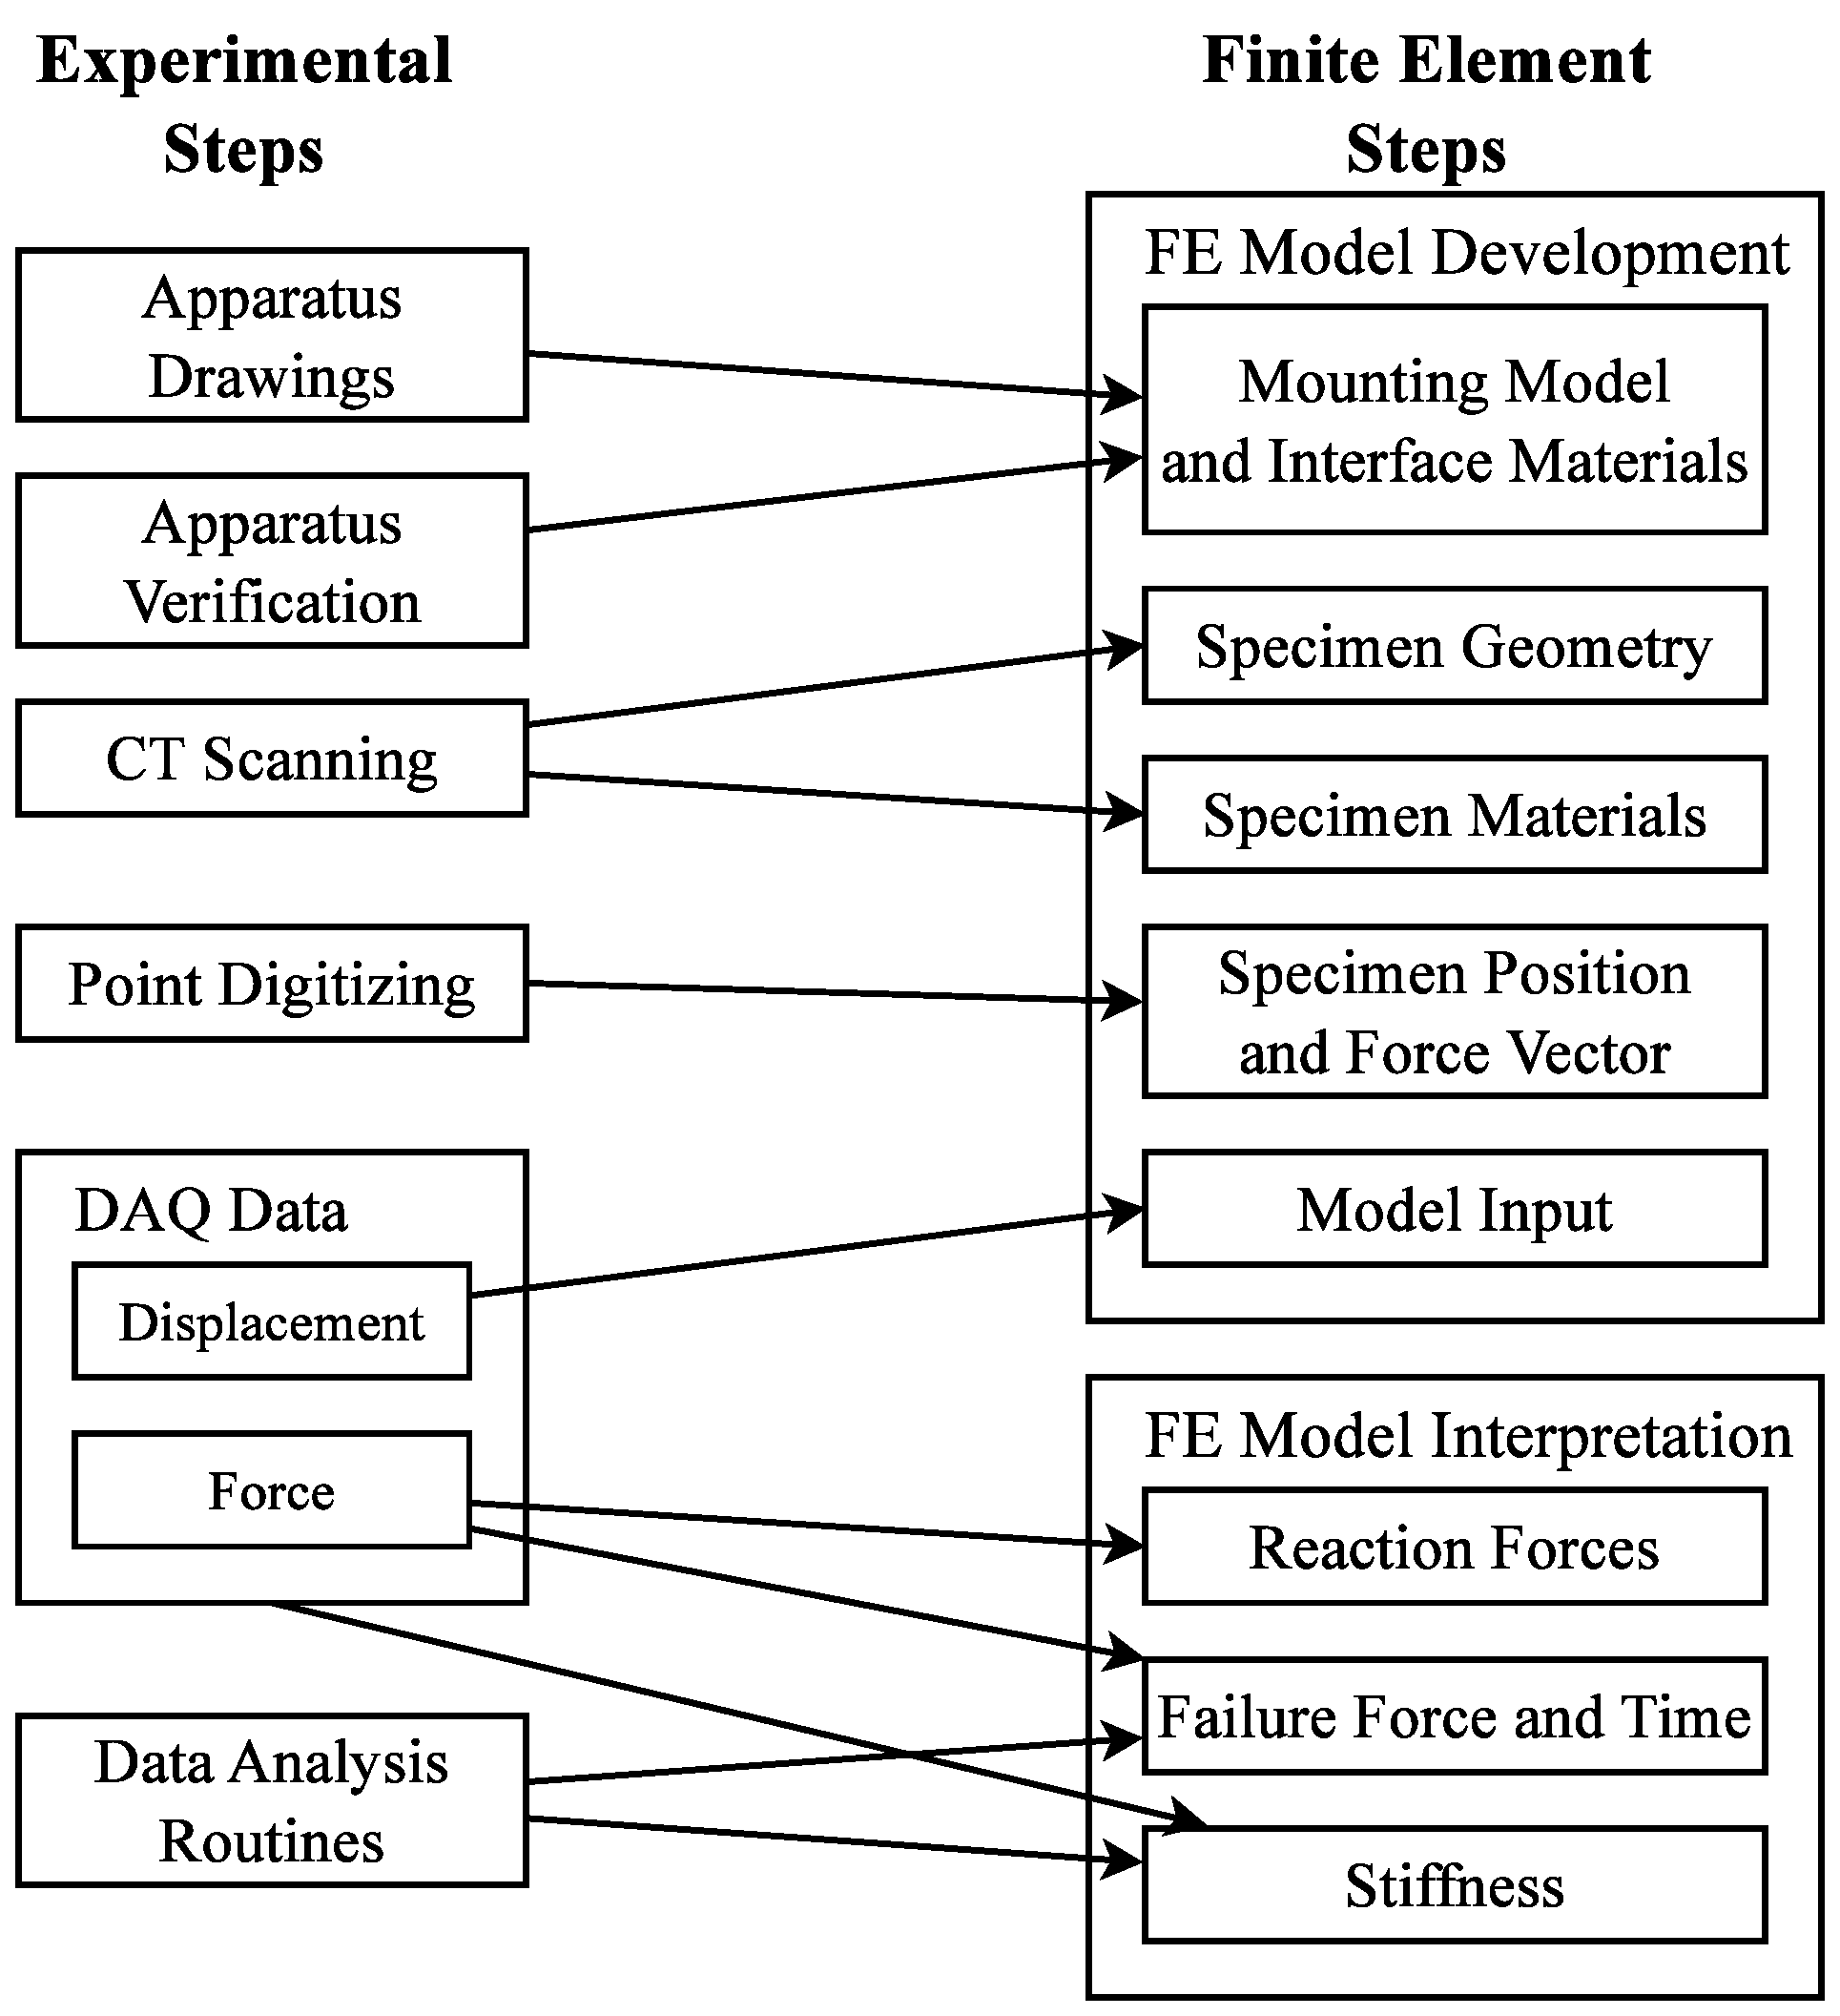
\includegraphics[height=\textwidth]{./testing_fe_modelling/figures/Dataflow}
\caption[Experimental and \acs*{fe} data flow]{\textbf{Flow of data between experimental and \ac{fe} modelling techniques. Documentation from the beginning is key and access to analysis routines is important for comparing data on an even footing.} Graphic \copyright Seth Gilchrist, 2013.}
\label{fig:modelling_Dataflow}
\end{figure}

\section{Additional data for \acs*{fe} modelling}
\label{sec:modelling_additional}
As mentioned in the previous section, the origins of phenomena observed in an experiment are often difficult to predict.
One potential source of obfuscation is poorly or incorrectly applied \acp{bc}.
This can be addressed by careful recording of experimental setup using technologies like \ac{ct}, surface digitization and landmark point digitization.
The majority of experimental models do not need for \ac{ct} imaging and surface topology of specimens.
\acs{a-p} radiographs and \ac{dxa} images are used by researchers to give a clinical context to the specimens being tested.
When working with \ac{fe} models, detailed geometric, densitometric and orientation data are needed, requiring collection of \ac{ct} images, as well as bone and test equipment landmarks.

Once the drawings of the apparatus, and geometry and density of the bones are obtained, an \ac{fe} model can be constructed and appropriate fixed boundary conditions applied.
The effector of an \ac{fe} model is typically a displacement or force \acl{bc}, the alignment of which is critical to the output of the model.
To align the force or displacement application in the computational model, the orientation of the bone during the actual experiment must be obtained.
This was done by collecting the (\textit{x,y,z}) coordinates of points on the surface of the bone and loading apparatus using an Optotrak (Certus, NDI, Ontario, Canada) with a digitization wand (Figure~\ref{fig:digitizing}).
Points were collected on each part of the specimen and apparatus and saved in a text file.
Approximately 30 points were taken on the femoral head, 30 on the femoral neck, 30 on the trochanter, 20 on the shaft, 20 on interface between each \ac{pmma} cup and the bone, 4 on the bottom platen, 6 on each side of the pivot, 8 on the impact hammer and finally 2 on the strain gauge.
The organization of the points was recorded in a log sheet (given in full in~\S\ref{sec:support_logsheets}) which was provided to the \ac{fe} modellers for reference.

\begin{figure}
\centering
\includegraphics[width=\linewidth]{./testing_fe_modelling/figures/digitizing}
\caption[Digitizing points on the experimental apparatus]{\textbf{In this image, taken from a video of the setup procedure, the Optotrak digitizing wand is being used to digitize the location of the pivot at the distal end of the femoral shaft.} Image \copyright Seth Gilchrist, 2013.}
\label{fig:digitizing}
\end{figure}

\section{Data portability and transparency}
\label{sec:modelling_portable}
Data from the experiment are used to drive the \ac{fe} model and validate the output.
The models of the current tests, created by Oscar Ariza in Dr. Ben Helgason's facilities, used a velocity derived from the displacement data as the affecting \ac{bc}.
Other models may use a force \ac{bc}, but in any case, the modellers need to have access to the data and any filtering or post processing that was conducted.

The sources of the data, while important to a mechanical modeller, are of less importance to the computational community.
Instead, computational modellers are more concerned with consistency in data preparation and organization, allowing them to automate the process of extracting needed \acp{bc}.
For example, in the tests conducted in this thesis, displacement in the materials testing machine was recorded by a \ac{daq} from a voltage signal emitted by the materials testing machine, but in the fall simulator displacement was extracted from optical measurements of the trochanter and impact hammer.
Computational modellers would like the data to be accessed in a similar way, regardless of the fact that is was collected using different techniques.

Post processing of the data is important to both computational and mechanical modellers.
\ac{fe} modellers obtain force and displacement as outputs of their models, and process those data into stiffnesses or energies which should be directly comparable to the experiment.
This requires knowledge of how the experiment was conducted and how the data was filtered and/or interpolated.

To meet these needs, I developed nine MatLab (2010b, The Mathworks, Natick, MA) classes that contained all raw data, processed data, processing, filtering and analysis functions as members and methods.
This code was fully documented and released under the  \href{http://www.gnu.org/copyleft/gpl.html}{GNU General Public License}, and is included as an appendix to this thesis (\S\ref{sec:code_dt_ins_analysis}).

A major advantage to using classes such as those detailed in \S\ref{sec:code_dt_ins_analysis} is data portability.
Once the ``experiment" class has been given all the information and all the data has been loaded into the respective subclasses, the class object can be saved as a \ac{mat} file and sent to any researcher with the source code for analysis.
The \ac{mat} file contains all the data listed in the previous paragraph and there will be no ambiguity as to how the analysis was performed.

I recommended that data storage and processing be carried out in this way when collaborating with other research groups.
It allows trouble shooting by any researcher familiar with MatLab, removes the need for complex directory systems to contain raw, filtered and processed data and incorporates a built in record of the settings using during processing.

\section{Summary}
\label{sec:modelling_summary}
Validation of \ac{fe} model data using experimental data is critical for ongoing development of computational techniques.
This type of collaboration requires a significant amount of planning and effort on both sides of the problem.
Experimenters must be amenable to the collection of additional data, transparent with data analysis routines and make efforts to store their data in such a way that it can be accessed using automated, batch processes.
Finally, modellers from both teams should meet regularly to critically evaluate both mechanical and \ac{fe} model results.

%% This is the discussion for my UBC PhD Dissertation
%% The parent document is called thesis.tex

\chapter{Discussion and conclusions}
\label{ch:discussion}
\section{Discussion}
\label{sec:discussion_discussion}
Hip fracture research, in the larger sense, has one overall goal: to prevent fractures.
There are a number of different methods for attaining this goal, from life-style interventions to pharmacology, but before any of these can be tried, an individual's risk of fracture must be estimated.
This is where current knowledge is limited.
The majority of hip fractures occur in individuals who would not have been identified using osteoporosis state, which is the current clinical standard for beginning treatment~\citep{stone_bmd_2003}.
On top of that, there is considerable overlap in \acp{bmd} of those who suffer fracture and those who do not~\citep{greenspan_fall_1994}.
From these data, it appears that the current understanding of hip fracture risk based primarily on osteoporosis state and \ac{bmd} does not give sufficient sensitivity to help clinicians reduce fracture rates below their current levels.

One way to increase the screening sensitivity might be through improved identification of physical parameters of the proximal femur that predispose a person to fracture.
In the past, gross geometric properties of the proximal femur have been proposed as supplemental data to osteoporosis state to increase the rates of identification.
In the more recent past, the \ac{frax} score was developed which included medical and family history that has been linked to hip fracture through epidemiological studies.
While gross anatomy of the proximal femur showed promise~\citep{faulkner_simple_1993}, it has never been generally adopted into clinical use, and while there are considerable advantages to the use of the \ac{frax} score (namely, pre-screening without using expensive and potentially dangerous \ac{dxa} scanning~\citep{kanis_frax_2009}), the sensitivity of \ac{frax} is only slightly better than \ac{bmd} and age alone~\citep{van_den_bergh_assessment_2010}, and the specificity of \ac{frax} is highly dependent on the selection of risk bounds~\citep{leslie_fracture_2011}.

The fact that \ac{bmd} accounts for only a portion of those that suffer hip fractures leads us to believe that there may be other important features of the bone which could be used by clinicians to screen for those at risk of a fracture.
A number of studies have indicated that the configuration of the bone itself could be important in determining hip fracture risk.
Cortical bone has been seen to become thinner and trabecularized with age, which could result in a decrease in strength~\citep{crabtree_intracapsular_2001, blain_cortical_2008, mayhew_relation_2005}, and cancellous bone has been seen to have a different morphology in fracture patients than in controls~\cite{manske_cortical_2008, blain_cortical_2008}.
While these data indicate that changes on a bone material level may in part be responsible for fracture susceptibility, the hip fracture research community has not been able to definitely identify what features or configurations are culpable for this change in fracture risk.

Hip fracture modelling, both experimental and computational, has been carried out (or validated) using proximal femurs loaded in materials testing machines (see Table~\ref{tab:model_results} on page~\pageref{tab:model_results} for experimental references).
These machines apply forces by applying a defined velocity at the greater trochanter of the femur.
The selection of the velocity has been shown to be important~\citep{courtney_effects_1994, weber_proximal_1992}, but the actual value that should be used on a specimen specific basis has never been determined.
It is possible that the use of a prescribed displacement rate introduces artefacts that may influence how fractures are initiated, how they propagate, and what features influence them.
If this is indeed the case, the previous data must be evaluated with this in mind and conclusions should be limited to those that are appropriate for the boundary conditions used.
This work was intended to address this final point -- what is the effect of a constant velocity at the greater trochanter and what parameters are influenced by this boundary condition?
Knowledge of which parameters are valid using this boundary condition and what parameters require more biofidelic testing will allow researchers to design and develop experiments and validations to address the specific questions they have.
Additionally, previous research can be reinterpreted and applied in a way that is consistent with the validity of its output variables.

The objective of the research, outlined in~\S\ref{sec:intro_goals}, was to determine if current test methods capture the force-displacement, strain, failure and fracture behaviours of the proximal femur in a fall to the side.
This objective was met by comparing and contrasting three aspects of the proximal femur when the fall was modelled using either constant displacement rate tests or impact fall simulation utilizing a lumped parameter model of the human body.
The aspects that were examined were the
\begin{inparaenum}[(i)]
\item mechanical response as characterized by force and displacement and their integral (energy) and derivative (stiffness) measures;
\item failure response as characterized by maximum force, initial cortical failure location and final fracture pattern; and
\item surface strain.
\end{inparaenum}
Comparisons showed that although the quasi-static, constant displacement rate and impact fall simulations methods were equivalent in many cases, there were also differences for some specific outcome variables.

Quasi-static, constant displacement rate testing used in many previous fracture protocols~\citep{backman_proximal_1957, beckmann_femoroplasty--augmentation_2007, boehm_prediction_2008, courtney_age-related_1995, eckstein_reproducibility_2004, heini_femoroplasty-augmentation_2004, keyak_relationships_2000, lochmuller_mechanical_2002, lotz_use_1990} was hypothesized to be a limitation of these experiments.
While there is evidence that increased displacement rate significantly changes the response of the bone~\citep{courtney_effects_1994, weber_proximal_1992}, to our knowledge no research has been conducted that confirmed if this change is indeed representative of the situation \textit{in-vivo}, or if it is an artefact of the increased (but still constant) displacement rate.

The roots of this uncertainty are in the complexity of bone as a material, and the complex arrangement of the bone in structures like the proximal femur.
It is known that bone is viscoelastic~\citep{carter_compressive_1977, linde_mechanical_1991, mcelhaney_dynamic_1966, crowninshield_response_1974} and there is evidence that the strength of the viscoelastic response is influenced by the presence of bone marrow~\citep{carter_compressive_1977}, however, this relationship is not well understood and anticipating its influence in mechanical testing is difficult.
On top of this, bone properties are anisotropic and in homogeneous~\citep{keaveny_biomechanics_2001}, with values and principal directions that vary continuously within the bone structure~\citep{ascenzi_variation_2011, nazarian_densitometric_2007}.
Knowing how the specific arrangement of the bone in a given specimen will be influenced by a given boundary condition is currently outside the scope of our understanding.
We believe that the best way to address these challenges is to allow the proximal femur freedom to respond to an inertially driven system, similar to a fall.
This allows changes in bone material properties and configurations of bone in the specimen to influence the applied loading profile throughout the failure process.
The bone then determines the force and displacement time history during a test, in a recursive way.

In order to grant these freedoms and answer the research questions in this thesis, we designed an inertially driven impact fall simulator that utilized a lumped parameter model of the human body to reproduce the loading in a fall to the side.
This work was detailed in Chapter~\ref{ch:fall_sim_design}.
The advantage of a fall simulator was that it allowed the bone to respond as a compliant, potentially viscous member in a spring mass system and influence the overall behaviour of the system, in the aforementioned recursive way.
This technique removes artificial loading constraints that may influence the behaviour of the bone leading up to and at fracture.
The method was limited in its ability to model a specimen specific fall because the parameters of the lumped parameter model were fixed, \ac{ie}, the stiffness of the spring, mass of the body and pelvis, and thickness of the tissue over the greater trochanter could not be modified based on knowledge of the donor's age, \ac{bmd} or body habitus.
This limitation could be addressed in future experiments, but the background knowledge required to make informed changes to these parameters currently does not exist.
Additionally, increasing the biofidelity of an experiment will not always increase the power of the experiment to be able to address specific questions.
While a realistic test is desired, if too many variables are adjusted between experiments, the statistical burden of proof can become large and make it difficult to obtain the power required to test a hypothesis in a meaningful way.
It is therefore the responsibility of the researcher to identify the important parameters which drive the outcome under investigation and find realistic values for the other parameters.
We believe that the advantage of reduced constraint of the loading rate on the response of the proximal femur during testing outweighs the potential limitation of a single body being simulated for all specimens.

The question relating to the mechanical response in fall simulator testing \ac{vs} materials testing machine testing was addressed using two tests and is contained in Chapter~\ref{ch:behave_fail} in which one set of femurs was tested in two ways.
This experiment was used to determine if the mechanical behaviours of the proximal femurs were affected by the change in loading technique and hypothesized that there would be changes in stiffness, strain at a point and energy to the failure.
We found that there was no difference in the behaviours of the bones in terms of any of our mechanical metrics.
There were no statistically significant differences in the stiffness, energy or strain on the anterior superior femoral neck if the proximal femur is loaded using quasi-static, constant displacement rate or impact fall simulation.
These data indicate that if the outcomes of experimental testing or \ac{fe} validation are sub-failure force-displacement response, then mechanical testing in a materials testing machine is adequate.

We also compared the results of this test to those of \citet{courtney_effects_1994}, who had identified a strong viscoelastic response when displacement rate at the greater trochanter was changed from 2~to 100~\ac{mm}/\ac{s}.
Our results indicate that the viscoelastic response in the fall simulator was much lower than that observed by \citet{courtney_effects_1994}, even though our average displacement rate was nearly the same as the 100~\ac{mm}/\ac{s} rate used by \citet{courtney_effects_1994}.
This indicates that artificially imposing a high displacement rate at the greater trochanter affects outcomes and may not represent the true behaviour of a specimen in a fall to the side.

The question of whether failure initiation and fracture patterns would change due to loading technique was discussed in Chapter~\ref{ch:fracture}, and addressed by hypothesizing that there would be different initial failure locations and final fracture patterns in the constant displacement rate and impact fall simulation testing.
The initial failure locations were identified using high-speed video of the tests and final fracture types were classified using a clinical classification system by an orthopaedic surgeon.
The initial failure locations were not significantly different between the two tests, but the final fracture types were.
Additionally, in the fall simulation tests, the initial failure locations were not predictive of the final fracture types, whereas in the quasi-static tests they were.

These data, combined with the data in the previous paragraphs indicating that the mechanical behaviours are the same for sub-failure loading, indicate that the sub-failure response of the proximal femur is relatively insensitive to the type of loading used.
However, once failure begins and there is a re-definition of the primary load path, the type of testing used becomes important.
The fact that the initial failure observed using high speed video occurred at nearly the same instant as the force-displacement identified yield indicates that the primary load path, regardless of test method, in the sub-failure regime, is through the cortex of the bone.
Once the failure begins, the primary load path changes and observations of the exterior of the bone are no longer sufficient to determine its course.

The final tests conducted were to determine if the sub-failure strains on the surface of the proximal femur were different between quasi-static, constant displacement rate and impact fall simulation tests and is detailed in Chapter~\ref{ch:fracture}.
The results of these tests indicate that the surface strains were different in any given specimen, but taken as a whole (\ac{ie}, pooling all the data) showed that there was no systematic difference between the two test methods.
The majority of the specimens showed a shift in strain levels, either to higher or lower strain, when tested in fall simulation \ac{vs} quasi-static testing.
In these cases, the patters were similar, but there was a ``DC" offset in magnitude.
Some specimens showed a redistribution of strain on the bone cortex, however the magnitude of the average strain was not significantly higher in one test or the other.

These data seem counter to the \textit{no difference in sub-failure mechanical behaviour} result that was identified in Chapter~\ref{ch:behave_fail}.
The reason for this may be due to lack of statistical power to determine differences in loading behaviours in the previous tests.
Those tests had only five data points per specimen, in contrast to the \ac{dic} strain measurements which obtains full strain fields containing hundreds of data points per specimen.
However, it is important to note that the differences observed in the \ac{dic} results were statistically significant, but may not be physically significant.
The average difference in strain was only about 7\% of the strain value, a result that my be due to variations in the experimental setup.
Regardless, the measured differences are real, and based on our data indicating a diverging behaviour after initial failure, the affect on strain would likely increase at higher loads (remember that the response is being compared at 50\% of the \ac{abmd} predicted failure load).
It is therefore our recommendation that if changes in surface strain in a specimen-specific manner is the desired outcome, fall simulation be employed.
However, if the outcome of a series of tests is a generalized behaviour of strain that will be averaged over a cohort, then either quasi-static, constant displacement rate or fall simulation may be employed.

It is important to note that two specimens that were tested in the fall simulator failed but did not fracture.
Additionally, the failures occurred in the same place and had the same morphologies: cracks running along the superior femoral neck, originating in the greater trochanter and terminating in the lateral neck.
Due to their location and size it is unlikely that these failures would have been detected using clinical tools like anterior-posterior x-rays or \ac{ct} scanning.
It is not impossible that failures like these are common after a fall, and go undetected in the population.
Given that our results suggest that cancellous bone mechanics may influence fracture behaviour in a fall after the cortex has failed, understanding the loading paths in these specimens might help inform researchers what made them resistant to fracture.

\ac{fe} analysis, which is on-going in our \ac{fe} collaborator's lab at ETH Z\"urich, is one technique that has specific advantages for detailed exploration of the behaviour of a specific specimen.
The non-destructive nature and ability to examine many different outcomes as a function of time can illuminate events that are difficult to observe experimentally leading up to failure.
That said, the secret to these specimens may lie in the behaviour of their cancellous bone which, as I have pointed out, has not been validated in any \ac{fe} studies.
The work on \acf{dvc} presented in Appendix~\ref{ch:dvc} of this thesis may therefore be critical to understanding how specimens that are resilient to fracture behave.
It appears from the quasi-static and fall simulation work that cancellous bone behaviour is critically important after initial cortical failure, and therefore accurate modelling is crucial for understanding the behaviour of these specimens.
The \ac{dvc} technique and tools developed herein could be used to validate quasi-static strain behaviour of cancellous bone and allow \ac{fe} researchers to advance their understand the role of cancellous bone.
While the nature of the \ac{dvc} technique requires that tests be conducted in a quasi-static manner, the validation is no less important since initial failure location (which may be the critical feature of these specimens) can be predicted in quasi-static tests.

Overall, the results of these tests indicate that different tests are appropriate for different outcomes in proximal femur fracture research (Table~\ref{tab:tests_and_outcomes}).
In general, sub-failure testing that does not rely on surface strain profiles can be conducted using either quasi-static, constant displacement rates or fall simulation.
If post failure mechanics (such as fracture mechanics) or detailed surface strain maps are to be considered, then fall simulation is the best choice.
The implication of the changing post failure mechanics is that dynamics that cannot be observed using high-speed video of tests are important, in which case it is likely that observation of the cancellous bone mechanics and changing loading paths may be informative.

\begin{table}
\centering
\caption[Required tests for outcomes]{Required tests for given outcome variables in mechanical testing and \acs{fe} validation}
\label{tab:tests_and_outcomes}
\begin{tabularx}{0.75\textwidth}{l >{\centering\arraybackslash}X}
\toprule
Outcome Measure & Testing Options \\
\midrule
Sub-failure mechanical behaviour & Quasi-static, constant displacement rate or impact fall simulation \\[1EX]
Initial fracture location & Quasi-static, constant displacement rate or impact fall simulation \\[1EX]
Final fracture pattern & Impact fall simulation \\[1EX]
Specimen specific surface strain & Impact fall simulation \\[1EX]
Cohort surface strain & Quasi-static, constant displacement rate or impact fall simulation \\
\bottomrule 
\end{tabularx}
\end{table}

\section{Conclusion}
\label{sec:discussion_conclusion}
This research addresses one of the most basic questions in hip fracture testing: how biofidelic do our tests need to be?
It was conducted using a first-of-its-kind impact fall simulator and pioneered using \ac{dic} to assess strain on femoral bone.
The experiments resulted in a framework for identifying what tests are appropriate for a given outcome variable and showed that full field strain measurement on the surface of the bone can be used to detect small differences in response to a given loading.
Specimens which did not fracture under an impact loading were identified, which could lead to new insights into the mechanics of resilient bones, and the source of that resilience.

We found that sub-failure mechanical behaviours of the proximal femur are insensitive to the vastly different methods we used to apply loads representing a fall to the side.
Additionally, surface strains of individual specimens were different, but overall strain behaviour of all the specimens were consistent between the two testing methods.
Finally, initial failure locations were not different between the two testing methods, but final fracture patterns were.

These results indicated that there is need for careful consideration of the outcomes of a given test before selecting a test method.
Additionally should a biofidelic, impact test be used, the tools developed herein can be applied to detect small differences in behaviour as well as identify those that are resistant to hip fracture.
This knowledge will allow fracture researchers to make better decisions in design, interpretation and application of tests to identify those at risk of fracture and hopefully prevent the onset of the devastating cascade that can follow.

\section{Future work}
\label{sec:discussion_future}
As with many studies, the work presented in this thesis has illuminated new holes in the knowledge, and helped determine which previously known deficiencies require further investigation.
Recommendations for future work that will, in my opinion, assist researchers in their efforts to understand proximal femur fracture are given below.

\textit{Increase tissue thickness to identify resilient specimens.}
In the current study, two specimens were impacted and did not fracture (Chapter~\ref{ch:behave_fail}).
In real world falls, only about 5\% of falls result in fracture and one of the likely reasons for the difference between our fracture rates and those in the real world is that the current test used a lower bound on soft tissue thickness over the greater trochanter.
In the proposed study, the soft tissue thickness would be increased to one \acl{sd} above the average for fracture cases.
The results from previous researchers have indicated that this increase in soft tissue thickness would likely result in a lower peak force by about 1700~\ac{n}~\citep{robinovitch_force_1995, nielson_trochanteric_2009} and generate more differentiation between strong and weak specimens.
The identification of strong and weak specimens could allow for analysis of cancellous and cortical bone parameters which may indicate why some bones are more resilient to fracture than others.

\textit{Regional \ac{hrpqct} examination of fracture initiation location and non-fracture specimens.}
The location of fracture initiation in the proximal femur is neither regular, nor 100\% predictive of the final fracture type (Chapter~\ref{ch:fracture}).
In this study, specimens that failed would have regional analyses of the cortical and cancellous bone performed on \ac{hrpqct} scans that were acquired before fracture testing.
Additionally, bones that did not fracture in fall simulation testing would have critical regions like the superio-lateral femoral neck and anterior intertrochanteric region evaluated.
\ac{hrpqct} outcomes would be compared between the fracture and non-fracture groups to identify those that are predictive of initial fracture location.

\textit{Comparison of fall simulation generated fractures to clinical fractures.}
After fracture in the current fall simulator, the drop tower gantry continues moving, compressing the remaining bone fragments.
This creates many secondary and tertiary fracture lines and makes post fracture x-ray impossible (Chapter~\ref{ch:fracture}).
In this study, a method, such as stop-blocks, would be fitted in to the fall simulator to prevent further compression of the specimen after a certain compression level, likely in the range of 10~\ac{mm}, had been attained.
Specimens from this group would be imaged using planar x-ray and read by an orthopaedic surgeon or radiologist for comparison to clinical fracture groups.

\textit{Inclusion of an acetabular mass to create compaction injuries.}
In the current fall simulator, the head of the femur has no constraint, and is often separated fully from the femoral neck after fracture (Chapters~\ref{ch:fall_sim_design} and~\ref{ch:behave_fail}).
In a real fall, the head is contained in the acetabulum which is immobilized by the mass of the body.
Inertial constraint of the femoral head, as would be the case in a real fall to the side, may increase the number of intrecapsular fractures and impactions of the femoral neck, increasing the biofidelity of the apparatus.
Continued improvement of the apparatus biofidelity could lead to more clinically relevant fracture types and potentially more relevant fracture locations and patters.

%    Bibliography
\begin{singlespace}
\raggedright
\bibliographystyle{abbrvnat}
\bibliography{./biblio/biblio2,./biblio/gilchrist}
\end{singlespace}

%    Appendices
\appendix
\chapter{Supporting Materials}

\section{Increased \acs*{abmd} due to larger bone size}
\label{sec:support_abmd}
This section explains the effect of larger bone size on \ac{abmd} discussed in \S\ref{sec:fractures_clinic_risk}.

Areal bone mineral density (\acs{abmd}) can be artificially increased if the bone being scanned in a \acf{dxa} scanner is larger than assumed (\ac{ie}, larger than the reference population).
For example, consider a vertebral body to be cylindrical in shape.
If the diameter and height of the reference population vertebra are 2~\ac{cm} each, the volume would be 12.56~\ac{cm}$^3$, and the projected area would be 4~\ac{cm}$^2$.
Now consider that the reference population \ac{bmd} is 2~\ac{g}/\ac{cm}$^3$, so the total \ac{bmc} is 12.56~\ac{g}, and the \ac{abmd} would be $($12.56~\ac{g}$/$4~\ac{cm}$^2)$ = 3.14~\ac{g}/\ac{cm}$^2$.
If we now consider a large patient whose vertebra has a diameter and height of 3~\ac{cm} each, they would have a total volume of 21.2~\ac{cm}$^3$, and a projected area of 9~\ac{cm}$^2$.
If this patient has the same \ac{bmd} of 2~\ac{g}/\ac{cm}$^3$, they would have a total \ac{bmc} of 42.4~\ac{g}, and an \ac{abmd} of 4.71~\ac{g}/\ac{cm}$^2$, indicating that the larger patient has 50\% more dense bone, even though their \ac{bmd} was the same.

\section{Femoral neck internal rotation justification}
\label{sec:support_orientation}
Femoral orientation in the fall protocol defines the position of the femoral neck as 15$^\circ$ internal rotation.
This value can be shown to be approximately correct using data from \citet{toogood_proximal_2009} and \citet{feldman_reducing_2007}.
\citet{feldman_reducing_2007} reported a ``hip proximity angle" of approximately 8$^\circ$ posterior.
This angle is referenced to the centre of the pelvis, and is a different angle when referenced to the centre of the femoral head (Figure~\ref{fig:hipProximity}).

\begin{figure}
	\centering
	\includegraphics[width=1\linewidth]{./appendixSupport/Figures/hipProximity}
	\caption[Hip proximity related to femoral head]{\textbf{The hip proximity angle is referenced to the centre of the pelvis. Changing the reference to the centre of the femoral head roughly doubles the angle}. Graphic adapted from \citet{inversitus_prostatic_2012}, permission not required.}
	\label{fig:hipProximity}
\end{figure}

Assuming that the femoral head lies approximately one third of the way from the centre of the pelvis to the surface of the hip, a hip proximity angle of 8$^\circ$ gives an angle of approximately 22.9$^\circ$ degrees when referenced to the femoral head (Equation~\ref{equ:hipProx}).
\vspace{-1EX}
\begin{eqnarray}
\tan(\alpha) &=& \frac{x}{L}  \nonumber \\
\Leftrightarrow x &=& L \cdot \tan(\alpha)\nonumber \\
\tan{\beta} &=& \frac{x}{L/3}\nonumber \\
\Leftrightarrow \tan{\beta} &=& \frac{L \cdot \tan(\alpha) }{L/3}\nonumber \\
\therefore \beta &=& \arctan(3 \cdot \tan(\alpha))\nonumber \\
\Leftrightarrow \beta &=& \arctan(3 \cdot \tan(8^\circ)) = 22.9^\circ
\label{equ:hipProx}
\end{eqnarray}

The impact angle of 22.9$^\circ$ internal rotation about the femoral head is independent of femoral twist, which tends to decrease the value of the impact angle.
The femoral twist in the normal population is 9.73$^\circ$~\citep{toogood_proximal_2009}, so the resulting average impact angle would be 13.1$^\circ$.
This is not the value of 15$^\circ$ used in the research, but given the impact angle standard deviation of 15$^\circ$, and femoral twist angle standard deviation of 9.28$^\circ$, the standard orientation is well within the expected normal variation.

\section{Calculation of Mass 1 initial velocity}
\label{sec:support_mass1_velocity}
The velocity of Mass 1 in the idealized model discussed in \S\ref{sec:behave_fail_discssion} can be calculated as shown below.
\vspace{-1EX}
\begin{eqnarray}
E_{start} &=& E_{finish}\nonumber \\
E_{start} &=& \frac{1}{2} \cdot m_{st} \cdot V_{st,start}^2 + \frac{1}{2} \cdot m_{body} \cdot V_{body,start}^2\nonumber\\
E_{finish} &=& \frac{1}{2} \cdot m_{st} \cdot V^2 + \frac{1}{2} \cdot m_{body} \cdot V^2\nonumber\\
m_{st} \cdot V_{st,start}^2 + m_{body} \cdot V_{body,start}^2 &=& \left(\cdot m_{st} + \cdot m_{body}\right) \cdot V^2\nonumber\\
\therefore V &=& \sqrt{ \frac{m_{st} \cdot V_{st,start}^2 + m_{body} \cdot V_{body,start}^2}{m_{st} + \cdot m_{body}} }
\end{eqnarray}

Where $m_{st}$ is the stationary mass of the top plate (1~\ac{kg}) and top $\frac{1}{3}$ of the spring (1.17~\ac{kg}), and $V_{st}$ is the initial velocity of the stationary mass, namely, zero.
Filling in the missing numbers and solving.
\vspace{-1EX}
\begin{eqnarray}
V &=& \sqrt{ \frac{2.17 \cdot 0^2 + 32 \cdot 3^2}{2.17 + \cdot 32} }\nonumber\\
  &=& 2.90\left[m/s\right]
\end{eqnarray}

\section{Equation related to the response of an isolated ideal femur under constant displacement rate loading}
\label{sec:support_courtney_response}
The response of the idealized model of the loading performed by \citet{courtney_effects_1994}, discussed in \S\ref{sec:behave_fail_discssion_relating}, can be calculated using a fixed velocity, and selecting either a maximum displacement or maximum force.
The use of either maximum displacement or force has an affect on the shape of the displacement rate \ac{vs} relative stiffness graph, so explicit selection of this parameter is important.
\vspace{-1EX}
\begin{eqnarray}
F &=& ks + c\dot{s} \nonumber\\
k_{total} = \frac{F}{s} &=& \frac{ks + c\dot{s}}{s}\nonumber
\end{eqnarray}

Calculating the stiffness up to a set displacement gives a linear relationship with \ac{cdamp} (Equation~\ref{equ:stiff_disp}).
Note that when \ac{cdamp} is high the force at even small displacements can be very high, dominated by the damping portion of the relationship.
This makes calculation of th total stiffness up to a given force, rather than given displacement, preferable.
\vspace{-1EX}
\begin{eqnarray}
k_{Total} = \frac{F_{max}}{s_{max}} &=& \frac{ks_{max} + c\dot{s}}{s_{max}} \nonumber \\
\label{equ:stiff_disp} \therefore k_{Total} &=& k + \frac{c\dot{s}}{s_{max}}
\end{eqnarray}

Calculating the stiffness to a set force gives an inverse relationship with (1 - \acs{cdamp}) (Equation~\ref{equ:stiff_force}).
\vspace{-1EX}
\begin{eqnarray}
k_{Total} = \frac{F_{max}}{s_{max}} &=& \frac{ks_{max} + c\dot{s}}{s_{max}} \nonumber \\
s_{max} &=& \frac{F_{max} - c\dot{s}}{k} \nonumber \\
\therefore k_{Total} &=& \frac{k\left( \frac{F_{max} - c\dot{s}}{k} \right) + c\dot{s}}{\frac{F_{max} - c\dot{s}}{k}} = \frac{F_{max}}{\frac{F_{max} - c\dot{s}}{k}} \nonumber \\
\label{equ:stiff_force} k_{Total} &=& \frac{k}{1 - c\frac{\dot{s}}{F_{max}}} 
\end{eqnarray}

\section{Testing log sheets}
\label{sec:support_logsheets}
The following four pages contain the test day log and checklist used to ensure data integrity and communicate with \ac{fe} modellers.
\includepdf[pages={1-4},fitpaper=true,pagecommand=\thispagestyle{plain}]{./appendixSupport/LogSheet.pdf}

\section{Equipment characterization experiments}
\label{sec:equipment}
This section details validation and characterization experiments conducted to ensure data integrity and understand measurement uncertainty.
Each subsection will detail an experimenta and the results of that experiment.

\subsection{Drop tower fall velocity characterization}
\label{sec:equipment_dt_velocity}
The drop tower is a highly constrained, four post design with four in-plane bearings used to direct the gantry.
Due to the constraint of the bearings and posts, the drop tower does not act in free-fall during a drop, but instead must be characterized by a height \ac{vs} impact velocity relationship.
Once this relationship is known the height can be used to anticipate the velocity at impact.

\subsubsection{Method}
The drop tower gantry was loaded with five different masses and dropped from three heights.
Each mass and height was repeated a minimum of two times.
Drops with 32.4~\ac{kg} and 34~\ac{kg} masses were repeated three times at 0.6~\ac{m} as these were lose to the test condition.
The gantry was filmed using a high speed camera (V12.1, Vision Research, Wayne, NJ) at a frame rate of 6200~\ac{fps}, and resolution of 1280x800~\ac{px} (4.8~\ac{px}/\ac{mm}).
The velocity was measured using the time for the drop tower gantry to travel the last inch before contact.
Velocity \ac{vs} drop height was plotted for each mass, additionally, the data at each drop height were combined to generate and average curve for the 29.5-41~\ac{kg} mass range.

\subsubsection{Results}

The drop tower displayed a linear relationship between drop height and velocity (Figure~\ref{fig:dtVelocity}).
The mass had a much smaller influence than the height, however, the single mass below 30~\ac{kg} displayed a lower velocity profile than the other masses.
The average line was highly linear (Equation~\ref{equ:dtVelocity}, $R^2 = 0.9$, $p = 0.015$).
The target velocity for the drops in the experiments was 3.0~\ac{m}/\ac{s}, and from the averaged equation, this lead to a drop height of 62~\ac{cm}.

\begin{equation}
\label{equ:dtVelocity}
Velocity = 2.288 \cdot Height + 1.575
\end{equation}

\begin{figure}
\centering
\includegraphics[width=\linewidth]{./appendixSupport/Figures/dtVelocity}
\caption[Drop tower calibration]{\textbf{The drop tower velocity was sensitive to height, and to some degree to mass loaded. At mass $>$30~\ac{kg}, the variation due to mass was irregular.} Graphic \copyright Seth Gilchrist, 2013.}
\label{fig:dtVelocity}
\end{figure}

\subsection{Potting torsion resistance}
\label{sec:equipment_potting}
The method used to pot the specimens was changed to make the potting easier and independent of the mounting apparatus.
Previously, the specimens were potted directly into an aluminium tube that was part of the mounting apparatus.
The new method places the specimens in a 2~inch, schedule 40 \ac{pvc} pipe which is then secured in the testing apparatus using six set screws.
This test was to confirm that the set screws could resist the anticipated torque loads applied during testing.
An instructional video for how to pot the specimens can be found at \url{http://youtu.be/qK967DE0y-Q}.

\subsubsection{Methods}
The torque loads were estimated by mounting a plastic bone replica (v3 large composite femur, Sawbones, Vashon, WA) and taking a measurement from the superior, in the transverse plane from the most lateral point on the greater trochanter to the most medial point on the femoral head.
This measurement was 1.2~\ac{cm}.
The maximum expected load for the femurs was 6000~\ac{n}, leading to a maximum expected torsion of 72~\ac{n}\ac{m}.
A factor of safety of 1.3 was considered acceptable for this torque value, leading to a maximum testing torque of 93.6~\ac{n}\ac{m}, which was rounded up to 100~\ac{n}\ac{m}.

A piece of 1~inch, hexagonal bar with a 3/8~inch tapped hole was potted in the same \ac{pvc} pipe that was going to be used for the testing.
A torque wrench was used to apply torsions of 60, 80 and 100~\ac{n}\ac{m} to a 3/8~inch steel bolt placed in the tapped hole in the hexagonal bar (Figure~\ref{fig:PottingTest}).
Photographs were taken after each torsion to check for rotation of the \ac{pvc} pipe.

\begin{figure}
\centering
\includegraphics[width=\linewidth]{./appendixSupport/Figures/PottingTest}
\caption[Potting torsion resistance]{\textbf{A 3/8~inch bolt was potted in the \ac{pvc} pipe that would be used for testing. A moment was applied to the bolt with a torque wrench and photographs were used to determine if any rotation had taken place.} Graphic \copyright Seth Gilchrist, 2013.}
\label{fig:PottingTest}
\end{figure}

\subsubsection{Results}
Torsion values of 60, 80 and 100~\ac{n}\ac{m} were successfully withstood by the set screws.
Notably, the 3/8~inch bolt yielded at about 98~\ac{n}\ac{m} and 100~\ac{n}\ac{m} was attained only for a short time before the test had to be completed in order to avoid torquing the head off the bolt.

\subsection{Materials testing machine compliance}
\label{sec:equipment_instron_compliance}
Displacements were measured in the materials testing machine using the \ac{lvdt} incorporated in the machine, which measures the ram displacement.
This value will consist of the displacement of the trochanter due to the compression of the bone, as well as the displacement of the trochanter due to translation of the head as the loading plates and bearing plates below the specimen compress.
This tests was conducted to measure the degree that the loading and bearing plates below the femoral head compress during testing.

\subsubsection{Methods}
The test apparatus consists of three ground steel plates with bearing plates between them and two aluminium spacer plates on either side of the specimen (Figure~\ref{fig:InstronCompliance}).
Two pieces of rubber were placed in the space normally occupied by a specimen.
These rubber mats were there to increase compliance and prevent machine overload.
A dial gauge was used to measure the compression of the rubber.
A laser level was used to ensure that the dial gauge probe was perpendicular to the testing machine base.
The cross head of the materials testing machine (8874, Instron, Noorwood, MA) was moved down manually in displacement control until a compressive force of 500~\ac{n} was achieved.
The force was allowed to settle until it was steady within 1~\ac{n} for 60~\ac{s} and the displacement was read.
The compressive force was increased by 500~\ac{n} and the process repeated until a compressive force of 2000~\ac{n} and been achieved.

\begin{figure}
\centering
\begin{subfigure}[b]{0.58\textwidth}
\includegraphics[width=\textwidth]{./appendixSupport/Figures/InstronCompliance}
\caption{Schematic of the loading apparatus}
\label{fig:instronCompSchematic}
\end{subfigure}
~
\begin{subfigure}[b]{0.38\textwidth}
\includegraphics[width=\textwidth]{./appendixSupport/Figures/InstronSetup}
\caption{Photo of the loading apparatus}
\label{fig:instronCompPhoto}
\end{subfigure}
\caption[Materials testing machine compliance test]{\textbf{In the materials testing machine compliance test a rubber mat was compressed in the test apparatus. A dial gauge was used to read the compression of the rubber which was subtracted from the displacement of the load cell to get the compression of the lower plates.} Graphic \copyright Seth Gilchrist, 2013.}
\label{fig:InstronCompliance}
\end{figure}

\subsubsection{Results}
The compression of the apparatus increased linearly with increasing force (Figure~\ref{fig:insComp}).
The stiffness of the bearing plates was found to be approximately 30~\ac{kn}/\ac{mm}, which is about 10-30x that observed for a typical specimen.

\begin{figure}
\centering
\includegraphics[width=\linewidth]{./appendixSupport/Figures/insComp}
\caption[Materials testing machine compliance results]{\textbf{The materials testing machine compliance tests showed a linear increase in displacement with force. The stiffness was calculated by fitting a line to the data.} Graphic \copyright Seth Gilchrist, 2013.}
\label{fig:insComp}
\end{figure}

\subsection{Drop tower compliance}
\label{sec:equipment_dt_compliance}
The drop tower is a linear impact device consisting of four vertical rails and a horizontal gantry.
It is constructed almost entirely out of 1$\frac{5}{8}$~inch strut-lock channel.
This design gives it great flexibility to be reconfigured, but the open cross section and friction-lock joints mean that as a foundation material it is quite compliant.
However using the static response is likely to overestimate the displacement in the initial seconds after an impact.
For this reason, a dynamic model of the structure was used to estimate the displacement-time profile during the impact.
This compliance could lead to potentially large displacements of the loading platform during impact.
To preform these calculations, two things needed to ne known, i) the compliance of the structure; ii) the mass mounted to the top of the structure.

\subsubsection{Methods}
To measure the compliance of the drop tower, a significant load needed to be applied and the displacement of the loading platform needed to be measured.
Unlike the materials testing machine, the drop tower does not have a way to apply a constant, high force to the platform, therefore, an external means of applying the force was used.
A 50~gallon barrel was placed on top of the loading platform and filled with rocks to apply the load (Figure~\ref{fig:dtCompliance}).
A dial gauge was fixed to a platform sitting on the floor and oriented to measure vertical displacement using a laser level.
The drop tower's single axis load cell (LC 402, Omega Engineering, Stamford, CT) was used to measure compressive loads.
Rocks were used from dead weight and were transferred into the barrel and load and displacement readings were taken at 500~\ac{n} intervals.
Measurements were taken during loading and unloading and the stiffness of the machine was determined by averaging the slopes of the loading and unloading curves.

After unloading the drop tower, the loading platform was removed along with the T-slot plate, load cell and all other mounting apparatus down to the strut-lock channel foundation.
These items were weighed using a digital scale for items less than 20~\ac{kg} and an analogue bathroom-style scale for those over 20~\ac{kg}.

\begin{figure}
\centering
\begin{subfigure}[b]{0.3\textwidth}
\includegraphics[width=\textwidth]{./appendixSupport/Figures/dtAndRocks}
\caption{Before}
\label{fig:dtCompBefore}
\end{subfigure}
~
\begin{subfigure}[b]{0.3\textwidth}
\includegraphics[width=\textwidth]{./appendixSupport/Figures/dtFullRocks}
\caption{After}
\label{fig:dtCompAfter}
\end{subfigure}
~
\begin{subfigure}[b]{0.3\textwidth}
\includegraphics[width=\textwidth]{./appendixSupport/Figures/dtDialGauge}
\caption{Dial gauge}
\label{fig:dtCompDialGauge}
\end{subfigure}
\caption[Drop tower compliance test]{\textbf{The drop tower was loaded using a barrel filled with rocks. The displacement of the loading platform was measured using a dial gauge which was referenced to the ground.} Graphic \copyright Seth Gilchrist, 2013.}
\label{fig:dtCompliance}
\end{figure}

\subsubsection{Results}
The drop tower showed linear behaviour during loading and unloading (Figure~\ref{fig:dtComp}).
The stiffness varied by 13\% between loading and unloading.
This change in stiffness is likely due to the hysteresis of the friction joints at junctions in the strut-lock channel.
The average stiffness for combined loading and unloading was 5637~\ac{n}/\ac{mm}.

\begin{figure}
\centering
\includegraphics[width=\linewidth]{./appendixSupport/Figures/dtComp}
\caption[Drop tower compliance results]{\textbf{The drop tower showed linear behaviour during both loading and unloading.} Graphic \copyright Seth Gilchrist, 2013.}
\label{fig:dtComp}
\end{figure}

\begin{table}
\centering
\caption[Drop tower apparatus mass]{Mass of all all test apparatus used in the drop tower.}
\label{tab:equipment_dt_mass}
\begin{tabularx}{0.5\textwidth}{>{\raggedright\arraybackslash}X >{\raggedleft\arraybackslash}X}
\toprule
Item & Mass (\ac{kg}) \\
\midrule
Loading platen & 23.18 \\
Load cell & 6.419 \\
T-slot plate & 21.36 \\
Bearing plates & 1.896 \\
Head support plates & 2.327 \\
Mount plate & 13.66 \\
Bottom plate & 14.54 \\
Pivot rod & 0.507 \\
\textbf{Total} & \textbf{83.89}\\
\bottomrule
\end{tabularx}
\end{table}

\subsection{Foam compliance}
\label{sec:equipment_foam}
The foam used to pad the greater trochanter was bought from a local Evazote\textsuperscript{\textregistered} supplier.
Foams can be prone to variations in material properties because of the complexity of the manufacturing process.
For this reason, an experiment was performed to measure the foam's compliance at different levels of compression.

\subsubsection{Methods}
A 2~inch square piece of foam was cut from the same sheet of foam used in the fall simulation tests.
The foam was loaded into the materials testing machine (8874, Instron, Noorwood, MA) an compressed to 75\%, 50\% and 25\% of its original height in displacement control.
Compressive force measurements were taken at each level of compression.
Stiffness was defined as the average stiffness to the compression level under inspection.

\subsubsection{Results}
The stiffness was seen to increase by a power-law relationship as compression increased (Table~\ref{tab:equipment_foam_compression}).
The stiffness was relatively constant between the 25\% and 50\% compression measurements, but as the foam pores collapsed a sharp increase in stiffness was observed.

\begin{table}
\centering
\caption[Foam stiffness and stress]{Nominal stiffness and stress in the foam at various compression levels.}
\label{tab:equipment_foam_compression}
\begin{tabularx}{0.75\textwidth}{>{\centering\arraybackslash}X >{\centering\arraybackslash}X >{\centering\arraybackslash}X}
\toprule
Compression(\%) & Stress (\acs{kpa}) & Stiffness (\acs{kn}/\acs{m}) \\
\midrule
25 & 36 & 19.92 \\
50 & 95 & 26.45 \\
75 & 308& 57.39 \\
\bottomrule
\end{tabularx}
\end{table}

\subsection{Drop tower position measurement verification}
\label{sec:equipment_position}
The positions of the greater trochanter and impact hammer were measured using image tracking techniques.
This technique involved videoing the impact hammer and the greater trochanter during the impact event and using TEMA Automotive (v3.0, Image Systems, North Hollywood, CA) to measure the displacements.
Frames from the video were loaded input TEMA and an image of a calibration target was used to correct the images for lens distortion.
Tracking was done using a 1~\ac{cm} square target on the impact hammer, and the junction of the bone and \acf{pmma} potting cap.

\subsubsection{Methods}
To determine the accuracy of this measurement, the impact hammer used in the fall simulation tests was secured in a materials testing machine (8874, Instron, Noorwood, MA).
A piece of surrogate bone with a similar colour to human bone was secured to the impact hammer using the same \ac{pmma} used in the fall simulation testing.
The camera and lens used in the fall simulation tests were set up at the same distance, focal length, focus and frame rate as in the fall simulation tests.
Lighting was also adjusted to be similar to the fall simulation tests.
A dial gauge was arranged to measure the displacement of the impact hammer to confirm the displacement reported by the TEMA and Instron software.
A second camera was arranged to record the dial gauge during the test and spot comparisons were made between the Instron output and dial gauge reading.
A \acl{daq} was used to record the output of the materials testing machine and the camera trigger signal to synchronize the readings.
The materials testing machine was programmed to move the cross head according to the equation $5\sin(10\pi t)$~\ac{mm}, which gives a maximum velocity of 157~\ac{mm}/\ac{s}.

\subsubsection{Results}
The Instron output and dial gauge showed good correlation.
Ten spot checks showed an average(\ac{sd}) difference of -0.10(0.06)~\ac{mm} (Table~\ref{tab:equipment_position}).
The comparison of the TEMA with the Instron also showed good correlation, with an average(\ac{sd}) error of -0.032(.043)~\ac{mm} (Figure~\ref{fig:PlotInsTEMA}).

\begin{table}
\centering
\caption[Materials testing machine position verification]{Values and differences of the materials testing machine and dial gauge at various times}
\label{tab:equipment_position}
\begin{tabular}{l c c c }
	\toprule
	Time post trigger (\ac{ms}) & Dial gauge (\ac{mm}) & Instron (\ac{mm}) & Difference (mm) \\ \midrule
	64.643                      & 4.928         & 5.080              & -0.152 \\
	114.771                     & 9.906          & 10.025           & -0.119 \\
	164.790                      & 4.851         & 4.942            & -0.091 \\
	189.528                     & 1.397          & 1.389            & 0.008 \\
	253.435                     & 3.175          & 3.334            & -0.159 \\
	276.437                    & 6.731          & 6.870            & -0.139 \\
	292.821                     & 8.763          & 8.918            & -0.155 \\
	364.214                     & 4.953          & 5.030            & -0.077 \\
	381.140                      & 2.413          & 2.440            & -0.027 \\ 
\multicolumn{3}{r}{\textbf{Average}}								 & \textbf{-0.101} \\
\multicolumn{3}{r}{\textbf{Standard Deviation}}						 & \textbf{ 0.060} \\
\bottomrule
\end{tabular}
\end{table}

\begin{figure}
\centering
\includegraphics[width=0.55\linewidth]{./appendixSupport/Figures/PlotInsTEMA}
\caption[TEMA measured displacement verification]{\textbf{The displacement measured by TEMA for both the trochanter and the impact hammer agreed well with each other and with the output of the materials testing machine. In this plot the lines are coincident and as such impossible to differentiate.} Graphic \copyright Seth Gilchrist, 2013.}
\label{fig:PlotInsTEMA}
\end{figure}

\chapter{Additional plots}
\label{ch:additional_plots}
This appendix contains extra plots that may be useful, but were not included in the main document.
\clearpage

\section{Quasi-stativ \acs*{vs} fall simulator subfailure}
\label{sec:additional_QS_FS}

\begin{figure}[h]
\centering
\includegraphics[width=\linewidth]{./appendixPlots/figures/StrainVsStrain}
\caption[Quasi-static vs.\ fall simulator strain]{\textbf{Minimum principal strain at the location of the strain gauge in the fall simulator and in the quasi-static testing at the maximum force applied in the quasi-static test.} Graphic \copyright Seth Gilchrist, 2013.}
\label{fig:StrainVsStrain}
\end{figure}
\clearpage

\begin{figure}[h]
\centering
\includegraphics[width=\linewidth]{./appendixPlots/figures/StiffnessVsStiffness}
\caption[Quasi-static vs.\ fall simulator stiffness]{\textbf{Average stiffness in the quasi-static and fall simulator tests up to the maximum load applied in the quasi-static testing}. Graphic \copyright Seth Gilchrist, 2013.}
\label{fig:StiffnessVsStiffness}
\end{figure}
\clearpage

\begin{figure}[h]
\centering
\includegraphics[width=\linewidth]{./appendixPlots/figures/EnergyVsEnergy}
\caption[Quasi-static vs.\ fall simulator energy]{\textbf{Energy absorbed by the fall simulator and the quasi-static tests upto the maximum force applied in the quasi-static tests.} Graphic \copyright Seth Gilchrist, 2013.}
\label{fig:EnergyVsEnergy}
\end{figure}
\clearpage

\begin{figure}
\centering
\includegraphics[width=\linewidth]{./appendixPlots/figures/DXA_DeltStrain}
\caption[\acs*{abmd} grouped by strain]{\textbf{\ac{abmd} of fall specimens grouped by their relative strains up to the maximum force applied in the QS condition, in the FS and QS conditions.} Graphic \copyright Seth Gilchrist, 2013.}
\label{fig:DXA_DeltStrain}
\end{figure}
\clearpage

\begin{figure}
\centering
\includegraphics[width=\linewidth]{./appendixPlots/figures/DXA_DeltaEng}
\caption[\acs*{abmd} grouped by energy]{\textbf{\ac{abmd} of fall specimens grouped by the relative energy up to the maximum force applied in the QS condition, in the FS and QS conditions.} Graphic \copyright Seth Gilchrist, 2013.}
\label{fig:DXA_DeltaEng}
\end{figure}
\clearpage

\section{Constant rate \acs*{vs} fall simulator}
\label{sec:additional_CR_FS_ratesIdeal}

\begin{figure}[h]
\centering
\includegraphics[width=\linewidth]{./appendixPlots/figures/StiffnessAll}
\caption[Stiffness of groups in failure tests]{\textbf{Stiffness of the fall:FS, fast and slow groups in the failure tests.} Graphic \copyright Seth Gilchrist, 2013.}
\label{fig:StiffnessAll}
\end{figure}
\clearpage

\begin{figure}[h]
\centering
\includegraphics[width=\linewidth]{./appendixPlots/figures/EnergyAll}
\caption[Energy to yield in failure tests]{\textbf{Energy to yield in the fall:FS, fast and slow groups in the failure tests.} Graphic \copyright Seth Gilchrist, 2013.}
\label{fig:EnergyAll}
\end{figure}
\clearpage

\begin{figure}[h]
\centering
\includegraphics[width=\linewidth]{./appendixPlots/figures/MaxForceVsDXA}
\caption[Yield force vs.\ total \ac{abmd} in failure tests]{\textbf{The yield force as a function of total \ac{abmd} in the failure tests. The equation is the regression for the current results.} Graphic \copyright Seth Gilchrist, 2013.}
\label{fig:MaxForceVsDXA}
\end{figure}
\clearpage



%% This is the dvc design chapter for my UBC PhD Dissertation
%% The parent document is called thesis.tex

\chapter{Digital volume correlation}
\label{ch:dvc}
As discussed in the introduction to this thesis, validation of computational data is key to its interpretation.
Finite element code is often used to predict the deformations of the cancellous bone -- a measure for which it has never been validated.
There are a number of \ac{fe} studies that are indicating that the cancellous bone compartment may play a critical role in hip fracture, but until the deformations measured in the cancellous bone can be validated, these results should be interpreted with a degree of scepticism.

Digital volume correlation (\acs{dvc}) is a technique similar to \acf{dic} which uses digital image tracking to determine the motion of a texture in two sequential images of the same thing under different loading conditions.
The tracking is done based on registration of subregions of the first image with the second image (Figure~\ref{fig:DVC_how}).
Once a number of subregions have been tracked, the relative displacement of each region can be used to calculate strain.
This strain value can then be compared to \ac{fe} calculated strain fields as a validation.

\begin{figure}
\centering
\includegraphics[width=0.7\linewidth]{./appendixDvc/figures/DVC_how}
\caption[Illustration of the \acs*{dvc} method]{\textbf{In \acs{dvc}, regions of the undeformed image are transformed and registered to a second image of the same object after deformation.} Graphic \textcopyright Seth Gilchrist, 2013.}
\label{fig:DVC_how}
\end{figure}

Similarly to \ac{fe}, this technique is computational in nature, but does not use any a prior knowledge of the potential deformations, making it an independent measurement technique.
While it may not be possible to conclude that it is a fully qualified measurement method (there remains no way to take objective measures of the occluded cancellous bone compartment), comparison with \ac{fe} using Bland-Altman plots would provide a source of verification~\citep{schlesinger_terminology_1979}.

\section{The \acs*{dvc} technique}
\label{sec:dvc_technique}
\acs{dvc} works by comparing two images on a subregion basis and computing the motion of each subregion between the images.
To acquire theses images, an object is imaged multiple times while undergoing loading.
The first image will be of the unloaded object, the second image will be at some finite load, and each successive image will be at incrementally higher load.
The images can then be compared to the first, unloaded image, or to the previously acquired image in order to determine the deformation between the two load levels.
The common terminology for the two images are the \textit{fixed} and \textit{floating} or \textit{moving} images.
The fixed image is used as the reference image and the floating image is registered to the fixed image.
In the present \ac{dvc} algorithm, the fixed image is the one from the higher load condition, and the floating image is the one from the lower load condition.

In order to register to images, there must be a semi-random image texture that allows for determination of a unique match between the two images.
Cancellous bone imaged using \ac{ct} is a good candidate because it contains a texture, which while being regular in nature, is unique at any given location.

The \ac{dvc} techniques described in this section were carried out in custom software programmed in \ac{cpp} and utilizing the \acf{vtk} and the \acf{itk}.
The source code can be found in \S\ref{sec:code_dvc}.

\section[Digital volume correlation design]{Design and implementation of a digital volume correlation algorithm}
\label{sec:dvc_implement}
On its face, the \ac{dvc} method is relatively simple.
The steps of the \ac{dvc} method are:
\begin{enumerate}
\label{lst:dvcMethod}
\item \label{dvc:imageUnloaded} \ac{ct} a bone in an unloaded state.
\item \label{dvc:imageLoaded} \ac{ct} the bone in a loaded state.
\item \label{dvc:readImages} Read in the loaded and unloaded images.
\item \label{dvc:globalReg} Globally register the two images to ensure overlap and good initial guess.
\item \label{dvc:subregion} Break the images into subregions. The fixed image subregions will be large, and the moving image subregions will be smaller.
\item \label{dvc:register} Register a moving subregion within the corresponding fixed subregion.
\item \label{dvc:errorDetect} Check for possible errors in the calculation and label regions for reanalysis.
\item \label{dvc:reRegister} Perform secondary registration on regions identified as erroneous.
\item \label{dvc:store} Store the translation data of the registration in a new image with a voxel located at the centre of the fixed subregion.
\item \label{dvc:differentiate} Spatially differentiate the translation data to obtain strain.
\end{enumerate}

The parameters used while performing these tasks are related to the methods of each task.
There are three main tasks being performed: imaging, subdividing and registration.
The decisions made about how each of these are performed influence the overall reliability, robustness and speed of the process.

\subsection{Imaging for \acs*{dvc}}
\label{sec:dvc_implement_imaging}
Imaging for \ac{dvc} can be done in multiple ways.
The only requirements are that it provide texture at a resolution sufficient to realize the texture.
Previous researchers who have used \ac{dvc}, or a variant of, have used \ac{mri}~\citep{benoit_3d_2009} and \ac{ct}~\citep{bay_texture_1995, bay_digital_1999, bay_measurement_1999, bay_methods_2008, hardisty_whole_2009, hardisty_image_2010, lenoir_volumetric_2007, roux_three-dimensional_2008, smith_digital_2002}.
\acs{ct} is the modality of choice as the machines are more readily available in the resolution ranges required, and they work on differences in density which makes imaging in materials like conglomerate rock possible~\citep{lenoir_volumetric_2007, bornert_discrete_2010}.

The general rule for the imaging portion is to acquire images at as high a resolution possible.
This is because the end result of the registration process, discussed in \S\ref{sec:dvc_implement_register}, is highly dependent on the outcome resolution.
That said, if the resolution is too fine, the image sizes become cumbersome, especially when imaging whole bones which can be many \acl{cm} in length.

\subsection{Subdividing images for \acs*{dvc}}
\label{sec:dvc_implement_subdivide}
Subdividing images into subregions for \ac{dvc} requires knowledge of your texture dimensions.
There are two dimensions to chose when subdividing an image: i) the size of each subregion, and ii) the spacing between subregions.

Since the registration relies on matching texture, each region must contain enough texture information to differentiate it from the surrounding image, and this is used to determine the size of each region.
In the case of \ac{dvc} the texture is the trabecular structure, so knowledge of aspects like \acl{tbsp} and \acl{tbth} allow for selection of this number.
For registration, the larger the subregions, the more accurate the registration due to the increased data volume.
However, in terms of strain measurement, smaller subregions are preferable as the registration steps will tend to return an average displacement over the region and larger regions lead to more averaging.
Additionally, if the regions become too large, holding them in memory while performing registration can be challenging.
In the presented method, both subregions are loaded into the computer's \acs{ram} in their entirety.
Modifying the code to stream only the sections currently under consideration could make the \ac{ram} requirements more manageable.

Due to a dearth of information regarding what an appropriate volume dimension is for \ac{dvc}, dimensions were taken from the \ac{dic} literature to justify the selection.
Researchers in \ac{dic} have determined that speckle size, subregion dimensions and pattern entropy all influence the outcome of the calculation~\citep{pan_study_2008, yaofeng_study_2007, lecompte_quality_2006}.
The most robust method for determination of subset size is subset entropy~\citep{yaofeng_study_2007} and the \ac{sssig}~\citep{pan_study_2008}, both of which are summations of gradients over the subregion.
Other researchers have shown that subregion size can be chosen based on the mean texture size~\citep{lecompte_quality_2006}, which in the case of \ac{dic} is a dot speckle.
The experiments on three different speckle patterns utilizing multiple subregions sizes showed that a region that was 2.3x to 4.3x the size of the texture was appropriate.
While using the gradient based measures would lead to the most robust subregion dimensions on a subregion-by-subregion basis (it would be evaluated dynamically during subdivision), a value based on the trabecular dimensions was desired to make implementation easy and intuitive.
For this reason, a selection of 3x \ac{tbsp} was selected.
This was used as it would ensure that at least two trabeculae were included in each direction, but kept the subregion size to a minimum.

\acused{DELTA}
\acused{delta}
\acused{x/dvc}
\acused{n/dvc}
\acused{eps}
\acused{l/dvc}
\acused{L/dvc}

Spacing of the subregions, along with the accuracy of the registration, influences the overall uncertainty of strain.
Equation~\ref{eq:dvc_strain1} gives the definition of engineering strain in a single dimension, where \ac{eps} is strain, \ac{DELTA}\textit{\ac{l/dvc}} is the change in length, and \textit{\ac{L/dvc}} is the original length.
Equation~\ref{eq:dvc_strain2} expands that definition to the average strain between two points, where \textit{\ac{x/dvc}}$_{\textit{\ac{n/dvc}}}$ is the original position at location \textit{\ac{n/dvc}}, and \ac{DELTA}\textit{\ac{x/dvc}}$_{\textit{\ac{n/dvc}}}$ is the change position at location \textit{\ac{n/dvc}}.
If we assume that we know the starting positions with absolute certainty, the uncertainty of the strain measure reduces to Equation~\ref{eq:dvc_strain3}, in which \ac{delta}(\ac{DELTA}\textit{\ac{x/dvc}}$_{\textit{\ac{n/dvc}}}$) is the uncertainty of the change in position at location \textit{\ac{n/dvc}}.
Calculating the partial derivatives, and substituting into Equation~\ref{eq:dvc_strain3} gives the strain uncertainty in terms of the position change uncertainty.
What we see is that the strain error is inversely related to the original distance between the measurement points (Equation~\ref{eq:dvc_strain5}), i.e., the larger the distance between the subregions, the lower the strain error, regardless of the registration error.
This also shows that the strain error is directly related to the registration, which is an intuitive result.
\vspace{-1EX}
\begin{eqnarray}
\varepsilon &=& \frac{\Delta\ell}{L} \label{eq:dvc_strain1} \\
			&=& \frac{\Delta x_2 - \Delta x_1}{x_2-x_1} \label{eq:dvc_strain2} \\
\delta\varepsilon &=& \delta(\Delta x_2) \cdot \frac{\partial\varepsilon}{\partial\Delta x_2} + \delta(\Delta x_1) \cdot \frac{\partial\varepsilon}{\partial\Delta x_1}\label{eq:dvc_strain3}\\
\frac{\partial\varepsilon}{\partial\Delta x_2} &=& \frac{1}{x_2-x_1}\label{eq:dvc_strain4}  = -\frac{\partial\varepsilon}{\partial\Delta x_1}\\
\therefore \delta\varepsilon &=& \frac{\delta(\Delta x_2) - \delta(\Delta x_1)}{x_2-x_1}\label{eq:dvc_strain5}
\end{eqnarray}

This shows that increasing the distance between subregions is advantageous from an accuracy perspective, however, increasing the spacing also has the unfortunate consequence of decreasing the resolution of the resulting strain field.
The upper bound on the spacing is therefore determined by desired accuracy and is normally determined using a set of validation experiments.
The lower bound can be set by considering the limits of the continuum assumption in the material that you are considering.
Work done to identify the limits of continuum theory~\citep{liu_minimum_2005} on inhomogeneous solids, as well as work in cancellous bone to determine the limits of continuity in \ac{fe} modelling~\citep{harrigan_limitations_1988} can provide insights that may guide us to a reasonable solution.
Theoretical work on cancellous bone suggests that continuum level analyses break down when \ac{fe} element sizes are less than 3-5 trabecular separations~\citep{harrigan_limitations_1988}.
The work in inhomogeneous solids suggests that a square volume with edges about 15x the crystal size in the solid gives consistent results~\citep{liu_minimum_2005}.
Based on the results from these experiments, it was determined that a region spacing between 5x and 15x \ac{tbsp} would be appropriate.
The final value would depend on the specimen, the variation of \ac{tbsp} across the specimen, and the smoothness of the results obtained at each spacing (e.g., erratic results would require reanalysis with larger separations).
In general, the first analysis of any specimen was conducted at 5x \ac{tbsp} and increased from there if results appeared erratic.

In summary, \ac{dvc} images were broken up in to square regions that were 3x \ac{tbsp} on a side, and separated by a minimum of 5x \ac{tbsp}.
These values could be increased if the strain fields appeared erratic, because increasing region size would tend to decrease the registration error, and increasing separation would decreases strain error according to Equation~\ref{eq:dvc_strain5}.

\subsection{Registration of image for \acs*{dvc}}
\label{sec:dvc_implement_register}
The registration of the subregions is the crux of the \ac{dvc} technique.
It has a number of sub-processes, each of which require decisions on the methods used to minimize error and computation time -- frequently competing interests.
The process (Figure~\ref{fig:Registration}) has two data structures, and four processes.
The data required for the process are the two images to be registered, in the case of the \ac{dvc} program these are the subregion images taken from the loaded and unloaded \ac{ct} images.
The processes are:
\begin{enumerate}
	\item Interpolator: interpolates the moving image pixel data into the grid of the fixed image.
	\item Metric: compares the interpolated moving image and the fixed image and provides a single value representing their agreement.
	\item Optimizer: computes the most likely position of the moving image that will result in good agreement with the fixed image.
	\item Transform: manipulates the grid of the moving image into a new space.
\end{enumerate}

\begin{figure}
\centering
\includegraphics[width=\linewidth]{./appendixDvc/figures/SoftwareGuide-Art-RegistrationComponentsDiagram}
\caption[Image registration process]{\textbf{The image registration process operates in an iterative fashion.} Graphic from~\citet{ibanez_registrationcomponentsdiagram.fig_2003}, BSD-2 license, no permission required.}
\label{fig:Registration}
\end{figure}

The registration proceeds can be described as follows:
\begin{inparaenum}[(i)]
\item The two images are loaded into memory and the moving image is interpolated into the grid of the fixed image.
\item The metric computes the agreement between the two images and also in a neighbourhood of the current position.
This can be quite time consuming as the ``current position" is defined in terms of the transform parameters which can be numerous.
For a rigid transform there are six parameters (x, y, z translations and rotations), and for an affine transform in \acs{3d} there are 12 parameters.
\item The optimizer examines the metric value and local gradient and makes a decision on how to transform the moving image to better match the fixed image.
\item The moving image is modified based on the optimizer-determined transform and the interpolator interpolates the data of the transformed moving image into the grid of the fixed image.
\item Once the metric has reached a user-set criteria indicating a suitable match, the optimizer terminates the loop and returns the transform parameters.
\end{inparaenum}
Each of these processes can be done in a number of ways, and the relative strengths of each are discussed below.

\subsubsection{Interpolator}
\label{sec:dvc_implement_register_interpolator}
Interpolation is the method used to determine the value of the pixels between data points in a discrete dataset.
Images are a discrete representation of analogue information in which each pixel, or voxel as they are known in \ac{3d}, has a defined location and value.
The location of the voxel can typically be though of as accurate to the level of precision provided by the \ac{ct} machine used to generate the image.
The value of the voxel is an average value of the analogue data in the region around the location.
This \ac{3d} the region of averaging will be an ovoid, but for simplicity it is often thought of as being a cuboid~(Figure~\ref{fig:ImageData}).

\begin{figure}
\centering
\includegraphics[width=\linewidth]{./appendixDvc/figures/SoftwareGuide-Art-ImageOriginAndSpacing}
\caption[Image data representation]{\textbf{Image data has point locations that are precise, and point values that are averages over the pixel Voronoi region. The Delaunay region is the space in which interpolation is necessary. In this example, the pixels of the image are not square, resulting in a rectangular Voronoi region. In \acs{3d} medical images, voxels are often defined with one dimension larger than the other two (the out-of-plane dimension).} Graphic from~\citet{ibanez_imageoriginandspacing.fig_2003}, BSD-2 license, no permission required.}
\label{fig:ImageData}
\end{figure}

When comparing two images, it is very unlikely that the grid of each image will line up exactly, especially after an arbitrary transform has been applied to one of the images.
This means that one would be comparing the data in the fixed image at a specific point, to the data in a moving image Delaunay region.
In order to perform the comparison, one must interpolate the value of the moving image in the Delaunay region.

The typical image interpolation techniques are (Figure~\ref{fig:Interpolations}):
\begin{inparaenum}[(i)]
\item  nearest neighbour, in which locations in the pixel's Voronoi region all a take the value of the pixel;
\item linear, in which a linear function is used to determine the value in the Delaunay region; and
\item \ac{bspline}, in which splines of order $\geq2$ are constructed and used to determine the value un the Delaunay region.
\end{inparaenum}

\begin{figure}
\centering
\includegraphics[width=\linewidth]{./appendixDvc/figures/Interpolations}
\caption[Interpolation of image data]{\textbf{Image data interpolated using nearest neighbour (left), linear (middle) and cubic \acs{bspline} (right) interpolation. It can be seen that linear and cubic spline give similar results.} Graphic \copyright Seth Gilchrist 2013.}
\label{fig:Interpolations}
\end{figure}

Nearest neighbour interpolation is used in image registration when aligning a label map to an image or another label map.
Interpolation of a label map has no meaning, e.g., if one has a label map of the cortical bone, cancellous bone and bone marrow, there is no meaning to interpolating between the them, pixels are either one or the other, not a mixture.
This type of interpolation is rarely used when interpolating image data, and is not used in the \ac{dvc} algorithm described here.
Linear interpolation is frequently used with image data because it gives reasonable results and is computationally inexpensive and fast.
\ac{bspline} interpolation is used when increased accuracy is needed, with the degree of computation being determined by the order of the spline used.
Investigators who have researched higher order interpolation routines~\citep{schreier_systematic_2000} have shown that for grey scale images (as opposed to binary images) a fourth order \ac{bspline} provides significantly lower error (up to 1/5$^{th}$) than a third order \ac{bspline}.

Testing of the \ac{dvc} algorithm using both quintic \ac{bspline} and linear interpolators showed that at small strain values there is an advantage to the \ac{bspline} interpolators (Figure~\ref{fig:CompareInterpolator}).
When a test image was synthetically strained to 1.6\% strain (as described in \S\ref{sec:dvc_results_validation}) the \ac{bspline} interpolator had a median error of approximately half that of the linear interpolator (0.0255 and 0.0488~voxels, respectively).
This advantage diminished when strains were larger, with the \ac{bspline} interpolator showing only an 8\% improvement when a maximum strain of 10\% was applied (0.2489 and 0.2708~voxels for the \ac{bspline} and linear interpolators, respectively).

\begin{figure}
\centering
\includegraphics[width=\linewidth]{./appendixDvc/figures/CompareInterpolator}
\caption[Interpolator comparison]{\textbf{Comparison of linear and 4\textsuperscript{th} order \acs*{bspline} interpolation. When a synthetic strain with a maximum value of 1.6\%~\acs*{eps} was applied to an image, the \acs*{bspline} interpolator showed a clear advantage (left). This was not true when a synthetic strain with a maximum value of 10\%~\acs*{eps} was applied (right). Transformations were performed using affine transforms for this test.} Graphic \copyright Seth Gilchrist 2013.}
\label{fig:CompareInterpolator}
\end{figure}

The \ac{dvc} algorithm uses both linear and quintic \ac{bspline} interpolation.
In the global registration (Item~\ref{dvc:globalReg} on page~\pageref{dvc:globalReg}) linear interpolation is used.
This step is meant to give a good approximate starting position for the subregion registrations.
It operates on a large data set so needs to be fast and require little memory, making linear interpolation a good candidate.
During the registration of the subregions, the increased accuracy of the quintic \acp{bspline} is worth the computational cost to ensure accurate strain output.

\subsubsection{Metric}
\label{sec:dvc_implement_register_metric}
The metric is the most computationally expensive part of the registration.
That said, the performance of the metric directly affects the results of the registration, and the number of iterations required by the optimizer to reach the best match.
Metrics are either correlation or sum-squared difference functions, both of which share many fundamental characteristics and are closely related~\citep{tong_evaluation_2005}.

In order to reduce the computational expense of the process, we can take advantage of certain aspects of the \ac{hrpqct} imaging technique.
The most notable of these aspects is that image parameters such as lighting intensity are stable over time and between images.
This fact means that normalization of the images is not required, greatly reducing the computational cost~\citep{pan_two-dimensional_2009}.

For this reason, the non-normalized, sum-squared difference metric was used in the current \ac{dvc} technique.

\subsubsection{Transform}
\label{sec:dvc_implement_register_transform}
The transform is used to manipulate the moving image subregion such that it resembles the fixed image, making it possible to find a suitable match.
There are a number of different kinds of transforms with varying levels of complexity and varying numbers of parameters to characterize the deformation~(Table~\ref{tab:transforms}).

\begin{table}
\caption[Spacial transformations]{\textbf{Different \acs*{dic} transformations and their number of parameters in \acs*{3d}}~\citep{ibanez_itk_2003}.}
\label{tab:transforms}
\begin{tabularx}{\textwidth}{l X}
\toprule
	Rigid body & Six parameters: three translations and three rotations.\\
	Euler transform & Seven parameters: three translations, three rotations and a scaling. \\
	Affine & 12 parameters: nine for shear, rotation and scaling, and three for translations.\\
	\ac{bspline} deformable & Many parameters that describe and arbitrary warping of the image space. \\
\bottomrule
\end{tabularx}
\end{table}

Each of these transforms can describe different kinds and degrees of deformation.
The simplest of them is the Euler rigid body transform which describes only translations and rotations and therefore cannot account for actual changes in shape.
The affine transform is very versatile and is used in many image processing algorithms.
It has 12 parameters and is able to describe scaling, shear, translation and rotation in each of the three dimensions independently, it allows for significantly more deformation, with only five more parameters than the Euler transform.

Because the number transform parameters dictate the number of calculations that must be made by the metric when evaluating the gradient surrounding the current point, it is computationally advantageous to minimize the number of parameters.
In \ac{dic} the selection of the transform is often termed the shape-function selection~\citep{pan_two-dimensional_2009, lu_deformation_2000, schreier_systematic_2002}.
In order to be accurate, the deformation allowed for each subregion must be able to capture the change in shape of that subregion.
For small strains and small subregions, one can assume that the deformation across the region is linear, bur for larger strains and larger regions this assumption begins to break down.
For subfailure strain levels, first order shape functions have been shown to be as effective as higher order functions in sub-pixel registration~\citep{bing_performance_2006}.

For the current \ac{dvc} algorithm Euler and affine transforms were considered the best two candidates.
Tests performed using synthetically strained images (described in \S\ref{sec:dvc_results_validation}) were conducted using linear interpolation and changing the transformation between affine and Euler (Figure~\ref{fig:CompareTransforms}).
When a linear strain with a maximum value of 1.6\% was applied, the median displacement error measured by the affine and Euler transforms differed by 2.2\% (0.0474 and 0.0485~voxels for affine and Euler, respectively).
When the deformation was increased such that the maximum strain was 10\% the affine transform was 3.7\% better than the Euler transform (0.2708 and 0.2808~voxels for affine and Euler, respectively).
Even thought he difference in measured displacement errors was low in both cases, affine transformations showed a consistent reduction in error across all strain values.

\begin{figure}
\centering
\includegraphics[width=\linewidth]{./appendixDvc/figures/CompareTransforms}
\caption[Transformation comparisons]{\textbf{Comparison of affine and Euler transformations. When a synthetic strain with a maximum value of 1.6\%~\acs*{eps} was applied to an image, the affine transform was seen to be moderately better (left). The comparison improved for the affine transform when a synthetic strain with a maximum value of 10\%~\acs*{eps} was applied (right). Transformations were performed using linear interpolations for this test.} Graphic \copyright Seth Gilchrist 2013.}
\label{fig:CompareTransforms}
\end{figure}

The \ac{dvc} algorithm described here was designed to use two different transforms.
An initial, global alignment of the two images is performed using a Euler rigid body transform.
This ensures that if the two images were separated in space due to placement in the \ac{ct} scanner, they are first roughly aligned so that they are fully overlapping.
The subregions are then mapped using affine transforms.
The decision to use the affine transform was made because the consistent improvement in displacement measurement across all strains would improve the overall results of the method.


\subsubsection{Optimizer}
\label{sec:dvc_implement_register_optimizer}
The optimizer makes decisions on how to deform the moving image such that it will correlate well with the fixed image.
Since registration is performed in real-world coordinates (rather than pixel-space), there are an infinite number of different possible solution locations.
This means that not all possible solutions, or even probable ones, can be tested in a reasonable time span, therefore a method to find the solution with the minimum number of iterations must be used.
This is the job of the optimizer.

Most classical optimizers work using the gradient of the metric field.
The metric provides a single value describing the agreement between the two images at a given transformation location.
The optimizer evaluates the metric in a neighbourhood around the current location and follows the gradient of the metric to either the maximum (in the case of correlation coefficient metrics) or the minimum (for sum-square difference metrics).

Newtonian optimizers have been shown to work well for \ac{dic} methods~\citep{bing_performance_2006}, however their assumption of a quadratic optimization problem can lead to a small radius of convergence.
Gradient descent methods are know to be robust, with a radius of convergence that can be tailored by selecting an appropriate initial step size.
That said, gradient descent optimizers are known to be inefficient, suffering from the ``ping-pong" effect where the optimizer will use ever smaller steps as one approaches the optimal solution~\citep{meza_steepest_2010}.
One way to help with this issue is to use a regular step, gradient descent optimizer which uses one step size until the sign of the gradient reverses, at which time it reduces the step size by a set relaxation factor and continues.
In this way, the step size is not determined by the magnitude of the gradient, but by the passing of the minimum, reducing the number of steps to convergence.

Previous researchers have examined the accuracy of different optimizers for \ac{dic} and found that while Newtonian methods gave the best results, there was a significant computational penalty for using them~\citep{bing_performance_2006}.
In fact, the Newtonian method took two orders of magnitude longer to solve than the gradient based method, even with the known inefficiency of the gradient methods.

To allow for the largest radius of convergence and highest speed, a regular step, gradient descent algorithm was used for the current \ac{dvc} algorithm.

\subsection{Error analysis}
\label{sec:dvc_implement_error}
The error analysis routine for the \ac{dvc} was used to detect and reanalyse subregion registrations that were determined to be likely erroneous.
The search for erroneous registrations was based on parametric statistics of the region under consideration and the connected analysis regions.
The results image was iterated through and for each region the average and standard deviation of the connected neighbours of the displacements in the \textit{x, y} and \textit{z} directions were calculated.
The tolerance for an erroneous result is set by the user at the start of the analysis in number of standard deviations from the connected neighbour mean.
For example, if point \textit{n} has a \textit{z}-displacement of 0.51~mm and the average and standard deviation of the \textit{z}-displacement for \textit{n}'s neighbours are .48~mm and .02~mm, respectively, this region would be reanalysed if the user set a tolerance of one standard deviation, but not if two standard deviations were used.
If a region is flagged for reanalysis, an initial guess of its solution was set as the average of the valid neighbours displacements.

\subsection{Data storage}
\label{sec:dvc_implementation_storage}
The data for the \ac{dvc} algorithm is stored in a \acl{fe} style mesh.
Initial versions of the algorithm used a regular grid (similar to an image), but this method required too many analyses for large datasets and also didn't have the flexibility to represent complex shapes while maintaining proper subregion spacing.
Other advantages of the \ac{fe} mesh is that algorithms for calculating the derivatives (i.e., strains) have been developed and did not have to be implemented from scratch.
The open-source mesh generator Gmsh (\url{http://geuz.org/gmsh/}) was used to generate the meshes and the \ac{dvc} algorithm could read in either a Gmsh mesh, or a \ac{vtk} mesh with or without data.
Regardless of the mesh provided, a \ac{vtk} mesh was used internally, as there are a number of predefined algorithms and iterators that make working with them easy.

\subsection{Spatial differentiation}
\label{sec:dvc_implement_differentiation}
Strain is determined using spatial differentiation.
Equation~\ref{eq:dvc_strain2} gives the strain definition in \acs{1d}, but the idea is the same in three dimensions.
The \ac{vtk} mesh used to store the displacement data has built-in methods for taking spatial derivatives to determine $\varepsilon_x$, $\varepsilon_y$, and $\varepsilon_z$, and for calculating the Eigenvalues and Eigenvectors to give principal strains and their directions.

\subsection{Coding considerations}
\label{sec:dvc_implement_code}
The code to preform the \ac{dvc} calculations was implemented in \ac{cpp} utilizing \ac{itk} (3.20.1, Kitware, Clifton Park, NY) for the registration and \ac{vtk} (5.10.1, Kitware, Clifton Park, NY) for data storage, and manipulation.
It was done in three classes and one main file.
A generic \ac{dvc} class called \textit{DIC} contained methods and virtual functions for performing \ac{dvc} on any \ac{3d} image.
A child class of \ac{dic}, specific for \ac{dvc} in which data is stored and manipulated using a \ac{vtk} mesh was written and called \textit{DICMesh}.
The last class was designed as a helper class to setup and run the \ac{dvc} calculations.
It was called \textit{AnalyzeDVC} and contained methods for reading input images, logging and saving data.
Finally, the main program which called on all of these classes to run the \ac{dvc} analysis was called \textit{AnalyzeImages}.
Code for all of these calculations can be found in \S\ref{sec:code_dvc}.

The code was compiled using g++ (4.7.2, Free Software Foundation, Boston, MA) configured by cmake (2.8.9, Kitware, Clifton Park, NY) on a computer (Vostro 430, Intel Core i7 860 @2.8~\acs{ghz} x8, 8 \acs{gb} \acs{ram}, Dell, Toronto, ON) running Linux (3.5.0-40 x86 64bit, Linux.org). The cmake files can be found with the other \ac{dvc} code in \S\ref{sec:code_dvc}.

\subsection{Loading apparatus}
\label{sec:dvc_apparatus}
Two loading apparatuses were designed and constructed to obtain images from the \ac{hrpqct} scanner for use with the \ac{dvc} algorithm.
The first one is intended to load small specimens loaded axially in the scanner, and the second loads full proximal femurs cross-wise in the scanner.
Both use manual displacement control and output load using either a discrete load cell or a built in load cell.

\subsubsection{Axial loading of small specimens}
\label{sec:dvc_apparatus_axial}
Loading of small specimens allowed for compression testing of bone cores or small bones in the \ac{hrpqct}.
For x-ray compatibility the device was constructed of wood.
A screw was used to push a keyed plunger to prevent rotations of the screw being transmitted to the specimen.
The plunger compressed the specimen in line with a single axis load cell (Figures~\ref{fig:squareAsm} and~\ref{fig:squareAsmClear}).

\begin{figure}
\centering
\includegraphics[width=0.7\linewidth]{./appendixDvc/figures/squareAsm}
\caption[\acs*{dvc} axial loading device]{\textbf{The \acs*{dvc} axial loading device used to apply loads to small specimens.} Graphic \copyright Seth Gilchrist, 2013.}
\label{fig:squareAsm}
\end{figure}

\begin{figure}
\centering
\includegraphics[width=0.7\linewidth]{./appendixDvc/figures/squareAsmClear}
\caption[\acs*{dvc} axial loading device transparent]{\textbf{A transparent rendering of the \acs*{dvc} axial loading device. The keyed plunger can be seen with the specimen rendered in red.} Graphic \copyright Seth Gilchrist, 2013.}
\label{fig:squareAsmClear}
\end{figure}

The load cell used in the compression apparatus was a 0--2~kN compression load cell from Omega Engineering (Figure~\ref{fig:LCM302}).

\begin{figure}
\centering
\includegraphics[width=\linewidth]{./appendixDvc/figures/LCM302}
\caption[Load cell for axial loading apparatus]{\textbf{The data sheet for the 2~kN load cell used in the axial loading apparatus.} \cite{omega_engineering_19mm_2013}, public domain, no permission required.}
\label{fig:LCM302}
\end{figure}

In addition to the compression device, a mould was constructed that allowed the specimen to be mounted in a pot conforming to the loading device's interior dimensions (Figure~\ref{fig:MoldAssm}).

\begin{figure}[H]
\centering
\includegraphics[width=0.7\linewidth]{./appendixDvc/figures/MoldAssm}
\caption[\acs*{dvc} axial loading specimen mould]{\textbf{The specimen mould for the axial loading of the \acs*{dvc} apparatus allowed for moulding of the specimen potting to conform to the internal dimensions of the apparatus.} Graphic \copyright Seth Gilchrist, 2013.}
\label{fig:MoldAssm}
\end{figure}

\subsubsection{Cross loading of whole proximal femurs}
\label{sec:dvc_apparatus_cross}
The end goal of the \ac{dvc} project is to be able to load whole proximal femurs in the literature standard fall configuration~\citep{gilchrist_development_2013}.
To this end, a device that is large enough to accept a full proximal femur, while being small enough to fit into the bore of the \ac{hrpqct} was developed (Figures~\ref{fig:InSannerLoader} and~\ref{fig:InSannerLoaderExplode}).
The apparatus had four posts which were driven independently by screws to apply compressive loads to the bone.
Additionally, each post had a strain gauge glued on to measure the load passing through the post.

\begin{figure}
\centering
\includegraphics[width=\linewidth]{./appendixDvc/figures/CrossLoadDwg/InSannerLoader}
\caption[Cross loading \acs*{hrpqct} apparatus]{\textbf{The cross loading of whole proximal femurs \acs*{hrpqct} apparatus.} Graphic \copyright Seth Gilchrist, 2013.}
\label{fig:InSannerLoader}
\end{figure}

\begin{figure}
\centering
\includegraphics[width=\linewidth]{./appendixDvc/figures/CrossLoadDwg/InSannerLoaderExplode}
\caption[Exploded view of the cross loading \acs*{hrpqct} apparatus]{\textbf{An exploded view of the cross loading of whole proximal femurs \acs*{hrpqct} apparatus. There are two small differences between this rendering and the final device. One was the doubling of the loading platens, each of which consisted of two plates of carbon glued together. The second was the use of washer plates between the carbon platens and the five screws to prevent local crushing of the carbon plates.} Graphic \copyright Seth Gilchrist, 2013.}
\label{fig:InSannerLoaderExplode}
\end{figure}

The apparatus was calibrated by securing it in the Instron and applying tensile loads to the frame, simulating compressing a proximal femur (Figure~\ref{fig:RigInInstron}).
The results of the calibration showed that the device was linear to a total applied load of 2.5~\acs*{kn} (Table~\ref{tab:CrossLoadCalibratoin} and Figure~\ref{fig:CrossLoadCalibration}).
The slight non-linearity observed in the graph is typical for aluminium tensile loading which does not have a perfectly linear stress strain curve.

\begin{figure}
\centering
\includegraphics[width=0.7\linewidth]{./appendixDvc/figures/RigInInstron}
\caption[Cross loading apparatus calibration]{\textbf{The cross loading apparatus was calibrated by mounting it in the Instron and applying tensile loads to the frame, which simulated compressing a bone internally.} Graphic \copyright Seth Gilchrist, 2013.}
\label{fig:RigInInstron}
\end{figure}

\begin{table}
\caption[\acs*{dvc} cross load device calibration]{Calibration constants for the \acs*{dvc} cross loading device. The calibration is linear of the form $Force(N) = Microstrain \cdot a + b$.}
\label{tab:CrossLoadCalibratoin}
\begin{tabular}{l >{\centering\arraybackslash}p{4cm} >{\centering\arraybackslash}p{4cm}}
\toprule
Post & a & b \\
\midrule
Left front & 0.5673 & 51.0 \\
Left back & 0.5568 & 46.7 \\
Right front & 0.5822 & 12.0 \\
Right back & 0.5298 & 57.2 \\
\midrule
Combined & 0.5590 & 41.7 \\
\bottomrule
\end{tabular}
\end{table}

\begin{figure}
\centering
\includegraphics[width=0.7\linewidth]{./appendixDvc/figures/CrossLoadCalibration}
\caption[\acs*{dvc} cross load device calibration]{\textbf{Calibration curves for the \acs*{dvc} cross load calibration device. Every post has approximately the same calibration value.} Graphic \copyright Seth Gilchrist, 2013.}
\label{fig:CrossLoadCalibration}
\end{figure}

\clearpage

\section{Verification of \acs*{dvc}}
\label{sec:dvc_results_validation}
The \ac{dvc} algorithm was tested in two ways.
First a verification of the algorithm was conducted by synthetically warping an image and then using the \ac{dvc} algorithm to calculate the known, ground truth strain.
The second was a validation of the \ac{hrpqct} in which a bone was scanned twice in the same position under no load and the \ac{dvc} algorithm was used to measure the strain, which should result in a uniform value of zero strain.

\subsection{Synthetically strained image}
\label{sec:dvc_results_synthetic}
The \ac{dvc} algorithm was characterized using synthetically strained images.
A \ac{ct} image of a bone sample was deformed using a quadratic deformation, resulting in a linearly increasing strain across the image.

\acused{dicom}
A single human femoral bone specimen was scanned in the \ac{chhm} \ac{hrpqct} (XtremeCT, Scanco, Br\"{u}ttisellen, Switzerland) at an isotropic resolution of 0.041~\ac{mm}.
Following scanning, a section of cancellous bone was isolated and exported to \ac{dicom} format.
The \ac{dicom} images were read using \ac{itk} and synthetically strained using a quadratic deformation, resulting in a linearly increasing strain (Figure~\ref{fig:CompareStrain5Percent}).
The code used to preform the deformation can be found with the other \ac{dvc} code in \S\ref{sec:code_dvc}.
Two strain fields were investigated.
In the first, strain varied linearly from 0 to -1\% strain and in the second, the strain varied linearly from 0 to -5\% strain.

\begin{figure}
\centering
\includegraphics[width=.8\linewidth]{./appendixDvc/figures/CompareStrain5Percent}
\caption[5\% synthetic strain comparison]{\textbf{The linear strain to 5\% maximum is shown. The bone image (far left) that was deformed using a quadratic field to produce a linearly increasing strain from 0 to -5\% (middle left). The \ac{dvc} algorithm was used to measure the strain (far right) and the difference between the true strain and the measuered strain could be evaluated (middle right).} Image \copyright Seth Gilchrist, 2013.}
\label{fig:CompareStrain5Percent}
\end{figure}

The strain measured by the \ac{dvc} algorithm tracked the applied strain closely (Figure~\ref{fig:SyntheticStrain}).
Analysis of the~0 to~-1\% image had low strain errors, with an average difference from the applied strain of 0.0047\% strain.
Analysis of the~0 to~-5\% image had larger error magnitudes, but the average error was still low (0.057\%).
Both of these errors are below cancellous bone yield strain (Table~\ref{tab:bone_fail}).

\begin{figure}
\centering
\includegraphics[width=0.7\linewidth]{./appendixDvc/figures/SyntheticStrain}
\caption[Synthetic strain results]{\textbf{The compiled results of the synthetic strain test. Two tests are shown here, one with linearly increasing strain from~0 to~-1\% ($DVC = 1.024 \cdot actual+0.015$, $R^2 = .988$) and a separate test with linearly increasing strain from~0 to~-5\% ($DVC = 1.081 \cdot actual+0.113$, $R^2 = .979$).} Graphic \copyright Seth Gilchrist, 2013.}
\label{fig:SyntheticStrain}
\end{figure}

Both the~-1\% and~-5\% tests showed a sensitivity high enough to detect strains below yield strain in cancellous bone.
The~-5\% tests showed less agreement than the~-1\% test in the region of overlap, and it is thought that this might be due to the higher strain gradient present in the~-5\% results.
The affine transform used by the \ac{dvc} is linear in nature and would under represent the shape functions required to capture the quadratic deformation used to create the linearly increasing strain.
Additionally, the quality of the results decreased at compressive strains of grater than~-3\%.
This could be due to decreased region size in the end of the measurement volume.
The \ac{dvc} algorithm selects a subregion with dimensions set by the user (determined by the \ac{tbsp}), however, if the desired region is outside of the image, the subregion will be clipped by the image bounds.
This reduction in subregion size at the edges of a measurement volume could affect the accuracy of any strain measurements near the edge of the image in a systematic way.
It is therefore recommended that analyses be conducted in images that are much larger than the measurement region.

\subsection{Zero strain image}
\label{sec:dvc_results_zero}
In this experiment a single human proximal femur was scanned in the \ac{hrpqct} using the same protocol as in \S\ref{sec:dvc_results_synthetic}.
Instead of taking a single image, two images were take in succession.
Overlapping regions of the two images were extracted and saved in \ac{dicom} format and analysed using the \ac{dvc} algorithm.

\ac{dvc} of the two image should show no strain, however, the results showed a band of non-zero strain running through the middle of the measurement volume (Figure~\ref{fig:ZeroStrain}).
The majority of the measurement volume showed low strain values (Figure~\ref{fig:ZeroStrainHist}).
The bimodal distribution seen in the histogram displays that the majority of the measurement volume enjoyed low error values (median of strains \textless 0.25\% = 0.12\%).
The central band of high strain created a second, normally distributed peak, with an value of (average (\ac{sd})) 0.45(.07\%).

\begin{figure}
\centering
\includegraphics[width=0.8\linewidth]{./appendixDvc/figures/ZeroStrain}
\caption[Zero strain results]{\textbf{Two images were taken in succession with no applied strain between them. The resulting \acs*{dvc} analysis showed a band of non-zero strain that was located at a junction of two \acs*{hrpqct} slice blocks. Misalignment of the slice blocks in the reconstruction of the \ac{ct} data resulted in a 0.5~voxel discontinuity in the image, creating the linear strain shown. The image shows the analysis region, rendered transparently, with contours of constant compressive strain greater than -0.15\%.} Graphic \copyright Seth Gilchrist, 2013}
\label{fig:ZeroStrain}
\end{figure}

\begin{figure}
\centering
\includegraphics[width=0.7\linewidth]{./appendixDvc/figures/ZeroStrainHist}
\caption[Zero strain histogram]{\textbf{Results histogram for the zero strain measurement. The results show a bimodial distribution, with the majority of the volume having an error of approximately 0.12\%, and a small number of centrally located voxels having an error of 0.45\% strain.} Graphic \copyright Seth Gilchrist, 2013.}
\label{fig:ZeroStrainHist}
\end{figure}

The central band of high strain was seen to be on the junction of two \ac{hrpqct} slice blocks.
The XtremeCT takes images in blocks of 220~slices when acquiring at 0.041~\ac{mm} resolution.
The blocks of slices are axially registered together during reconstruction using data from the machine stepper motors, which have a finite accuracy.
While the accuracy varies, this junction displayed an approximately 0.5~voxel discontinuity, resulting in the elevates stains across it.
Indeed, only one of the two images used for this analysis showed evidence of a slice block discontinuity, and other slice block junctions in the same volume did not show such an artefact.
The erroneous strains are not limited to the slice block junction for two reasons.
First, the mesh nodes are nominally spaced in this analysis by 2~\ac{mm}, so the discontinuity was between two registration subregion centres, increasing the strain for the \ac{fe} element defined by the nodes at the centres of the subregions.
Secondly, the subregions used for analysis were 2.67~\ac{mm} on a side, so measurement locations that were up to 1.3~\ac{mm} away from the image discontinuity could have been affected.

The results of this analysis indicate that the \ac{hrpqct} image acquisition protocol lacks the accuracy to be able to acquire images needed for \ac{dvc} reliably.
However, the errors noted here are not pervasive, and certain analyses could be performed as long as the acquired images are cleared of slice block discontinuities.

\section{\acs*{dvc} experimental results}
\label{sec:dvc_results_exp}
Two experiments have been conducted using the \ac{dvc} algorithm.
One experiment used the axial loading apparatus to apply compressive forces to a mouse vertebral body.
The second used image data from compression of a bone in a high resolution microCT.
The methods and results are detailed here, along with a discussion about the utility and effectiveness of the \ac{dvc} algorithm.

\subsection{Axial compression of a rabbit vertebra}
\label{sec:dvc_results_rabbit}\acused{c}
A single, fresh frozen vertebra from a New Zealand white rabbit (female, 5~months) was obtained in conjunction with an ongoing study at the \ac{ubc}.
The bone was excised and stored in saline soaked cloth at -20$^\circ$~\ac{c} until the current study began.
It was thawed to room temperature overnight and soft tissues and processes were removed.
The bone was potted in \ac{pmma} (\acs{pmma}, Bosworth Co, Skokie, IL) using the potting device descried in~\S\ref{sec:dvc_apparatus_axial} (Figure~\ref{fig:vertebraPretest}).
Axial loads were applied using the axial loading device detailed in \S\ref{sec:dvc_apparatus_axial}.
Force was applied in 180~\ac{n} increments, and the bone was allowed to relax for 15~\acs{min} after loading.
The bone was then scanned in an \ac{hrpqct} (XtremeCT, Scanco, Br\"{u}ttisellen, Switzerland) at an isotropic resolution of 0.041~\ac{mm}.

\begin{figure}
\centering
\includegraphics[width=0.7\linewidth]{./appendixDvc/figures/vertebraPretest}
\caption[Rabbit vertebra before testing]{\textbf{The rabbit vertebra in the \acs*{pmma} potting before testing. The callipers are open 1~\ac{cm} for scale.} Graphic \copyright Seth Gilchrist, 2013.}
\label{fig:vertebraPretest}
\end{figure}

The bone was segmented from the surroundings using 3DSlicer (3.0, 3DSlicer, \url{http://www.slicer.org/}) and a saved as a \ac{stl} file.
The \ac{stl} file was imported into Gmsh (2.8, Gmsh, \url{http://geuz.org/gmsh/}) and a \ac{3d}, linear tetrahedral mesh with node spacing of 1.6~\ac{mm} was created.
Results were visualized in Paraview (3.98, Paraview, \url{http://paraview.org/}).

The rabbit vertebra failed between 540~\ac{n} and 720~\ac{n}.
The strain in the vertebra increased steadily as loads were increased, with the highest strains being measured in the end plates (Figure~\ref{fig:Comparison3}).
The strain in the caudal end plate averaged~10.1\% at~540~\ac{n}.
The cranial end plate also showed high strain, but not to the same degree as the caudal one.
The specimen fractured in the transverse plane, in what appeared to be a bending mode, in a location of purely cortical bone (Figure~\ref{fig:vertebraPostTest}).

\begin{figure}
\centering
\includegraphics[width=\linewidth]{./appendixDvc/figures/Comparison3}
\caption[Rabbit vertebra compression]{\textbf{The compressed rabbit vertebra showed increasing strain as force increased. The highest strain was seen in the caudal end plate.} Graphic \copyright Seth Gilchrist, 2013.}
\label{fig:Comparison3}
\end{figure}

\begin{figure}
\centering
\includegraphics[width=.8\linewidth]{./appendixDvc/figures/vertebraPostTest}
\caption[Rabbit vertebra after testing]{\textbf{The rabbit vertebra failed in the transverse plane in what appeared to be a bending mode, in predominantly cortical bone. The callipers are open 1~\ac{cm}.} Graphic \copyright Seth Gilchrist, 2013.}
\label{fig:vertebraPostTest}
\end{figure}

Extreme strains were measured by the \ac{dvc} algorithm in the end plate region of the rabbit vertebra.
These strain levels were above failure strain for cancellous bone, however, in this specimen the strains appear to be accurate when compared to a \ac{2d} approximation obtained from examination of the slice data shown in Figure~\ref{fig:RawImagesTogether}.
New Zealand white rabbits do not reach skeletal maturity until an age of 7--9~months~\citep{masoud_longitudinal_1986}, meaning that the end plates in the 4~month old vertebra used in this experiment would not have fused yet.
Direct observation of the \ac{ct} images showed that the strain was developed by the collapse of a growth plate and the subsequent compression of the soft bone at in the reserve, proliferating and hypertrophic growth plate zones (Figure~\ref{fig:RawImagesTogether}).

\begin{figure}
\centering
\includegraphics[width=.7\linewidth]{./appendixDvc/figures/RawImagesTogether}
\caption[Rabbit vertebra growth plate]{\textbf{High strains were developed in the growth plate (red arrows) of the rabbit vertebra. The plate collapsed and then compression of the soft bone allowed for increased strain.} Graphic \copyright Seth Gilchrist, 2013.}
\label{fig:RawImagesTogether}
\end{figure}

The \ac{dvc} algorithm also detected high strains in the central portion of the bone, in a region that was predominantly cortical bone.
The algorithm isn't sensitive to deformations of cortical bone because the images lack texture for tracking in the cortical bone at the 0.041~\ac{mm} resolution.
Examination of the displacement field showed an erroneous vector in the region of this high strain that was approximately 2.8x the average displacement in the rest of the bone.
This single displacement vector was responsible for the region of high strain, and it could be discounted based on its identification.

This tests shows the utility of the \ac{dvc} algorithm for investigating the internal strain fields of bones loaded under compressive forces.
It identified and quantified the strain in the collapse of the growth plate, which was not anticipated.
This demonstrates the ability of the \ac{dvc} algorithm to act as an independent tool, uninformed about anticipated material properties, for measurement of deformation phenomena.

\subsection{Axial compression of a human bone core}
\label{sec:dvc_results_human}
For this experiment, x-ray data were obtained from another lab (Dr.~Michael Liebschnre, Baylor Collage of Medicine, Houston, TX) which had performed axial compression of human cancellous bone in a microCT machine at an isotropic resolution of 0.018~\ac{mm}.
The bone was imaged first in an uncompressed state, and then successively imaged at increasing levels of compression.
No information was available on the displacement or load levels for each compression.

The specimens were cylindrical, 10~\ac{mm} tall and 8~\ac{mm} in diameter.
They were loaded axially along their longest dimension.
Because the specimens were of simple geometry, no segmentation was required.
A cylinder was constructed in Gmsh (2.8, Gmsh, \url{http://geuz.org/gmsh/}) and meshed using linear, tetrahedral elements, with an node spacing of 2.8~\ac{mm}.
The \ac{dvc} was conducted using square subregions, 3.6~\ac{mm} on a side.

The analysis showed a linear deformation with increasing strains in the top of the cylinder with each successive compression (Figure~\ref{fig:CompareSteps1-4WithBone}).
Additional steps were available, however the \ac{dvc} began to produce erratic results when the strain magnitudes were above 20\%.
The calculated nominal strain at step four was 5.7\%, with a maximum local strain on the top, side of the cylinder of 22\% strain.
The average displacement in the first loading step was 0.05~\ac{mm}, with a calculated range of 0.030--0.099~\ac{mm}.

\begin{figure}
\centering
\includegraphics[width=\linewidth]{./appendixDvc/figures/CompareSteps1-4WithBone}
\caption[Human bone compression]{\textbf{The human bone did not compress uniformly, but showed high compression near the moving platen, and lower compression at the bottom support. In this graphic, the mesh has been deformed by the measured displacement.} Graphic \copyright Seth Gilchrist, 2013.}
\label{fig:CompareSteps1-4WithBone}
\end{figure}

The increased strain on the side of the cylinder was observed from the first loading step (not visible in Figure~\ref{fig:CompareSteps1-4WithBone} due to the large colour bar range.), indicating that the specimen was likely either not aligned perfectly to the loading direction or the ends were not milled completely parallel.
This was corroborated by the range of measured displacements in the first loading step.
The specimen continued to exhibit high strain in the one location, which indicates that the specimen was probably slightly taller in that location, leading to increased strain.
Additionally, examination of the bone image in Figure~\ref{fig:CompareSteps1-4WithBone} showed that the location of high strain had fewer trabeculi, indicating that this location may have been be weaker, and possibly prone to strain localization before failure of the opposite side.
Indeed as the overall compression increased, we saw a more equitable distribution of the strain in the top of the specimen.
If the analysis had continued, it would have been possible to examine the strain relaxation after failure.

High strains in the specimen at steps five and greater lead to erratic strain results.
It is possible that this could have been prevented through the use of differential analysis.
In the steps up to step four, the deformed bone specimen was compared directly to the undeformed specimen.
However, at higher deformations the shape functions provided by the affine transform were not sufficient, and the radius of convergence of even the regular step gradient descent optimizer was not large enough to identify the subregion in the original image.
A differential analysis would compare the image at step five with the image at step four using the step~4's results as an initial guess of the solution, and potentially improving the results.
This technique is, however, not ideal for \ac{dvc} because measurement errors in the comparison of, e.g., steps~4 and~5, would be transferred into the measurement of steps~5 and~6, and a general accumulation of error would result.
At the time of this experiment, the \ac{dvc} algorithm did not have this capabiliyt.
However, it has since been added in the form of a ``restart" mesh, \ac{ie}, a mesh file that is already populated with deformation data at each node which acts as the starting point for the next registration.
While the ability to perform differential \ac{dvc} has been incorporated, it has not been tested.

This experiment displayed the \ac{dvc} algorithm's capability to examine the detailed deformation and strain development in bone samples.
The identification of a presumed edge loading phenomenon displays the utility of this method as a \acf{fe} validation.
The displacement outputs of the \ac{dvc} algorithm could be used as boundary conditions for an \ac{fe} analysis, and the resulting strain fields compared.
Identification of edge loading, as seen here, would be nearly impossible using typical axial compression techniques.
Small changes in the boundary conditions can have a profound influence on the \ac{fe} calculated strains and independent measures of such as this could have a positive influence on calculation accuracy.

\section{\acs*{dvc} discussion}
\label{sec:dvc_discussion}
The \acl{dvc} algorithm presented in this appendix has was developed with the intent that it could be used to assist in the validation of \ac{fe} analysis results.
The algorithm was developed using state of the art, open source image registration techniques, optimized based on the particular requirements of the application.
It has been shown to be capable of measuring strains that are well below yield strains of cancellous bone in synthetically deformed images.
It is also capable of detecting small strains in human and animal bones, without the need for a priori knowledge of potential deformations or reliance on precise boundary conditions.

Even though these advantages are important, it is also important to note the limitations of the technique.
The \ac{dvc} algorithm is itself a computational technique that cannot be taken as a ground truth solution.
A next step would be to use the technique in conjunction with \acl{fe} analysis, or more traditional \acl{dic} and use a mutual validation method such as proposed by \citet{bland_statistical_1986}.
Practically, the algorithm has shown issues with measuring extremely high strains, particularly those over 20\% in the case of a compressively loaded human bone, and above 4\% in a synthetically deformed human bone image.
The latter was more likely an issue measuring the quadratic displacement field than with the ability of the algorithm, per se.
The application of the algorithm to measurements taken in the XtremeCT, \ac{hrpqct} scanner also showed the potential for large measurement errors due to aspects of how the \ac{ct} machine performs its reconstructions.
While these problems were not pervasive in nature, they have the ability to hamper the use of \ac{dvc} in larger specimens.
An improved scanning technique, in which slice blocks are acquired with overlap and then registered using image, rather than stepper motor, data has been proposed and is in early stages of testing.
If successful, this technique could make the use of \ac{dvc} reliable in the \ac{hrpqct}.

Overall, the \ac{dvc} technique and its current manifestation presented in this document and detailed in the code given in~\S\ref{sec:code_dvc} show a high degree of promise.
While it is still a research tool that requires an knowledgeable user, the possibility to inform and validate \ac{fe} analyses using the algorithm makes it a worthwhile tool for continued exploration.
\chapter{Anatomical correlations in the femur}
\label{ch:version}

\section{Abstract}
\label{sec:version_abstract}
Femoral version, or twist angle, is an important gross anatomical feature of the femur.
It has relevance to mechanical testing, falls analysis and surgery of the proximal femur.
In order to determine version using traditional methods, access to the entire bone, either by direct inspection or through imaging, is require.
In some cases this is not possible.
An investigation of the relationship between femoral version and the linea aspera angle at the shaft 50\% length was conducted, searching for a correlation that would allow version determination from the inspection of only the proximal half of the femur.
\acs{3d} surface scans of 14 femurs were obtained and the version, posterior neck, and linea aspera angles were measured using the digital models.
The version and posterior neck angles were found to be moderately correlated ($R^2 = 0.52$), with a regression coefficient near unity.
The version and linea aspera angles were found to be moderately correlated ($R^2 = 0.48$), with a regression coefficient of near negative one.
These results indicate that an approximation of a femur's version angle can be found by evaluating the angle that separates linea aspera at the 50\% length position and the femoral neck.
This result has implications in mechanical testing of proximal femora and orthopaedic surgery when the angle of the femoral neck must be determined without access to either the proximal or distal end of the bone.

\section{Introduction}
\label{sec:version_intro}
Fractures of the proximal femur are common and debilitating injuries.
They are associated with a high level of morbidity and mortality and are estimated to cost the US health care system nearly \$2 billion each year~\citep{abrahamsen_excess_2009, song_cost_2011}.
Critical to preventative screening for such injuries is an understanding of the fracture mechanics, which are ideally observed under conditions mimicking those experienced during a real fall to the side.

Previous femoral fracture researchers recognized that one of the most critical aspects the testing was orientation of the femur to the loading vector~\citep{pinilla_impact_1996, backman_proximal_1957, ford_effect_1996}.
It was observed that changing the orientation could lead to changes in fracture load equivalent to multiple decades of bone mineral loss~\citep{pinilla_impact_1996, ford_effect_1996}.
To control for this, injury biomechanists developed a standard loading orientation which was defined as 10$^\circ$ of adduction of the shaft and 15$^\circ$ of internal rotation of the neck (Fig.~\ref{fig:version_Constraints})~\citep{courtney_age-related_1995, de_bakker_during_2009, courtney_effects_1994, manske_femoral_2006, lochmuller_mechanical_2002, backman_proximal_1957}.

\begin{figure}
\centering
\includegraphics[width=\linewidth]{./appendixVersion/figures/FEM_Constraints}
\caption[Constraints and orientation]{\textbf{Constraint and orientation of the proximal femur during mechanical testing. Anterior on the left and superior on the right.} Graphic \copyright Seth Gilchrist, 2013.}
\label{fig:version_Constraints}
\end{figure}


Standardization of the proximal femur orientation can be thought of as standardizing the fall being modelled.
Fall researchers have shown that, in falls to the side, the impact happens at a location that can be characterized with reference to the mid-coronal plane~\citep{feldman_reducing_2007}.
If the orientation of the leg during a fall is determined by lower limb position, then using the femoral neck to orient the proximal femur during fall simulation would effectively of model a different leg position for each specimen as the angle of the femoral neck varies widely in the general population~\citep{toogood_proximal_2009}.
This fact presents a potential limitation in study of femoral fractures through laboratory fall simulation.
Some specimens may display significantly different fracture characteristics, and researchers currently cannot determine if this was due to the fall being modelled.
If the orientation of the femoral neck relative to the coronal plane in life could be ascertained on a specimen-by-specimen basis, a more generalized method for orienting the proximal femur during testing, or identifying bones with extreme anatomical characteristics, might be feasible.

Femoral version is the acute angle made by the axis of the femoral neck with the femoral plane (Figs.~\ref{fig:Planes} and~\ref{fig:Version}).
Since the femoral plane and coronal plane are approximately coincident~\citep{matsuda_femoral_1998, matsuda_anatomical_2004}, knowledge of the femoral version could allow researchers greater ability to determine the fall being modelled in each test.
Researchers who study proximal femur fracture often work with only the proximal femur and do not have access to the distal end, which is required for determination of femoral version.
In these cases, knowledge of the femoral version would need to be determined based solely on proximal femur landmarks.
The linea aspera angle was selected as a potential proximal landmark as it is the insertion of both proximal and distal muscles and its location may be dictated by femoral version.

The goal of the current study was to determine if the angle of the femoral neck and the angle of the linea aspera at 50\% shaft length could be used to determine femoral version.
If the angle of the linea aspera at 50\% shaft length is influenced by the femoral version, then knowledge of the angle between the femoral neck and the linea aspera may be able to inform specimen version without access to the femoral condyles.
Thus, we hypothesised that the angle between the femoral neck and the linea apsera at 50\% shaft length would be correlated with femoral version.

\section{Materials and methods}
\label{sec:version_methods}
15 femurs were obtained from the historical bone collection at \acs{ubc}, Department of Anatomy.
The bones surfaces were scanned using a \ac{3d} laser scanner (Vivid i9, Konica-Minolta, Ramsey, NJ).
Because the bones were too long to fit into the field of view of the scanner, they were scanned in two parts, proximal and distal.
Fiducial markers made of modelling clay were fixed to the bone surface to aid in registering of the two halves during \ac{3d} modelling (Fig.~\ref{fig:version_setup}).
The bones were mounted on a rotary table and 9 scans in 40$^\circ$ increments were made of each end.

\begin{figure}
\centering
\includegraphics[width=0.7\linewidth]{./appendixVersion/figures/setup}
\caption[Femur scanning set up]{\textbf{An image of the scanning set up. The femur is mounted on a software controlled rotary table. Each end of the femur was scanned independently and the scans were aligned with the aid of fiducial markers on the shaft, visible in the insert.} Image \copyright Seth Gilchrist, 2013.}
\label{fig:version_setup}
\end{figure}

The scans were imported into \ac{3d} modelling software (RapidForm XOR3, INUS Technology, Seoul, South Korea) where they were aligned, merged and cleaned.
The femoral plane was defined by creating a surface that contacted the posterior femoral condyles distally and the trochanter proximally.
The condyler plane as defined as perpendicular to the femoral plane, contacting both inferior condyles, and the third plane was defined as perpendicular to the other two, passing through the femoral head (Fig.~\ref{fig:Planes}).
Measurements of the \ac{av} and \ac{apn}were made using the femoral plane for reference, while the \ac{ala} measurements used the third plane for reference.

Version measurement was performed using a technique based on the method developed by \citet{kingsley_study_1948}, adapted for the virtual environment (Fig.~\ref{fig:version_version}).
To our knowledge, no standard protocols exist for measurement of the posterior neck (Fig.~\ref{fig:version_pn}) or linea aspera (Fig.~\ref{fig:version_la}) angles, and as such a new methods were required.

\begin{figure}
\centering
\includegraphics[width=\linewidth]{./appendixVersion/figures/version}
\caption[Digital version measurement]{
\textbf{Version was measured in four steps. A plane perpendicular to the femoral plane, contacting the head and greater trochanter was defined (A). A sphere was fit to the femoral head to locate its centre (B). The view was aligned perpendicular to the plane defined in (A) and two lines were drawn. One was perpendicular to the femoral plane and across the femoral neck. The second was from the centre of the femoral head to the midpoint of the previously drawn line (C). The acute angle from the femoral plane to the second line defined the version of the specimen. Anterior version was taken as positive.} Graphic \copyright Seth Gilchrist, 2013.}
\label{fig:version_version}
\end{figure}

\begin{figure}
\centering
\includegraphics[width=0.7\linewidth]{./appendixVersion/figures/la}
\caption[Digital linae aspera measurement]{
\textbf{Linea aspera measurements were conducted in three steps. The proximal end of the femur was masked out at the 50\% shaft location (A). Two circles were defined, one was fit to the entire shaft cross section, and the other defined using the posterior prominence of the linea aspera (B). A line was drawn through the centres of both circles, and the acute angle of this line with the third plane was the linea aspera angle (C). Medial rotation was taken as positive.} Graphic \copyright Seth Gilchrist, 2013.}
\label{fig:version_la}
\end{figure}

\begin{figure}
\centering
\includegraphics[width=\linewidth]{./appendixVersion/figures/pn}
\caption[Digital posterior neck measurement]{
\textbf{The posterior neck angle measurement was done in four steps. A plane was defined that touched the posterior head and trochanters. Drawn on this plane was a line that ran from the superior to interior intertrochanteric crest and as second line that ran from the midpoint of the first line to the centre of the femoral head. A 5x5~\ac{mm} square was drawn with its centre 1/3$^{rd}$ of the distance from the first line on the second line (A). The square was projected down onto the posterior neck and used to segment a patch of the neck. A surface was fit to this patch, and a line drawn on the surface, parallel to the second line drawn in A (B). The angle between the line in B and the femoral plane defined the posterior neck angle (C).}. Graphic \copyright Seth Gilchrist, 2013.}
\label{fig:version_pn}
\end{figure}

\textit{\textbf{Repeatability was assessed by randomly selecting three specimens for repeated evaluation.
Each selected specimen was analysed by the same researcher, three times, separated by a minimum of 24~hours.}}
The angles for the specimens were tabulated and a linear regression was performed on \ac{av} vs.\ \ac{apn}, \ac{av} vs.\ \ac{ala} and \ac{asep} vs.\ \ac{av}.
\ac{asep} was defined as the total angular distance between the linea aspera and the femoral neck axis and was calculated using Equation~\ref{equ:version_sepAngle}, where the 90$^\circ$ constant was applied because the angles were defined from orthogonal planes.

\begin{equation}
\label{equ:version_sepAngle}
\ac{asep} = (\ac{av}+90^{\circ})-\ac{ala}
\end{equation}

\section{Results}
\label{sec:version_results}
One specimen was omitted due to degradation of the posterior greater trochanter, making it impossible to define the femoral plane.
\textit{\textbf{The repeatability study gave an average standard error of the mean of 0.955\% (range: 0.59-1.27\%), indicating that the method was highly repeatable when conducted by a single observer.}}

All three angles showed similar means and \acfp{sd} (Table~\ref{tab:version_results}, and Fig.~\ref{fig:version_Distributions}).
The posterior neck angle had a regression coefficient of just over unity, and a small offset.
In general \ac{apn} was a good proxy measurement for femoral version at low angles, but tended to overestimated version at higher angles (Fig.~\ref{fig:version_VersionVSPN}).

\begin{table}
\centering
\caption[Version and linea aspera data]{The version, posterior neck and linea aspera angles.}
\label{tab:version_results}
\begin{tabular}{c c c c}
	\toprule
	         Specimen          & Version (degrees)   & Posterior Neck (degrees) & Linea Aspera (degrees) \\ \midrule
	            1              & 15.2                & 17.8                     & 3.1                    \\
	            2              & 14.2                & 11.5                     & 9.5                    \\
	            3              & 9.4                 & 12.8                     & 7.9                    \\
	            4              & 12.3                & 17.4                     & 13.5                   \\
	            5              & 14.9                & 12.1                     & 8.5                    \\
	            6              & 7.7                 & 6.1                      & 24.3                   \\
	            7              & 9.1                 & 5.7                      & 11.4                   \\
	            8              & 12.0                & 20.4                     & 12.7                   \\
	            9              & 4.3                 & 9.1                      & 21.5                   \\
	            10             & 14.2                & 20.6                     & 4.1                    \\
	            11             & 8.8                 & 7.3                      & 5.0                    \\
	            12             & 17.1                & 27.6                     & 4.0                    \\
	            13             & 20.2                & 20.4                     & 5.4                    \\
	            14             & 13.5                & 22.6                     & 16.4                   \\
	\textbf{Average (\ac{sd})} & \textbf{12.3 (4.2)} & \textbf{15.1 (6.8)}      & \textbf{10.5 (6.6)}    \\ \bottomrule 
\end{tabular}
\end{table}

\begin{figure}
\centering
\includegraphics[width=0.7\linewidth]{./appendixVersion/figures/Distributions}
\caption[Linea aspera, version and posterior neck angle histogram]{\textbf{Distribution of version and linea aspera angles for the 14 specimens.} Graphic \copyright Seth Gilchrist, 2013.}
\label{fig:version_Distributions}
\end{figure}

\begin{figure}
\centering
\includegraphics[width=0.7\linewidth]{./appendixVersion/figures/VersionVSPN}
\caption[Posterior neck \acs*{vs} version]{\textbf{Posterior neck angle vs.\ femoral version ($R^2 = 0.52$, $p = 0.004$).} Graphic \copyright Seth Gilchrist, 2013.}
\label{fig:version_VersionVSPN}
\end{figure}

The linea aspera angle was inversely correlated with version, meaning that as the femoral neck rotated clockwise around the shaft, the linea aspera rotated counter clockwise (Fig.~\ref{fig:version_VersionVSLA}).
This result indicates that the lateral muscles of the leg might have more impact on the location of the linea aspera than those on the medial side.
As the version increases, the shaft of the femur would tend to shift posteriorly relative to the acetabulum.
If the medial muscles drove the position, then one might expect the linea aspera to move medially, and if the lateral muscles dictate its position, one would expect it to move laterally.

\begin{figure}
\centering
\includegraphics[width=0.7\linewidth]{./appendixVersion/figures/VersionVSLA}
\caption[Linea aspera \acs*{vs} version]{\textbf{Femoral version vs.\ linea aspera angle. ($R^2 = 0.48$, $p = 0.082$).} Graphic \copyright Seth Gilchrist, 2013.}
\label{fig:version_VersionVSLA}
\end{figure}

The separation angle between the femoral neck axis and the linea aspera increased as version increased with a slope of about 2:1 (Fig.~\ref{fig:version_VersionVSSeparation}).
This result is a mathematical consequence of the angle between the two being inversely related (Equation~\ref{equ:version_relation}).
Additionally, because the conversion from linea aspera to separation angle has a higher slope, this compresses the data in the \textit{x}-direction, which has the effect of increasing the correlation coefficient.

\begin{eqnarray}
 \ac{ala}  &=& -1.04 \cdot \ac{av} +23.3 \nonumber \\
 \ac{asep} &=& \ac{av}+90-\ac{ala} \nonumber\\
 \Rightarrow \ac{ala} &=& \ac{av}+90-\ac{asep} \nonumber \\
 \therefore \ac{av}+90-\ac{asep} &=&  -1.04 \cdot \ac{av}+23.3 \nonumber\\
 \ac{asep} &=& 2.04 \cdot \ac{av} +66.7 \label{equ:version_relation}
\end{eqnarray}

\begin{figure}
\centering
\includegraphics[width=0.7\linewidth]{./appendixVersion/figures/VersionVSSeparation}
\caption[Separation angle \acs*{vs} version]{\textbf{Femoral version vs.\ separation angle ($R^2 = 0.74$, $p = 0.0025$).} Graphic \copyright Seth Gilchrist, 2013.}
\label{fig:version_VersionVSSeparation}
\end{figure}

\section{Discussion}
\label{sec:version_discussion}
This research sought to find a relationship between the linea aspera angle and the femoral version angle.
Because the two are inversely related, the separation angle changes a version changes.
These results lead us to reject the null hypothesis and conclude that the version angle can be determined based on the separation angle, allowing researchers to determine a likely value of femoral version by measuring the angle separating the 50\% shaft linea aspera and the femoral neck.

Version values measured in our specimen group compare well with the previously published literature.
The exact origins of our specimens are unknown due to the University of British Columbia Anatomy department not collecting donor data when the specimens were originally obtained (1950's), but it was reported to the authors that they are believed to be from a South Asian population.
\citet{jain_anteversion_2003} measured version angles in 300 South Asian femora and found an average of 8.1$^\circ$ $\pm$ 6.6$^\circ$ (range = -17.2$^\circ$ to 36.7$^\circ$) using the Kingsley-Olmsted method.
\citet{khang_study_2003} measured version angles of 200 Korean femora and found an average angle of 17.9$^\circ$ $\pm$ 10.7$^\circ$ using CT scan data.
Our average version value lies between and within one standard deviation of these studies.

The correlation coefficient of 0.48 does not signify a relationship strong enough to determine one angle based on the value of the other, however, it does allow for stratification of specimens based on normal or extreme version angles.
Combining our relationship with the larger bone database analysed by \citet{jain_anteversion_2003}, if the separation angle is between 70$^\circ$ and 97$^\circ$ a specimen of South Asian origins can be considered to have a normal version, specimens with separation angles outside of these bounds should be considered to have possible extreme version angles.
During mechanical testing of femurs, this approach would allow those specimens thought to have abnormal anatomical characteristics to be identified during analysis.

The use of proximal landmarks to determine femoral version is not limited to mechanical testing of femurs.
One could consider using this reference clinically where version needs to be determined in the absence of usual proximal and distal landmarks.
This kind of situation could arise in extreme trauma where the proximal or distal ends of both femurs have been damaged and preoperative measurement of contralateral femoral version is not possible.
Additionally, in cases of metastatic cancer that require resection of the entire proximal femur, it me be possible to align the femoral arthroplasty component based on the more proximal linea aspera.

While the work provides an insight into the potential to determine femoral version using the linea aspera, there are a few limitations which must be considered before application.
First is the limited sample size, with only 14 specimens this study lacks the statistical power needed to provide a robust method for use outside of the research arena.
Additionally, the limited knowledge of the specimen population casts doubt on the applicability of these data to a wider population.
However, the consistency of the relationship in this study indicates that it is worth further investigation.
A final limitation was that the digital method of version measurement was not compared directly to a photographic method, like that used by \citet{toogood_proximal_2009} and \citet{kingsley_study_1948}.
That said, the method used in this research was modelled directly off the Kingsley-Olmsted method and is functionally the same, representing only a minor modification.

This paper provides data allowing hip fracture researchers to determine if a specimen has a potentially extreme femoral version.
This is important because it may change the orientation of the neck to the loading vector during a fall, and may also influence bone remodelling due to different lines of action of forces in hips with extreme version angles.
While the authors would not currently recommend altering the orientation used in proximal femur testing, stratification of data based on normal and extreme version could help to identify if the dearth of knowledge of specimen version is limiting our ability to determine what makes a specific femur susceptible to low trauma fracture.


\section{Acknowledgements}
\label{sec:version_acknowledge}
We thank the Centre for Hip Health and Mobility for use of their equipment, specifically the Konica-Minolta Vivid i9 scanner and the University of British Columbia for access to their historical bone collection.

\chapter{Computer Code}
\label{ch:code}
Critical for being able to reproduce the result of any analysis presented in this thesis is knowledge of the computer code used to analyse the data.
This section contains the code used to analyse data and create synthetic data sets for the \ac{dvc}.
Each section contains a link to an on-line version of the code, hosed at GitHub (\url{http://www.github.com}).
Any changes made to the code after publication of this thesis will be available on GitHub.

\section{Drop tower and Instron analysis}
\label{sec:code_dt_ins_analysis}
This section contains the MatLab code used to analyse the fall simulator and Instron data.
All of the code, except for the example input (\S\ref{sec:code_dt_ins_analysis_example}), can be found at \url{https://github.com/sethgilchrist/DroptowerInstronAnalysis}.

The tests in the fall simulator and Instron generated huge amounts of data.
The organization and analysis of this data was standardized through the use of classes for each dataset, test and specimen.
There are eight classes in each experiment (Figure~\ref{fig:AnalysisHigherarchy}).
The Instron test contains a \ac{dic} dataset, a \ac{daq} dataset and a link to the specimen associated with the experiment.
The drop tower test contains a \ac{dic} dataset, a \ac{daq} dataset, a displacement dataset and a link to the specimen associated with the experiment.
Note that due to different data begin collected in the Instron \ac{daq} dataset than the drop tower \ac{daq} dataset, these are two different classes.

\begin{figure}
\centering
\includegraphics[width=\linewidth]{./appendixCode/analysisCode/Figures/AnalysisHigherarchy}
\caption[Data analysis hierarchy]{The hierarchy of the experimental data analysis. Each box is a Matlab class. Graphic \textcopyright Seth Gilchrist, 2013.}
\label{fig:AnalysisHigherarchy}
\end{figure}

The reason for implementing the code in this way was so that all details of a given analysis would be preserved, in one location, for later review.
If, for example, one wanted to know the filter order used to prepare the displacement data, this could found using the command 

\texttt{>> experiment.GetDropTower.GetDisplacement.GetFilterOrder()}.

Raw data, as well as analysed data, are also stored in the class.
In the end, saving the class object to disk allows for unified saving of all raw data, analysis routines and analysed data in a single \ac{mat}.
 
The code for each of these data analysis classes are given below.
Documentation is built into the MatLab files, so once they are placed in the current MatLab directory or path, help can be found by typing ``\texttt{help <Class Name>.<Method Name>}" at the command line.
Alternatively, all methods are documented in the code.

\subsection{Example input}
\label{sec:code_dt_ins_analysis_example}
Assuming that the data for the desired analysis are stored in ``C:\textbackslash Data\textbackslash TestData\textbackslash", an analysis can be carried out using the following code.
\begin{singlespace}
\begin{lstlisting}
% Fill in the specimen data
name = 'specimen01';
gender = 'm';
age = 80;
height = 170;
weight = 60;
dxa = struct('neck',0.67,'troch',.70,'inter',.70,'total',.75,'wards',0);
op = 'osteopenia';
data = struct('InstronDAQ',1,'InstronDIC',1,'DropTowerDAQ',1,'DropTowerDisplacement',1,'DropTowerDIC',1);

% create the specimen object
specimen = Specimen(name,gender,age,height,weight,dxa,op,data);

% create the experiment object. All sub-objects (DAQ analyses, etc) will be created based on the data structure.
experiment = Experiment(specimen);

% Get the Instron analysis
instronAnalysis = experiment.GetInstron();

% Setup the Instron DAQ parameters
instronAnalysis.GetDAQData.SetFileName('C:\Data\TestData\InstronDAQ.csv');
instronAnalysis.GetDAQData.ReadFile();

instronAnalysis.GetDAQData.SetSampleRate(20000);
instronAnalysis.GetDAQData.SetFilterCutoff(500);
instronAnalysis.GetDAQData.SetGainDisplacement(.35);
instronAnalysis.GetDAQData.SetGainLoad(1200);

% Setup the Instron DIC
instronAnalysis.GetDICData.SetFileName('C:\Data\TestData\InstronDIC.csv');
instronAnalysis.GetDICData.ReadFile();

instronAnalysis.GetDICData.SetSampleRate(100)
instronAnalysis.GetDICData.SetStartTime(0.85)

% Get the drop tower analysis
dropTowerAnalysis = experiment.GetDropTower();

% Setup the drop tower DAQ
dropTowerDAQ = dropTowerAnalysis.GetDAQData();
dropTowerDAQ.SetFileName('C:\Data\TestData\DropTowerDAQ.csv');
dropTowerDAQ.ReadFile();

dropTowerDAQ.SetExcitation(12);
dropTowerDAQ.SetSampleRate(20000);
dropTowerDAQ.SetFilterCutoff(500);
dropTowerDAQ.SetFilterOrder(4);

% Setup the drop tower displacement
dropTowerDisp = dropTowerAnalysis.GetDisplacementData();
dropTowerDisp.SetFileName('C:\Data\TestData\DropTowerDAQ.csv');
dropTowerDisp.ReadFile();

dropTowerDisp.SetSampleRate(9600);
dropTowerDisp.SetFilterCutoff(500);
dropTowerDisp.SetTimeStart(-0.05);
dropTowerDisp.SetFilterOrder(2);

% Setup the drop tower DIC
dropTowerDIC = dropTowerAnalysis.GetDICData();
dropTowerDIC.SetFileName('C:\Data\TestData\DropTowerDIC.csv');
dropTowerDIC.ReadFile();

dropTowerDIC.SetStartTime(-.03);
dropTowerDIC.SetSampleRate(10000);

% Run the analysis
experiment.update(1);

% Save the resulting data
save('C:\Data\TestData\Specimen01.mat','experiment');
\end{lstlisting}
\end{singlespace}
\begin{singlespace}
\subsection{Specimen class}
\input{appendixCode/analysisCode/specimenClass}

\subsection{Experiment class}
\input{appendixCode/analysisCode/experiment}

\subsection{Instron test class}
\input{appendixCode/analysisCode/instronTestClass}

\subsection{Instron \acs*{daq} class}
\input{appendixCode/analysisCode/instronDaqClass}

\subsection{Drop tower test class}
\input{appendixCode/analysisCode/dropTowerTestClass}

\subsection{Drop tower \acs*{daq} class}
\input{appendixCode/analysisCode/dropTowerDaqClass}

\subsection{Drop tower displacement class }
\input{appendixCode/analysisCode/displacementClass}

\subsection{\acs*{dic} data class}
\input{appendixCode/analysisCode/dicClass}
\end{singlespace}

\section{Idealized fall simulator model}
\label{sec:code_ideal_fs}
The idealized model discussed in \S\ref{sec:behave_fail_discssion} was solved using MatLab (R2010b, The Mathworks, Natick, MA).
Code used to solve the equations and create the plots is given below.
The code contained herein is available for download from\newline \url{https://github.com/sethgilchrist/IdealFallSimModel}.
\begin{singlespace}
\subsection{Solving the system \acs{ode}}
\label{sec:code_ideal_fs_ode}
\begin{lstlisting}
function [displacementRate,loadingRate] = stiffVsRatesData(kFemur,bFemur)
% This function takes a vector of femoral stiffnesses (length = s) and a 
% vector of femoral damping values (length = d) as inputs and returns two
% d by s matricies of displacement and loading rates. Each row corresponds
% to a damping value and each column to a stiffness value.

% define stiffnesses
kPlevis = 50000; %N/m

% preallocate
displacementRate = zeros(length(bFemur),length(kFemur));
loadingRate = zeros(size(displacementRate));

% solve the ode
for i = 1:size(displacementRate,1)
    for j = 1:size(displacementRate,2)
        % get the time and displacement values from the ODE solver
        [t,x] = displacementSimple(kFemur(j),kPlevis,bFemur(i));
        % find the first time that the compression and damping are greater
        % than 1500 N
        cIndex = find(x(:,3)*kFemur(j)+x(:,4)*bFemur(i) > 1500,1,'first')-1;
        % calculate the displacement rate
        displacementRate(i,j) = x(cIndex,3)/t(cIndex);
        % calculate the loading rate based on the average displacement rate
        % for the velocity of the compression
        loadingRate(i,j) = (x(cIndex,3)*kFemur(j) + bFemur(i)*displacementRate(i,j))/t(cIndex);
    end
end
end


function [t,x] = displacementSimple(kf,ks,bf)
% A simple model of the fall simulator consisting of two masses, two
% springs and one damper.
% Usage
% [t,x] = displacementSimple(femurStiffness,springStiffness,femurDamping)
%
% t = vector of time
% x(1) = displacement of top of spring
% x(2) = velocity of top of spring
% x(3) = displacement of trochanter
% x(4) = velocity of trochanter

springMass = 3.5; %kg

M1 = springMass/3 + 1 + 32; % kg: top 1/3 spring + top plate + body mass
M2 = springMass/3 + 10 + 1.98; %kg: bottom 1/3 spring + bottom plate + stabalizer + loadcell + loader +  falling mass

initialConditions = [0,2.9,0,0];

[t,x] = ode45(@(t,x) system(t,x,M1,M2,kf,ks,bf),linspace(0,0.05,5000),initialConditions);
end

function dxdt = system(t,x,M1,M2,Kf,Ks,Bf)
if t < 0.005
    f2pulse = 250*sin(2*pi/.01*t); % repace this line with "f2pulse = 0" to omit the force pulse on mass 2
else
    f2pulse = 0;
end

xM1 = x(1);
xM1dot = x(2);
xM2 = x(3);
xM2dot = x(4);

dxdt = zeros(size(x));
dxdt(1) = xM1dot;
dxdt(2) = 1/M1 * (9.81*M1 + (xM2-xM1)*Ks);
dxdt(3) = xM2dot;
dxdt(4) = 1/M2 * (9.81*M2 + f2pulse - xM2*Kf - (xM2-xM1)*Ks - xM2dot*Bf);
end
\end{lstlisting}


\subsection{Plotting the system response}
\label{sec:code_ideal_fs_plot}
\begin{lstlisting}
% house keeping
close all
clear all

% femur stiffness values to analyse
kFemur =  (.4:.25:4.5)*1000000; %N/m
% femur damping values to analyse
bFemur = [0 300 600 4000]; %Ns/m

% calculate the loading and displacement rates for the different
% stiffnesses and damping values
[disp,load] = stiffVsRatesData(kFemur,bFemur);

% create the figure
fH1 = figure(1);
set(fH1,'position',[463 29 1066 945],'paperpositionMode','auto');
for i = 1:4
    % calculate a subplot position
    aH = subplot(2,2,i);
    % plot and get plot object handles
    [aHyy(i,:),L1(i),L2(i)] = plotyy(kFemur/1000000,load(i,:)/1000,kFemur/1000000,disp(i,:)*1000); %#ok<*SAGROW>
    % move plotyy axes to the right place based on the subplot location
    oP = get(aH,'position'); % original position
    set(aHyy(i,1),'position',[oP(1)-.025 oP(2:4)],... % location
        'ycolor','k','fontname','times','fontsize',20,... % axes appearance
        'xlim',[0 5],'xtick',[0 1 2 3 4 5],... % x limits and ticks
        'ylim',[0 300],'ytick',[0 150 300]); % y limits and ticks
    
    set(aHyy(i,2),'position',[oP(1)-.025 oP(2:4)],... % location
        'ycolor','k','fontname','times','fontsize',20,... % axes appearance
        'xlim',[0 5],'xtick',[0 1 2 3 4 5],... % x limits and ticks
        'ylim',[0 400],'ytick',[0 200 400]); % y limits and ticks
    
    grid(aHyy(i,1)); % turn the grid on for one axes
    % set the data styles
    set(L1(i),'marker','o','markersize',10,'linestyle','none','markerEdgeColor','k','lineWidth',2)
    set(L2(i),'marker','x','markersize',10,'linestyle','none','markerEdgeColor','k','lineWidth',2)
    % calculate fit lines
    loadingFit(i,:) = polyfit(kFemur,load(i,:),1);
    dispFit(i,:) = polyfit(kFemur,disp(i,:),1);
    % plot the fit lines
    hold(aHyy(i,1))
    plot(aHyy(i,1),kFemur/1000000,polyval(loadingFit(i,:),kFemur)/1000,'--k','linewidth',2)
    hold(aHyy(i,2))
    plot(aHyy(i,2),kFemur/1000000,polyval(dispFit(i,:),kFemur)*1000,'--k','linewidth',2)
    % set the text with the damping values in the upper left corner
    damping = sprintf('%0.1f',bFemur(i)/1000);
    hText = text(.3,260,[damping ' $$\frac{N}{mm/s}$$'],'fontname','times','fontsize',25,'interpreter','latex','HorizontalAlignment','left','backgroundcolor','w');
end
% put axes labels in position
LyP = get(get(aHyy(3,1),'ylabel'),'position');
set(get(aHyy(3,1),'ylabel'),'string','Loading Rate (kN/s)','fontname','times','fontsize',30,'position',[LyP(1) 375 1])
BxP = get(get(aHyy(3,1),'xlabel'),'position');
set(get(aHyy(3,1),'xlabel'),'string','Stiffness (kN/mm)','fontname','times','fontsize',30,'position',[6 BxP(2) 1])
RyP = get(get(aHyy(4,2),'ylabel'),'position');
set(get(aHyy(4,2),'ylabel'),'string','Displacement Rate (mm/s)','fontname','times','fontsize',30,'position',[RyP(1) 500 1])

% put tips in the first plot to indicate which curves are loading and
% displacement.
set(fH1,'currentAxes',aHyy(1,1));
hLoading = text(3.15,225,'Loading','fontname','times','fontsize',20);
set(fH1,'currentAxes',aHyy(1,2));
hDisplace = text(2.5,50,'Displacement','fontname','times','fontsize',20,'HorizontalAlignment','right');

% save the plots as eps (for latex), png (for review) and fig (for easy editing)
print(fH1,'../ratesVsDamping.eps','-r300','-deps');
print(fH1,'ratesVsDamping.png','-r150','-dpng');
saveas(fH1,'ratesVsDamping.fig')
\end{lstlisting}


\end{singlespace}

\section{\acs*{dic} to \acs*{dic} registration and comparison}
\label{sec:code_dic_dic_register_compare}
This section contains \ac{cpp} code used to register two surfaces created by DaVis and transfer a single set of point-data from one to the other.
The code contained herein is available for download at \url{https://github.com/sethgilchrist/RegisterCompareDICSurfaces}.
\begin{singlespace}


\subsection{Functions library for converting DaVis to \acs*{vtk} format}
\label{sec:code_dic_dic_convertLib}
Header file:
\begin{lstlisting}
//      ReadInputFiles.h
//
//      Copyright 2011 Seth Gilchrist <seth@sethgilchrist.com>
//
//      This program is free software; you can redistribute it and/or modify
//      it under the terms of the GNU General Public License as published by
//      the Free Software Foundation; either version 3 of the License, or
//      (at your option) any later version.
//
//      This program is distributed in the hope that it will be useful,
//      but WITHOUT ANY WARRANTY; without even the implied warranty of
//      MERCHANTABILITY or FITNESS FOR A PARTICULAR PURPOSE.  See the
//      GNU General Public License for more details.
//
//      You should have received a copy of the GNU General Public License
//      along with this program; if not, write to the Free Software
//      Foundation, Inc., 51 Franklin Street, Fifth Floor, Boston,
//      MA 02110-1301, USA.

#ifndef READDAVIS_H
#define READDAVIS_H


#include <cstring>
#include <sstream>
#include <iterator>
#include <boost/tokenizer.hpp>
#include <vtkSmartPointer.h>
#include <vtkPointData.h>
#include <vtkPolyData.h>
#include <vtkImageData.h>
#include <vtkDoubleArray.h>
#include <vtkDelaunay2D.h>


class ReadDaVis
{
public:

    /** Constructor **/
    ReadDaVis();

    /** Set/Get the height file name.**/
    void SetHeightFileName( std::string fileName );
    std::string GetHeightFileName();
    /** Set the strain file name. **/
    void SetStrainFileName( std::string fileName );

    /** Read the height file **/
    void ReadHeightFile();
    /** Read the strain file **/
    void ReadStrainFile();
    /** Read a file given in fileName and put the results in the pointset **/
    void ReadFile(std::string fileName, vtkSmartPointer<vtkImageData> pointData);
    /** Put the height data into a surface and put the z-comp of the strain
      * point data as a dataset at the points of the hight data. **/
    void CreateDataSurface();

    /** Get the height point data. **/
    vtkSmartPointer<vtkImageData> GetHeightData();
    /** Get the strain point data. **/
    vtkSmartPointer<vtkImageData> GetStrainData();
    /** Get the surface. **/
    vtkSmartPointer<vtkPolyData> GetSurface();
    //vtkSmartPointer<vtkUnstructuredGrid> GetSurface();


private:
    std::string                                 m_heightFileName;
    std::string                                 m_strainFileName;
    vtkSmartPointer<vtkImageData>               m_heightData;
    vtkSmartPointer<vtkImageData>               m_strainData;
    vtkSmartPointer<vtkPolyData>                m_surface;
    //vtkSmartPointer<vtkUnstructuredGrid>        m_surface;

};
#endif
\end{lstlisting}

C++ file:
\begin{lstlisting}
//      ReadDaVis.cpp
//
//      Copyright 2011 Seth Gilchrist <seth@sethgilchrist.com>
//
//      This program is free software; you can redistribute it and/or modify
//      it under the terms of the GNU General Public License as published by
//      the Free Software Foundation; either version 3 of the License, or
//      (at your option) any later version.
//
//      This program is distributed in the hope that it will be useful,
//      but WITHOUT ANY WARRANTY; without even the implied warranty of
//      MERCHANTABILITY or FITNESS FOR A PARTICULAR PURPOSE.  See the
//      GNU General Public License for more details.
//
//      You should have received a copy of the GNU General Public License
//      along with this program; if not, write to the Free Software
//      Foundation, Inc., 51 Franklin Street, Fifth Floor, Boston,
//      MA 02110-1301, USA.

#include "ReadDaVis.h"

/** Constructor **/
ReadDaVis::ReadDaVis()
{
//    m_heightFileName; // Must be provided by user
//    m_strainFileName; // Must be provided by user
m_heightData  = vtkSmartPointer<vtkImageData>::New();
m_strainData  = vtkSmartPointer<vtkImageData>::New();
m_surface     = vtkSmartPointer<vtkPolyData>::New();
//m_surface       = vtkSmartPointer<vtkUnstructuredGrid>::New();
}

void ReadDaVis::SetHeightFileName( std::string fileName )
{
    if (m_heightFileName.compare(fileName) != 0) {m_heightFileName = fileName;}
}
std::string ReadDaVis::GetHeightFileName()
{
    return m_heightFileName;
}

void ReadDaVis::SetStrainFileName( std::string fileName )
{
    if (m_strainFileName.compare(fileName) != 0) {m_strainFileName = fileName;}
}

void ReadDaVis::ReadHeightFile()
{
    ReadFile(m_heightFileName,m_heightData);
}

void ReadDaVis::ReadStrainFile()
{
    ReadFile(m_strainFileName,m_strainData);
}

void ReadDaVis::ReadFile(std::string fileName, vtkSmartPointer<vtkImageData> pointData)
{
    // create a stringstream for passing info to the user
    std::stringstream msg(" ");
    // open the file
    std::ifstream inFile(fileName.c_str());
    if (!inFile){
        msg.str(" ");
        msg << "Cannot open\n" <<fileName<<"\nPlease check the name and try again."<<std::endl;
        std::cout << msg;
    }

    // Get the header line
    std::string headerLine;
    std::getline(inFile,headerLine);
    std::vector<std::string> headerTokens;
    boost::char_separator<char> sep(" ");
    boost::tokenizer< boost::char_separator<char> > tok(headerLine,sep); // the boost library tokenizer
    for (boost::tokenizer< boost::char_separator<char> >::iterator beg=tok.begin(); beg!=tok.end();++beg){
        headerTokens.push_back(*beg);
    }

    int xDimension = atoi(headerTokens[3].c_str());
    float xScale = atof(headerTokens[6].c_str());
    float xOffset = atof(headerTokens[7].c_str());
    int yDimension = atoi(headerTokens[4].c_str());
    float yScale = atof(headerTokens[10].c_str());
    float yOffset = atof(headerTokens[1].c_str());
    pointData->SetDimensions(xDimension,yDimension,1);
    pointData->SetOrigin(xOffset,yOffset,0);
    pointData->SetSpacing(xScale,yScale,1);

    // now step through the file and create the points
    std::string cline;
    unsigned int i = 0; // the x point number, will be used with x-scale and x-offest to produce an point

    while( std::getline (inFile,cline))
    {
        // break the current line into values of height
        std::vector<double> values;
        boost::tokenizer< boost::char_separator<char> > tok(cline,sep);
        for (boost::tokenizer< boost::char_separator<char> >::iterator beg=tok.begin(); beg!=tok.end();++beg)
        {
            std::string current = *beg;
            values.push_back(atof(current.c_str()));
        }
        for (int j = 0; j < yDimension; ++j)
        {
            pointData->SetScalarComponentFromDouble(i,j,0,0,values[j]);
        }
        ++i;

    }
    inFile.close();

}

void ReadDaVis::CreateDataSurface()
{
    // find out which point set has fewer points
    int* heightDimensions = m_heightData->GetDimensions();
    int* strainDimensions = m_strainData->GetDimensions();
    int xEnd = (heightDimensions[0] > strainDimensions[0]) ? strainDimensions[0] : heightDimensions[0];
    int yEnd = (heightDimensions[1] > strainDimensions[1]) ? strainDimensions[1] : heightDimensions[1];

    vtkSmartPointer<vtkPoints>  surfacePoints = vtkSmartPointer<vtkPoints>::New();
    vtkSmartPointer<vtkDoubleArray> surfaceArray = vtkSmartPointer<vtkDoubleArray>::New();
    surfaceArray->SetNumberOfComponents(1);
    surfaceArray->SetName("MinPStrain");

    // iterate through x and y, if the data for both != 0, then save the point
    for (int i = 0; i<xEnd; ++i)
    {
        for (int j = 0; j< yEnd; ++j)
        {
            double heightPoint = m_heightData->GetScalarComponentAsDouble(i,j,0,0);
            double strainPoint = m_strainData->GetScalarComponentAsDouble(i,j,0,0);
            if (heightPoint!=0 && strainPoint!=0)
            {
                int pointIndex[3];
                pointIndex[0] = i;
                pointIndex[1] = j;
                pointIndex[2] = 0;
                double* pointLocation = m_heightData->GetPoint(m_heightData->ComputePointId(pointIndex));
                surfacePoints->InsertNextPoint(pointLocation[0],pointLocation[1],heightPoint);
                surfaceArray->InsertNextTuple1(strainPoint);

            }

        }
    }

    m_surface->SetPoints(surfacePoints);
    m_surface->GetPointData()->AddArray(surfaceArray);

    // use Delaunay2D to create a mesh, ignoring the z-dimension
    vtkSmartPointer<vtkDelaunay2D> delauney = vtkSmartPointer<vtkDelaunay2D>::New();
    delauney->SetInput(m_surface);
    delauney->Update();
    m_surface = delauney->GetOutput();

}

vtkSmartPointer<vtkImageData> ReadDaVis::GetHeightData()
{
    return m_heightData;
}

vtkSmartPointer<vtkImageData> ReadDaVis::GetStrainData()
{
    return m_strainData;
}

vtkSmartPointer<vtkPolyData> ReadDaVis::GetSurface()
{
    return m_surface;
}
\end{lstlisting}
		

\subsection{Main program for converting output from DaVis to \acs*{vtk} format}
\label{sec:code_dic_dic_convert}
\begin{lstlisting}
/*
* ConvertSurfaces.cpp
*
* Copyright 2013 Seth Gilchrist <seth@sethgilchrist.com>
*
* This program is free software; you can redistribute it and/or modify
* it under the terms of the GNU General Public License as published by
* the Free Software Foundation; either version 3 of the License, or
* (at your option) any later version.
*
* This program is distributed in the hope that it will be useful,
* but WITHOUT ANY WARRANTY; without even the implied warranty of
* MERCHANTABILITY or FITNESS FOR A PARTICULAR PURPOSE.  See the
* GNU General Public License for more details.
*
* You should have received a copy of the GNU General Public License
* along with this program; if not, write to the Free Software
* Foundation, Inc., 51 Franklin Street, Fifth Floor, Boston,
* MA 02110-1301, USA.
*
*
*/

#include "../lib/ReadDaVis/ReadDaVis.h"
#include <vtkIterativeClosestPointTransform.h>
#include <vtkLandmarkTransform.h>
#include <vtkTransformPolyDataFilter.h>
#include <vtkXMLPolyDataWriter.h>
		
int main(int argc, char **argv)
{
	if (argc < 6)
	{
	  std::cerr<<"Not enough inputs.\nUsage:"<<std::endl;
	  std::cerr<<argv[0]<<" [DropTower Surfrace] [DropTower Strain] [Instron Surface] [Instron Strain] [Output Folder]"<<std::endl<<"Aborted."<<std::endl;
	  return EXIT_FAILURE;
	}
	if (argc > 6)
	{
	  std::cout<<"Too many inputs give. Extra inputs ignored.\nUsage:"<<std::endl;
	  std::cout<<argv[0]<<" [DropTower Surfrace] [DropTower Strain] [Instron Surface] [Instron Strain] [Output Folder]"<<std::endl;
	}
	
	ReadDaVis *dtReader = new ReadDaVis;
	dtReader->SetHeightFileName(argv[1]);
	dtReader->SetStrainFileName(argv[2]);
	
	ReadDaVis *inReader = new ReadDaVis;
	inReader->SetHeightFileName(argv[3]);
	inReader->SetStrainFileName(argv[4]);
	
	std::cout<<"Reading drop tower file..."<<std::endl;
	dtReader->ReadHeightFile();
	dtReader->ReadStrainFile();
	dtReader->CreateDataSurface();
	std::cout<<"Drop tower file successfully read. Number of points in droptower surface: "<<dtReader->GetSurface()->GetNumberOfPoints()<<std::endl;
	
	std::cout<<"Reading instron file..."<<std::endl;
	inReader->ReadHeightFile();
	inReader->ReadStrainFile();
	inReader->CreateDataSurface();
	std::cout<<"Instron file successfully read. Number of points in instron surface: "<<inReader->GetSurface()->GetNumberOfPoints()<<std::endl;
	
	std::string outPath = argv[5];
	int pathLength = outPath.length();
	if (outPath.compare(pathLength-1,1,"/"))
	{
	  outPath.append("/");
	}
	
	std::string dtOutFile = outPath;
	dtOutFile.append("dropTowerSurface.vtp");
	std::string inOutFile = outPath;
	inOutFile.append("instronSurface.vtp");
	
	std::cout<<"Writing the drop tower surface to "<<dtOutFile<<std::endl;
	vtkSmartPointer<vtkXMLPolyDataWriter> dtWriter = vtkSmartPointer<vtkXMLPolyDataWriter>::New();
	dtWriter->SetInput(dtReader->GetSurface());
	dtWriter->SetFileName(dtOutFile.c_str());
	dtWriter->Write();
	std::cout<<"Drop tower file successfully written."<<std::endl;
	
	std::cout<<"Writing the instron surface to "<<inOutFile<<std::endl;
	vtkSmartPointer<vtkXMLPolyDataWriter> polyWriter = vtkSmartPointer<vtkXMLPolyDataWriter>::New();
	polyWriter->SetInput(inReader->GetSurface());
	polyWriter->SetFileName(inOutFile.c_str());
	polyWriter->Write();
	std::cout<<"Instron file successfully written."<<std::endl;
}
\end{lstlisting}
	
CMakeLists file:
\begin{lstlisting}
cmake_minimum_required(VERSION 2.6)
project( ConvertSurfaces )
FIND_PACKAGE(VTK)

IF(VTK_FOUND)
	INCLUDE(${VTK_USE_FILE})
ELSE(VTK_FOUND)
	MESSAGE(FATAL_ERROR
	    "VTK not found. Please set VTK_DIR.")
ENDIF(VTK_FOUND)

ADD_LIBRARY( ReadDaVis ../lib/ReadDaVis/ReadDaVis.cpp )
ADD_EXECUTABLE( ConvertSurfaces ConvertSurfaces.cpp )
TARGET_LINK_LIBRARIES( ConvertSurfaces ReadDaVis ${ITK_LIBRARIES} vtkHybrid )
\end{lstlisting}


\subsection{Functions library for comparing strains stored on two surfaces}
\label{sec:code_dic_dic_lib}
Header file:
\begin{lstlisting}
/*
 * CompareSurfaces-InputTransform.h
 *
 * Copyright 2013 Seth Gilchrist <seth@fake.com>
 *
 * This program is free software; you can redistribute it and/or modify
 * it under the terms of the GNU General Public License as published by
 * the Free Software Foundation; either version 3 of the License, or
 * (at your option) any later version.
 *
 * This program is distributed in the hope that it will be useful,
 * but WITHOUT ANY WARRANTY; without even the implied warranty of
 * MERCHANTABILITY or FITNESS FOR A PARTICULAR PURPOSE.  See the
 * GNU General Public License for more details.
 *
 * You should have received a copy of the GNU General Public License
 * along with this program; if not, write to the Free Software
 * Foundation, Inc., 51 Franklin Street, Fifth Floor, Boston,
 * MA 02110-1301, USA.
 *
 *
 */

#ifndef COMPARESURFACES_INPUTTRANSFORM_H
#define COMPARESURFACES_INPUTTRANSFORM_H

#include <vtkSmartPointer.h>
#include <vtkPolyData.h>
#include <vtkIterativeClosestPointTransform.h>
#include <vtkLandmarkTransform.h>
#include <vtkTransformPolyDataFilter.h>
#include <vtkTransform.h>
#include <vtkUnstructuredGrid.h>
#include <vtkIdList.h>
#include <vtkCellLocator.h>
#include <vtkWedge.h>
#include <vtkCell.h>
#include <vtkDoubleArray.h>
#include <vtkAppendFilter.h>
#include <vtkXMLPolyDataReader.h>
#include <vtkThreshold.h>
#include <vtkPointData.h>
#include <vtkCellArray.h>
#include <vtkXMLPolyDataWriter.h>

class CompareSurfaces
{
    public:
        CompareSurfaces();
        virtual ~CompareSurfaces();

        /** A funciton to get the input file reader **/
        vtkSmartPointer<vtkXMLPolyDataReader> GetRecieverReader()
            {
                return m_recieverReader;
            }

        vtkSmartPointer<vtkXMLPolyDataReader> GetDonorReader()
            {
                return m_donorReader;
            }

        /** A function to extrude the a surface. It extrudes the surface
          * in the direaction defined by a vector from the centroid of
          * one of the input reader's surfaces to the other.**/
        void ExtrudeSurface(vtkSmartPointer<vtkPolyData> surface,double direction[3]);

        /** A function to get the volume created by ExtrudeSurface. **/
        vtkSmartPointer<vtkUnstructuredGrid> GetExtrudedVolume()
            {
                return m_extrudedVolume;
            }

        /** A function to get and return the centroid of a surface, or any
          * poly data for that mater. The passed variable centroid is modified
          * in place. **/
        void GetSurfaceCentroid( vtkSmartPointer<vtkPolyData> surface, double centroid[3]);

        /** A function to probe an extruded volume. Returns the surface
          * with data information from the volume projected onto it. **/
        vtkSmartPointer<vtkPolyData> ProbeVolume(vtkSmartPointer<vtkUnstructuredGrid> volume,
                                                 vtkSmartPointer<vtkPolyData> surface);

        /** A function to align the surfaces, with the points set using
          * SetInitialPoints as the initial transform. Returs recieverSurf
          * transformed to be aligned with donorSurf. **/
        vtkSmartPointer<vtkPolyData> AlignSurfaces(vtkSmartPointer<vtkPolyData> recieverSurf,
                                                   vtkSmartPointer<vtkPolyData> donorSurf);

        /** A function to set the initial transform. A translation vector
         * and rotation vector are provided and used to rigidly transform
         * the reciever surface before the ICP alignment starts. **/
        void SetInitialTransform(double translate[3], double rotate[3])
            {
              if (m_translate[0] != translate[0]) m_translate[0] = translate[0];
              if (m_translate[1] != translate[1]) m_translate[1] = translate[1];
              if (m_translate[2] != translate[2]) m_translate[2] = translate[2];

              if (m_rotate[0] != rotate[0]) m_rotate[0] = rotate[0];
              if (m_rotate[1] != rotate[1]) m_rotate[1] = rotate[1];
              if (m_rotate[2] != rotate[2]) m_rotate[2] = rotate[2];
            }

        /** reciever and donor are identical surfaces. The donor surface has
         * the data transferred from the donor data. Data is compiled onto a
         * single surface and and the names of the datasets are taken from
         * those set in SetRecieverDataName() and SetDonorDataName(). The
         * defalut names are "reciever" and "donor". A thrid dataset is
         * created called "delta" which is the difference between the two and
         * is calculated as (donor - reciever).
         *
         * Finally, the data is thresholded. The ProbeVolume() method
         * uses a value of -1000000 in locations where there was no overlap
         * between the volume ans surface. This step removes cells that
         * have values in the "delta" field of <-999999. **/
        void CompileData( vtkSmartPointer<vtkPolyData> recieverSurf, vtkSmartPointer<vtkPolyData> donorSurf);

        /** A function to return the surface with the compiled data in it.
          * The surface will have the data fields: DTStrain, InstronStrain
          * and StrainDifference. **/
        vtkSmartPointer<vtkUnstructuredGrid> GetCompiledData()
            {
                return m_compiledSurf;
            }

        /** A function to set the reciever data name used when CompileData()
         * is called. The default is "reciever".**/
        void SetRecieverDataName(std::string recieverName)
        {
            if (m_recieverName.compare(recieverName))
            {
                m_recieverName = recieverName;
            }
        }

        /** A function to set the donor data name used when CompileData()
         * is called. The default is "donor". **/
        void SetDonorDataName(std::string donorName)
        {
            if (m_donorName.compare(donorName))
            {
                m_donorName = donorName;
            }
        }

        /** A function to write the strain difference to a file given as
          * an input. The header will contain the format of the file.
          * where the strains are in whatever units were specified in
          * the input files. **/
        void WriteDataToFile(std::string fileName);


    protected:
    private:

    /** Private types **/
    vtkSmartPointer<vtkXMLPolyDataReader>   m_recieverReader;
    vtkSmartPointer<vtkXMLPolyDataReader>   m_donorReader;
    double m_translate[3];
    double m_rotate[3];
    vtkSmartPointer<vtkUnstructuredGrid> m_compiledSurf;
    vtkSmartPointer<vtkUnstructuredGrid> m_extrudedVolume;
    std::string     m_recieverName;
    std::string     m_donorName;

};

#endif // COMPARESURFACES-INPUTTRANSFORM_H

\end{lstlisting}

C++ file:
\begin{lstlisting}
/*
 * CompareSurfaces-InputTransform.cpp
 *
 * Copyright 2013 Seth Gilchrist <seth@fake.com>
 *
 * This program is free software; you can redistribute it and/or modify
 * it under the terms of the GNU General Public License as published by
 * the Free Software Foundation; either version 3 of the License, or
 * (at your option) any later version.
 *
 * This program is distributed in the hope that it will be useful,
 * but WITHOUT ANY WARRANTY; without even the implied warranty of
 * MERCHANTABILITY or FITNESS FOR A PARTICULAR PURPOSE.  See the
 * GNU General Public License for more details.
 *
 * You should have received a copy of the GNU General Public License
 * along with this program; if not, write to the Free Software
 * Foundation, Inc., 51 Franklin Street, Fifth Floor, Boston,
 * MA 02110-1301, USA.
 *
 *
 */

#include "CompareSurfaces-InputTransform.h"

CompareSurfaces::CompareSurfaces()
{

    // create a new readers
    m_recieverReader = vtkSmartPointer<vtkXMLPolyDataReader>::New();
    m_donorReader = vtkSmartPointer<vtkXMLPolyDataReader>::New();
    /* set the points for the initial transform. The default
     * values don't transform anything. */
    m_translate[0] = 0; m_translate[1] = 0; m_translate[2] = 0;
    m_rotate[0] = 0; m_rotate[1] = 0; m_rotate[2] = 0;
    // create the output surface
    //m_compiledSurf = vtkSmartPointer<vtk>::New();
    // create the extruded volume made from the donor
    m_extrudedVolume = vtkSmartPointer<vtkUnstructuredGrid>::New();
    // set the default data names
    m_recieverName = "reciever";
    m_donorName = "donor";
}

CompareSurfaces::~CompareSurfaces()
{
    //destructor. Nothing to do here.
}

void CompareSurfaces::ExtrudeSurface(vtkSmartPointer<vtkPolyData> surf,double vect[3])
{
    // make the vector 5 mm long
    double length = sqrt(pow(vect[0],2)+pow(vect[1],2)+pow(vect[2],2));
    double scale = 5/length;
    vect[0] = vect[0]*scale;
    vect[1] = vect[1]*scale;
    vect[2] = vect[2]*scale;
    // transform the surface to be extruded in the -vect
    vtkSmartPointer<vtkTransform> transformer = vtkSmartPointer<vtkTransform>::New();
    transformer->Translate(-vect[0],-vect[1],-vect[2]);
    vtkSmartPointer<vtkTransformPolyDataFilter> polyMover = vtkSmartPointer<vtkTransformPolyDataFilter>::New();
    polyMover->SetTransform(transformer);
    polyMover->SetInput(surf);

    // use the append filter to convert the PolyData to UnstructuredGrid
    vtkSmartPointer<vtkAppendFilter> appender = vtkSmartPointer<vtkAppendFilter>::New();
    appender->SetInputConnection(polyMover->GetOutputPort());
    appender->Update();
    vtkSmartPointer<vtkUnstructuredGrid> tempGrid = appender->GetOutput();

    // iterate through the points
    unsigned int originalNumberOfPoints = tempGrid->GetNumberOfPoints();
    for (unsigned int i = 0; i < originalNumberOfPoints;++i)
    {
        double cPoint[3];
        tempGrid->GetPoint(i,cPoint);
        // for each point, create a child point in the point data at a location 2*vect away
        tempGrid->GetPoints()->InsertNextPoint(cPoint[0]+2*vect[0],cPoint[1]+2*vect[1],cPoint[2]+2*vect[2]);
        // get the data for the parent point and copy it into the child point
        tempGrid->GetPointData()->GetArray(0)->InsertNextTuple(tempGrid->GetPointData()->GetArray(0)->GetTuple(i));
    }

    // iterate through the cells (trangles) of the original data
    unsigned int originalNumberOfCells = tempGrid->GetNumberOfCells();
    for (unsigned int i= 0; i < originalNumberOfCells;++i)
    {
        // for each cell, get a list of the defining points
        vtkSmartPointer<vtkIdList> cPoints = vtkSmartPointer<vtkIdList>::New();
        tempGrid->GetCellPoints(i,cPoints);
        // create a list of points for the new, wedge cell. The points are the original list
        // plus the child poit of each one of those. They are sepearted by the originial number of points
        vtkSmartPointer<vtkIdList> newPoints = vtkSmartPointer<vtkIdList>::New();
        newPoints->InsertNextId(cPoints->GetId(0));
        newPoints->InsertNextId(cPoints->GetId(1));
        newPoints->InsertNextId(cPoints->GetId(2));
        newPoints->InsertNextId(cPoints->GetId(0)+originalNumberOfPoints);
        newPoints->InsertNextId(cPoints->GetId(1)+originalNumberOfPoints);
        newPoints->InsertNextId(cPoints->GetId(2)+originalNumberOfPoints);
        // insert a new wedge cell, defined by the points
        tempGrid->InsertNextCell(13,newPoints);

    }

    // put the data into the classes extruded volume.
    m_extrudedVolume = tempGrid;
}

void CompareSurfaces::GetSurfaceCentroid(vtkSmartPointer<vtkPolyData> surface,double centroid[3])
{
    double ptx = 0;
    double pty = 0;
    double ptz = 0;
    for (vtkIdType i = 0; i < surface->GetPoints()->GetNumberOfPoints(); ++i)
    {
        double pt[3];
        surface->GetPoints()->GetPoint(i,pt);
        ptx += pt[0];
        pty += pt[1];
        ptz += pt[2];
    }
    centroid[0] = ptx/surface->GetPoints()->GetNumberOfPoints();
    centroid[1] = pty/surface->GetPoints()->GetNumberOfPoints();
    centroid[2] = ptz/surface->GetPoints()->GetNumberOfPoints();
}

vtkSmartPointer<vtkPolyData> CompareSurfaces::ProbeVolume(vtkSmartPointer<vtkUnstructuredGrid> volume, vtkSmartPointer<vtkPolyData> surface)
{
    vtkSmartPointer<vtkPolyData> outputSurface = vtkSmartPointer<vtkPolyData>::New();
    outputSurface->DeepCopy(surface);
    unsigned int numberOfArrays = outputSurface->GetPointData()->GetNumberOfArrays();
    for (unsigned int i = 0; i < numberOfArrays; ++i)
    {
        outputSurface->GetPointData()->RemoveArray(i);
    }

    // create a new array to hold the data
    vtkSmartPointer<vtkDoubleArray> newArray = vtkSmartPointer<vtkDoubleArray>::New();
    newArray->SetNumberOfComponents(1);
    newArray->SetNumberOfTuples(outputSurface->GetNumberOfPoints());
    newArray->SetName("Extracted Data");
    outputSurface->GetPointData()->AddArray(newArray);

    // create a cell locator to aid in finding the cells that points belong to
    vtkSmartPointer<vtkCellLocator> cellLocator =
    vtkSmartPointer<vtkCellLocator>::New();
    cellLocator->SetDataSet(volume);
    cellLocator->BuildLocator();

    // these will be used in the loop to hold data
    vtkSmartPointer<vtkWedge> cCell;
    double blankTuple = -1000000.;
    double cPoint[3];
    double closestPoint[3];
    int subId;
    double pcoords[3];
    double dist2;
    double weights[6];
    double cellData[6];
    double cValue;
    vtkIdType cCellNo;
    vtkSmartPointer<vtkIdList> cellPoints;

    // loop through each point in the input surface
    for (unsigned int i = 0; i < outputSurface->GetNumberOfPoints(); i++)
    {
        // get the point location
        outputSurface->GetPoint(i,cPoint);
        // find the cell that contains the point
        cCellNo = cellLocator->FindCell(cPoint);
        if (cCellNo == -1)  // if the point is outside of cells, enter a value of zero in the data array
        {
            newArray->SetTuple(i,&blankTuple);
            continue;
        }
        if (volume->GetCellType(cCellNo) != 13) // if the cell isn't a wedge, skip it.
        {
            continue;
        }
        // get the point IDs that define the containing cell
        cellPoints = volume->GetCell(cCellNo)->GetPointIds();
        // get the strain values for each point in the containing cell
        cellData[0] = *volume->GetPointData()->GetArray(0)->GetTuple(cellPoints->GetId(0));
        cellData[1] = *volume->GetPointData()->GetArray(0)->GetTuple(cellPoints->GetId(1));
        cellData[2] = *volume->GetPointData()->GetArray(0)->GetTuple(cellPoints->GetId(2));
        cellData[3] = *volume->GetPointData()->GetArray(0)->GetTuple(cellPoints->GetId(3));
        cellData[4] = *volume->GetPointData()->GetArray(0)->GetTuple(cellPoints->GetId(4));
        cellData[5] = *volume->GetPointData()->GetArray(0)->GetTuple(cellPoints->GetId(5));

        // use the EvaluatePosition method of the cell to get the interpolation function weight values. The rest of the data is not used
        volume->GetCell(cCellNo)->EvaluatePosition(cPoint,closestPoint,subId,pcoords,dist2,weights);
        // calculate the value at the point by multiplying each weight by the data
        cValue = cellData[0]*weights[0] + cellData[1]*weights[1] + cellData[2]*weights[2] + cellData[3]*weights[3] + cellData[4]*weights[4] + cellData[5]*weights[5];
        // set the data.
        newArray->SetTuple(i,&cValue);

    }
    return outputSurface;
}

vtkSmartPointer<vtkPolyData> CompareSurfaces::AlignSurfaces(vtkSmartPointer<vtkPolyData> recieverSurf, vtkSmartPointer<vtkPolyData> donorSurf)
{
    // create the icp transform
    vtkSmartPointer<vtkIterativeClosestPointTransform> icp = vtkSmartPointer<vtkIterativeClosestPointTransform>::New();
    // use the output of icp as the final transform.
    vtkSmartPointer<vtkTransformPolyDataFilter> finalTransform = vtkSmartPointer<vtkTransformPolyDataFilter>::New();

    // if an initial transfor was given, use it
    if (m_translate[0]!=0 || m_translate[1]!=0 || m_translate[2]!=0
        || m_rotate[0]!=0 || m_rotate[1]!=0 || m_rotate[2]!=0)
        {
        std::cout<<"Setting the initial transform"<<std::endl;
        // create a general transform for the initial transform
        vtkSmartPointer<vtkTransform> initialTranRot = vtkSmartPointer<vtkTransform>::New();
        initialTranRot->Translate(m_translate);
        initialTranRot->RotateX(m_rotate[0]);
        initialTranRot->RotateY(m_rotate[1]);
        initialTranRot->RotateZ(m_rotate[2]);

        // transform recieverSurf using the rough transform
        vtkSmartPointer<vtkTransformPolyDataFilter> initialTransform = vtkSmartPointer<vtkTransformPolyDataFilter>::New();
        initialTransform->SetInput(recieverSurf);
        initialTransform->SetTransform(initialTranRot);
        initialTransform->Update();

        // set the output of the initial tranform to be the input of the ICP
        icp->SetSource(initialTransform->GetOutput());

        // set the output of the initial transform to be the input to the final transform
        finalTransform->SetInput(initialTransform->GetOutput());
        }
    else
        {
            std::cout<<"Matching centroids"<<std::endl;
        // if no initial transform was set start by matching centroids
        icp->StartByMatchingCentroidsOn();
        // make the reciever surface the source
        icp->SetSource(recieverSurf);
        // set the final transform input to be the reciever surface
        finalTransform->SetInput(recieverSurf);
        }

    // use the output of the of the rough transform as the input to the fine icp calculation
    icp->SetTarget(donorSurf);
    icp->GetLandmarkTransform()->SetModeToRigidBody();
    icp->Modified();
    icp->Update();

    // perform the final transform
    finalTransform->SetTransform(icp);
    finalTransform->Update();

    // return the output from the final transfrom
    return finalTransform->GetOutput();
}

void CompareSurfaces::CompileData( vtkSmartPointer<vtkPolyData> recieverSurf, vtkSmartPointer<vtkPolyData> donorSurf)
{
    // copy the structure of the reciever surface as this is the of the compiled surface
    vtkSmartPointer<vtkPolyData> tempSurface = vtkSmartPointer<vtkPolyData>::New();
    tempSurface->CopyStructure(recieverSurf);

    // create a new data array for the drop tower strain
    vtkSmartPointer<vtkDoubleArray> recieverData = vtkSmartPointer<vtkDoubleArray>::New();
    recieverData->DeepCopy(recieverSurf->GetPointData()->GetArray(0));
    recieverData->SetName(m_recieverName.c_str());

    // create a new data array for the instron strain
    vtkSmartPointer<vtkDoubleArray> donorData = vtkSmartPointer<vtkDoubleArray>::New();
    donorData->DeepCopy(donorSurf->GetPointData()->GetArray(0));
    donorData->SetName(m_donorName.c_str());

    // create a new data array for the difference between them
    vtkSmartPointer<vtkDoubleArray> diff = vtkSmartPointer<vtkDoubleArray>::New();
    diff->SetNumberOfTuples(tempSurface->GetNumberOfPoints());
    diff->SetNumberOfComponents(1);
    diff->SetName("delta");

    // iterate through the points in the compliled surface and fill in the data arrays.
    for (unsigned int i = 0; i<tempSurface->GetNumberOfPoints();++i)
    {
        double* cDonor = donorData->GetTuple(i);
        double* cReciever = recieverData->GetTuple(i);
        double cDiff;
        // in the ProbvVolume method, -1000000 was used to indicate a point with no data. Carry that though.
        if (*cReciever == -1000000)
        {
            cDiff = -1000000;
        }
        else
        {
            cDiff = *cDonor-*cReciever;
        }
        diff->SetTuple(i,&cDiff);
    }

    // add the arrays to the point data
    tempSurface->GetPointData()->AddArray(recieverData);
    tempSurface->GetPointData()->AddArray(donorData);
    tempSurface->GetPointData()->AddArray(diff);

    // threshold the temporary surface to remove data where there was no overlap
    vtkSmartPointer<vtkThreshold> threshold = vtkSmartPointer<vtkThreshold>::New();
    threshold->SetInput(tempSurface);
    threshold->SetInputArrayToProcess(0,0,0,
                                      vtkDataObject::FIELD_ASSOCIATION_POINTS,
                                      "delta");
    threshold->ThresholdByUpper(-999990);
    threshold->Update();

    // return the compiled surface
    m_compiledSurf = threshold->GetOutput();
}

void CompareSurfaces::WriteDataToFile(std::string fileName)
{
    // open the file for writing
    std::ofstream outFile;
    outFile.open(fileName.c_str(), std::ios::trunc);
    if (!outFile.is_open()) // if it failes to open, exit
    {
        std::cerr<<"Error opening output file: "<<fileName<<"\nPlease check the name and try again."<<std::endl;
        return;
    }
    // write the header line
    outFile << "Reviever (Moving) File Name: "<<m_recieverReader->GetFileName()<<std::endl;
    outFile << "Donor (Fixed) File Name:" <<m_donorReader->GetFileName()<<std::endl;
    outFile << "Initial Transform. Translate ("<<m_translate[0]<<","<<m_translate[1]<<","<<m_translate[2]<<"). Rotate ("<<
        m_rotate[0]<<","<<m_rotate[1]<<","<<m_rotate[2]<<")"<<std::endl;
    outFile << "Point,"<<m_compiledSurf->GetPointData()->GetArray(0)->GetName()<<","<<
        m_compiledSurf->GetPointData()->GetArray(1)->GetName()<<",Diff,x,y,z"<<std::endl;

    // write the rest of the file
    double aStrain;
    double bStrain;
    double diff;
    double loc[3];
    for (int i = 0; i < m_compiledSurf->GetNumberOfPoints(); ++i)
    {
        m_compiledSurf->GetPointData()->GetArray(0)->GetTuple(i,&aStrain);
        m_compiledSurf->GetPointData()->GetArray(1)->GetTuple(i,&bStrain);
        m_compiledSurf->GetPointData()->GetArray(2)->GetTuple(i,&diff);
        m_compiledSurf->GetPoint(i,loc);

        outFile << i <<","<<aStrain<<","<<bStrain<<","<<diff<<","<<loc[0]<<","<<loc[1]<<","<<loc[2]<<std::endl;
    }

    outFile.close();
}
\end{lstlisting}


\subsection{Main program for comparison of strains stored on two surfaces}
\label{sec:code_dic_dic_main}
\begin{lstlisting}
/*
 * StrainCompare.cpp
 *
 * Copyright 2013 Seth Gilchrist <seth@sethgilchrist.com
 *
 * This program is free software; you can redistribute it and/or modify
 * it under the terms of the GNU General Public License as published by
 * the Free Software Foundation; either version 3 of the License, or
 * (at your option) any later version.
 *
 * This program is distributed in the hope that it will be useful,
 * but WITHOUT ANY WARRANTY; without even the implied warranty of
 * MERCHANTABILITY or FITNESS FOR A PARTICULAR PURPOSE.  See the
 * GNU General Public License for more details.
 *
 * You should have received a copy of the GNU General Public License
 * along with this program; if not, write to the Free Software
 * Foundation, Inc., 51 Franklin Street, Fifth Floor, Boston,
 * MA 02110-1301, USA.
 *
 *
 */

#include <iostream>
#include "../lib/CompareSurfaces-InputTransform/CompareSurfaces-InputTransform.h"
#include <vtkSmartPointer.h>
#include <vtkXMLPolyDataWriter.h>
#include <vtkXMLUnstructuredGridWriter.h>

int main(int argc, char **argv)
{
    if (argc < 4 || (argc >4 && argc != 10))
    {
        std::cerr<<"### Execution ERROR ###"<<std::endl;
        std::cerr<<"Not enough inputs. \n Usage:"<<std::endl;
        std::cerr<<argv[0]<<" [Reciever Surface] [Donor Surface] [Output Path] [Optional Initial Transform]"<<std::endl;
        std::cerr<<std::endl;
        std::cerr<<"[Reciever Surface] and [Donor Surface] files must be VTK Polydata files (.vtp). The output will be"<<std::endl;
        std::cerr<<"an VTK unstructured grid file (strainCompare.vtu) and a text file (strainCompare.txt) containing"<<std::endl;
        std::cerr<<"the input file names, any initial transform data and the point data."<<std::endl;
        std::cerr<<"This program assumes that the reciever will be from the drop tower and the donor from the instron."<<std::endl;
        std::cerr<<std::endl;
        std::cerr<<"The reciever surface will the aligned to the donor surface and the data from the donor surface"<<std::endl;
        std::cerr<<"will be transferred to the reciever. The program writes tha two output files files to [Output Path]."<<std::endl;
        std::cerr<<"strainCompare.vtu will have three point data sets:"<<std::endl;
        std::cerr<<"""Drop Tower Strain"", ""Instron Strain"" and ""diff"". diff is calculated as (donor (instron) - reciever (drop tower))"<<std::endl;
        std::cerr<<std::endl;
        std::cerr<<"The optional initial transform is to roughly align the reciever surface with the donor surface before"<<std::endl;
        std::cerr<<"the ICP registration, and is not necessary in all cases. If no transform is given then no rough alignment is made."<<std::endl;
        std::cerr<<"The initial transform must be given as six values the order:"<<std::endl;
        std::cerr<<"[Translate x] [Translate y] [Translate z] [Rotate x] [Rotate y] [Rotate z]"<<std::endl;
        std::cerr<<"Thes values can be obtained by manipulating the surfaces in ParaView."<<std::endl;
        std::cerr<<std::endl<<"### ABORTED ###"<<std::endl;
        return EXIT_FAILURE;
    }
    CompareSurfaces* compare = new CompareSurfaces;
    if ( argc == 10)
    {
        double translate[3] = {atof(argv[4]),atof(argv[5]),atof(argv[6])};
        double rotate[3] = {atof(argv[7]),atof(argv[8]),atof(argv[9])};
        compare->SetInitialTransform(translate,rotate);
    }
	std::cout<<"Reading Drop Tower"<<std::endl;
	// set and read the dt files
	compare->GetRecieverReader()->SetFileName(argv[1]);
	compare->GetRecieverReader()->Update();
	std::cout<<compare->GetRecieverReader()->GetOutput()->GetNumberOfPoints()<<" Points in Drop Tower Surface."<<std::endl;

    // set and read the intron files
    std::cout<<"Reading Instron"<<std::endl;
    compare->GetDonorReader()->SetFileName(argv[2]);
    compare->GetDonorReader()->Update();
	std::cout<<compare->GetDonorReader()->GetOutput()->GetNumberOfPoints()<<" Points in Instron Surface."<<std::endl;

    vtkSmartPointer<vtkPolyData> alignedSurf = compare->AlignSurfaces(compare->GetRecieverReader()->GetOutput(),compare->GetDonorReader()->GetOutput());
    std::cout<<"Surfaces Aligned"<<std::endl;

    /* Note that I tried to use the vector from one centroid to the other, but that yeilded bad results,
    often the reviever surface would be tangent to the volume if the centroids were next to each other.
    For the DIC I can use z-direction of the donor surface and that workds well. Might need another solution
    for the FEA.
    double cent1[3];
    compare->GetSurfaceCentroid(alignedSurf,cent1);
    double cent2[3];
    compare->GetSurfaceCentroid(compare->GetDonorReader()->GetOutput(),cent2);
    double extrudeVector[3] = {cent1[0]-cent2[0],cent1[1]-cent2[1],cent1[2]-cent2[2]};*/
    double extrudeVector[3] = {0,0,1};

    compare->ExtrudeSurface(compare->GetDonorReader()->GetOutput(),extrudeVector);
    std::cout<<"Surface Extruded"<<std::endl;

    vtkSmartPointer<vtkPolyData> probeSurf = compare->ProbeVolume(compare->GetExtrudedVolume(),alignedSurf);
    std::cout<<"Volume Probed"<<std::endl;

    std::string donorName = "Instron Strain";
    compare->SetDonorDataName(donorName);
    std::string recieverName = "Drop Tower Strain";
    compare->SetRecieverDataName(recieverName);

    compare->CompileData(alignedSurf,probeSurf);
    std::cout<<"Data Compiled"<<std::endl;

    std::string outPath = argv[3];
    int pathLength = outPath.length();
    if (outPath.compare(pathLength-1,1,"/"))
    {
        outPath.append("/");
    }

    std::string outMeshFile = outPath + "strainCompare.vtu";
    std::string outTextFile = outPath + "strainCompare.txt";

    compare->WriteDataToFile(outTextFile);

    vtkSmartPointer<vtkXMLUnstructuredGridWriter> writer = vtkSmartPointer<vtkXMLUnstructuredGridWriter>::New();
    writer->SetFileName(outMeshFile.c_str());
    writer->SetInput(compare->GetCompiledData());
    writer->Write();
    std::cout<<"Writing Finished"<<std::endl;


	return 0;
}
\end{lstlisting}

CMakeLists.txt file:
\begin{lstlisting}
cmake_minimum_required(VERSION 2.6)
project( StrainCompare-InputTransform )
FIND_PACKAGE(VTK)

IF(VTK_FOUND)
  INCLUDE(${VTK_USE_FILE})
ELSE(VTK_FOUND)
  MESSAGE(FATAL_ERROR
          "VTK not found. Please set VTK_DIR.")
ENDIF(VTK_FOUND)

ADD_LIBRARY( CompareSurfaces-InputTransform ../lib/CompareSurfaces-InputTransform/CompareSurfaces-InputTransform.cpp)
ADD_EXECUTABLE( StrainCompare-InputTransform StrainCompare-InputTransform.cpp )
TARGET_LINK_LIBRARIES( StrainCompare-InputTransform CompareSurfaces-InputTransform ${ITK_LIBRARIES} vtkHybrid )
\end{lstlisting}

	
\end{singlespace}

\section{Digital volume correlation}
\label{sec:code_dvc}
The \acf{dvc} algorithm is written in \ac{cpp} and used to conduct \ac{dvc} calculations on \acs{3d} image datasets.
The code is available for download at \url{https://github.com/sethgilchrist/DigitalVolumeCorrelation}.

\section{Digital volume correlation verification}
\label{sec:code_synthetic}
The \acf{dvc} code to verify the output of the algorithm is available for download at \url{https://github.com/sethgilchrist/SyntheticStrainImage}.
The code applies a deformation field to a digital image, which creates strain for analysis using the \ac{dvc} algorithm.
There are two algorithms included, the first applies the strain to an image to create an analysis image for the \ac{dvc}.
The second takes the mesh output from the analysis and interpolates the true strain value at each point in the mesh, creating a second mesh containing the output, the ground truth and comparisons.

\end{document}
